\documentclass[12pt,a4paper,twoside,openright]{report}
\let\openright=\cleardoublepage



%%% Choose a language %%%

\newif\ifEN
\ENtrue   % uncomment this for english
%\ENfalse   % uncomment this for czech

%%% Configuration of the title page %%%

\def\ThesisTitleStyle{mff} % MFF style
%\def\ThesisTitleStyle{cuni} % uncomment for old-style with cuni.cz logo
%\def\ThesisTitleStyle{natur} % uncomment for nature faculty logo

\def\UKFaculty{Faculty of Mathematics and Physics}
%\def\UKFaculty{Faculty of Science}

\def\UKName{Charles University in Prague} % this is not used in the "mff" style

% Thesis type names, as used in several places in the title
\def\ThesisTypeTitle{\ifEN BACHELOR THESIS \else BAKALÁŘSKÁ PRÁCE \fi}
%\def\ThesisTypeTitle{\ifEN MASTER THESIS \else DIPLOMOVÁ PRÁCE \fi}
%\def\ThesisTypeTitle{\ifEN RIGOROUS THESIS \else RIGORÓZNÍ PRÁCE \fi}
%\def\ThesisTypeTitle{\ifEN DOCTORAL THESIS \else DISERTAČNÍ PRÁCE \fi}
\def\ThesisGenitive{\ifEN bachelor \else bakalářské \fi}
%\def\ThesisGenitive{\ifEN master \else diplomové \fi}
%\def\ThesisGenitive{\ifEN rigorous \else rigorózní \fi}
%\def\ThesisGenitive{\ifEN doctoral \else disertační \fi}
\def\ThesisAccusative{\ifEN bachelor \else bakalářskou \fi}
%\def\ThesisAccusative{\ifEN master \else diplomovou \fi}
%\def\ThesisAccusative{\ifEN rigorous \else rigorózní \fi}
%\def\ThesisAccusative{\ifEN doctoral \else disertační \fi}



%%% Fill in your details %%%

% (Note: \xxx is a "ToDo label" which makes the unfilled visible. Remove it.)
\def\ThesisTitle{Quark and Gluon Jet Tagging}
\def\ThesisAuthor{Samuel Jankovych}
\def\YearSubmitted{2023}

% department assigned to the thesis
\def\Department{Institute of Particle and Nuclear Physics}
% Is it a department (katedra), or an institute (ústav)?
\def\DeptType{Institute}

\def\Supervisor{Vojtěch Pleskot}
\def\SupervisorsDepartment{Institute of Particle and Nuclear Physics}

% Study programme and specialization
\def\StudyProgramme{Physics}
\def\StudyBranch{Physics}

\def\Dedication{%
Dedication. I want to thank my supervisor for the beers.
}

\def\AbstractEN{%
Abstract shall be done later.
}

\def\AbstractCS{%
Abstrakt bude urobeny neskor.
}

% 3 to 5 keywords (recommended), each enclosed in curly braces.
% Keywords are useful for indexing and searching for the theses by topic.
\def\Keywords{%
{ATLAS}  {Jet}  {Neural Networks}  {Transformer}
}

% If your abstracts are long and do not fit in the infopage, you can make the
% fonts a bit smaller by this setting. (Also, you should try to compress your abstract more.)
% Alternatively, consider increasing the size of the page by uncommenting the
% geometry modification in thesis.tex.
\def\InfoPageFont{}
%\def\InfoPageFont{\small}  %uncomment to decrease font size

% \ifEN\relax\else
% % If you are writing a czech thesis, you additionally need to fill in the
% % english translation of the metadata here!
% \def\ThesisTitleEN{\xxx{Thesis title in English}}
% \def\DepartmentEN{\xxx{Name of the department in English}}
% \def\DeptTypeEN{\xxx{Department}}
% \def\SupervisorsDepartmentEN{\xxx{Superdepartment}}
% \def\StudyProgrammeEN{\xxx{study programme}}
% \def\StudyBranchEN{\xxx{study branch}}
% \def\KeywordsEN{%
% \xxx{{key} {words}}
% }
% \fi


\usepackage[a-2u]{pdfx}
\usepackage{hyperref}

\ifEN\else\usepackage[czech,shorthands=off]{babel}\fi
\usepackage[utf8]{inputenc}
\usepackage[T1]{fontenc}

% See https://en.wikipedia.org/wiki/Canons_of_page_construction before
% modifying the size of printable area. LaTeX defaults are great.
% If you feel it would help anything, you can enlarge the printable area a bit:
%\usepackage[textwidth=390pt,textheight=630pt]{geometry}
% The official recommendation expands the area quite a bit (looks pretty harsh):
%\usepackage[textwidth=145mm,textheight=247mm]{geometry}

%%% FONTS %%%
\usepackage{lmodern} % TeX "original" (this sets up the latin mono)

% Optionally choose an override for the main font for typesetting:
\usepackage[mono=false]{libertinus} % popular for comp-sci (ACM uses this)
%\usepackage{tgschola} % Schoolbook-like (gives a bit of historic feel)
%\usepackage[scale=0.96]{tgpagella} % Palladio-like (popular in formal logic).
% IBM Plex font suite is nice but requires us to fine-tune the sizes, also note
% that it does not directly support small caps (\textsc) and requires lualatex:
%\usepackage[usefilenames,RM={Scale=0.88},SS={Scale=0.88},SScon={Scale=0.88},TT={Scale=0.88},DefaultFeatures={Ligatures=Common}]{plex-otf}

% Optionally choose a custom sans-serif fonts (e.g. for figures and tables).
% Default sans-serif font is usually Latin Modern Sans. Some font packages
% (e.g. libertinus) replace that with a better matching sans-serif font.
%\usepackage{tgheros} % recommended and very readable (Helvetica-like)
%\usepackage{FiraSans} % looks great
% DO NOT typeset the main text in sans-serif font!
% The serifs make the text easily readable on the paper.

% IMPORTANT FONT NOTE: Some fonts require additional PDF/A conversion using
% the pdfa.sh script. These currently include only 'tgpagella'; but various
% other fonts from the texlive distribution need that too (mainly the Droid
% font family).


% some useful packages
\usepackage{microtype}
\usepackage{amsmath,amsfonts,amsthm,bm}
\usepackage{graphicx}
\usepackage{xcolor}
\usepackage{booktabs}
\usepackage{caption}
\usepackage{floatrow}

% load bibliography tools
\usepackage[backend=bibtex,natbib,style=ext-numeric,sorting=none,articlein=false]{biblatex}
% alternative with alphanumeric citations (more informative than numbers):
%\usepackage[backend=bibtex,natbib,style=alphabetic]{biblatex}
%
% alternatives that conform to iso690
% (iso690 is not formally required on MFF, but may help elsewhere):
%\usepackage[backend=bibtex,natbib,style=iso-numeric,sorting=none]{biblatex}
%\usepackage[backend=bibtex,natbib,style=iso-alphabetic]{biblatex}
%
% additional option choices:
%  - add `giveninits=true` to typeset "E. A. Poe" instead of full Edgar Allan
%  - `terseinits=true` additionaly shortens it to nature-like "Poe EA"
%  - add `maxnames=10` to limit (or loosen) the maximum number of authors in
%    bibliography entry before shortening to `et al.` (useful when referring to
%    book collections that may have hundreds of authors)
%  - for additional flexibility (e.g. multiple reference sections, etc.),
%    remove `backend=bibtex` and compile with `biber` instead of `bibtex` (see
%    Makefile)
%  - `sorting=none` causes the bibliography list to be ordered by the order of
%    citation as they appear in the text, which is usually the desired behavior
%    with numeric citations. Additionally you can use a style like
%    `numeric-comp` that compresses the long lists of citations such as
%    [1,2,3,4,5,6,7,8] to simpler [1--8]. This is especially useful if you plan
%    to add tremendous amounts of citations, as usual in life sciences and
%    bioinformatics.
%  - if you don't like the "In:" appearing in the bibliography, use the
%    extended style (`ext-numeric` or `ext-alphabetic`), and add option
%    `articlein=false`.
%
% possibly reverse the names of the authors with the default styles:
%\DeclareNameAlias{default}{family-given}

% load the file with bibliography entries
\addbibresource{refs}

% remove this if you won't use fancy verbatim environments
\usepackage{fancyvrb}

% remove this if you won't typeset TikZ graphics
\usepackage{tikz}
\usetikzlibrary{positioning} %add libraries as needed (shapes, decorations, ...)

% remove this if you won't typeset any pseudocode
\usepackage{algpseudocode}
\usepackage{algorithm}

% remove this if you won't list any source code
\usepackage{listings}


\hypersetup{unicode}
\hypersetup{breaklinks=true}

\usepackage[noabbrev]{cleveref}

\usepackage{abbrevs}
\usepackage{booktabs}
\usepackage{multicol}
\usepackage{slashed}
\usepackage[compat=1.0.0]{tikz-feynman}
\usepackage{subcaption}
\usepackage{xurl}
\usepackage{xcolor}
\usepackage{multirow}
\usepackage{placeins}
% \usepackage{pifont}
% \usepackage{amssymb}
% \usepackage{tabularx}
%     \newcolumntype{L}{>{\raggedright\arraybackslash}X}

% Abbreviations

\newabbrev{\LHC}{\emph{Large Hadron Collider} (LHC)}[LHC]
\newabbrev{\CERN}{European Organization for Nuclear Research (CERN)}[CERN]
\newabbrev{\CMS}{\emph{Compact Muon Solenoid} (CMS)}[CMS]


\newabbrev{\bdt}{\emph{Boosted Decision Trees} (BDT)}[BDT]
\newabbrev{\dl}{\emph{Deep Learning}}[Deep Learning]
\newabbrev{\ml}{\emph{Machine Learning}}[Machine Learning]
\newabbrev{\hgn}{\emph{Highway Network}}[Highway Network]
\newabbrev{\trans}{\emph{Transformer}}[Transformer]
\newabbrev{\kNN}{\emph{k-Nearest Neighbors} (kNN)}[kNN]
\newabbrev{\mlp}{\emph{Multilayer Perceptron} (MLP)}[MLP]
\newabbrev{\depart}{\emph{Dynamicaly Enhanced Particle Transformer} (DeParT)}[DeParT]
\newabbrev{\ParT}{\emph{Particle Transformer} (ParT)}[ParT]

\newabbrev{\nlp}{Natural Language Processing (NLP)}[NLP]


\newabbrev{\IRC}{\emph{Infrared and Collinear safe} (IRC)}[IRC]
\newabbrev{\QCD}{\emph{Quantum Chromodynamics} (QCD)}[QCD]
\newabbrev{\QFT}{\emph{Quantum Field Theory} (QFT)}[QFT]
\newabbrev{\QED}{\emph{Quantum Electrodynamics} (QED)}[QED]
\newabbrev{\SM}{\emph{Standard Model} (SM)}[SM]


\newabbrev{\LAr}{liquid argon (LAr)}[LAr]
\newabbrev{\SCT}{\emph{Semiconductor Tracker} (SCT)}[SCT]
\newabbrev{\TRT}{\emph{Transition Radiation Tracker} (TRT)}[TRT]
\newabbrev{\TCal}{\emph{Tile Calorimeter} (TileCal)}[TileCal]
\newabbrev{\RoI}{\emph{Region-of-Interest} (RoI)}[RoI]


\newabbrev{\MC}{\emph{Monte Carlo} (MC)}[MC]
\newabbrev{\PFOs}{\emph{Particle Flow Objects} (PFOs)}[PFOs]
\newabbrev{\PFO}{\emph{Particle Flow Object} (PFO)}[PFO]
\newabbrev{\PFa}{\emph{Particle Flow} algorithm (PF algorithm)}[PF algorithm]

\newcommand{\spinhalf}{spin-$\frac{1}{2}$ }
\newcommand\eu{\mathrm{e}}
\newcommand\pT{p_\text{T}}
\newcommand{\red}[1]{\textcolor{red}{#1}}
\renewcommand{\epsilon}{\varepsilon}

\renewcommand{\algorithmicrequire}{\textbf{Input:}}
\renewcommand{\algorithmicensure}{\textbf{Output:}}




\usepackage{abbrevs}
\usepackage{booktabs}
\usepackage{multicol}
\usepackage{slashed}
\usepackage[compat=1.0.0]{tikz-feynman}
\usepackage{subcaption}
\usepackage{xurl}
\usepackage{xcolor}
\usepackage{multirow}
\usepackage{placeins}
% \usepackage{pifont}
% \usepackage{amssymb}
% \usepackage{tabularx}
%     \newcolumntype{L}{>{\raggedright\arraybackslash}X}

% Abbreviations

\newabbrev{\LHC}{\emph{Large Hadron Collider} (LHC)}[LHC]
\newabbrev{\CERN}{European Organization for Nuclear Research (CERN)}[CERN]
\newabbrev{\CMS}{\emph{Compact Muon Solenoid} (CMS)}[CMS]


\newabbrev{\bdt}{\emph{Boosted Decision Trees} (BDT)}[BDT]
\newabbrev{\dl}{\emph{Deep Learning}}[Deep Learning]
\newabbrev{\ml}{\emph{Machine Learning}}[Machine Learning]
\newabbrev{\hgn}{\emph{Highway Network}}[Highway Network]
\newabbrev{\trans}{\emph{Transformer}}[Transformer]
\newabbrev{\kNN}{\emph{k-Nearest Neighbors} (kNN)}[kNN]
\newabbrev{\mlp}{\emph{Multilayer Perceptron} (MLP)}[MLP]
\newabbrev{\depart}{\emph{Dynamicaly Enhanced Particle Transformer} (DeParT)}[DeParT]
\newabbrev{\ParT}{\emph{Particle Transformer} (ParT)}[ParT]

\newabbrev{\nlp}{Natural Language Processing (NLP)}[NLP]


\newabbrev{\IRC}{\emph{Infrared and Collinear safe} (IRC)}[IRC]
\newabbrev{\QCD}{\emph{Quantum Chromodynamics} (QCD)}[QCD]
\newabbrev{\QFT}{\emph{Quantum Field Theory} (QFT)}[QFT]
\newabbrev{\QED}{\emph{Quantum Electrodynamics} (QED)}[QED]
\newabbrev{\SM}{\emph{Standard Model} (SM)}[SM]


\newabbrev{\LAr}{liquid argon (LAr)}[LAr]
\newabbrev{\SCT}{\emph{Semiconductor Tracker} (SCT)}[SCT]
\newabbrev{\TRT}{\emph{Transition Radiation Tracker} (TRT)}[TRT]
\newabbrev{\TCal}{\emph{Tile Calorimeter} (TileCal)}[TileCal]
\newabbrev{\RoI}{\emph{Region-of-Interest} (RoI)}[RoI]


\newabbrev{\MC}{\emph{Monte Carlo} (MC)}[MC]
\newabbrev{\PFOs}{\emph{Particle Flow Objects} (PFOs)}[PFOs]
\newabbrev{\PFO}{\emph{Particle Flow Object} (PFO)}[PFO]
\newabbrev{\PFa}{\emph{Particle Flow} algorithm (PF algorithm)}[PF algorithm]

\newcommand{\spinhalf}{spin-$\frac{1}{2}$ }
\newcommand\eu{\mathrm{e}}
\newcommand\pT{p_\text{T}}
\newcommand{\red}[1]{\textcolor{red}{#1}}
\renewcommand{\epsilon}{\varepsilon}

\renewcommand{\algorithmicrequire}{\textbf{Input:}}
\renewcommand{\algorithmicensure}{\textbf{Output:}}






\begin{document}

% the layout is mandatory, edit only in dire circumstances

\pagestyle{empty}
\hypersetup{pageanchor=false}
\begin{center}

% top part of the layout, this actually differs between faculties

\def\ThesisTitleXmff{%
  \ifEN
    \centerline{\mbox{
\includegraphics[width=166mm]{img/logo-en.pdf}}}
  \else
    \centerline{\mbox{
\includegraphics[width=166mm]{img/logo-cs.pdf}}}
  \fi
  \vspace{-8mm}\vfill%
  {\bf\Large\ThesisTypeTitle}
  \vfill%
  {\LARGE\ThesisAuthor}\par
  \vspace{15mm}%
  {\LARGE\bfseries\ThesisTitle}
  \vfill%
  \Department}
\def\ThesisTitleCuniLogo#1{%
  {\large\UKName\par\medskip\par\UKFaculty }
  \vfill%
  {\bf\Large\ThesisTypeTitle}
  \vfill%
  \includegraphics[width=70mm]{#1}
  \vfill%
  {\LARGE\ThesisAuthor}\par
  \vspace{15mm}%
  {\LARGE\bfseries\ThesisTitle}
  \vfill%
  \Department\par}
\def\ThesisTitleXcuni{\ThesisTitleCuniLogo{img/uklogo.pdf}}
\def\ThesisTitleXnatur{\ThesisTitleCuniLogo{img/naturlogo.pdf}}

% choose the correct page and print it
\csname ThesisTitleX\ThesisTitleStyle\endcsname
% latex corner: X is the new @

\vfill

{
\centerline{\vbox{\halign{\hbox to 0.45\hsize{\hfil #}&\hskip 0.5em\parbox[t]{0.45\hsize}{\raggedright #}\cr
\ifEN Supervisor of the \ThesisGenitive thesis:
\else Vedoucí \ThesisGenitive práce: \fi
& \Supervisor \cr
\noalign{\vspace{2mm}}
\ifEN Study programme: \else Studijní program: \fi
& \StudyProgramme \cr
\noalign{\vspace{2mm}}
\ifEN Study branch: \else Studijní obor: \fi
& \StudyBranch \cr
}}}}

\vfill

\ifEN Prague \else Praha \fi
\YearSubmitted

\end{center}

\newpage

% remember to sign this!
\openright
\hypersetup{pageanchor=true}
\pagestyle{plain}
\pagenumbering{roman}
\vglue 0pt plus 1fill

\ifEN
\noindent
I declare that I carried out this \ThesisAccusative thesis independently, and only with the cited
sources, literature and other professional sources. It has not been used to obtain another
or the same degree.
\else
\noindent
Prohlašuji, že jsem tuto \ThesisAccusative práci vypracoval(a) samostatně a výhradně
s~použitím citovaných pramenů, literatury a dalších odborných zdrojů.
Tato práce nebyla využita k získání jiného nebo stejného titulu.
\fi

\ifEN
\medskip\noindent
I understand that my work relates to the rights and obligations under the Act No.~121/2000 Sb.,
the Copyright Act, as amended, in particular the fact that the Charles
University has the right to conclude a license agreement on the use of this
work as a school work pursuant to Section 60 subsection 1 of the Copyright~Act.
\else
\medskip\noindent
Beru na~vědomí, že se na moji práci vztahují práva a povinnosti vyplývající
ze zákona č. 121/2000 Sb., autorského zákona v~platném znění, zejména skutečnost,
že Univerzita Karlova má právo na~uzavření licenční smlouvy o~užití této
práce jako školního díla podle §60 odst. 1 autorského zákona.
\fi

\vspace{10mm}


\ifEN
\hbox{\hbox to 0.5\hsize{%
In \hbox to 6em{\dotfill} date \hbox to 6em{\dotfill}
\hss}\hbox to 0.5\hsize{\dotfill\quad}}
\smallskip
\hbox{\hbox to 0.5\hsize{}\hbox to 0.5\hsize{\hfil Author's signature\hfil}}
\else
\hbox{\hbox to 0.5\hsize{%
V \hbox to 6em{\dotfill} dne \hbox to 6em{\dotfill}
\hss}\hbox to 0.5\hsize{\dotfill\quad}}
\smallskip
\hbox{\hbox to 0.5\hsize{}\hbox to 0.5\hsize{\hfil Podpis autora\hfil}}
\fi

\vspace{20mm}
\newpage

% dedication

\openright

\noindent
\Dedication

\newpage

% mandatory information page

\openright

\vbox to 0.49\vsize{\InfoPageFont
\setlength\parindent{0mm}
\setlength\parskip{5mm}

\ifEN Title: \else Název práce: \fi
\ThesisTitle

\ifEN Author: \else Autor: \fi
\ThesisAuthor

\DeptType:
\Department

\ifEN Supervisor: \else Vedoucí bakalářské práce: \fi
\Supervisor, \SupervisorsDepartment

\ifEN Abstract: \AbstractEN \else Abstrakt: \AbstractCS \fi

\ifEN Keywords: \else Klíčová slova: \fi
\Keywords

\vss}\ifEN\relax\else\nobreak\vbox to 0.49\vsize{\InfoPageFont
\setlength\parindent{0mm}
\setlength\parskip{5mm}

Title:
\ThesisTitleEN

Author:
\ThesisAuthor

\DeptTypeEN:
\DepartmentEN

Supervisor:
\Supervisor, \SupervisorsDepartmentEN

Abstract:
\AbstractEN

Keywords:
\KeywordsEN

\vss}
\fi

\newpage

\openright
\pagestyle{plain}
\pagenumbering{arabic}
\setcounter{page}{1}


\tableofcontents


\chapwithtoc{Introduction}

In order for physicists to understand the fundamental processes that govern the physical reality it is necessary to identify all the participants of these processes in experiments that probe them. 
\emph{ATLAS}~\cite{ATLAS} detector, operating on the \lhc~\cite{lhc} at \cern~\cite{cern}, is the biggest experiment testing our knowledge of elementary interactions. 
The \lhc accelerates two proton beams in different directions, so they can collide in the ATLAS detector and create variety of particles.

Two fundamental particles that we are interested in are \emph{quarks} and \emph{gluons}~\cite{quarks}.
They do not occur free in the nature, but rather combine to create \emph{hadrons} in a process called \emph{hadronization}~\cite{hadronisation}.
If these particles are highly energetic, the hadronization process evolves and creates a shower of hadrons called \emph{jets}~\cite{jet}.
These jets have a vague experimental definition because it depends on the algorithm clustering hadrons together.
In our study we use the anti-$k_t$ algorithm~\cite{antikt} to define jets.
These jets are then detected in the ATLAS detector.

Our goal is to tell apart jets that are initiated by quarks and by gluons. 
Traces left by these particles in the detector are very similar.
This makes them hard to distinguish and non-trivial procedures are developed to make it possible.
In the past, hand-crafted variables (such as number of hadron tracks detected in the jet) describing the jets were used~\cite{ntrk_tag}.
Nowadays, modern \ml techniques are used to utilize more variables.
The most adopted and successful is \bdt algorithm~\cite{bdt}, which is still being developed~\cite{bdt_tag}.
It uses multiple \emph{jet variables} (variables that describe jet as a whole) as an input.

In this thesis we approach the problem using modern \dl techniques.
Firstly the \hgn architecture~\cite{highway} is developed, which still uses jet variables, but considerably more then \bdt. 
Afterwards we turn to more granular description of jet, using \emph{jet constituents}. 
These are particles measured by the detector and clustered into the jet. 
We use the jet constituents as an input for \trans-like architectures~\cite{att_is_all}.

Different architectures are explored.
Most of the techniques utilized are adopted from image classification tasks~\cite{deit3} and \nlp~\cite{bert}.
Recently this approach was also explored by the \cms~\cite{cms} Collaboration, where they solve a slightly different problem~\cite{part}.
However, it can be directly applied to quark/gluon classification.
We implement their original architecture and slightly improve it.

These modern approaches vastly improve the older, established, \bdt and \hgn.   
They are also more scalable and flexible.








\chapwithtoc{Conclusion}

In the conclusion, you should summarize what was achieved by the thesis. In a few paragraphs, try to answer the following:
\begin{itemize}
\item Was the problem stated in the introduction solved? (Ideally include a list of successfully achieved goals.)
\item What is the quality of the result? Is the problem solved for good and the mankind does not need to ever think about it again, or just partially improved upon? (Is the incompleteness caused by overwhelming problem complexity that would be out of thesis scope%\todo{This is quite common.}, or any theoretical reasons, such as computational hardness?)
\item Does the result have any practical applications that improve upon something realistic?
\item Is there any good future development or research direction that could further improve the results of this thesis? (This is often summarized in a separate subsection called `Future work'.)
\end{itemize}

\chapter{Tables}
\begin{table}[!htb]
    \centering
    \caption{}
    \label{tab:pfo_variables}
    \begin{tabular}{l}
    \toprule
        PFO Variables \\
    \midrule
        $\Delta \eta = \eta - \eta_\mathrm{jet}$ \\
        $\Delta \phi = \phi - \phi_\mathrm{jet}$ \\
        $\log{p_\mathrm{T}}$ \\
        $\log{\frac{p_\mathrm{T}}{p_\mathrm{T, jet}}}$ \\
        $\log{E}$ \\
        $\log{\frac{E}{E_\mathrm{jet}}}$ \\
        $m$ \\
        $\Delta R = \sqrt{\Delta \eta^2 + \Delta \phi^2}$ \\
    \bottomrule
    \end{tabular}
\end{table}
    
\begin{table}[!htb]
    \centering
    \caption{Interaction PFO variables used as an input to interacting constituent-based models. $E^a$ and $E^b$ are the energies of the two PFOs, $p^{\mu, a}$ and $p^{\mu, b}$ are the 4-momenta of the two PFOs, $\eta^a$ and $\eta^b$ are the pseudorapidities of the two PFOs, $\phi^a$ and $\phi^b$ are the azimuthal angles of the two PFOs, and $p_\mathrm{T}^a$ and $p_\mathrm{T}^b$ are the transverse momenta of the two PFOs. \cite{part}}
    \label{tab:pfo_interaction_variables}
    \begin{tabular}{l}
    \toprule
        PFO Interaction Variables \\
    \midrule
        $\log \Delta = \log{\sqrt{(\eta^a - \eta^b)^2 + (\phi^a - \phi^b)^2}}$ \\
        $\log k_\mathrm{T} = \log{(\min{(p_\mathrm{T}^a, p_\mathrm{T}^b)} \Delta)}$ \\
        $z = \min{(p_\mathrm{T}^a, p_\mathrm{T}^b)}/(p_\mathrm{T}^a + p_\mathrm{T}^b)$ \\
        $\log m^2 = \log{(p^{\mu, a} + p^{\mu, b})^2}$ \\
    \bottomrule
    \end{tabular}
\end{table}
    
\begin{table}[!htb]
    \centering
    \caption{}
    \label{tab:jet_variables}
    \begin{tabular}{l}
    \toprule
        Jet Variables \\
    \midrule
        \textit{jets\_ActiveArea4vec\_eta} \\
        \textit{jets\_ActiveArea4vec\_m} \\
        \textit{jets\_ActiveArea4vec\_phi} \\
        \textit{jets\_ActiveArea4vec\_pt} \\
        \textit{jets\_DetectorEta} \\
        \textit{jets\_FracSamplingMax} \\
        \textit{jets\_FracSamplingMaxIndex} \\
        \textit{jets\_GhostMuonSegmentCount} \\
        \textit{jets\_JVFCorr} \\
        \textit{jets\_JetConstitScaleMomentum\_eta} \\
        \textit{jets\_JetConstitScaleMomentum\_m} \\
        \textit{jets\_JetConstitScaleMomentum\_phi} \\
        \textit{jets\_JetConstitScaleMomentum\_pt} \\
        \textit{jets\_JvtRpt} \\
        \textit{jets\_fJVT} \\
        \textit{jets\_passFJVT} \\
        \textit{jets\_passJVT} \\
        \textit{jets\_Timing} \\
        \textit{jets\_Jvt} \\
        \textit{jets\_EMFrac} \\
        \textit{jets\_Width} \\
        \textit{jets\_chf} \\
        \textit{jets\_eta} \\
        \textit{jets\_m} \\
        \textit{jets\_phi} \\
        \textit{jets\_pt} \\
        \textit{jets\_PFO\_n} \\
        \textit{jets\_ChargedPFOWidthPt1000[0]} \\
        \textit{jets\_TrackWidthPt1000[0]} \\
        \textit{jets\_NumChargedPFOPt1000[0]} \\
        \textit{jets\_NumChargedPFOPt500[0]} \\
        \textit{jets\_SumPtChargedPFOPt500[0]} \\
    \bottomrule
    \end{tabular}
\end{table}
    


\begin{table}[!htb]
    \centering
    \caption{BDT variables used as an input to the Boosted Decision Tree. $p_\mathrm{T}$ is the transverse momentum of the PFO, $\eta$ is the pseudorapidity of the PFO, $\phi$ is the azimuthal angle of the PFO,  $\eta^{\text{jet}}$ is the pseudorapidity of the jet, and $\phi^{\text{jet}}$ is the azimuthal angle of the jet, $\pT^\mathrm{jet}$ is the transverse momentum of the jet. Summations are over PFOs in the jet. \cite{bdt_tag}}
    \label{tab:bdt_variables}
    \begin{tabular}{l}
    \toprule
        BDT Variables \\
    \midrule
        $p_\mathrm{T}^\mathrm{jet}$ \\
        $\eta^\mathrm{jet}$ \\
        \vspace{1em}
        $N_{\text {PFO}}=\sum_{\text {PFO } \in \text { jet }}$ \\
        \vspace{1em}
        $W_{\text {PFO}}=\frac{\sum_{a \in \mathrm{jet}} p_{\mathrm{T}}^{a} \sqrt{(\eta^a - \eta^{\text{jet}})^2 + (\phi^a - \phi^{\text{jet}})^2}}{\sum_{a \in \mathrm{jet}} p_{\mathrm{T}}^{a}}$ \\
        \vspace{1em}
        $C_1^{\beta=0.2}=\frac{\sum_{a, b \in \mathrm{jet}}^{a \neq b} p_{\mathrm{T}}^a p_{\mathrm{T}}^b \left(\sqrt{(\eta^a - \eta^b)^2 + (\phi^a - \phi^b)^2}\right)^{\beta=0.2}}{\left(\sum_{a \in \mathrm{jet}} p_{\mathrm{T}}^{a}\right)^2}$ \\
    \bottomrule
    \end{tabular}
\end{table}
    
\begin{table}[!htb]
    \centering
    \caption{Results of the different models. The best results are highlighted in bold.}
    \label{tab:results}
    \begin{tabular}{lcccccc}
    \toprule
        Model & Accuracy & AUC & $\epsilon_q$ & $\epsilon_g$ \\
    \midrule
        Interacting DeParT & \textbf{0.7433} & \textbf{0.8227} & \textbf{0.7204} & 0.7680 \\
        Interacting ParT & 0.7427 & 0.8223 & 0.7142 & 0.7730 \\
        DeParT & 0.7414 & 0.8203 & 0.7163 & 0.7669 \\
        ParT & 0.7404 & 0.8194 & 0.7092 & \textbf{0.7777} \\
        Transformer & 0.7384 & 0.8170 & 0.7138 & 0.7634 \\
        PFN & 0.7366 & 0.8150 & 0.7101 & 0.7661 \\
        EFN & 0.7201 & 0.7966 & 0.6890 & 0.7555 \\
        Highway & 0.7316 & 0.8089 & 0.7017 & 0.7617 \\
        Fully Connected & 0.7306 & 0.8100 & 0.6998 & 0.7620 \\
        BDT & 0.7073 & 0.7823 & 0.6721 & 0.7426 \\
    \bottomrule
    \end{tabular}
\end{table}
    

\ifEN
\chapwithtoc{Bibliography}
\else
\chapwithtoc{Seznam použité literatury}
\fi

\printbibliography[heading=none]


\appendix
\chapter{Description of High-level Jet Variables}
\label{ch:app_high_level_variables}
In this section, we provide a full list of high-level jet variables commonly used in ATLAS analyses. 
They come precomputed by \texttt{Athena} and come in the jet container. 
The list includes the name of the variable in the root file, its description, and the symbol if used.
\begin{description}
    \item[\texttt{ActiveArea4vec\_(m,pt,eta,phi)}]  -  4-momentum of the energy carried by pileup in the cross section of a jet
    \item[\texttt{FracSamplingMax}]  -  a fraction of energy deposited in the calorimeter cell with the highest energy deposition
    \item[\texttt{FracSamplingMaxIndex}]  -  index of the calorimeter cell with the highest energy deposition 
    \item[\texttt{GhostMuonSegmentCount}]  -  number of muon segments (muon spectrometer) hit by jet constituents
    \item[\texttt{JetConstitScaleMomentum\_(m,pt,eta,phi)}]  -  uncalibrated 4-momentum of total constituent energy
    \item[\texttt{fJVT}]  (fJVT) -  forward jet-vertex-tagger (see \cref{sec:pileup})
    \item[\texttt{passFJVT}]  (passfJVT) -  passed forward jet-vertex-tagger (see \cref{sec:pileup})
    \item[\texttt{Jvt}]  (JVT) -  jet-vertex-tagger (see \cref{sec:pileup}) 
    \item[\texttt{JvtRpt}]  ($R_{\pT}$) - a fraction of the jet momentum from primary vertex (see \cref{sec:pileup})
    \item[\texttt{passJVT}]  (passJVT) -  passed jet-vertex-tagger (see \cref{sec:pileup})
    \item[\texttt{JVFCorr}]  (corrJVT) -  corrected jet-vertex-fraction (see \cref{sec:pileup}) 
    \item[\texttt{averageInteractionsPerCrossing[0]}]  ($\mu$) -  average pileup (see \cref{sec:pileup})
    \item[\texttt{Timing}]  -  time of jet detection wrt. time of collision
    \item[\texttt{EMFrac}]  ( $f_{\text{EM}}$) -  a fraction of energy of a jet deposited in EM calorimeter 
    \item[\texttt{Width}]  ($W$) -  $\pT$ weighted average distance of constituents from the jet axis (see \cref{tab:bdt_variables})
    \item[\texttt{chf}]  ($f_{\text{ch}}$) -  charged fraction of a jet ($\pT$ sum of track divided by $\pT^{\text{jet}}$)
    \item[\texttt{(m,pt,eta,phi)}]  (($m^{\text{jet}},\pT^{\text{jet}}, \eta^{\text{jet}}, \phi^{\text{jet}}$)) -  4-momentum of calibrated jet
    \item[\texttt{PFO\_n}]  ($N_{\text{PFO}}$) -  number of PFOs
    \item[\texttt{ChargedPFOWidthPt1000[0]}] ($W_{\mathrm{chPFO}}^{\mathrm{p_{\mathrm{T}} > 1 \mathrm{GeV}}}$)  - width of jet computed from charged PFOs with $\pT > 1$ GeV from primary vertex
    \item[\texttt{TrackWidthPt1000[0]}] ($W_{\mathrm{chtrk}}^{\mathrm{p_{\mathrm{T}} > 1 \mathrm{GeV}}}$)  -  width of jet computed from tracks with $\pT > 1$ GeV from primary vertex
    \item[\texttt{NumChargedPFOPt1000[0]}] ($N_{\mathrm{chPFO}}^{\mathrm{p_{\mathrm{T}} > 1 \mathrm{GeV}}}$)  -  number of charged PFOs with $\pT > 1$ GeV from primary vertex
    \item[\texttt{NumChargedPFOPt500[0]}] ($N_{\mathrm{ch PFO}}^{\mathrm{p_{\mathrm{T}} > 0.5 \mathrm{GeV}}}$) -  number of charged PFOs with $\pT > 0.5$ GeV from primary vertex
    \item[\texttt{SumPtChargedPFOPt500[0]}] ($\sum_{\mathrm{ch PFO} \in \mathrm{jet}} p_{\mathrm{T}}^{\mathrm{ch PFO}}$) -  sum of $\pT$ of charged PFOs with $\pT > 0.5$ GeV from primary vertex
\end{description}


\chapter{Input Variable Distributions}
\label{ch:app_input_variables}
In this section, we provide distributions of all input variables.
The dataset used is preprocessed as described in \cref{sec:dataset}.

\section{PFO Variables}
\label{sec:app_pfo_variables}
\begin{figure}[!htb]
    \begin{subfigure}[t]{0.45\textwidth}
        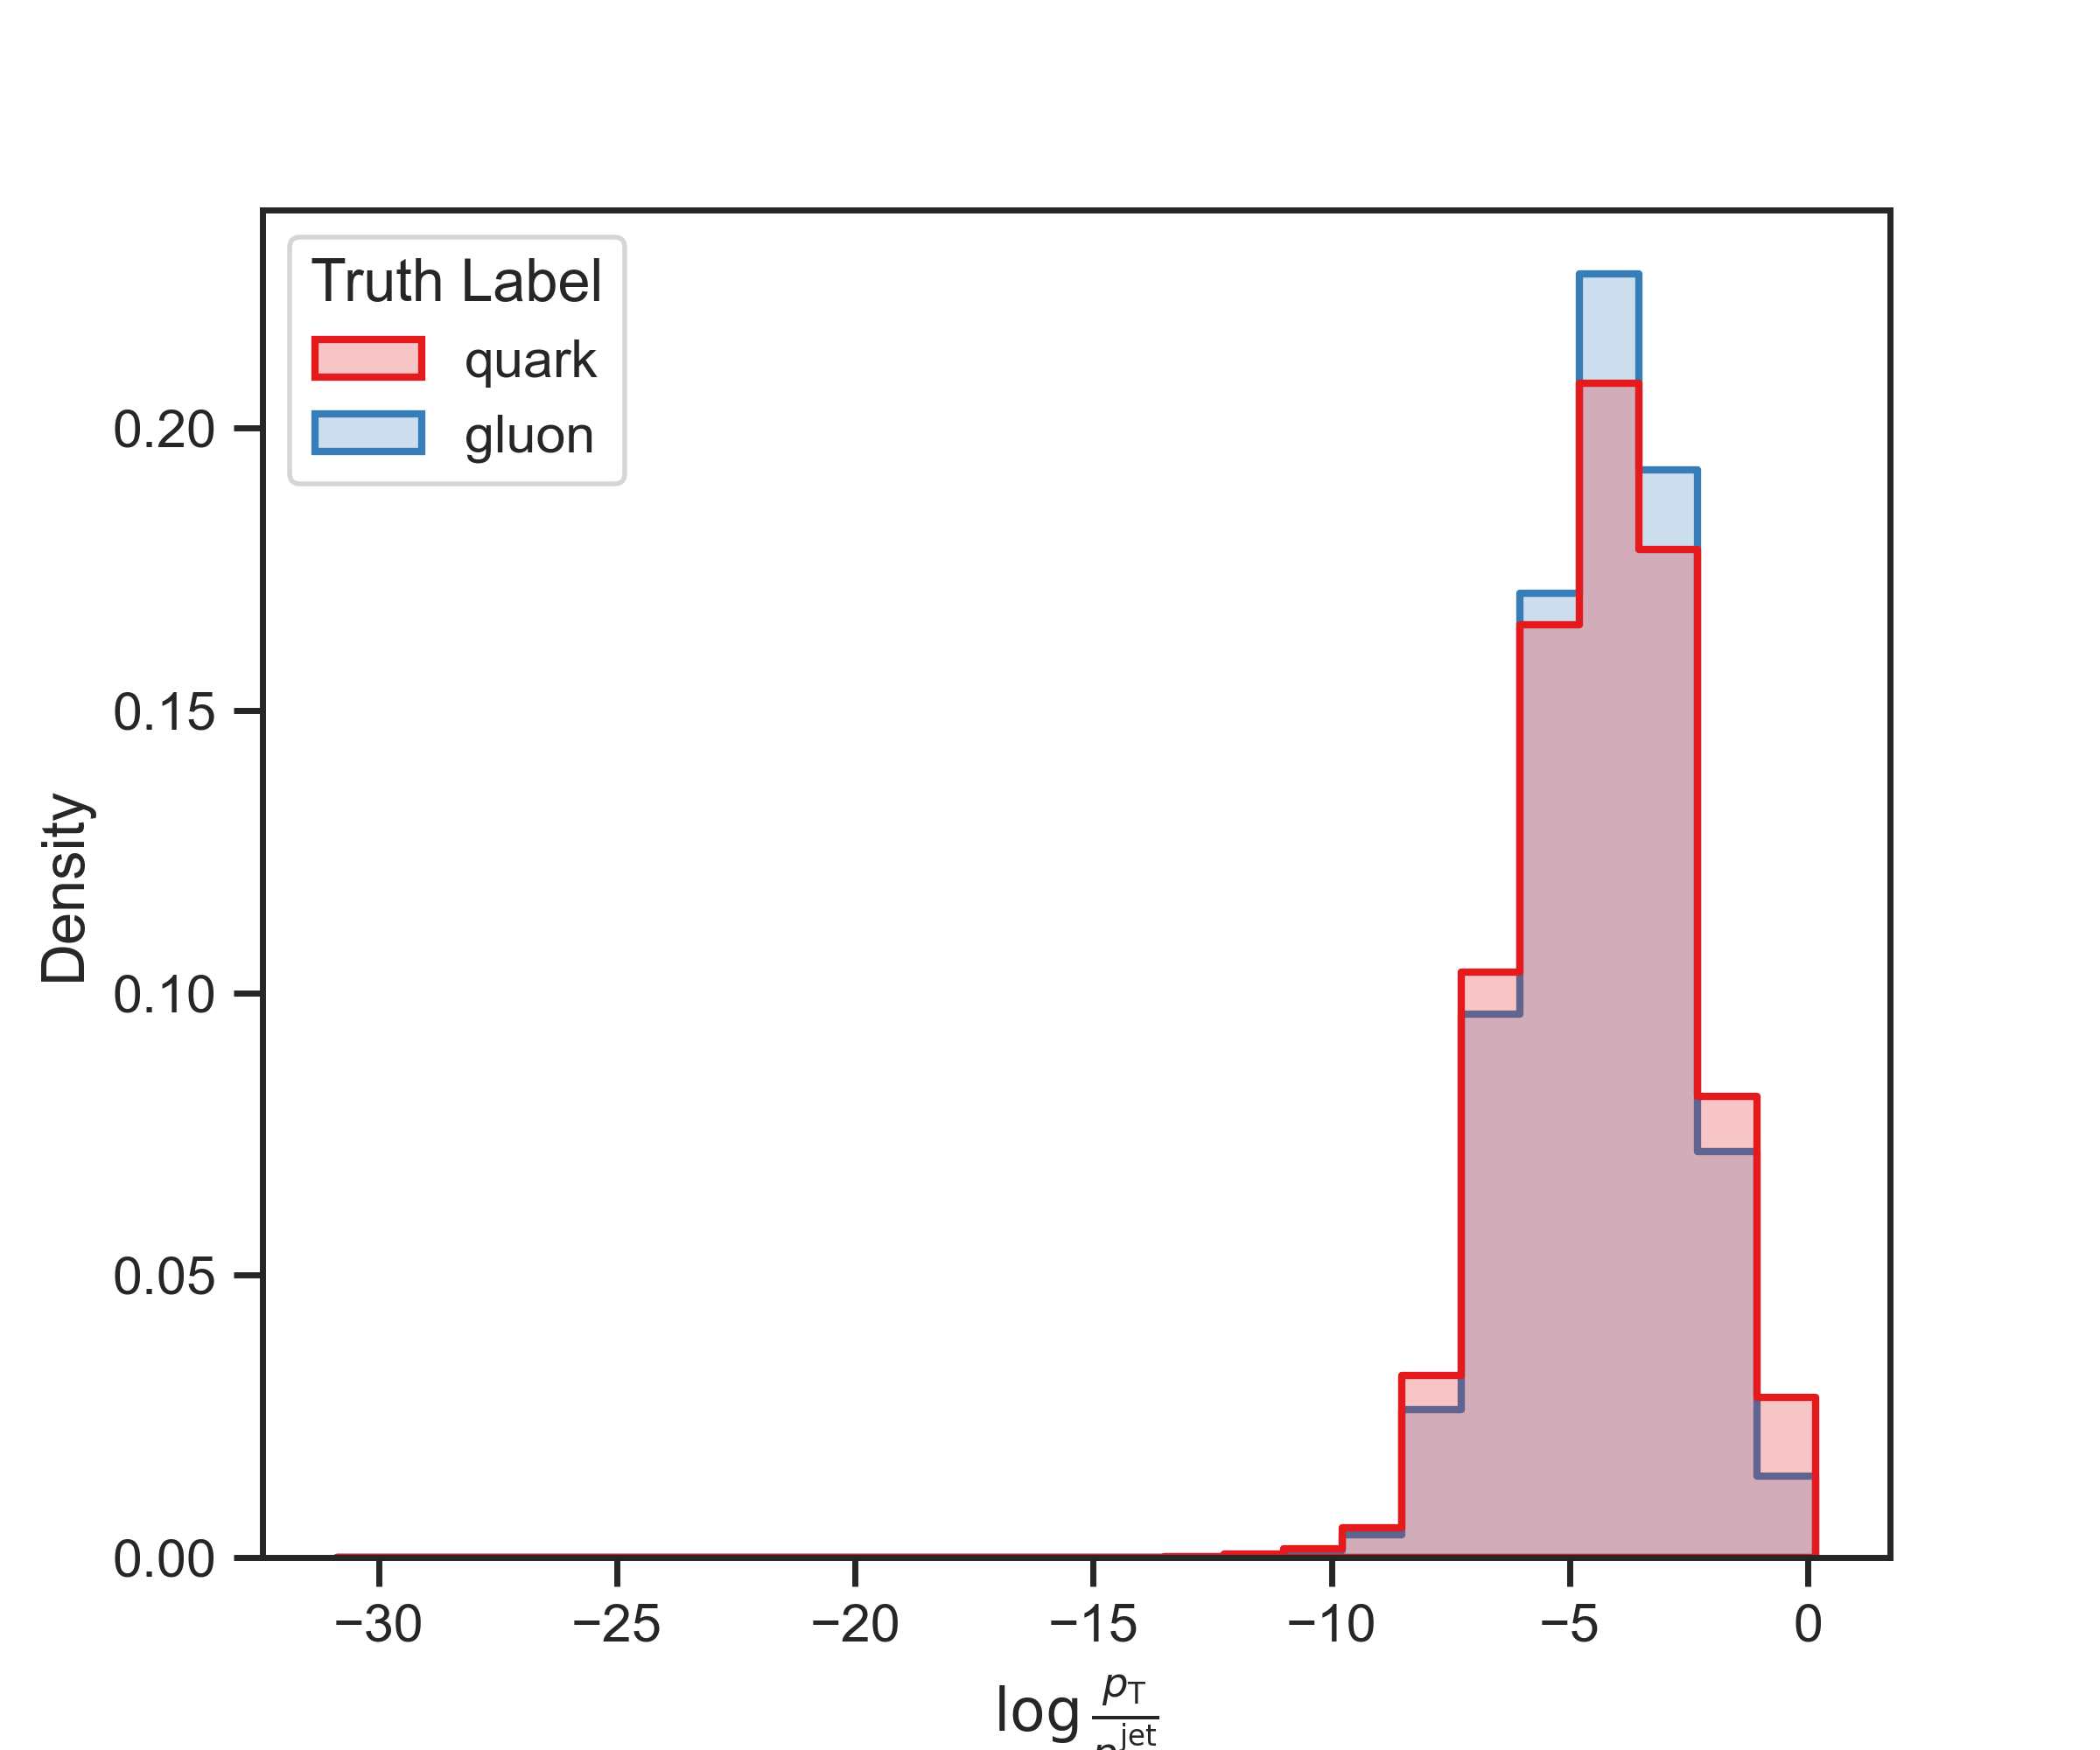
\includegraphics[width=\linewidth]{src/plots/distributions/PFOs/log_PT|PTjet.png}
        \caption{PFO $\log\pT / \pT^{\mathrm{jet}}$}
        \label{fig:app_pfo_log_pT_over_pT_jet}
    \end{subfigure}
    \begin{subfigure}[t]{0.45\textwidth}
        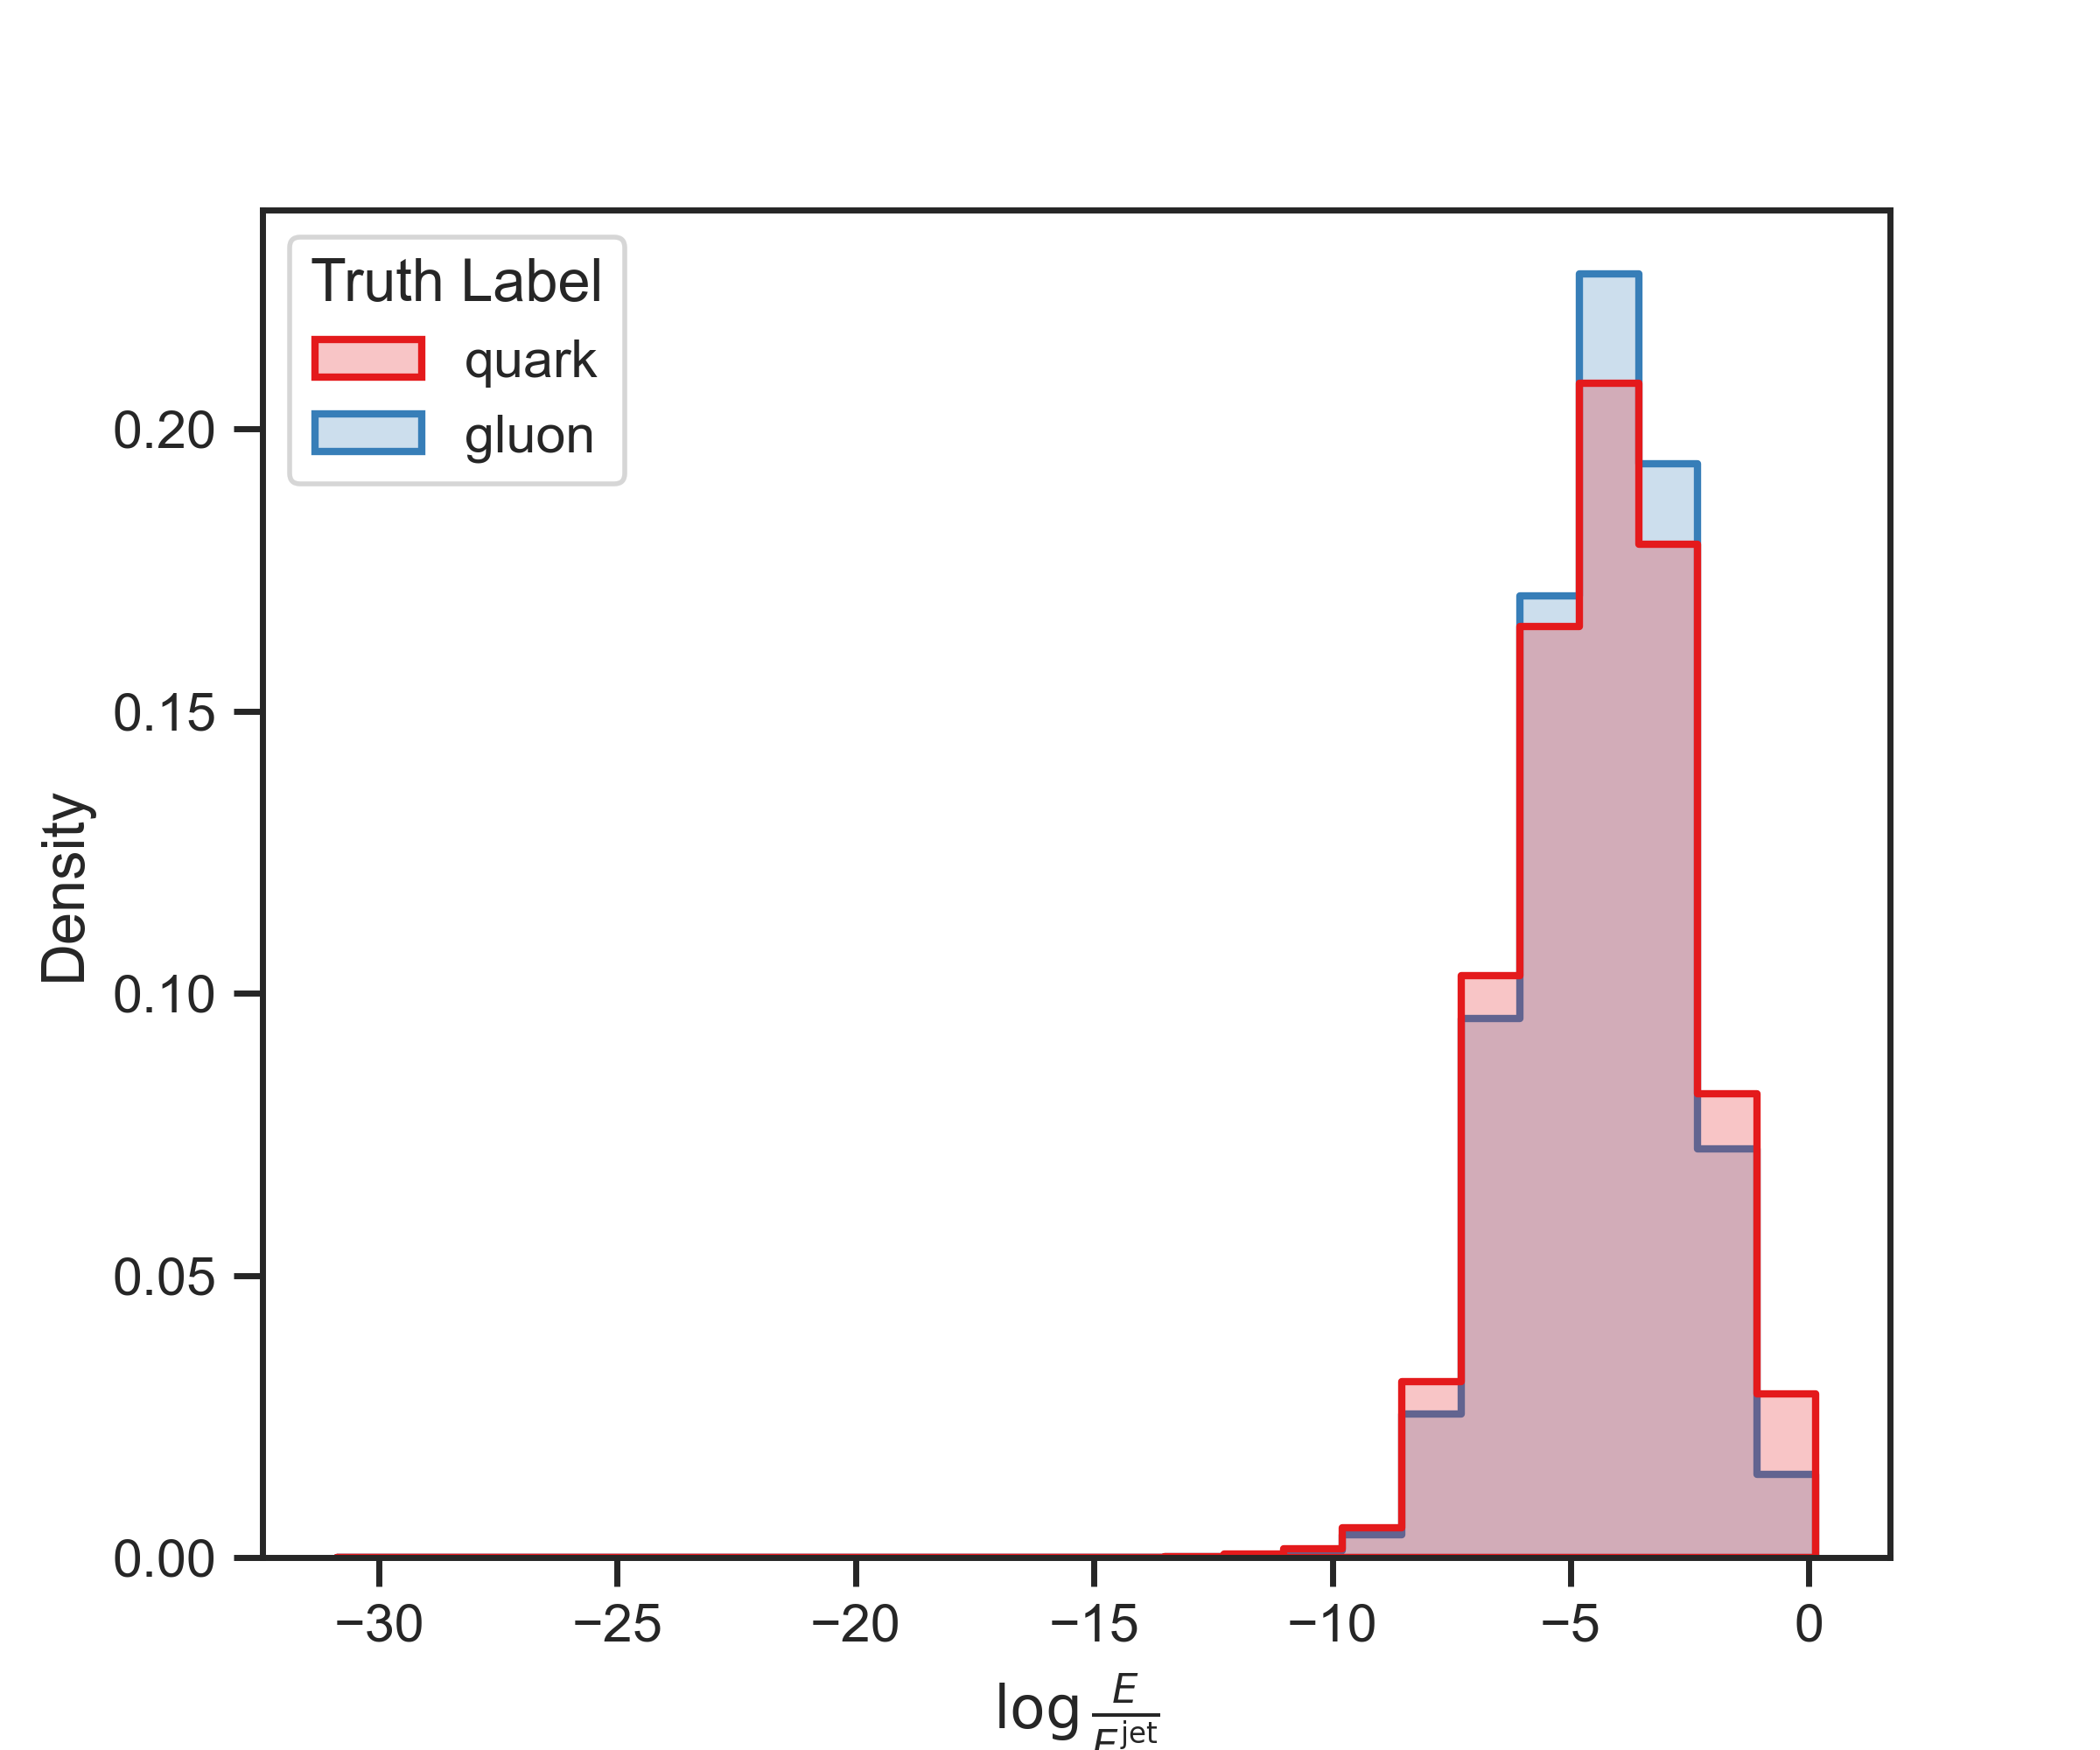
\includegraphics[width=\linewidth]{src/plots/distributions/PFOs/log_E|Ejet.png}
        \caption{PFO $\log E / E^{\mathrm{jet}}$}
        \label{fig:app_pfo_log_E_over_E_jet}
    \end{subfigure}
\caption{Distributions of PFO variables part 1.}
\label{fig:app_pfo_variables_1}
\end{figure}

\begin{figure}[!htb]
    \begin{subfigure}[t]{0.45\textwidth}
        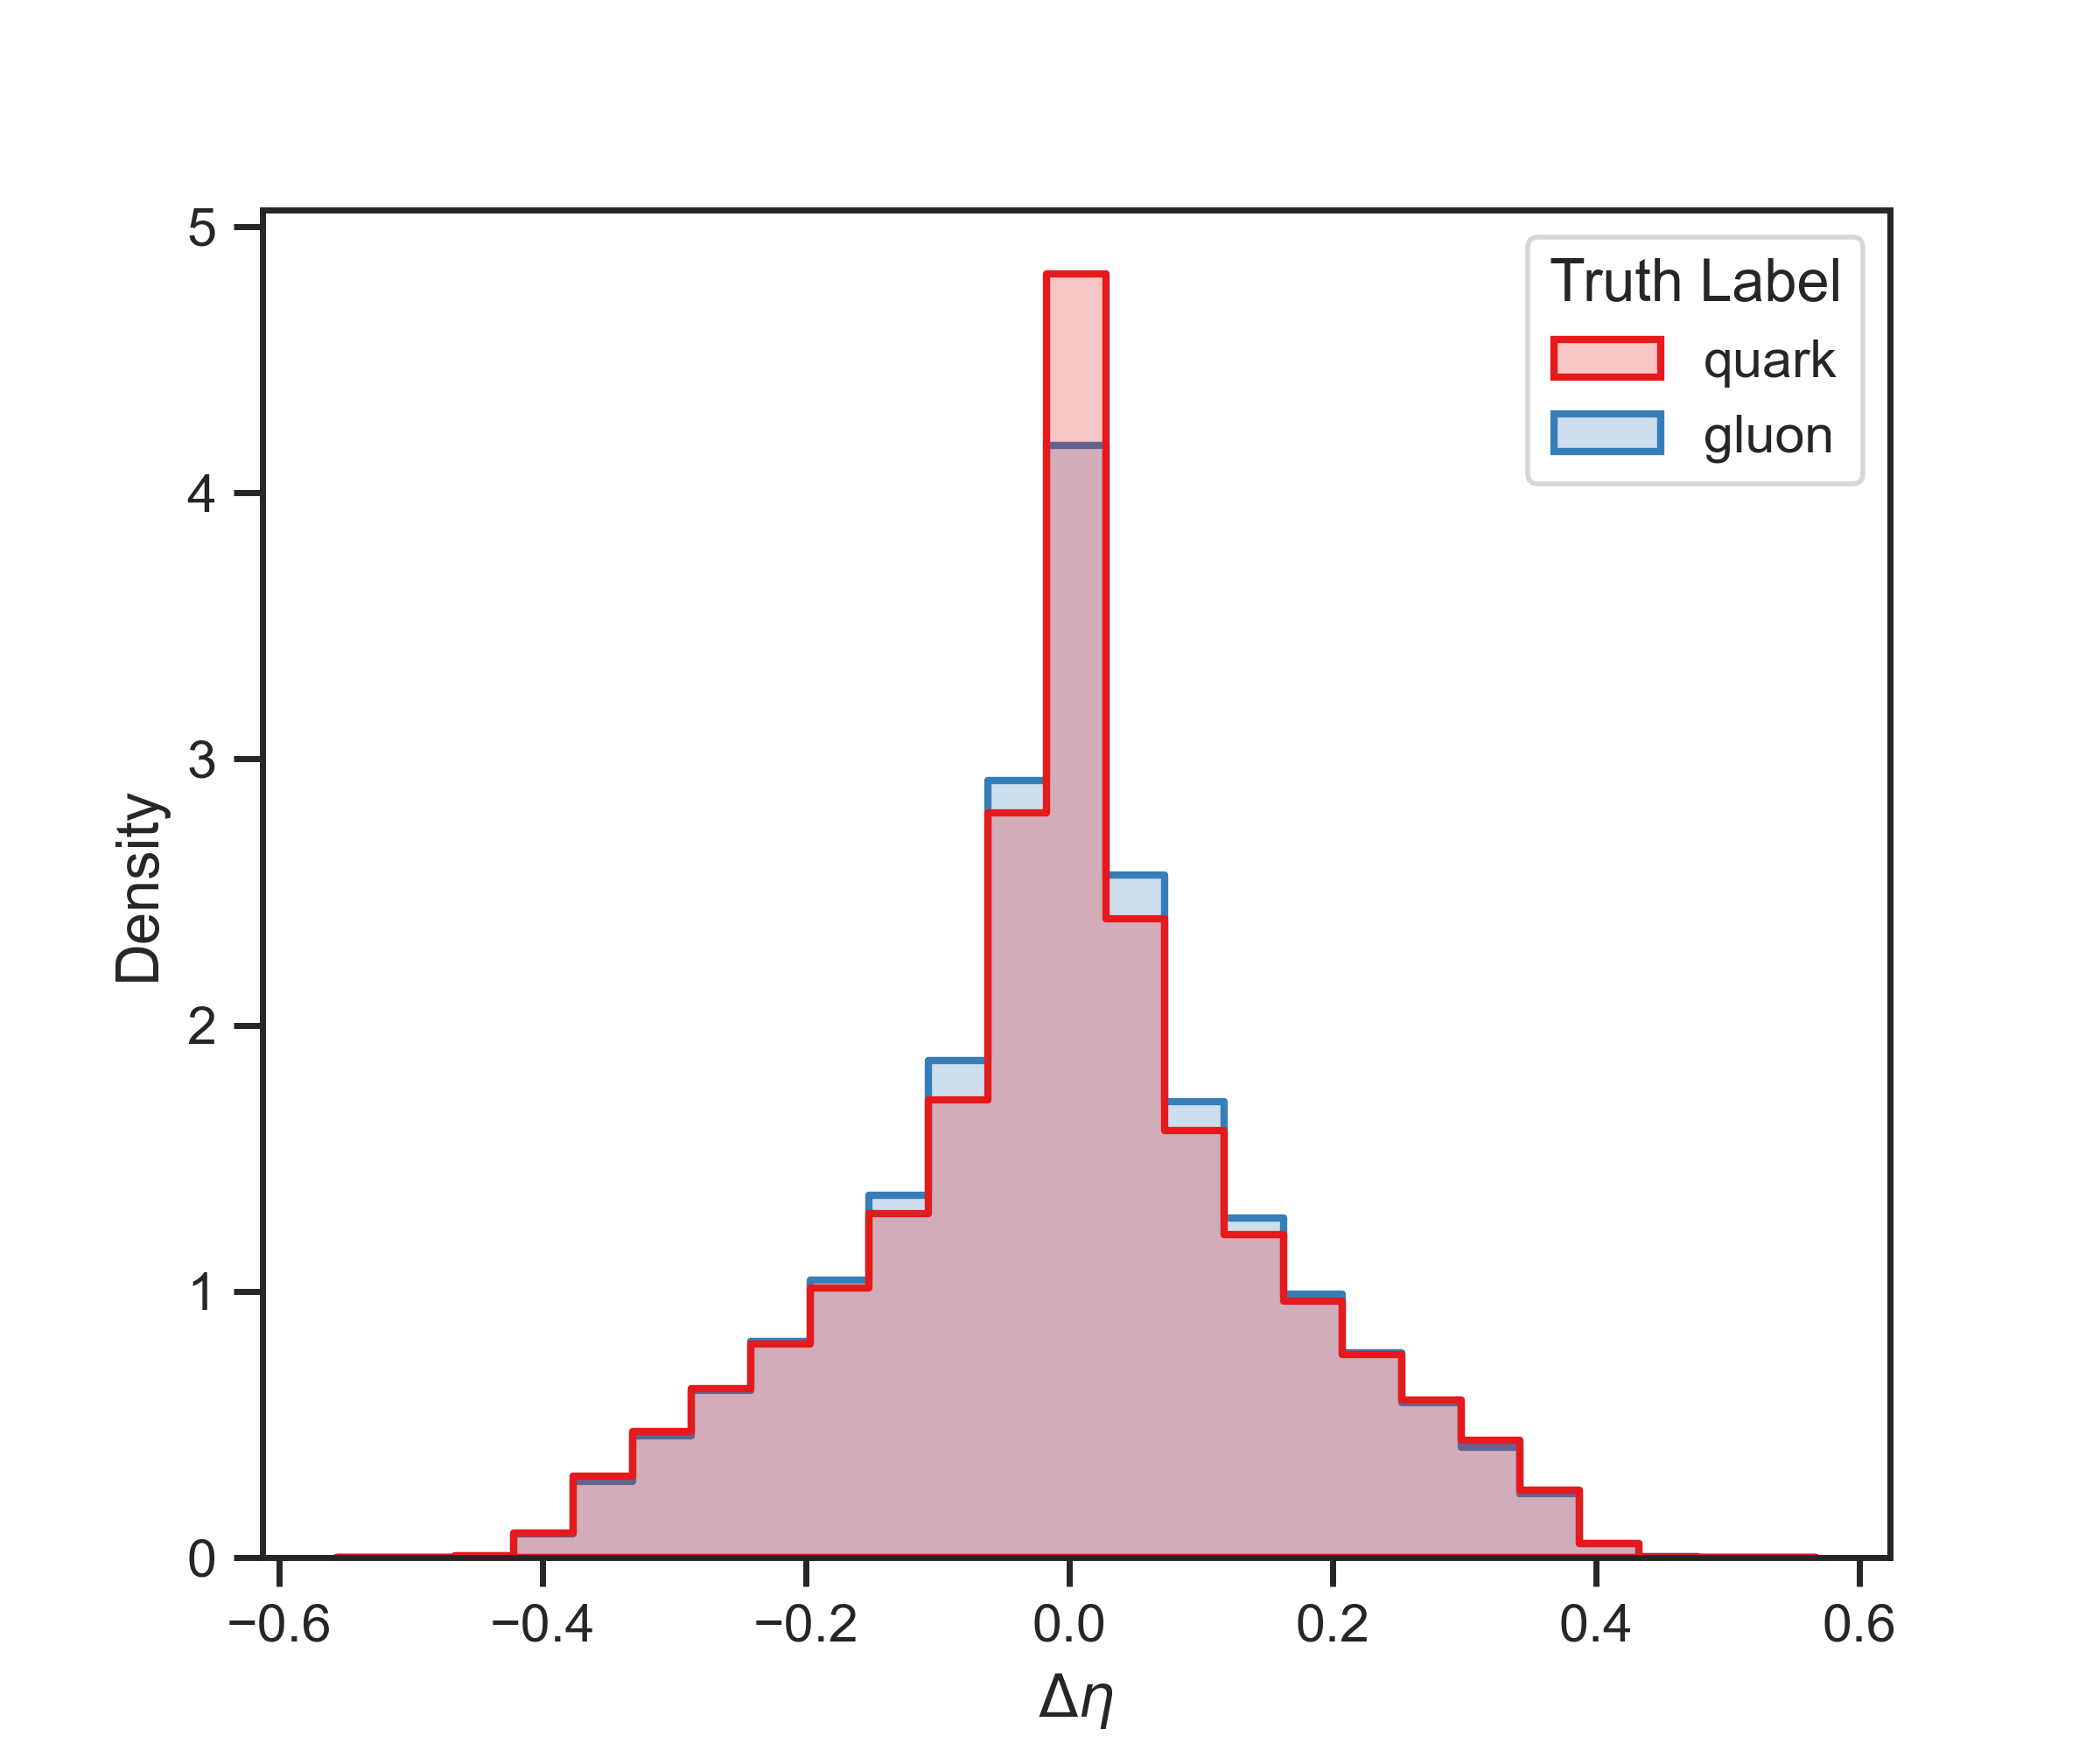
\includegraphics[width=\linewidth]{src/plots/distributions/PFOs/deltaEta.png}
        \caption{PFO $\Delta\eta$}
        \label{fig:app_pfo_deltaEta}
    \end{subfigure}
    \begin{subfigure}[t]{0.45\textwidth}
        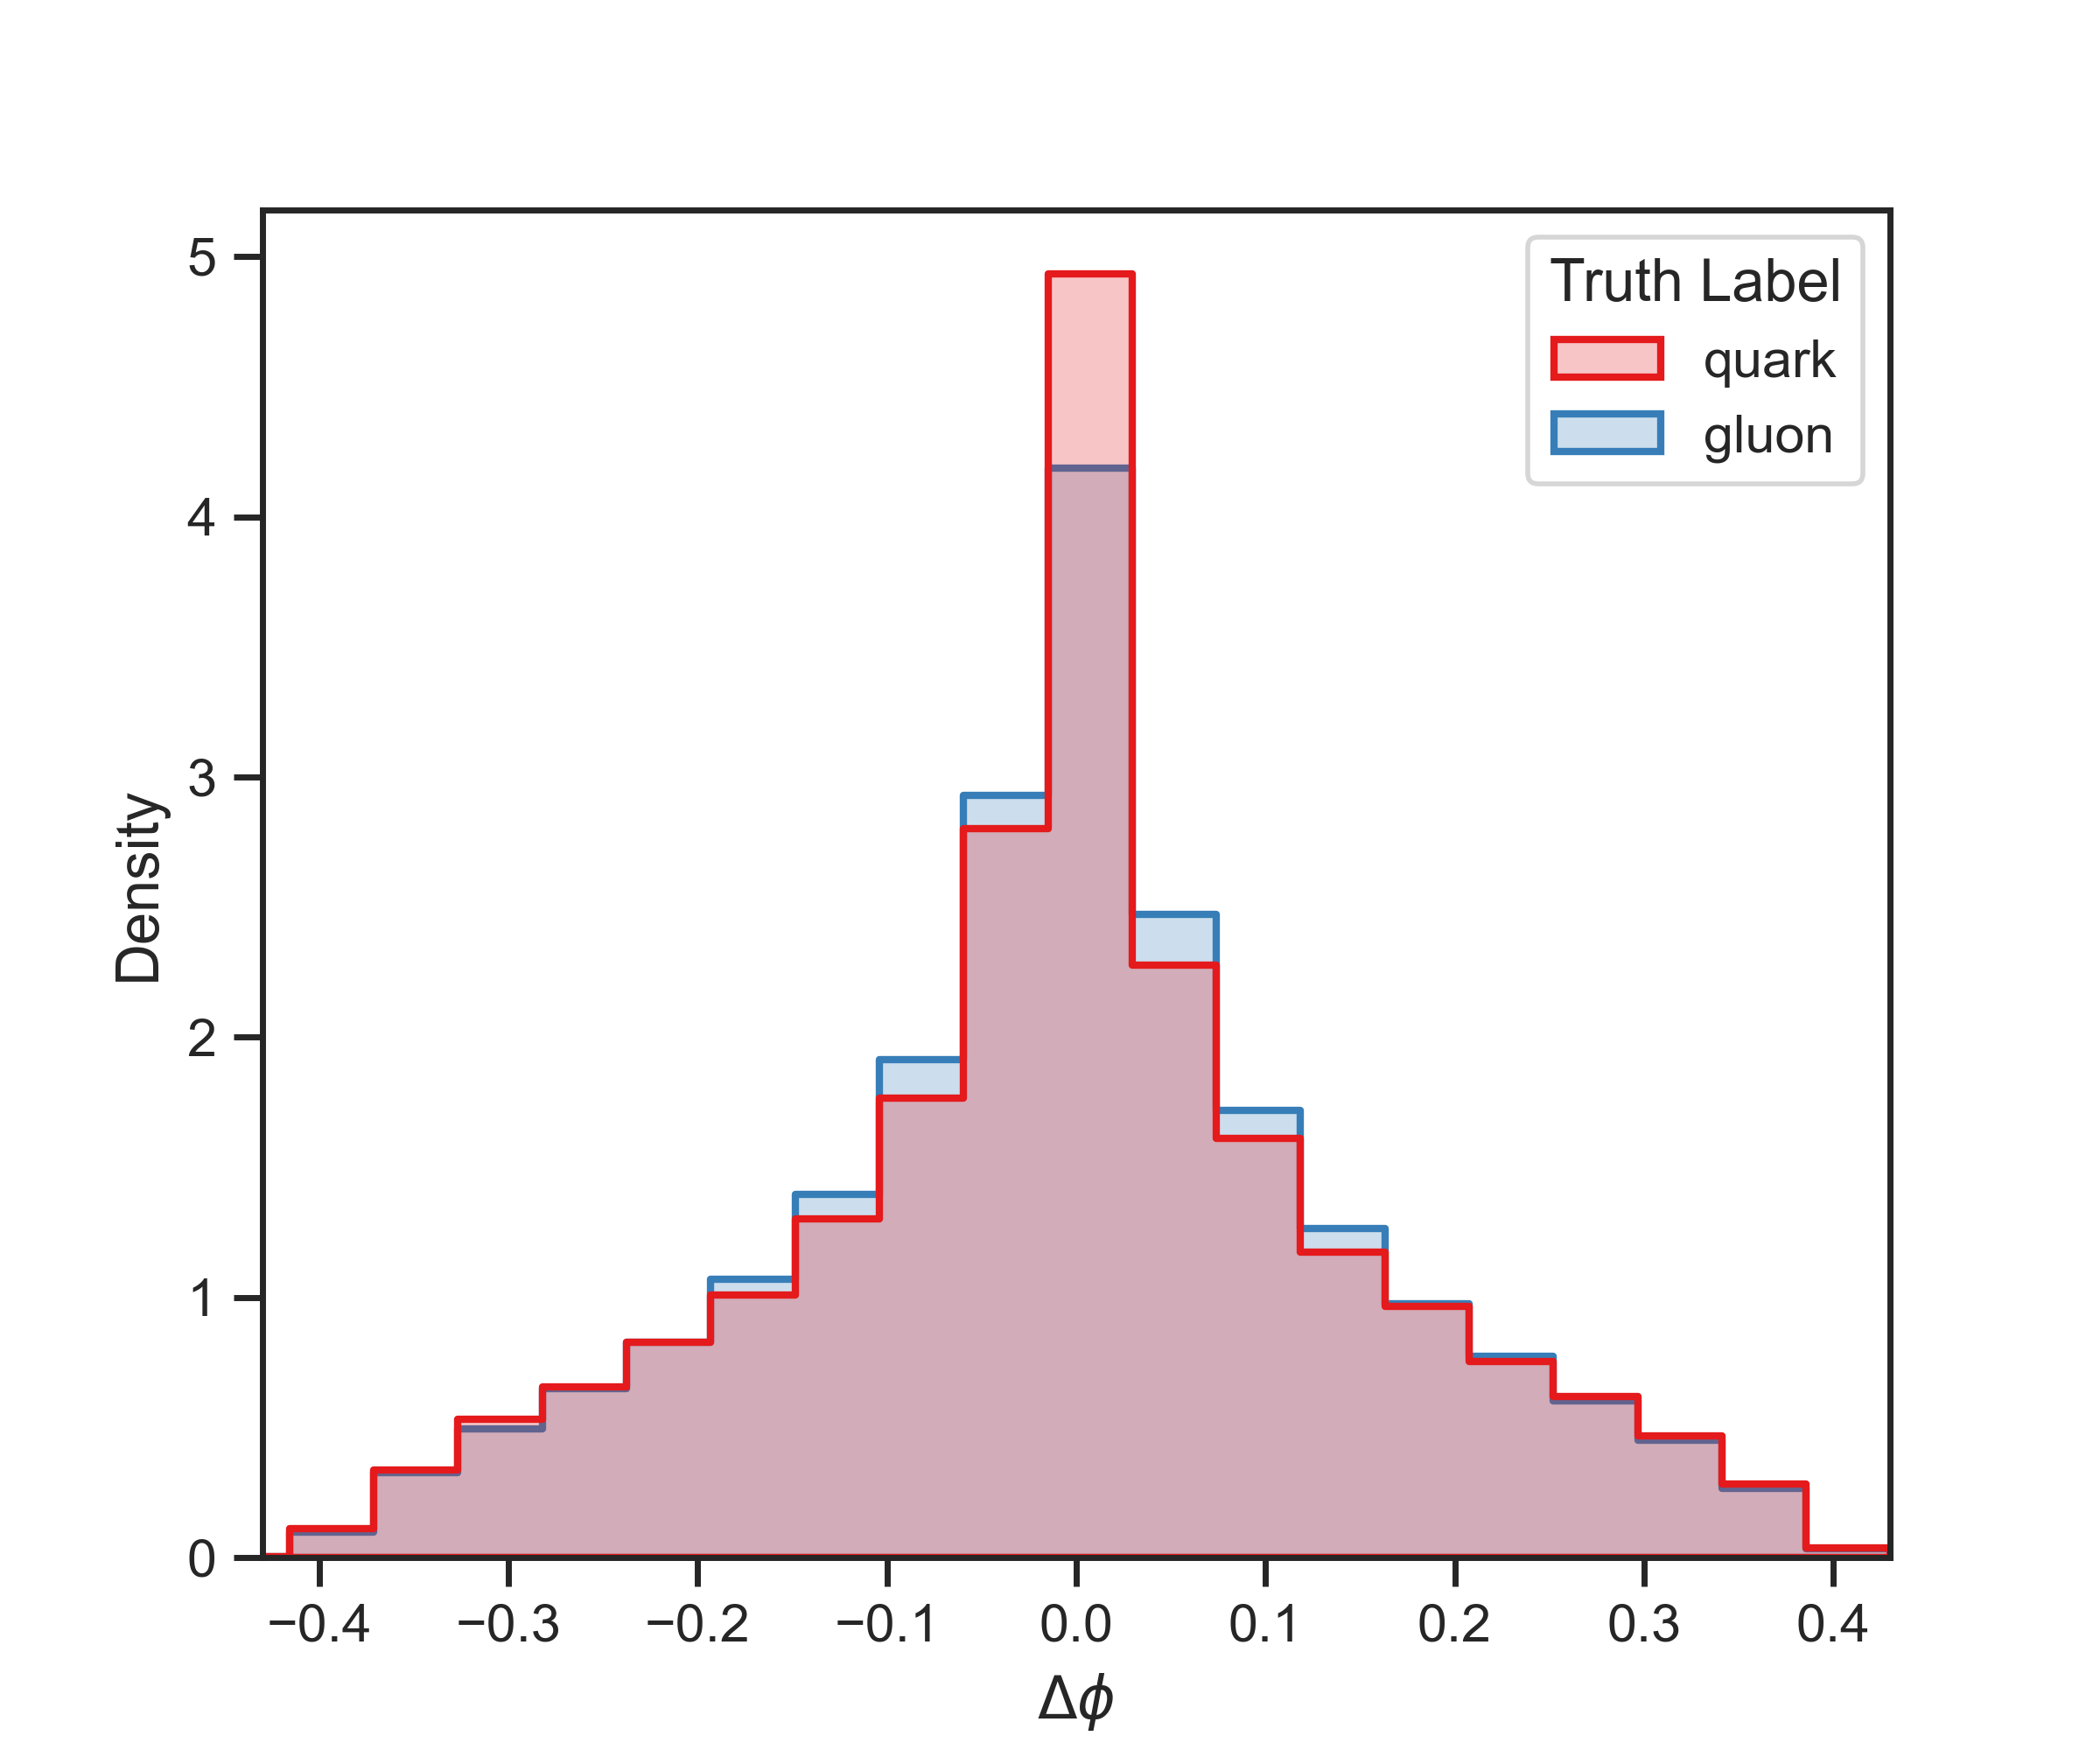
\includegraphics[width=\linewidth]{src/plots/distributions/PFOs/deltaPhi.png}
        \caption{PFO $\Delta\phi$}
        \label{fig:app_pfo_deltaPhi}
    \end{subfigure}
    \begin{subfigure}[t]{0.45\textwidth}
        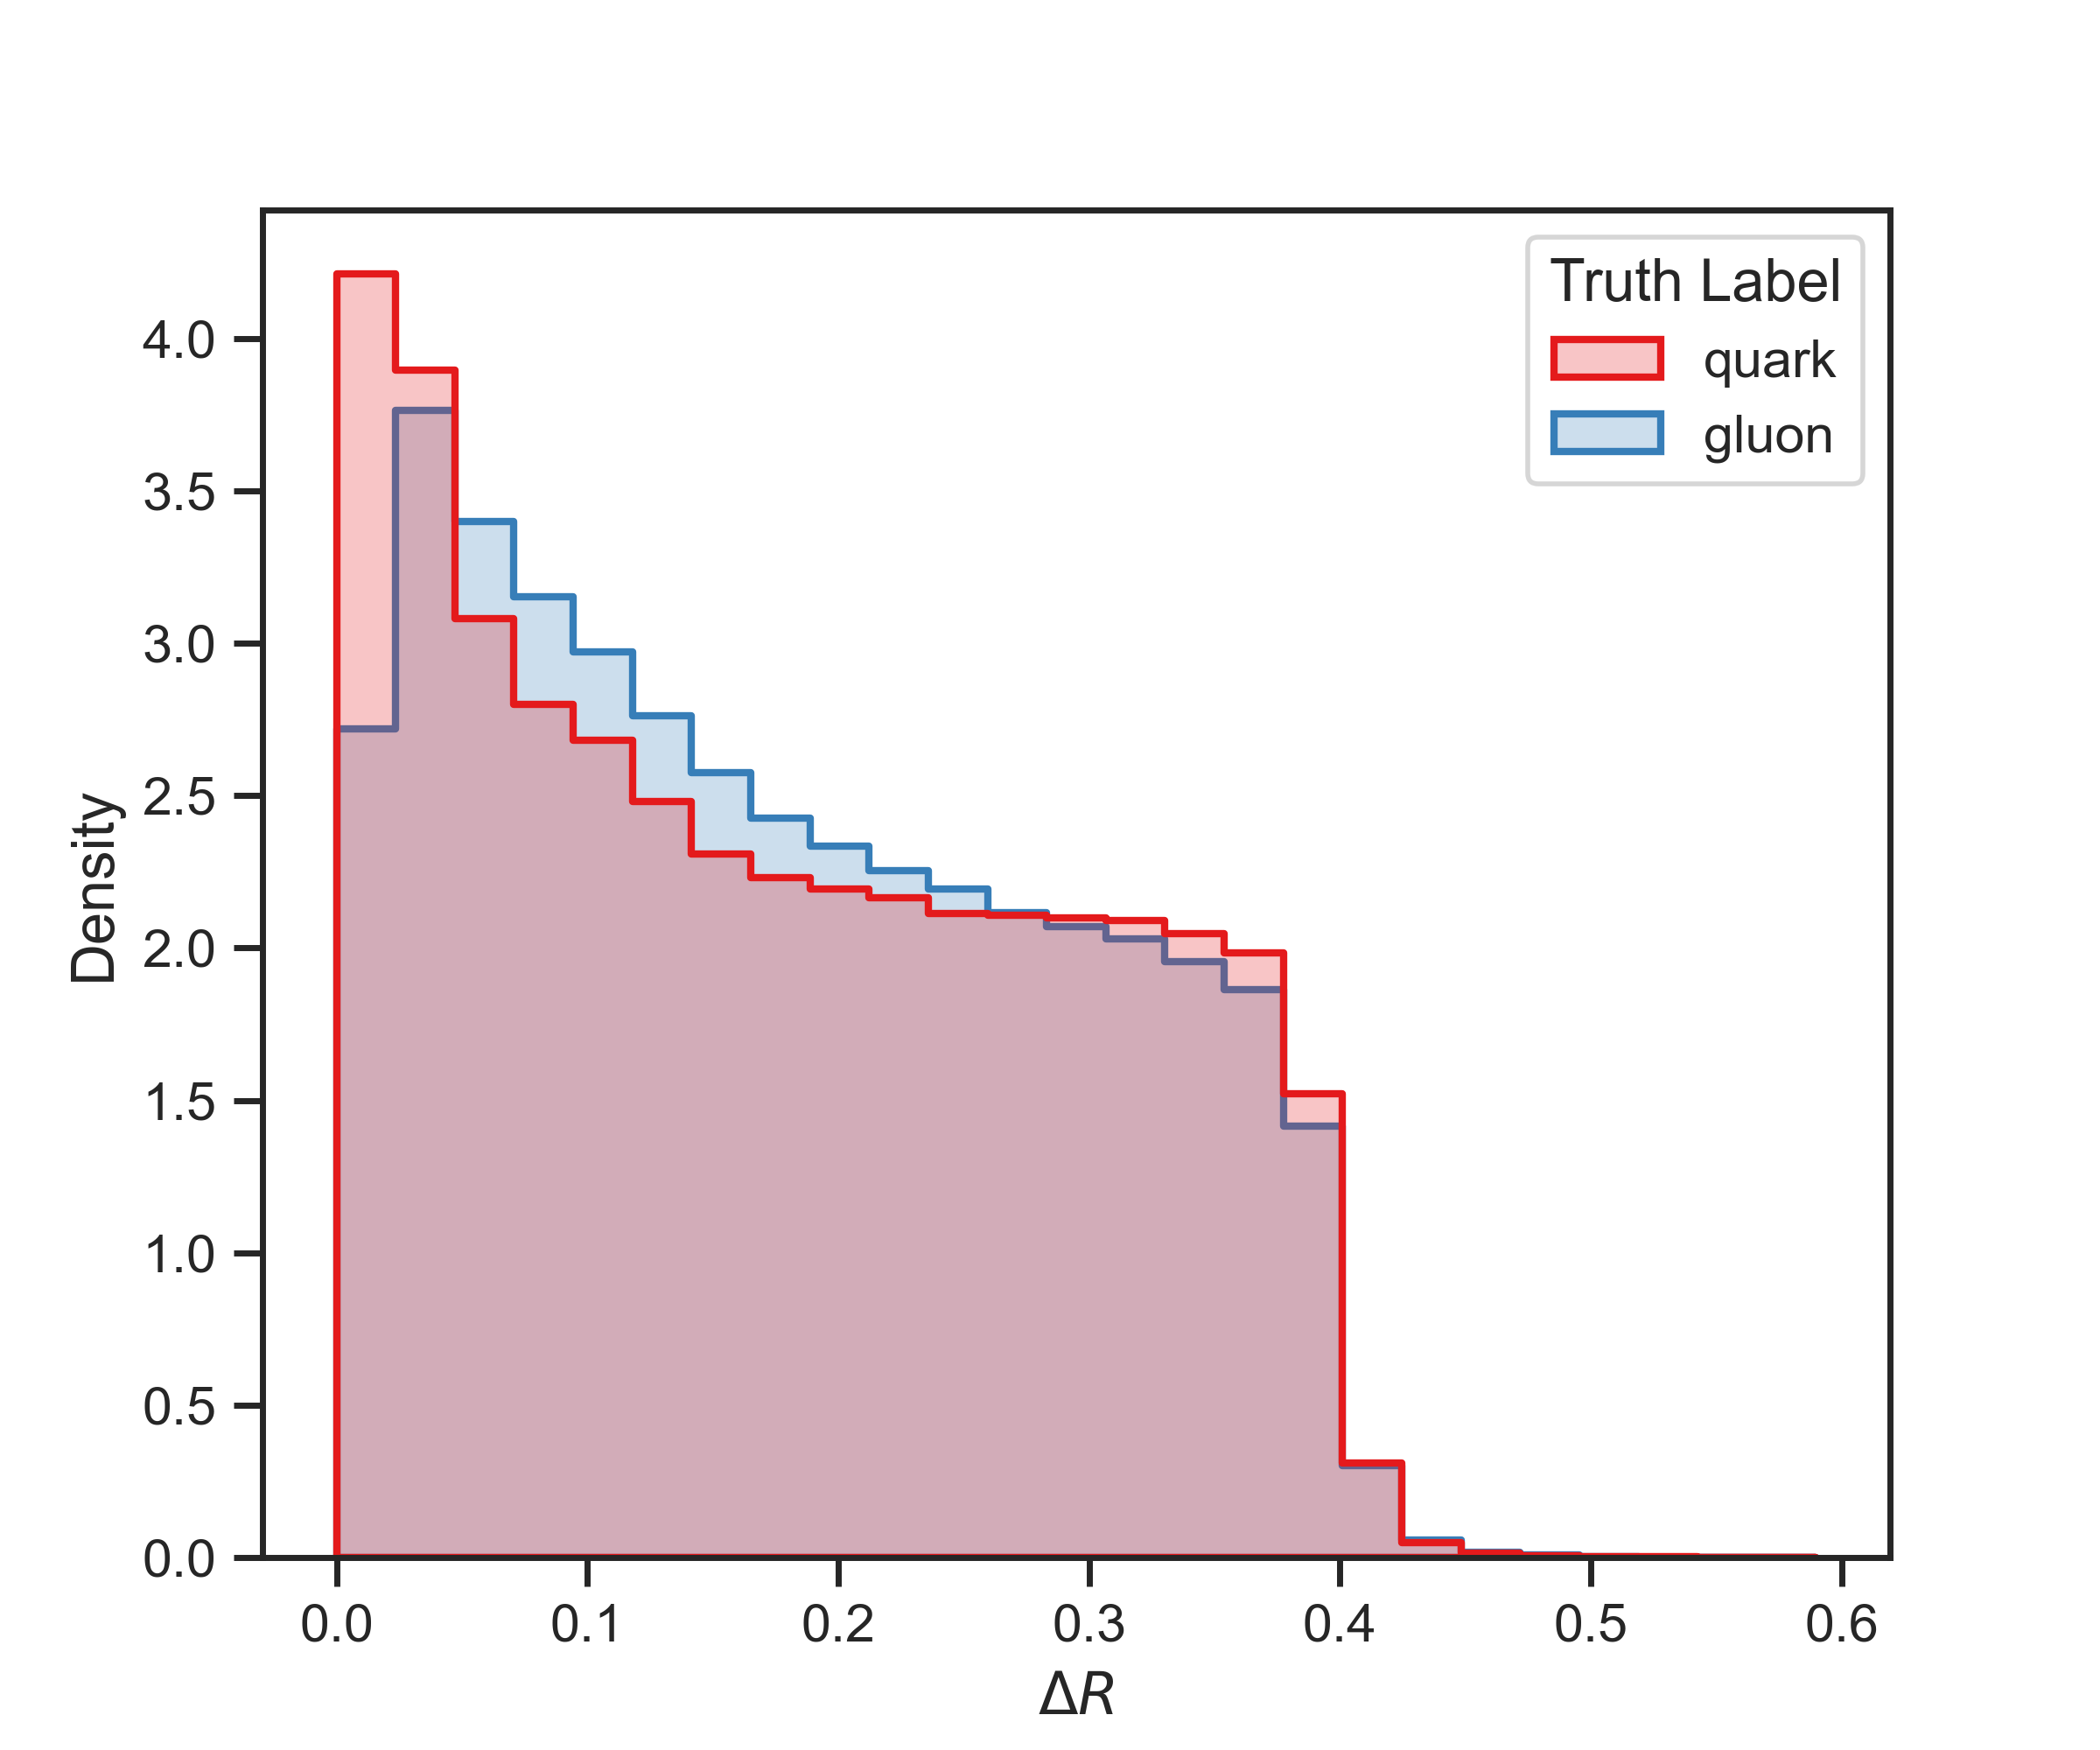
\includegraphics[width=\linewidth]{src/plots/distributions/PFOs/deltaR.png}
        \caption{PFO $\Delta R$}
        \label{fig:app_pfo_deltaR}
    \end{subfigure}
    \begin{subfigure}[t]{0.45\textwidth}
        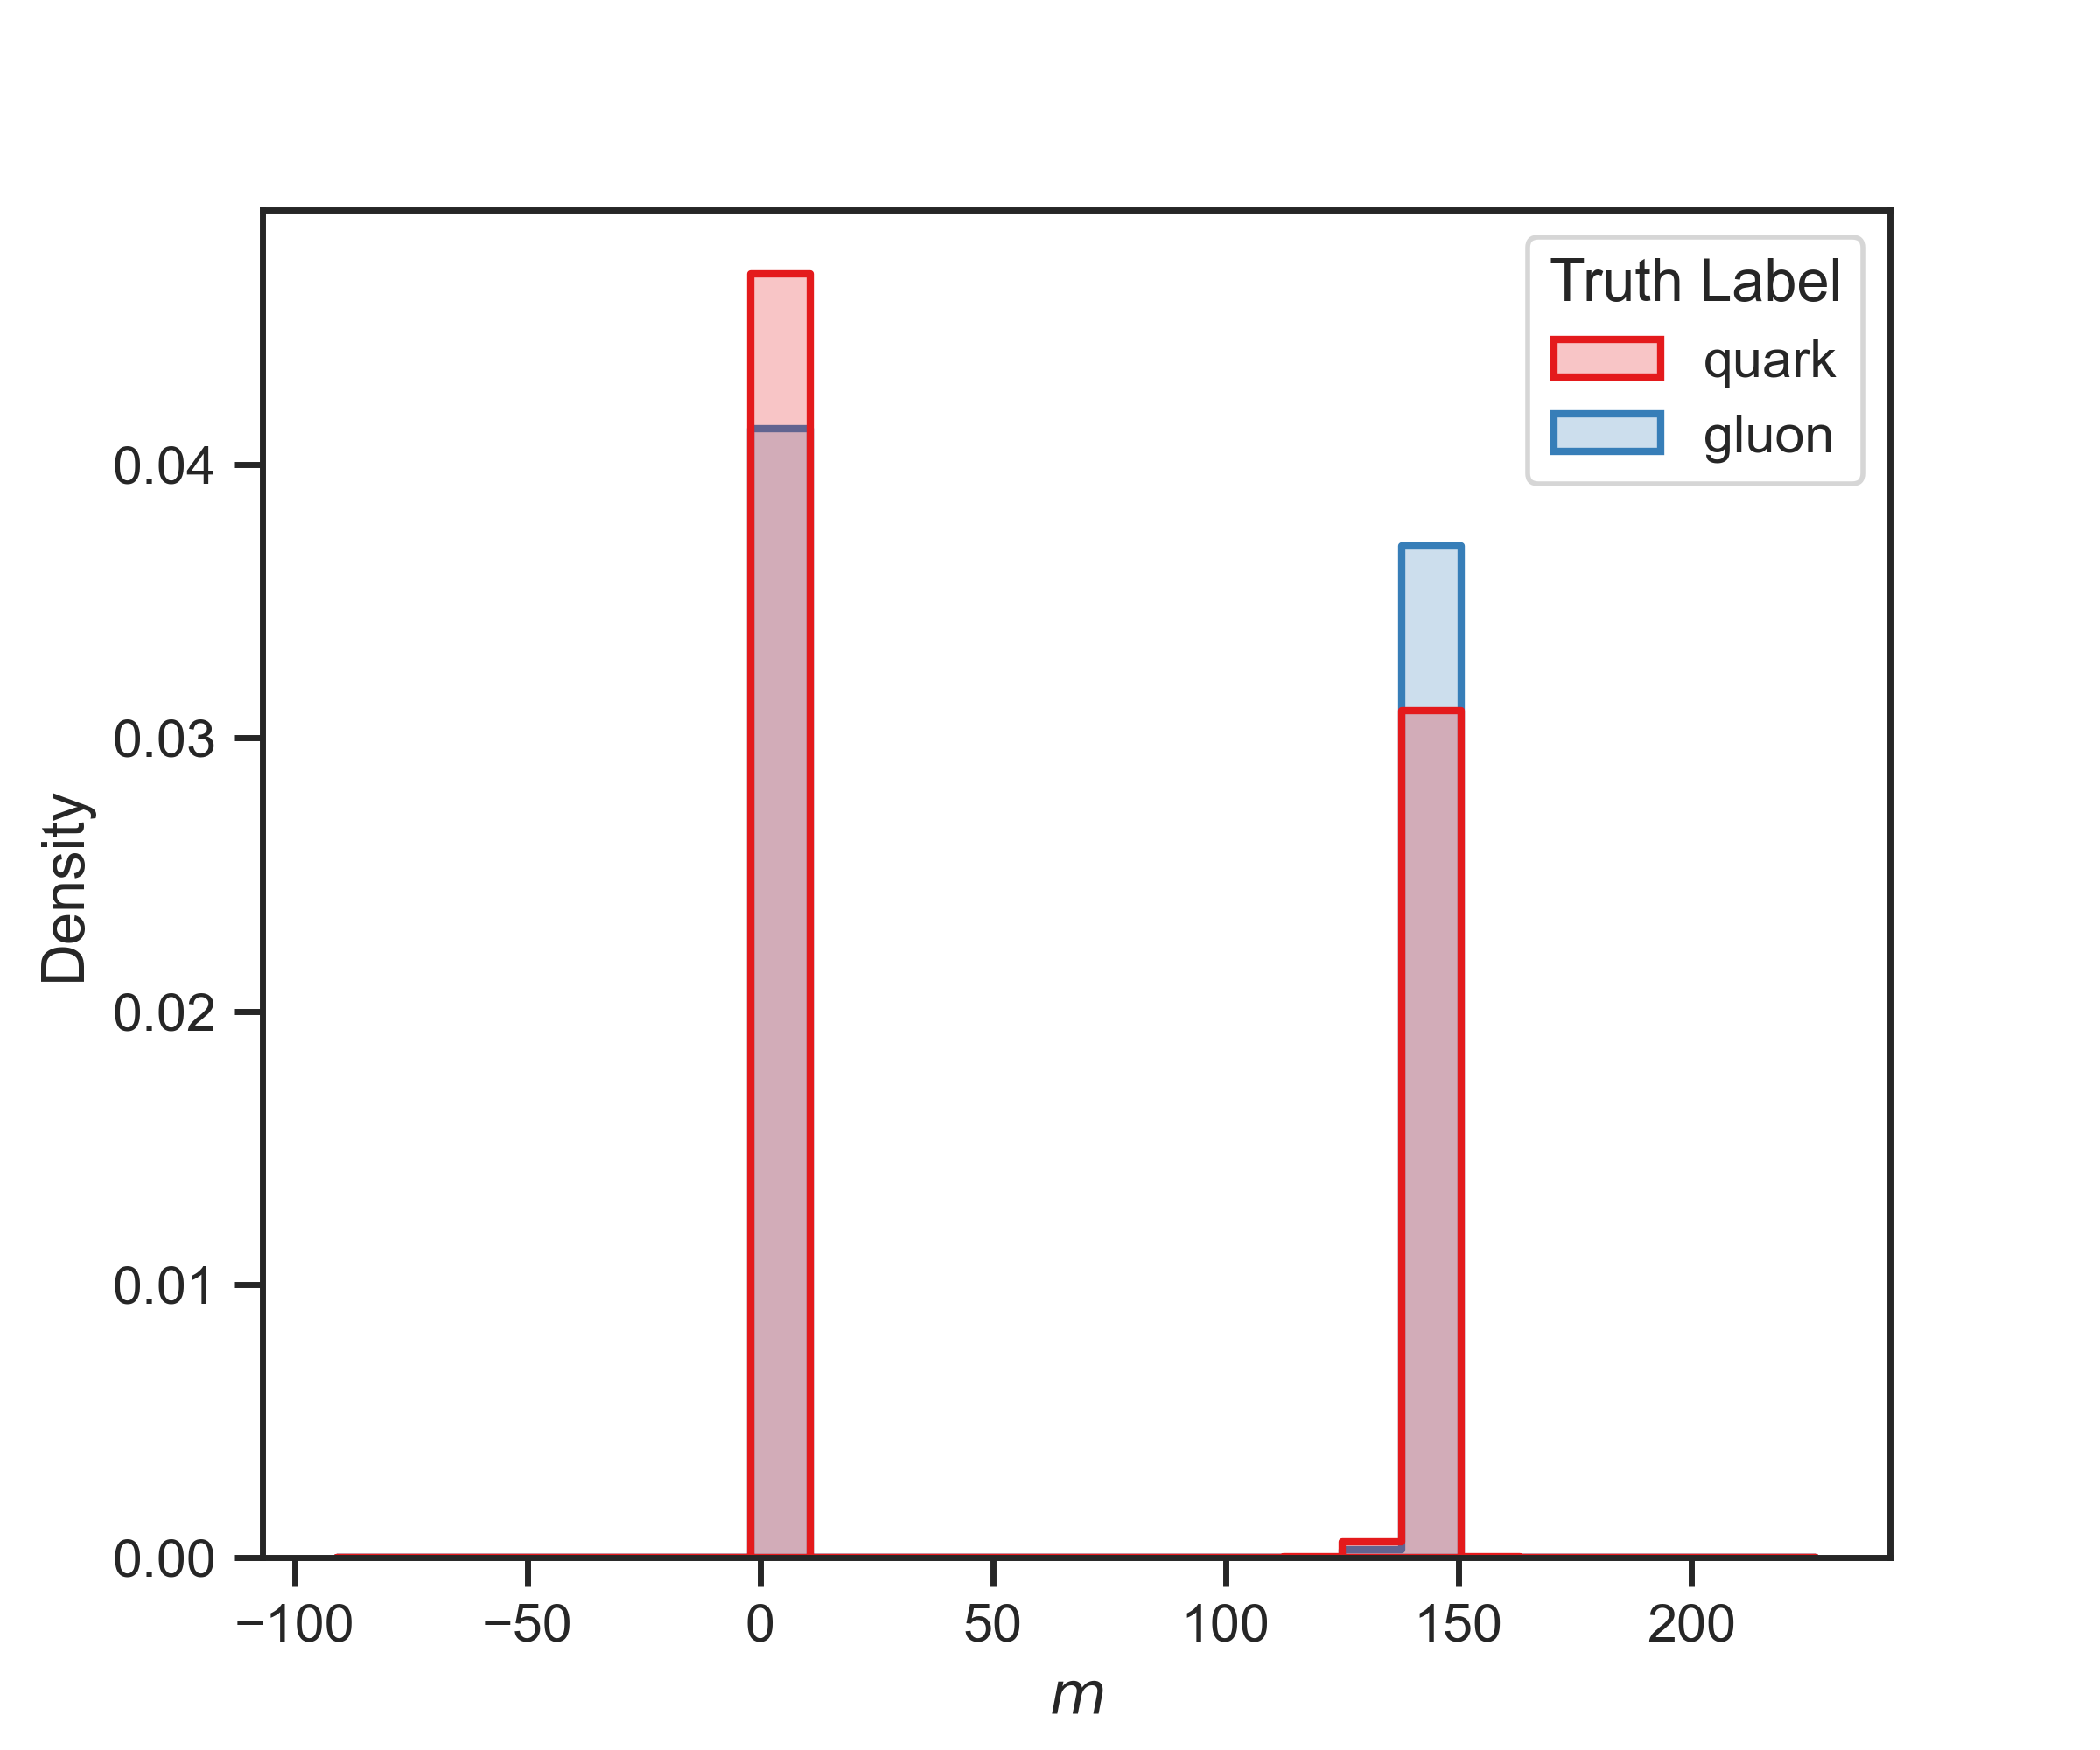
\includegraphics[width=\linewidth]{src/plots/distributions/PFOs/m.png}
        \caption{PFO $m$}
        \label{fig:app_pfo_m}
    \end{subfigure}
    \begin{subfigure}[t]{0.45\textwidth}
        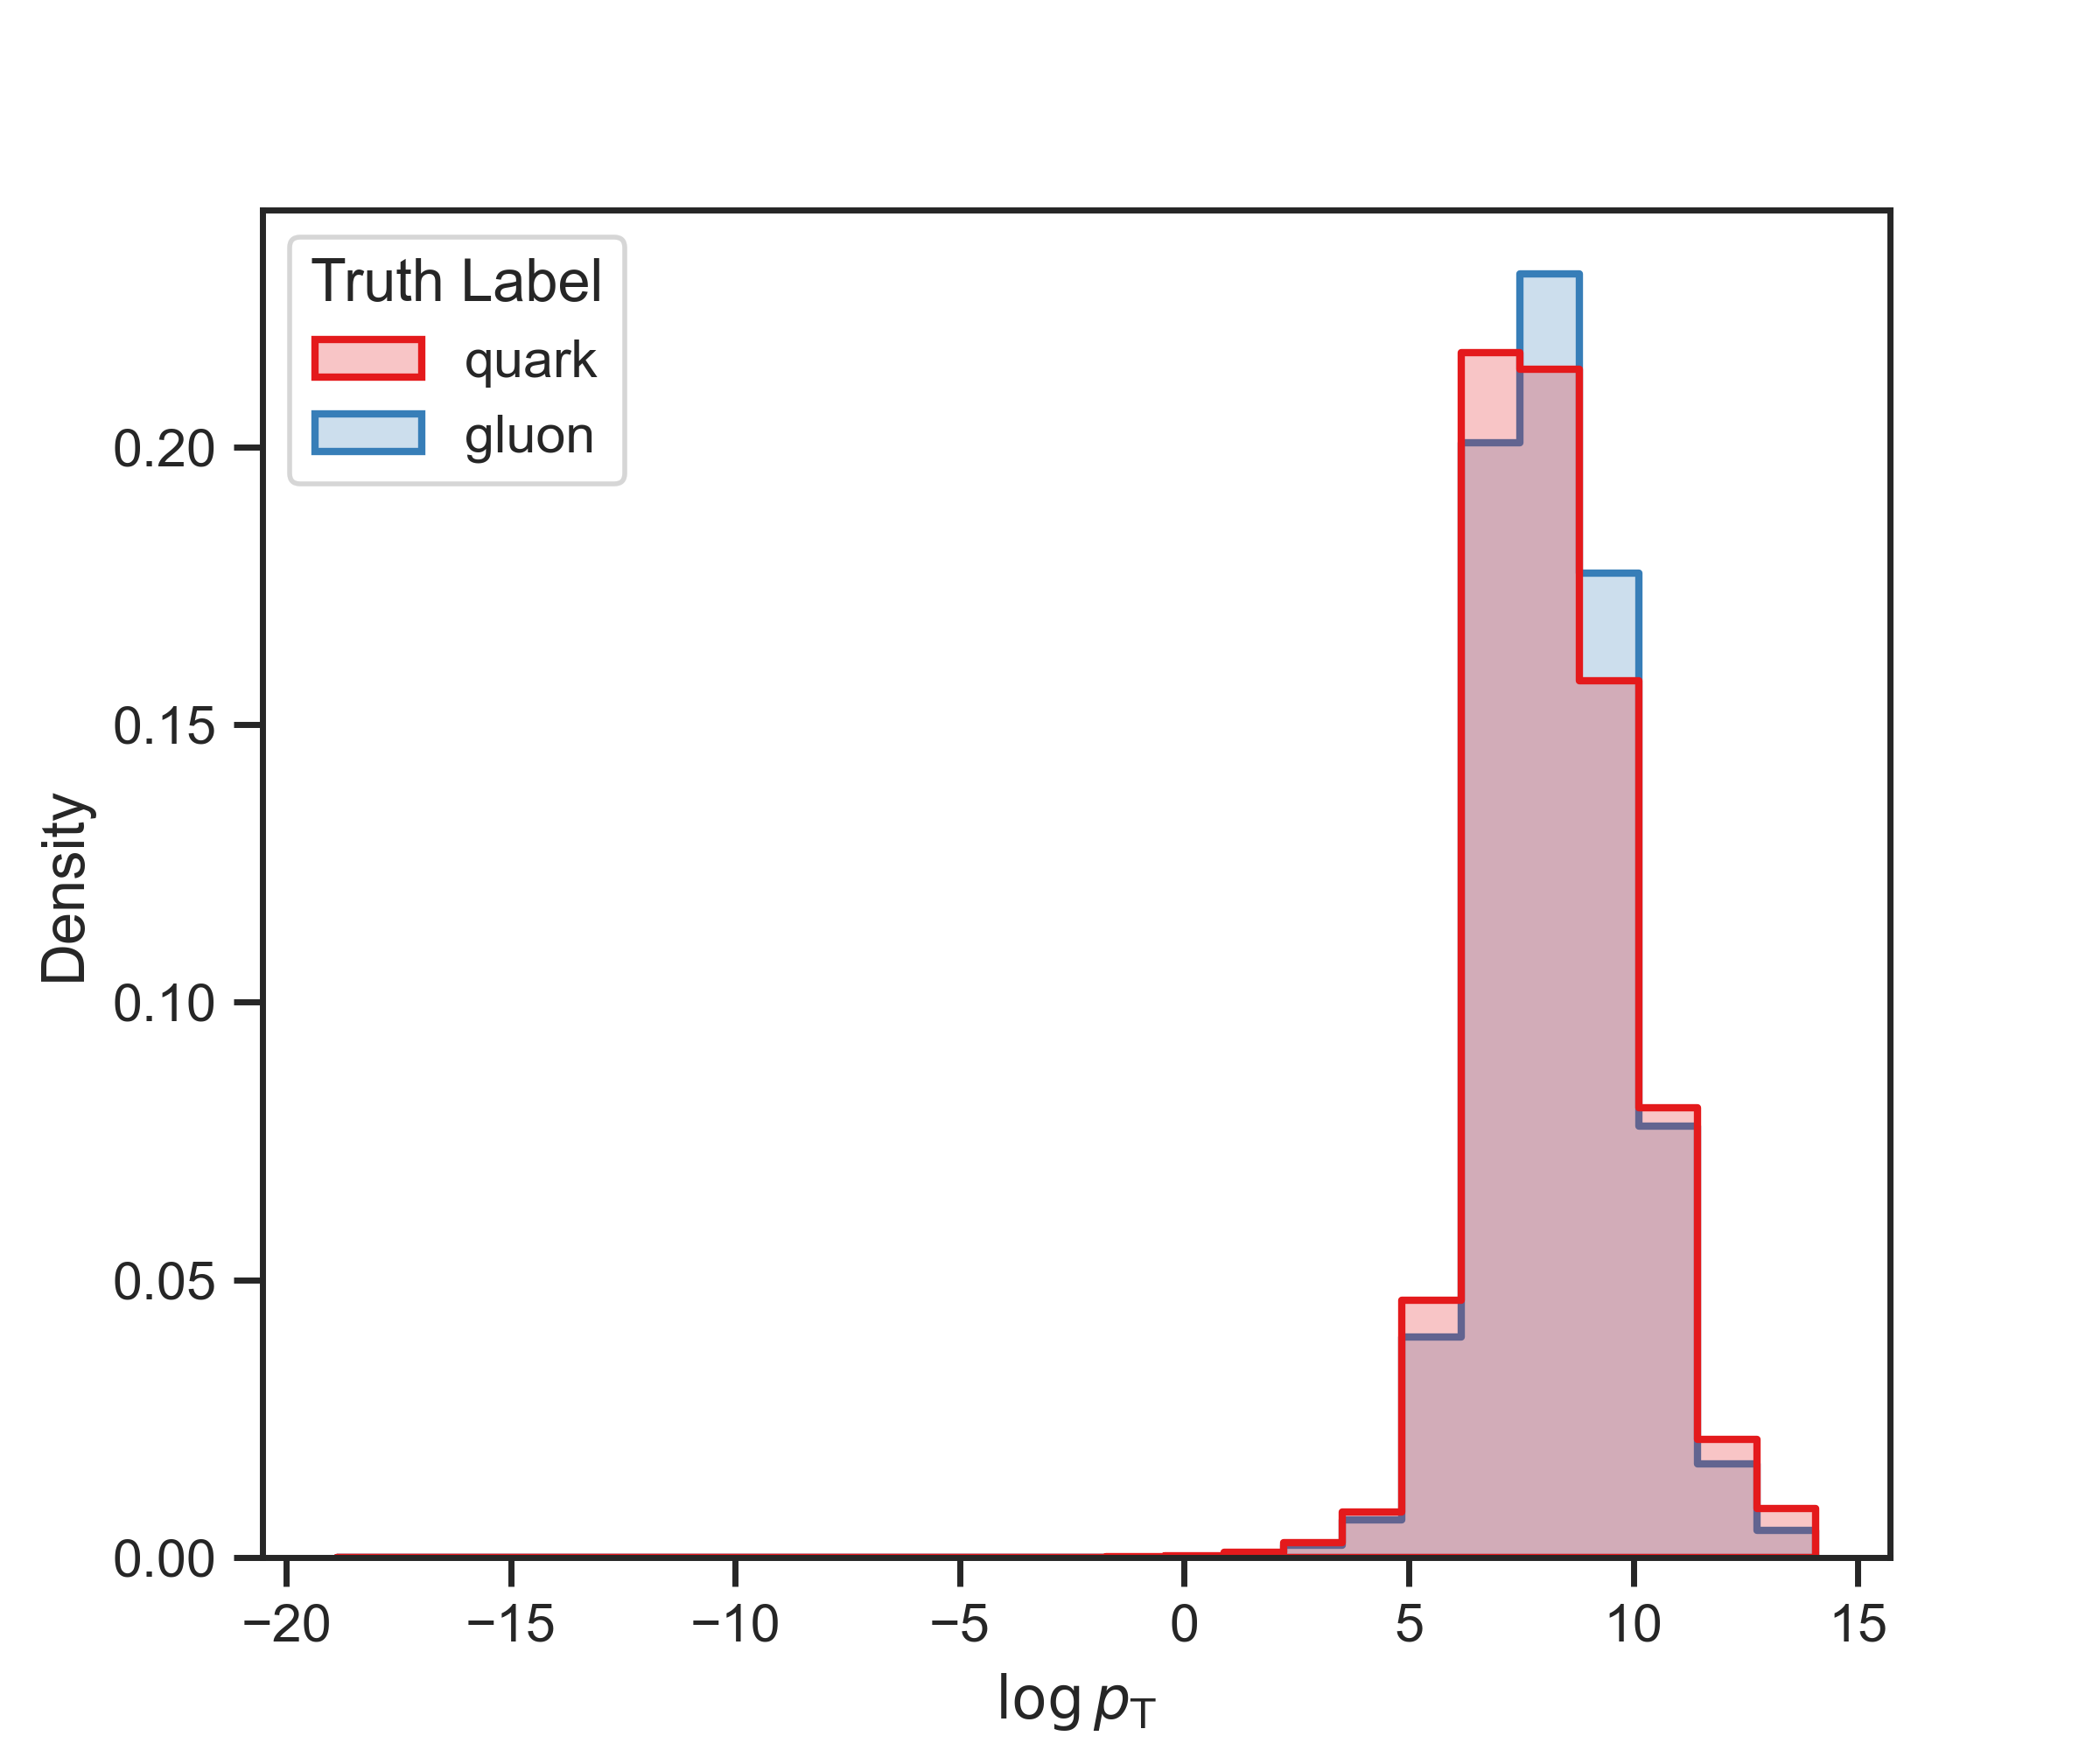
\includegraphics[width=\linewidth]{src/plots/distributions/PFOs/log_pT.png}
        \caption{PFO $\log\pT$}
        \label{fig:app_pfo_log_pT}
    \end{subfigure}
    \begin{subfigure}[t]{0.45\textwidth}
        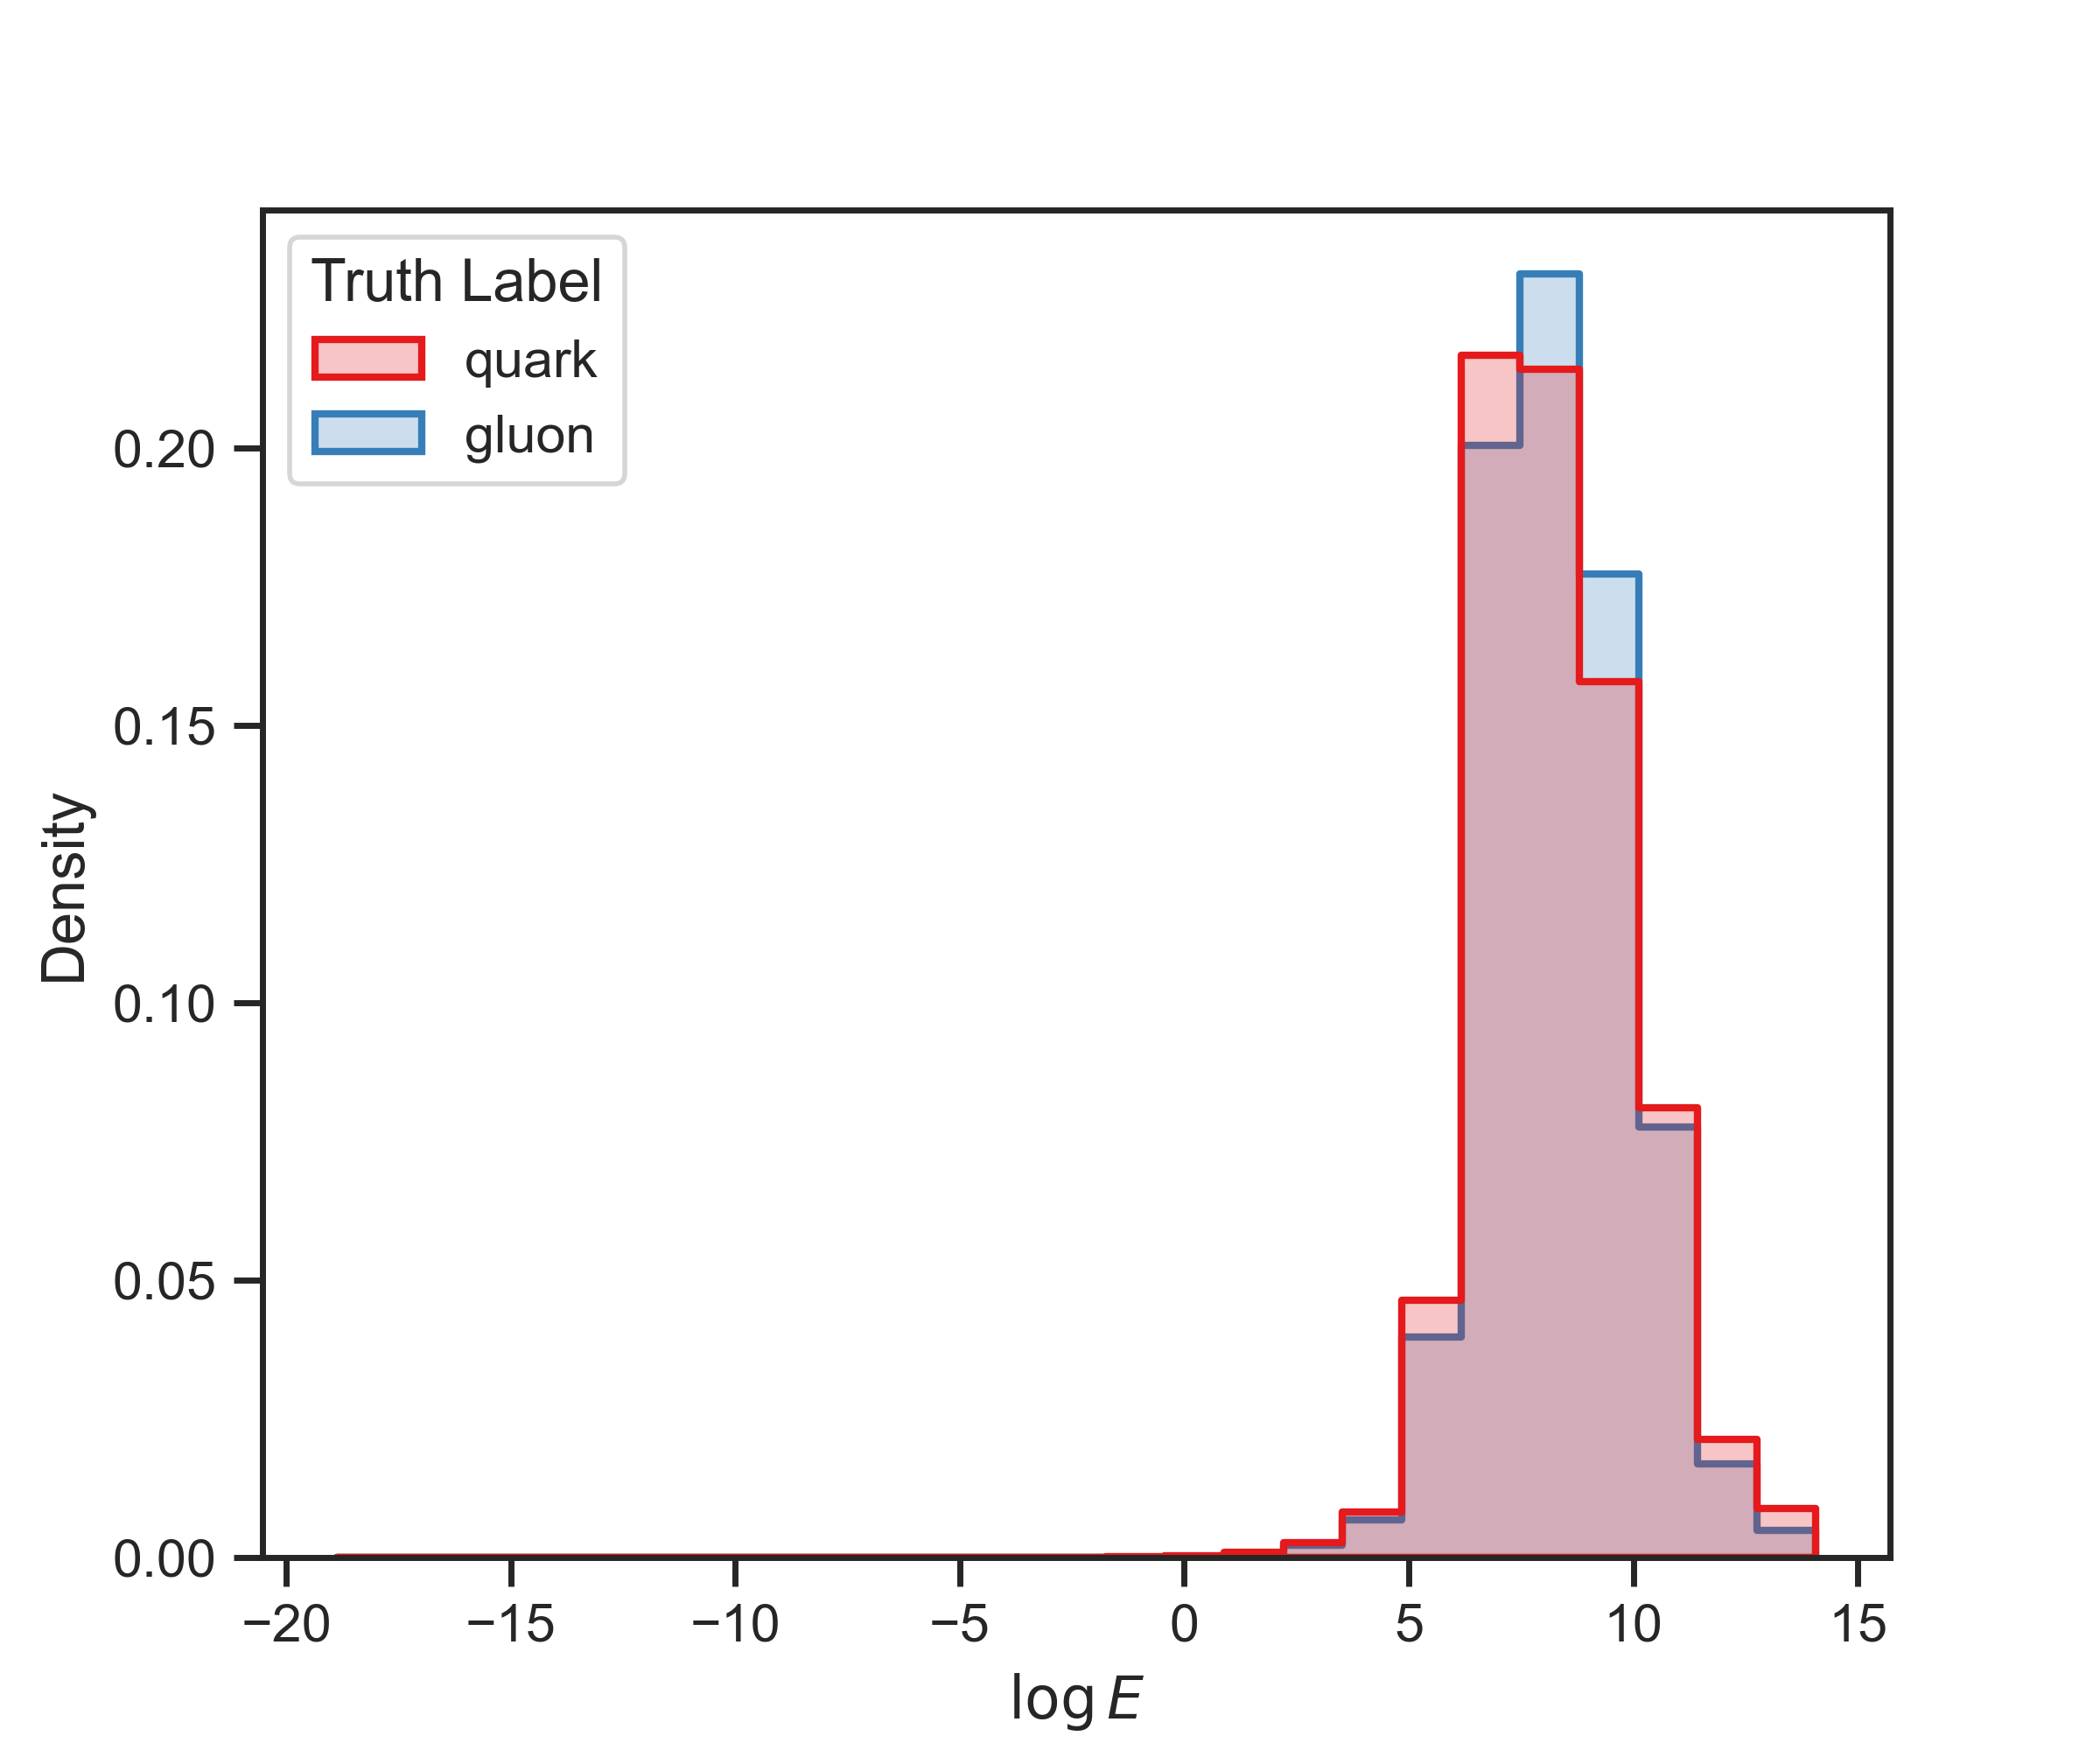
\includegraphics[width=\linewidth]{src/plots/distributions/PFOs/log_E.png}
        \caption{PFO $\log E$}
        \label{fig:app_pfo_log_E}
    \end{subfigure}
\caption{Distributions of PFO variables part 2.}
\label{fig:app_pfo_variables_2}
\end{figure}

\FloatBarrier
\newpage

\section{PFO Interaction Variables}
\label{sec:app_pfo_int_variables}

\begin{figure}[!htb]
    \begin{subfigure}[t]{0.45\textwidth}
        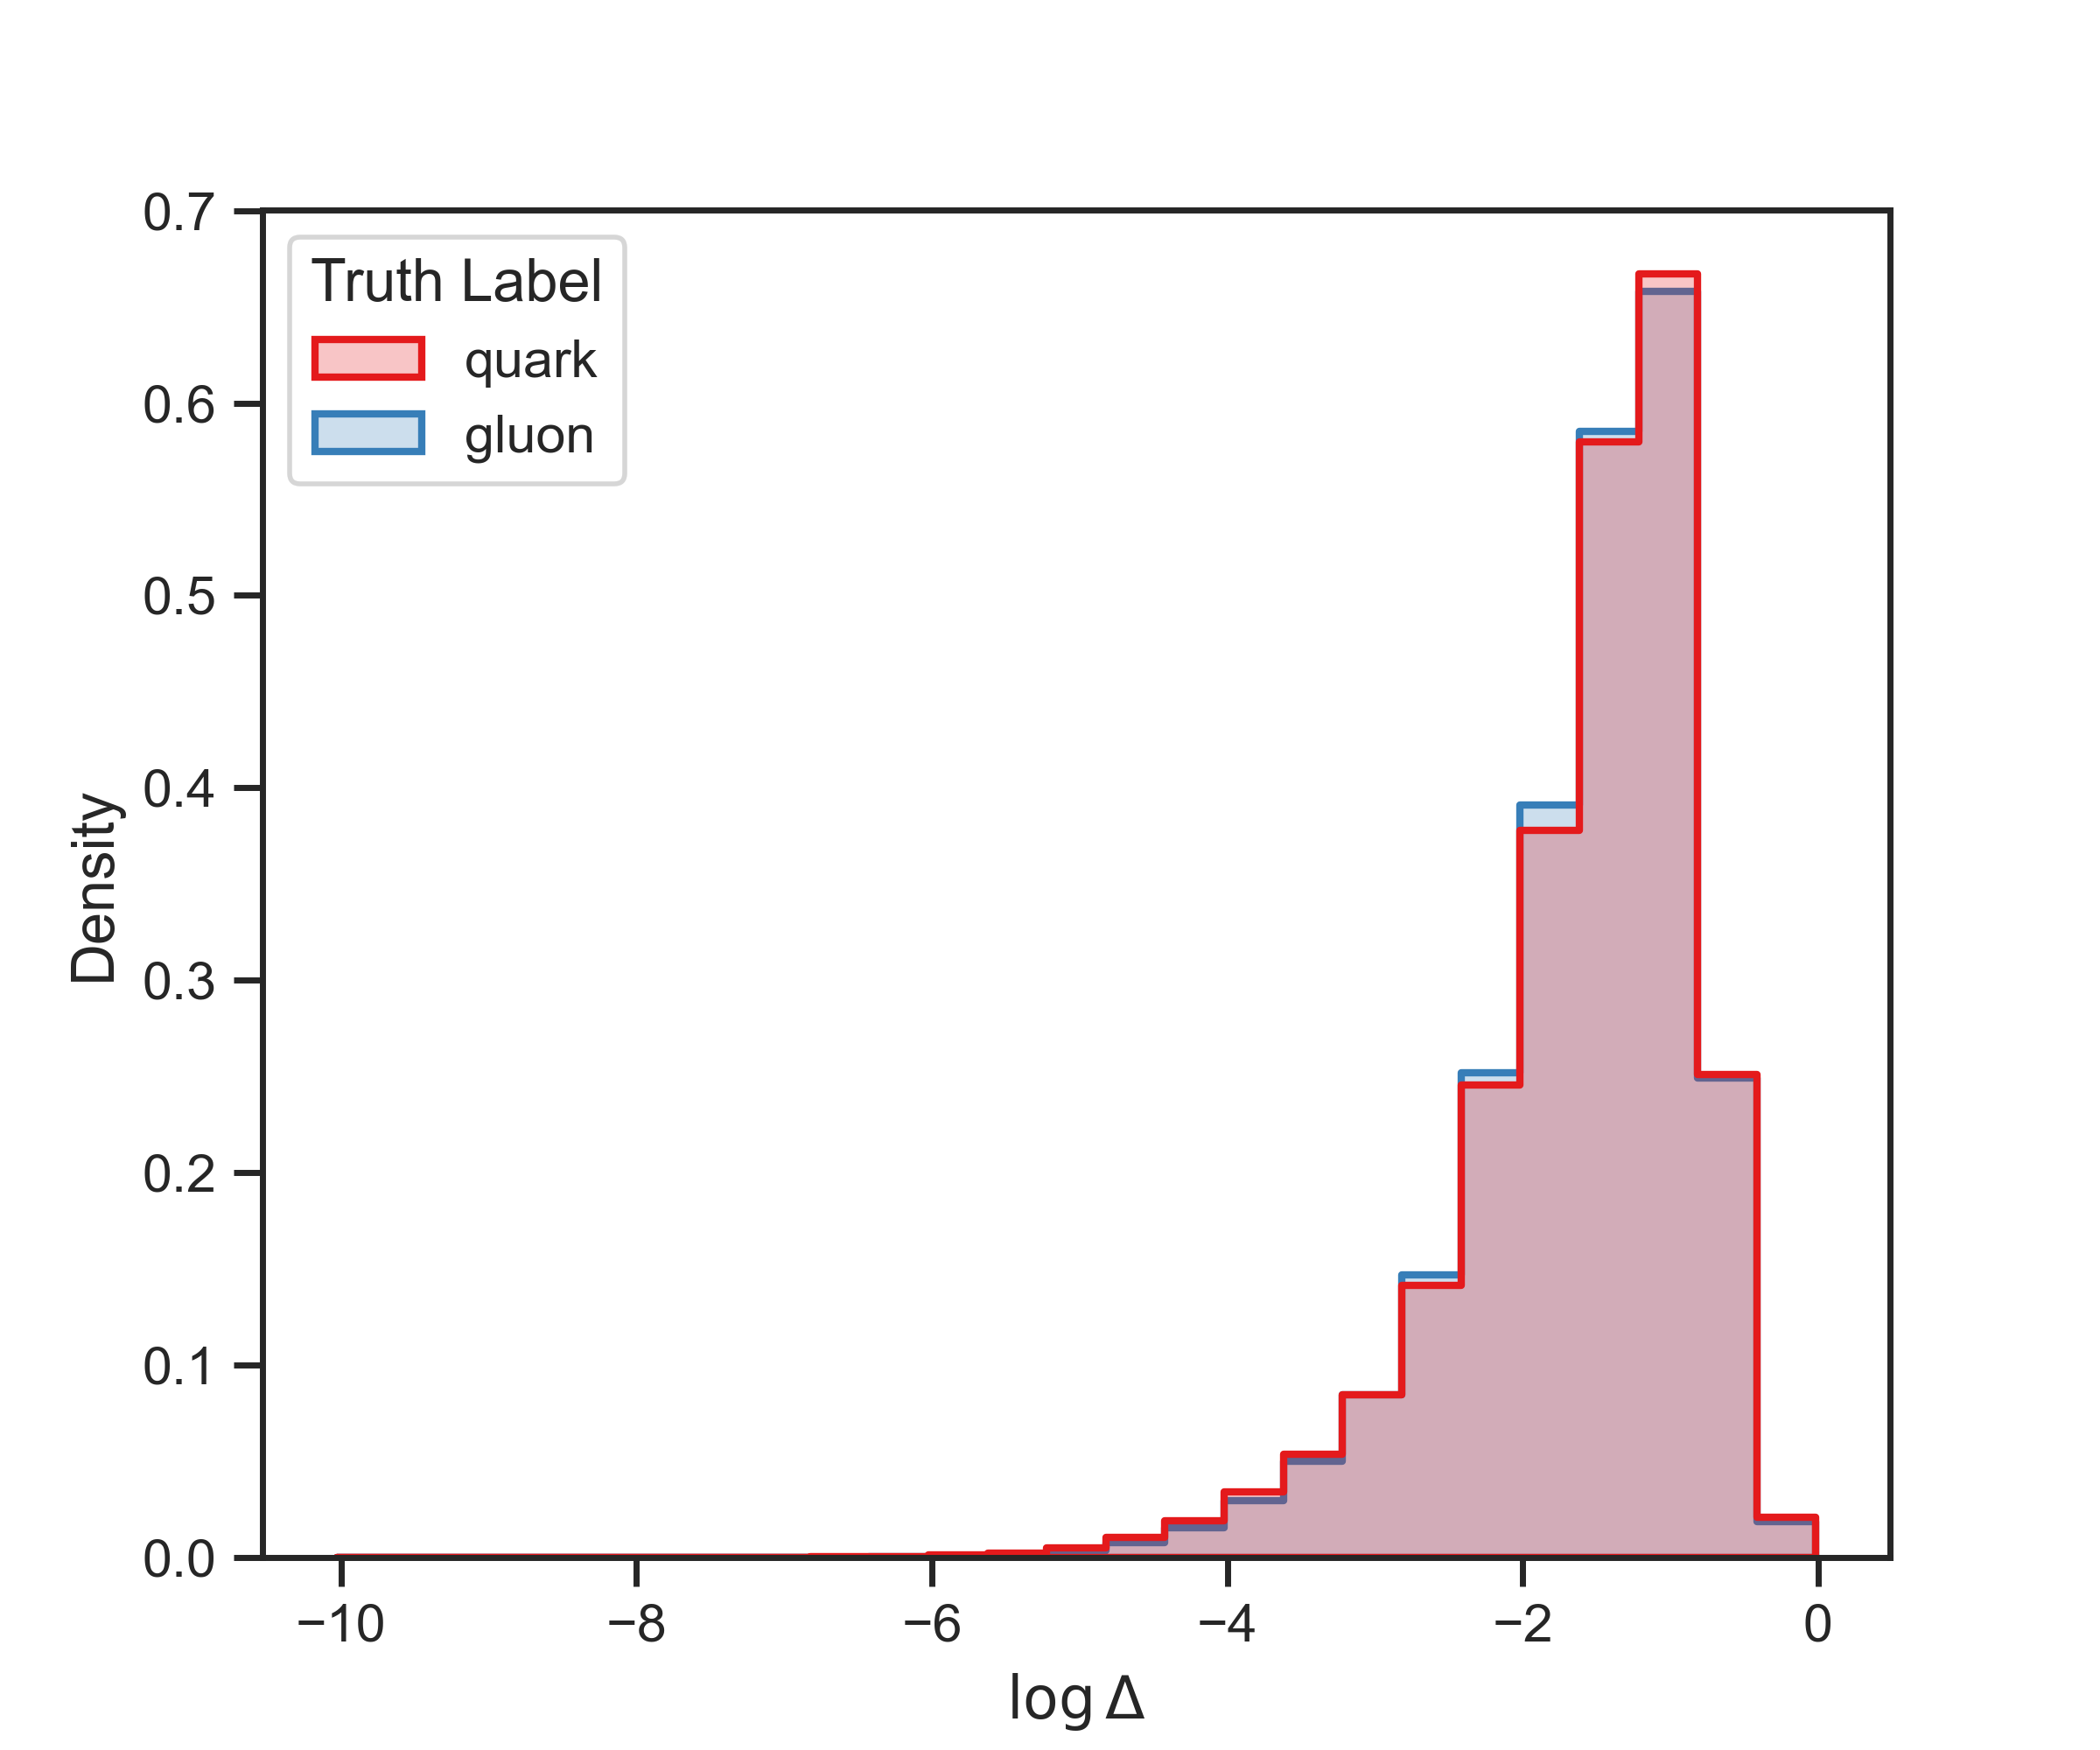
\includegraphics[width=\linewidth]{src/plots/distributions/int_PFOs/delta.png}
        \caption{PFO Interaction $\Delta$}
        \label{fig:app_pfo_interaction_delta}
    \end{subfigure}
    \begin{subfigure}[t]{0.45\textwidth}
        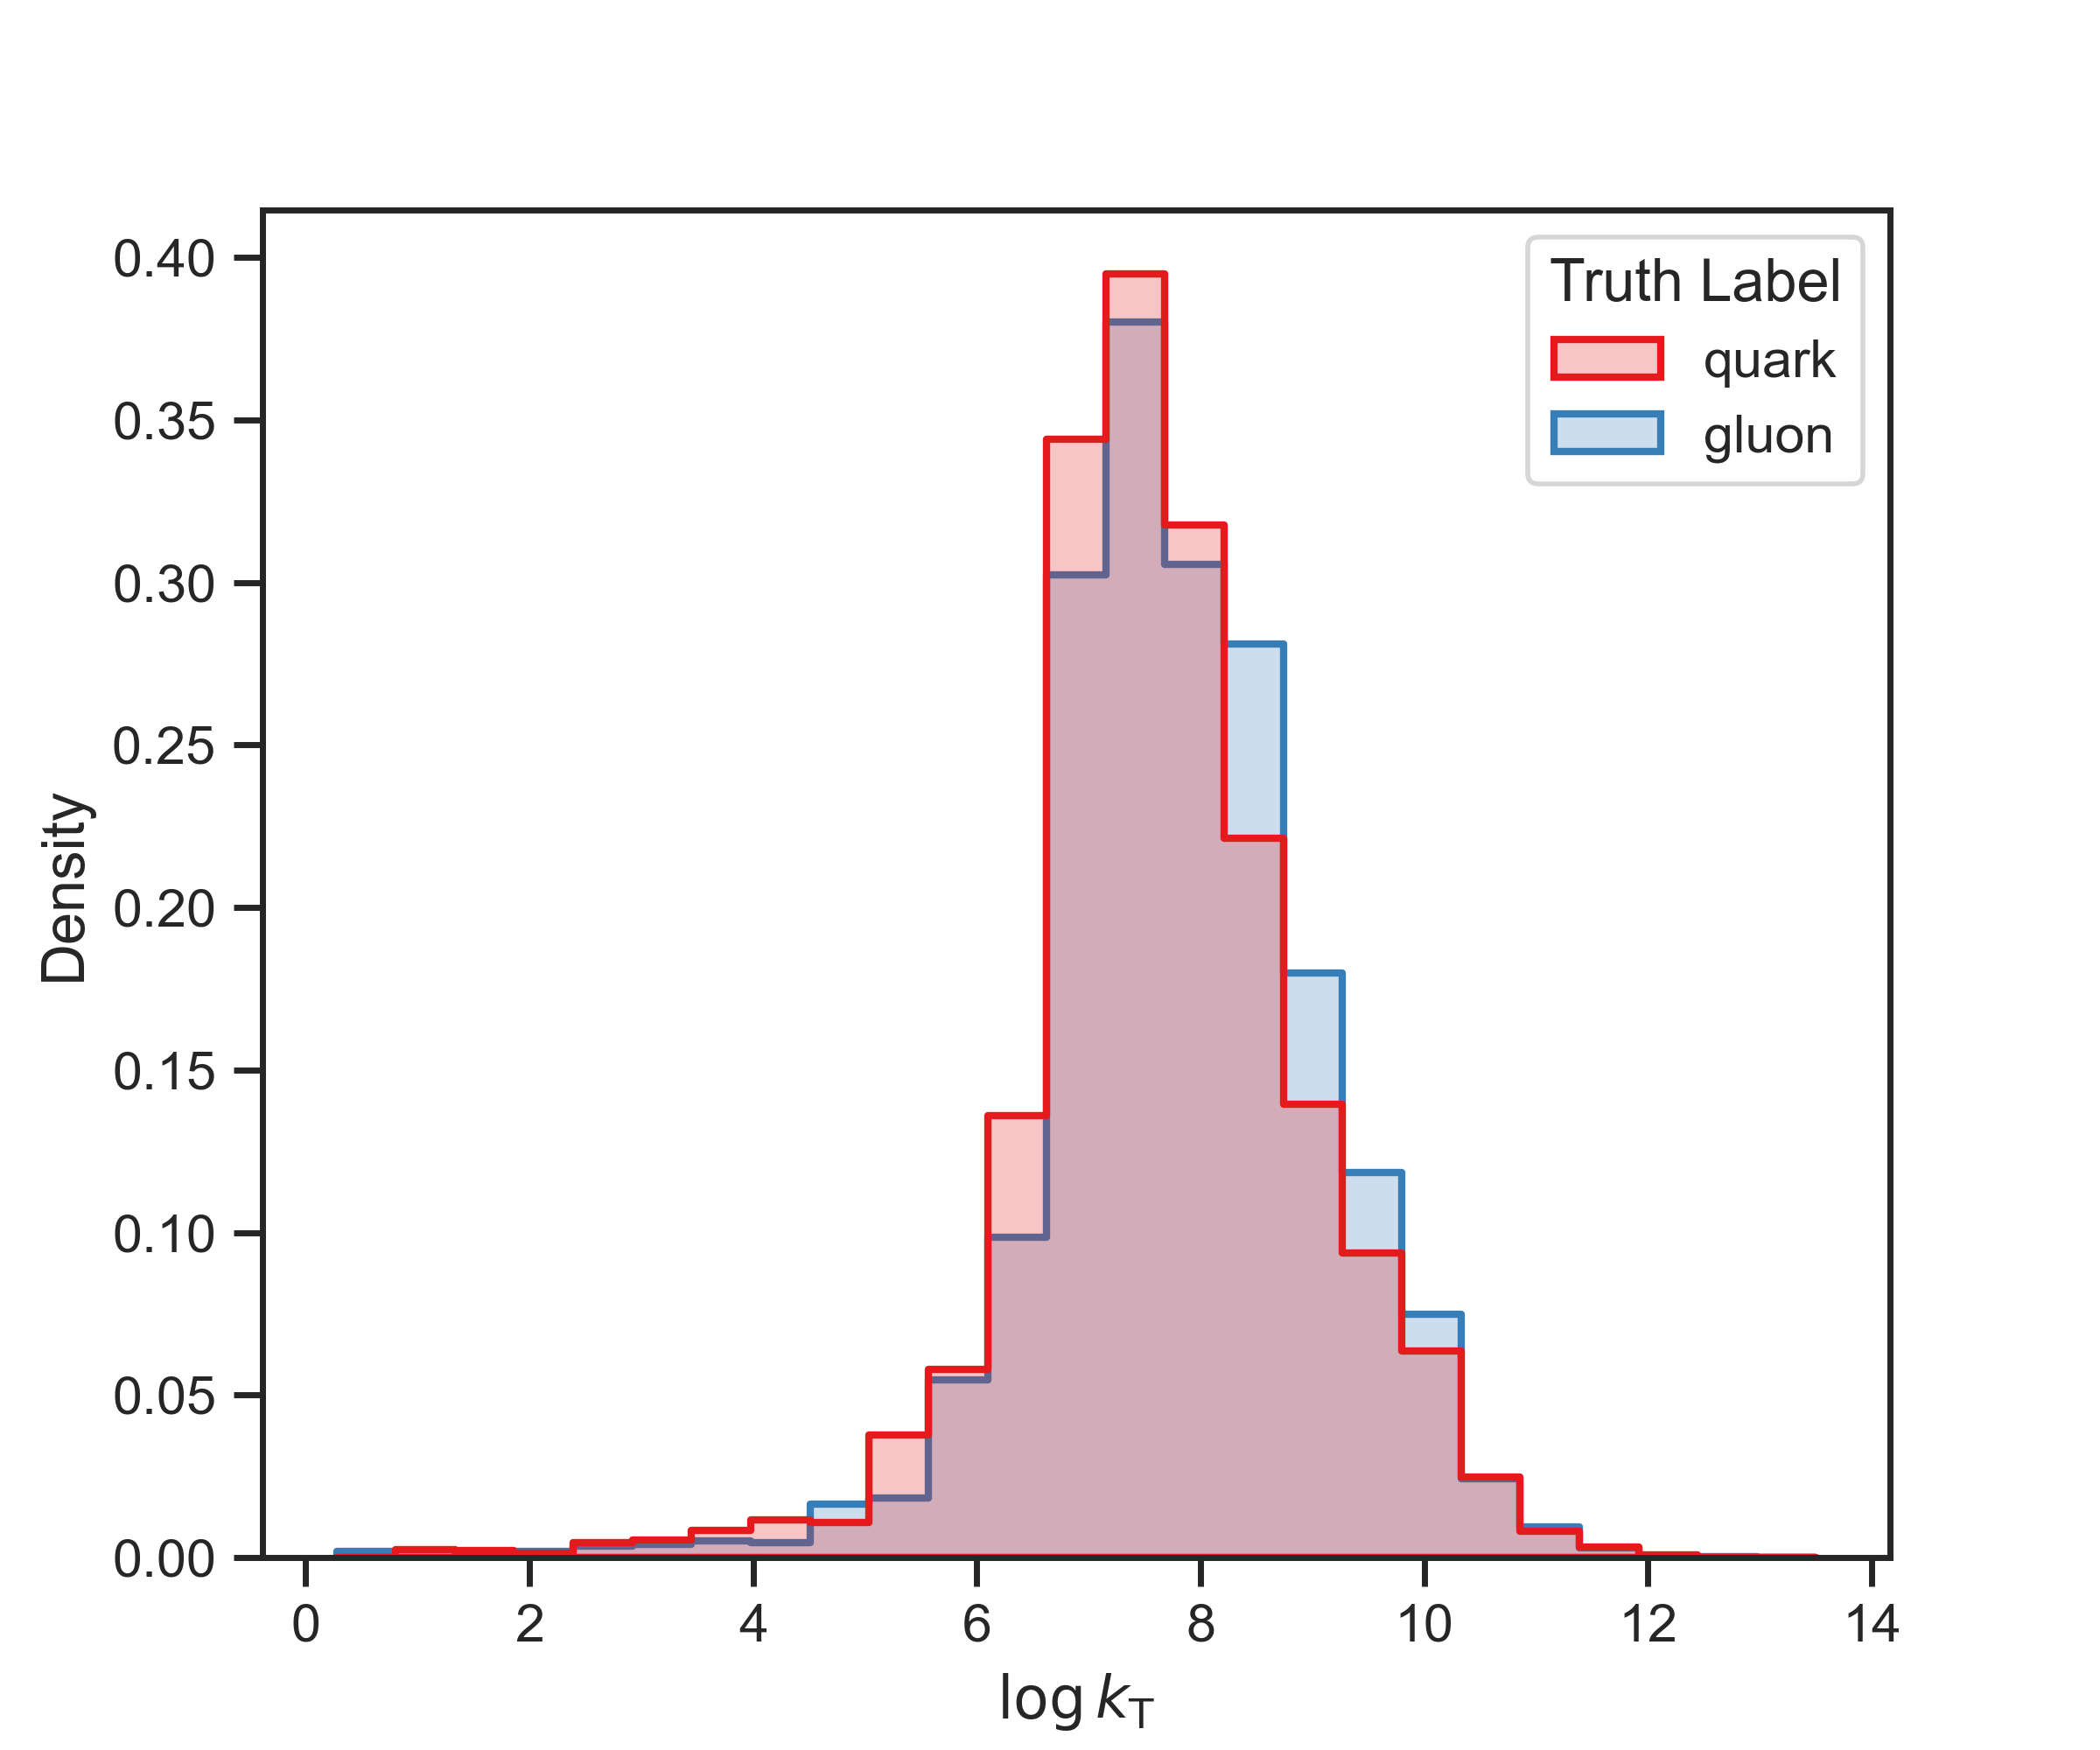
\includegraphics[width=\linewidth]{src/plots/distributions/int_PFOs/k_t.png}
        \caption{PFO Interaction $k_{\mathrm{T}}$}
        \label{fig:app_pfo_interaction_k_t}
    \end{subfigure}
    \begin{subfigure}[t]{0.45\textwidth}
        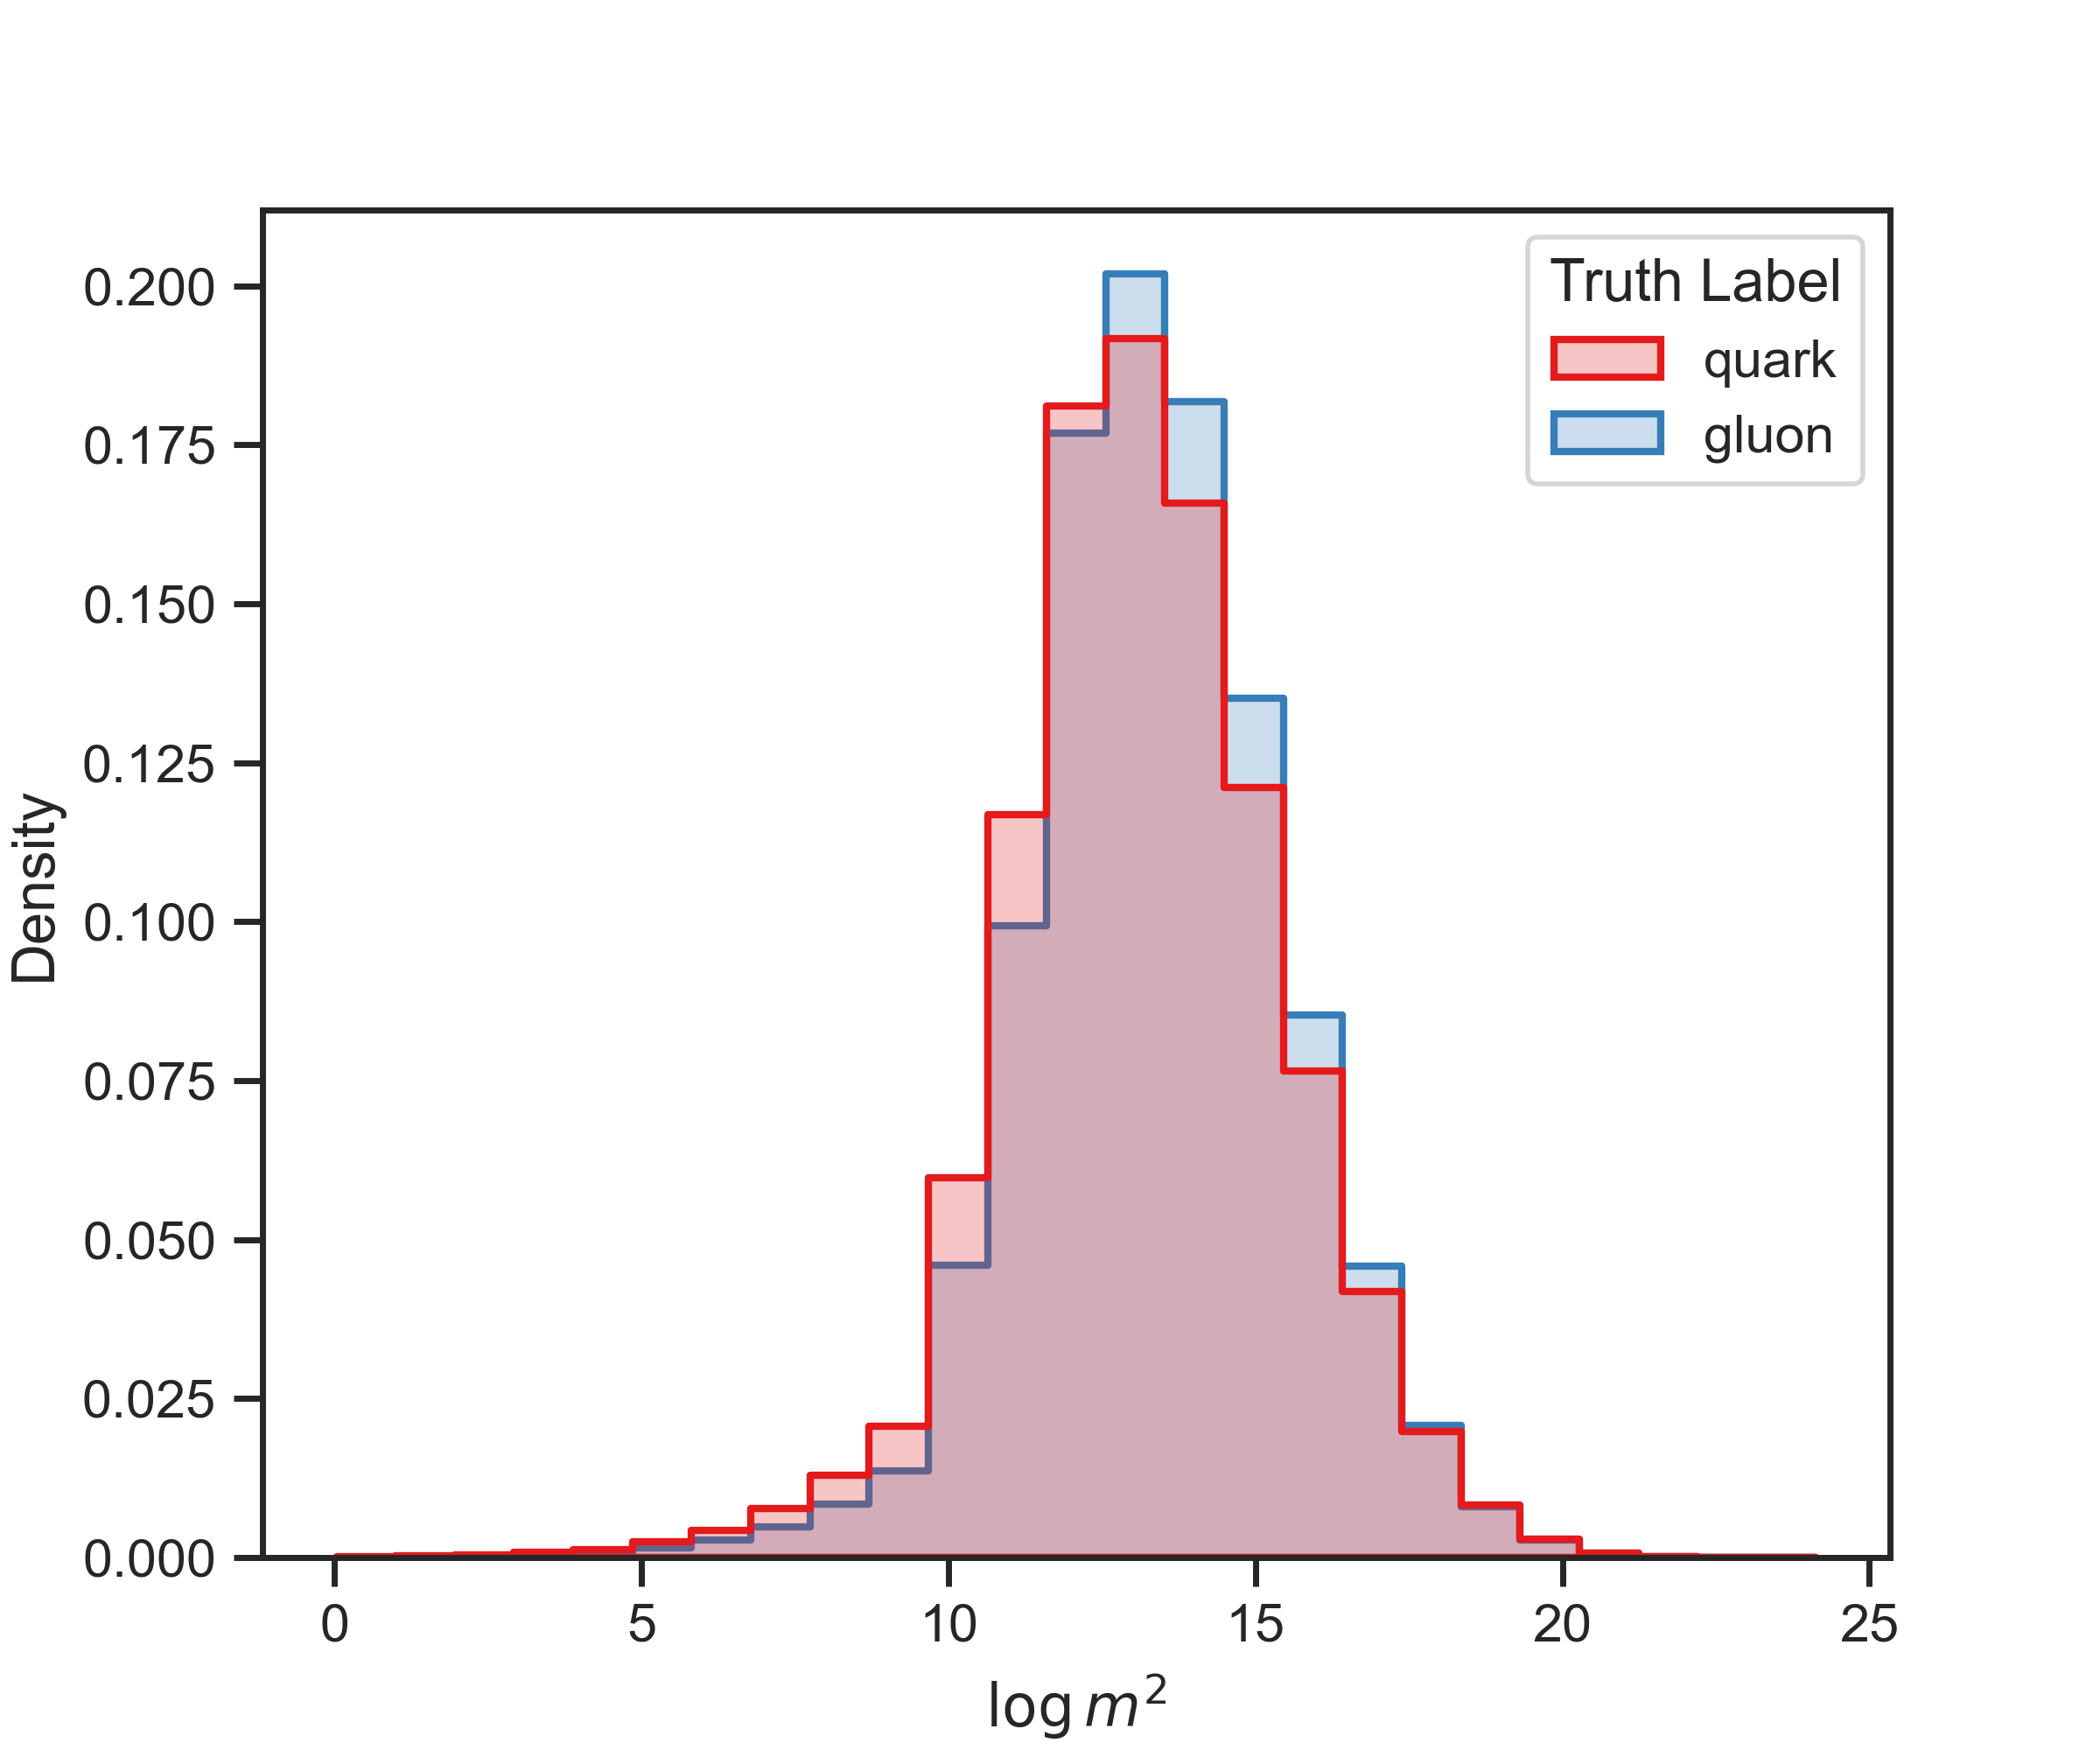
\includegraphics[width=\linewidth]{src/plots/distributions/int_PFOs/m2.png}
        \caption{PFO Interaction $m^2$}
        \label{fig:app_pfo_interaction_m2}
    \end{subfigure}
    \begin{subfigure}[t]{0.45\textwidth}
        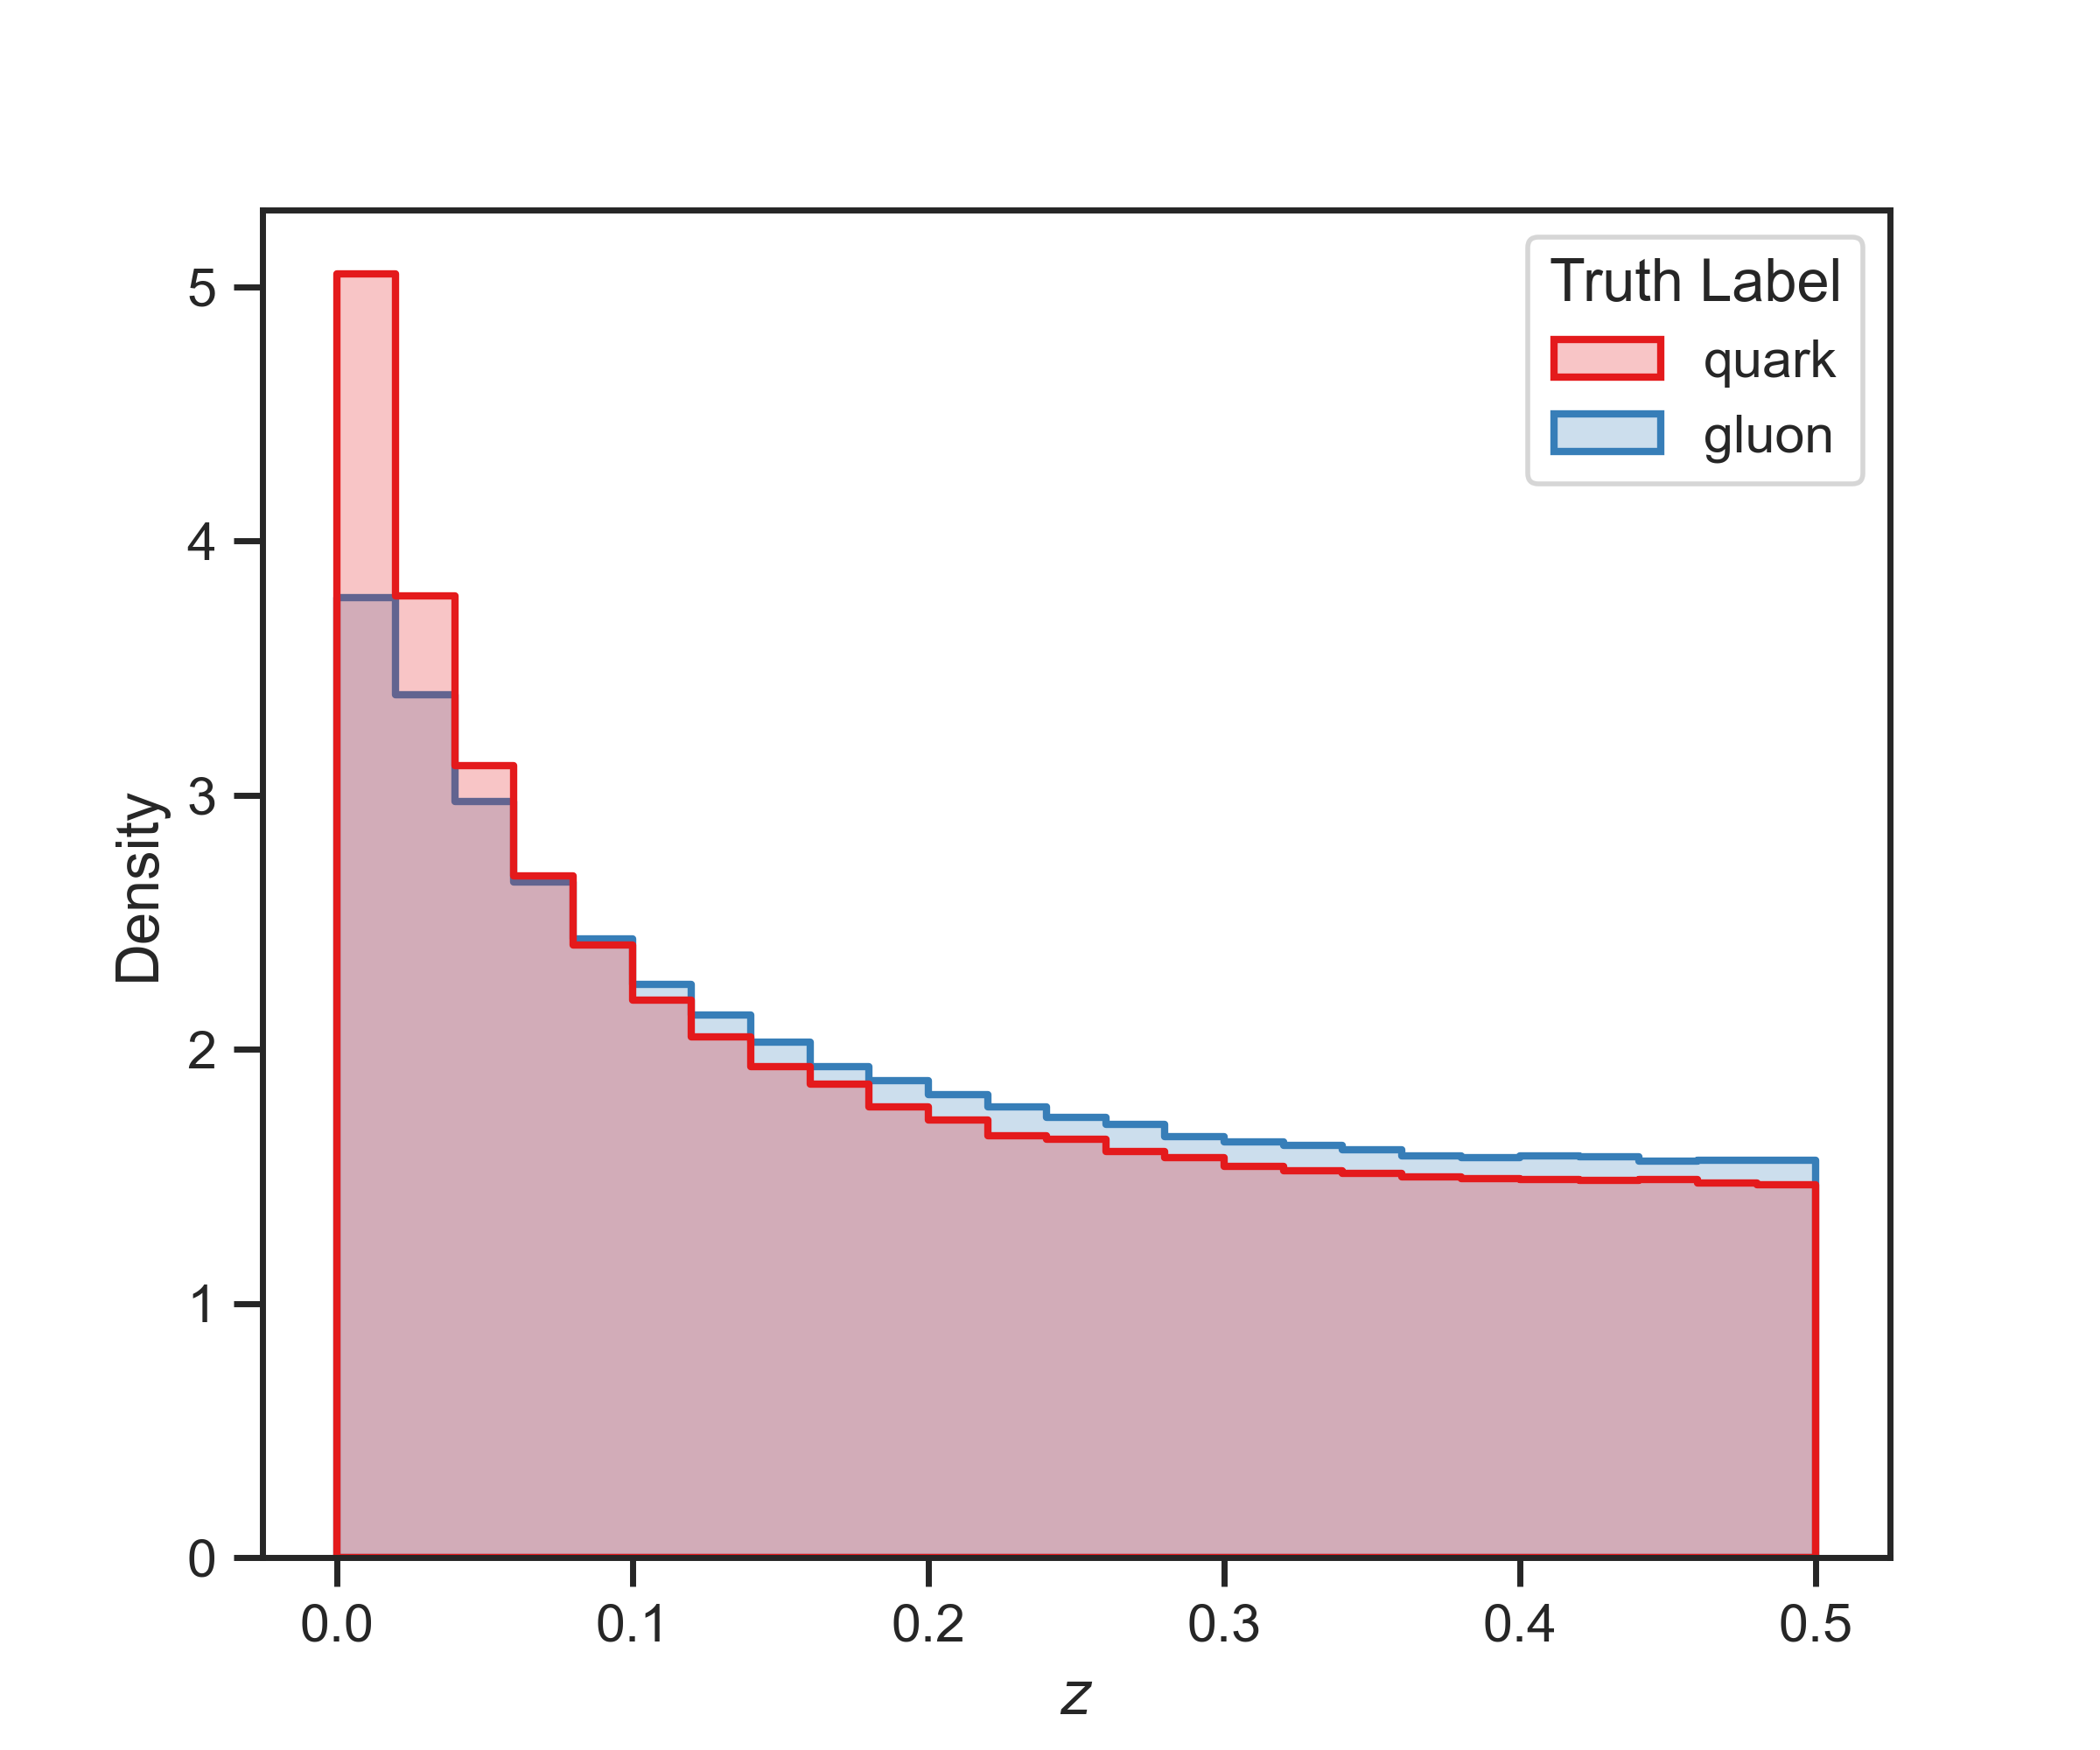
\includegraphics[width=\linewidth]{src/plots/distributions/int_PFOs/z.png}
        \caption{PFO Interaction $z$}
        \label{fig:app_pfo_interaction_z}
    \end{subfigure}
\caption{Distributions of PFO interaction variables.}
\label{fig:app_pfo_interaction_variables}
\end{figure}
\FloatBarrier
\newpage

\section{BDT Variables}
\label{sec:app_bdt_variables}
\begin{figure}[!htb]
    \centering
    \begin{subfigure}[t]{0.45\textwidth}
        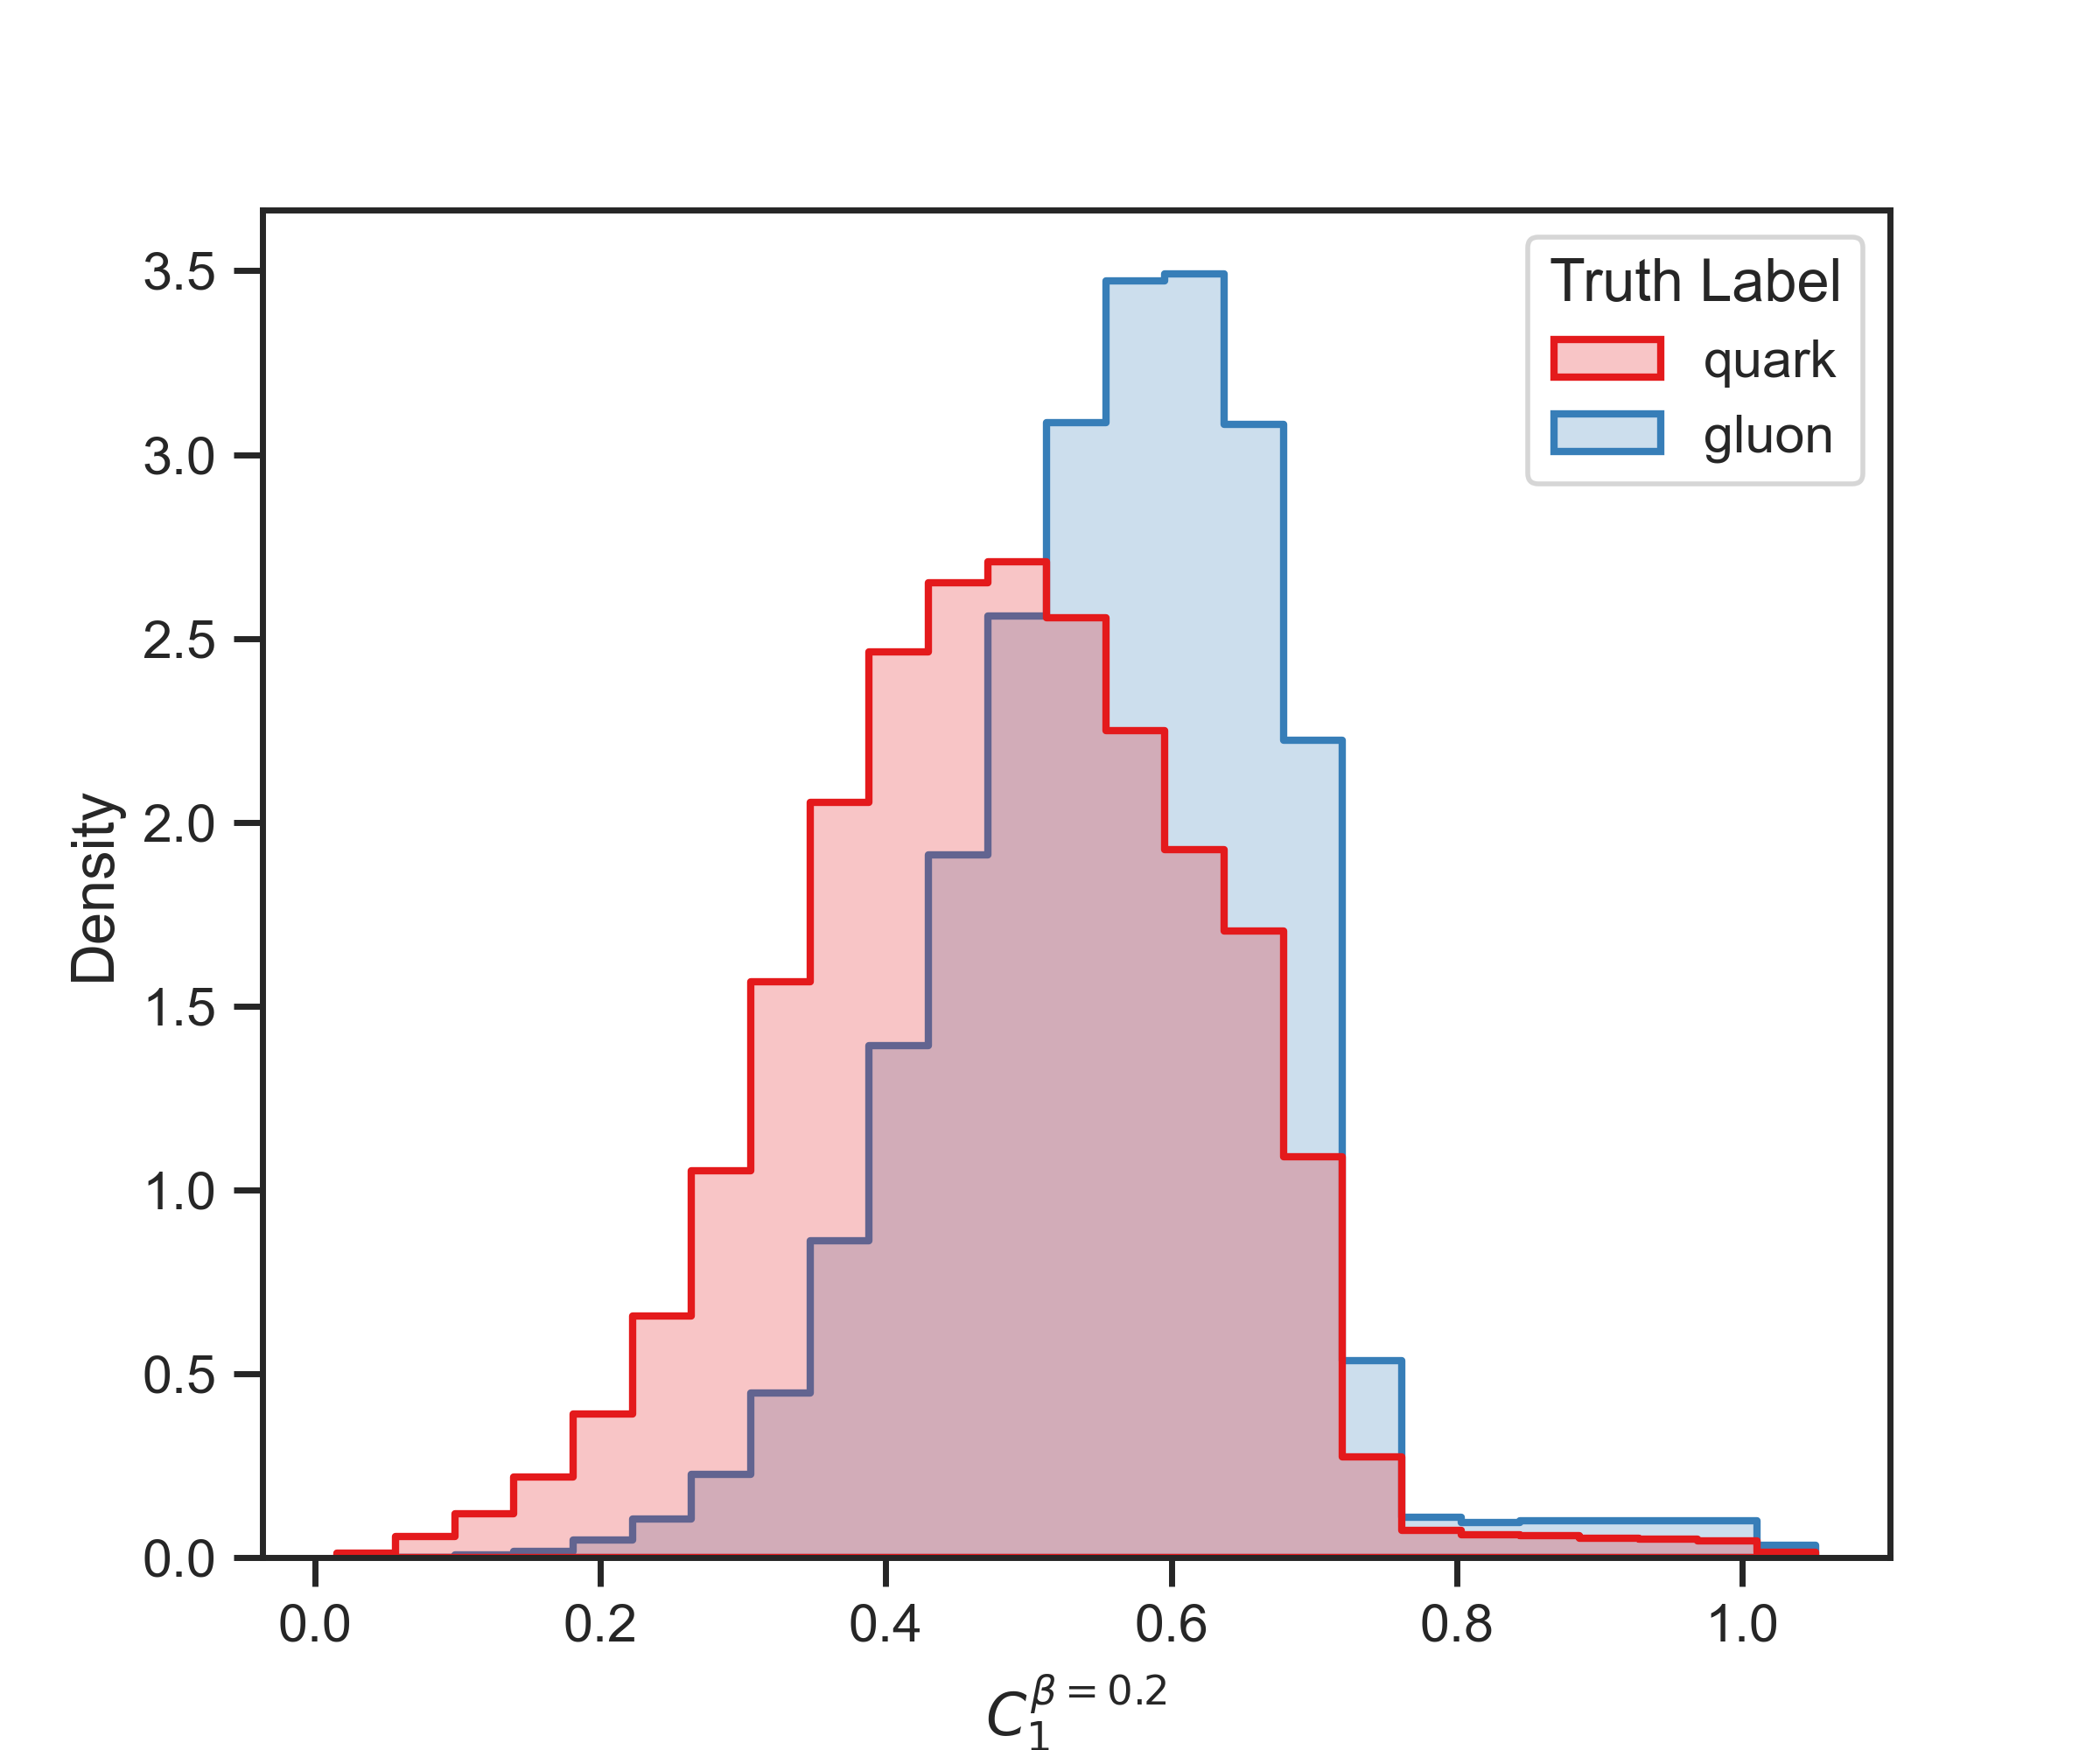
\includegraphics[width=\linewidth]{src/plots/distributions/BDT/C1_PFO_jet.png}
        \caption{BDT $C_1$}
        \label{fig:app_bdt_C1}
    \end{subfigure}
    \begin{subfigure}[t]{0.45\textwidth}
        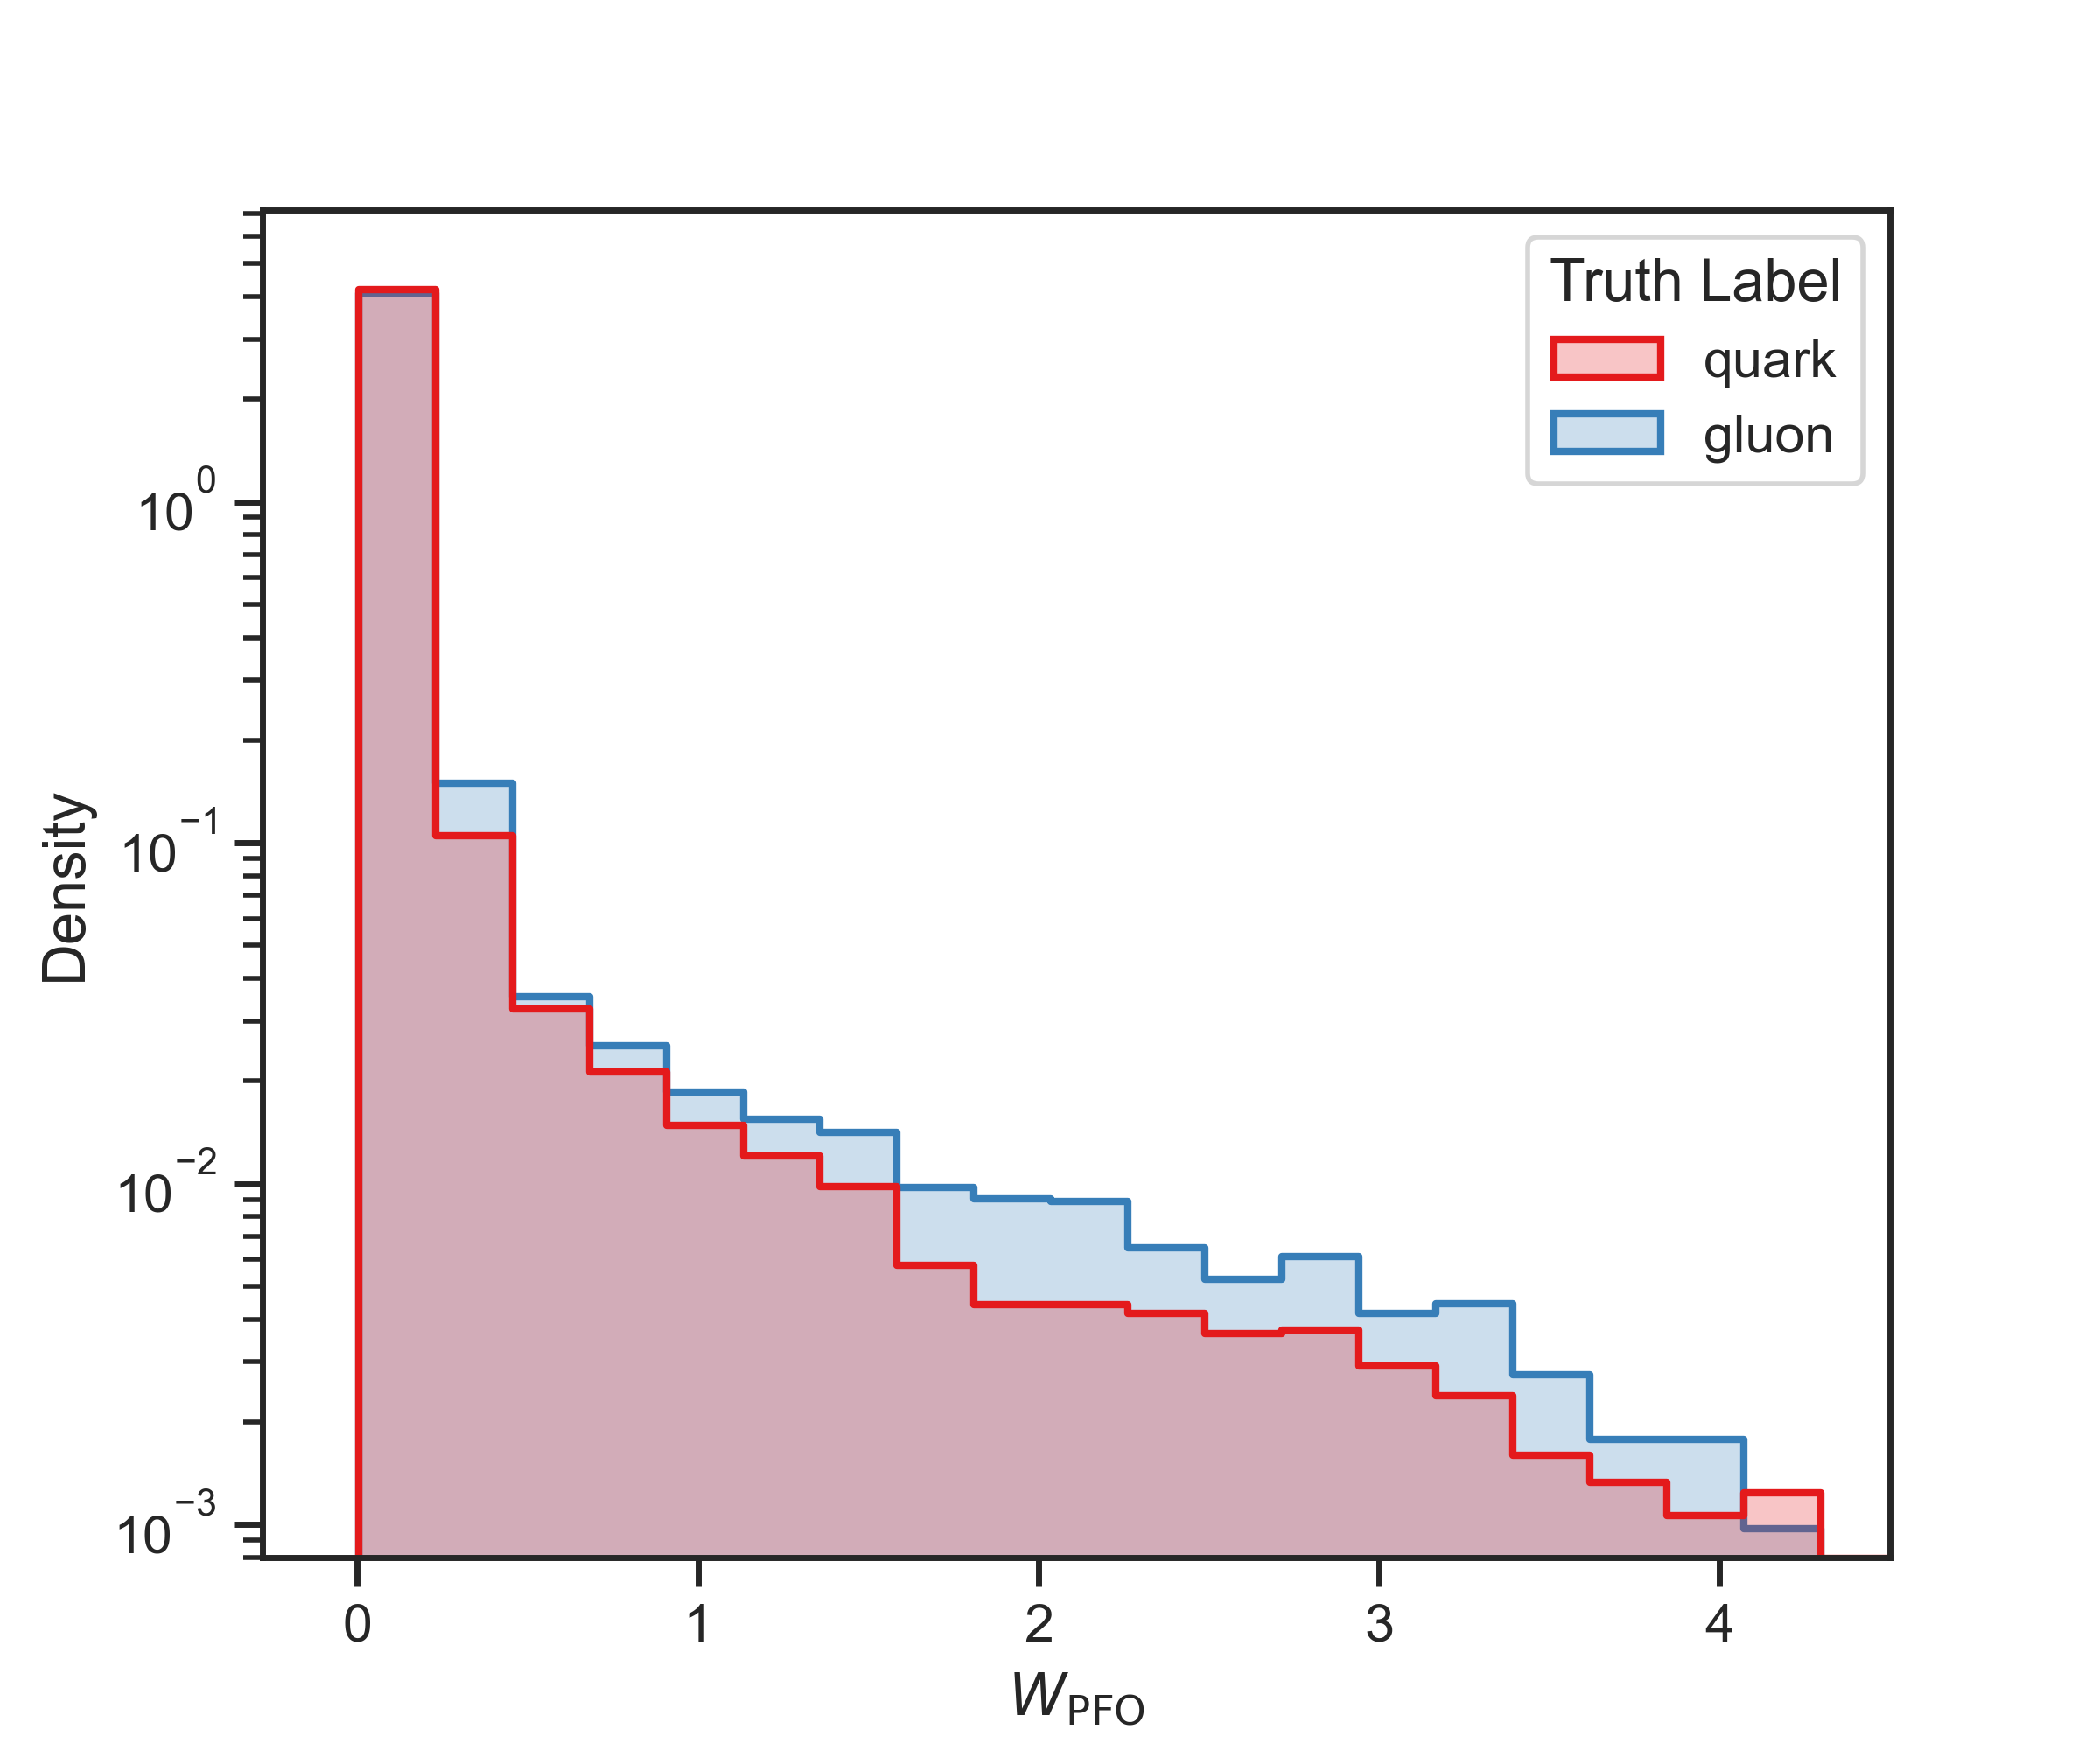
\includegraphics[width=\linewidth]{src/plots/distributions/BDT/W_PFO_jet.png}
        \caption{BDT $W_{\mathrm{PFO}}$}
        \label{fig:app_bdt_W_PFO}
    \end{subfigure}
    \begin{subfigure}[t]{0.45\textwidth}
        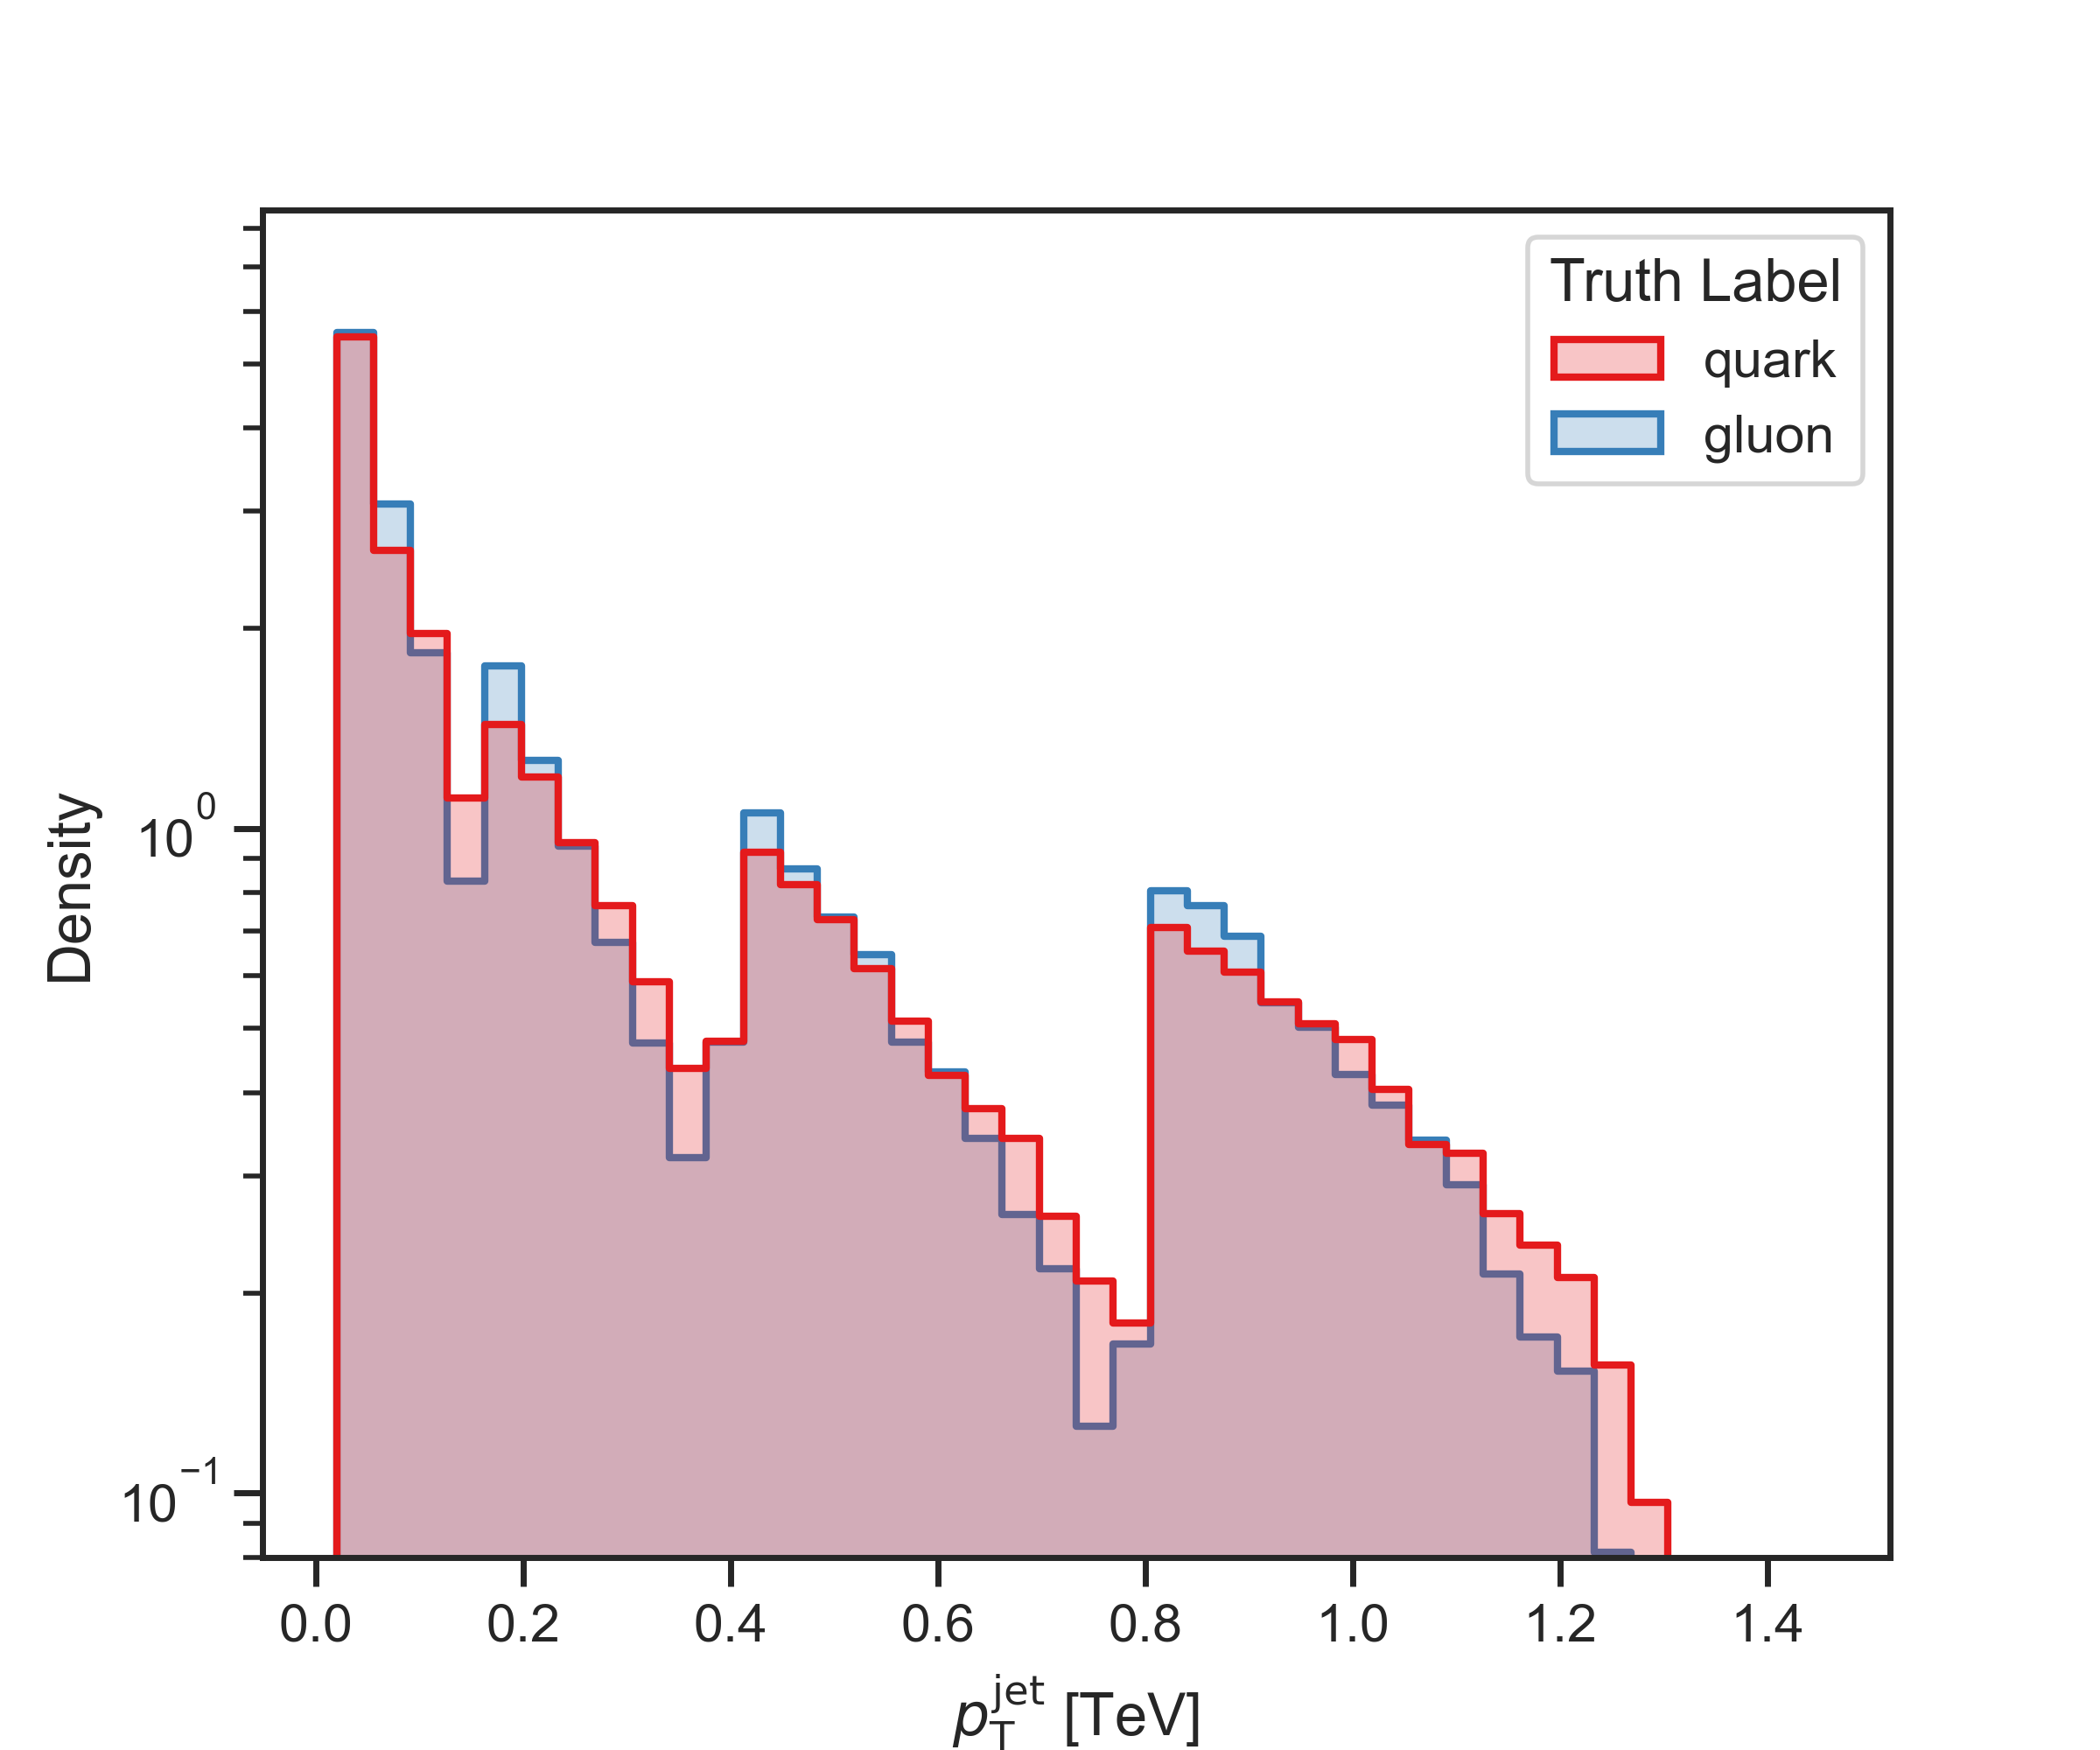
\includegraphics[width=\linewidth]{src/plots/distributions/BDT/pt_jet.png}
        \caption{BDT $p_{\mathrm{T}}^{\mathrm{jet}}$}
        \label{fig:app_bdt_pt_jet}
    \end{subfigure}
    \begin{subfigure}[t]{0.45\textwidth}
        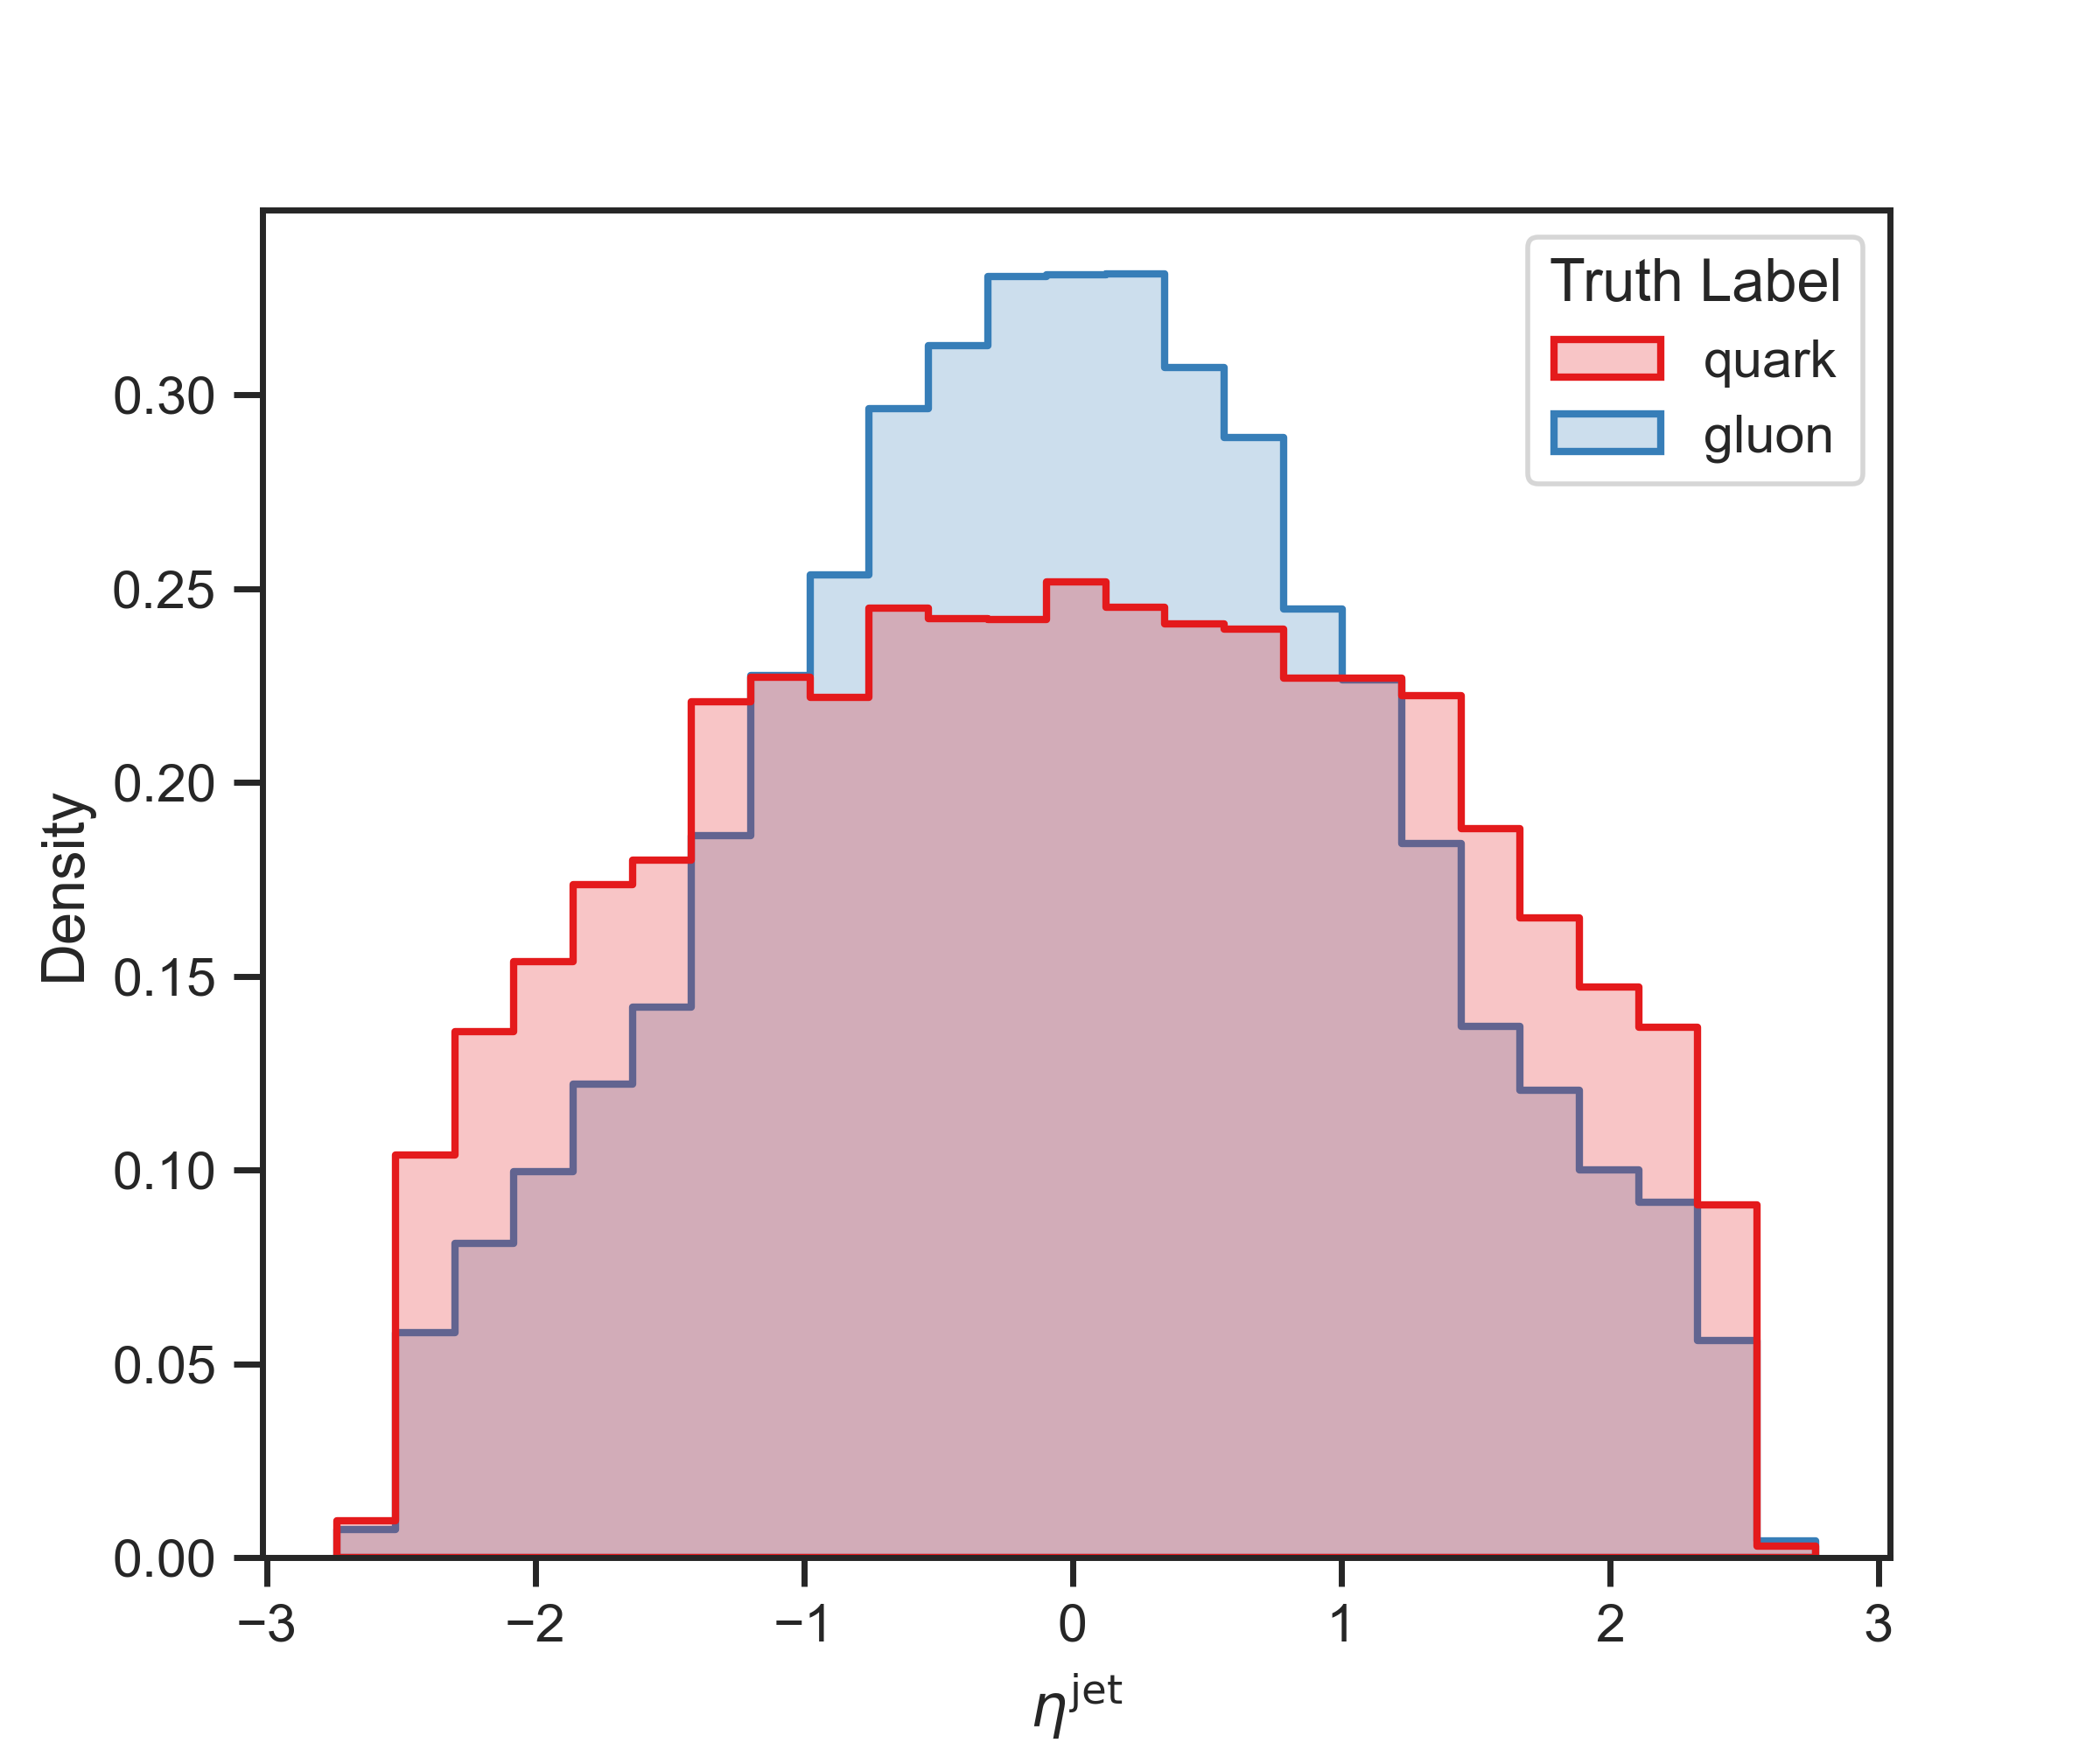
\includegraphics[width=\linewidth]{src/plots/distributions/BDT/eta_jet.png}
        \caption{BDT $\eta^{\mathrm{jet}}$}
        \label{fig:app_bdt_eta_jet}
    \end{subfigure}
    \begin{subfigure}[t]{0.45\textwidth}
        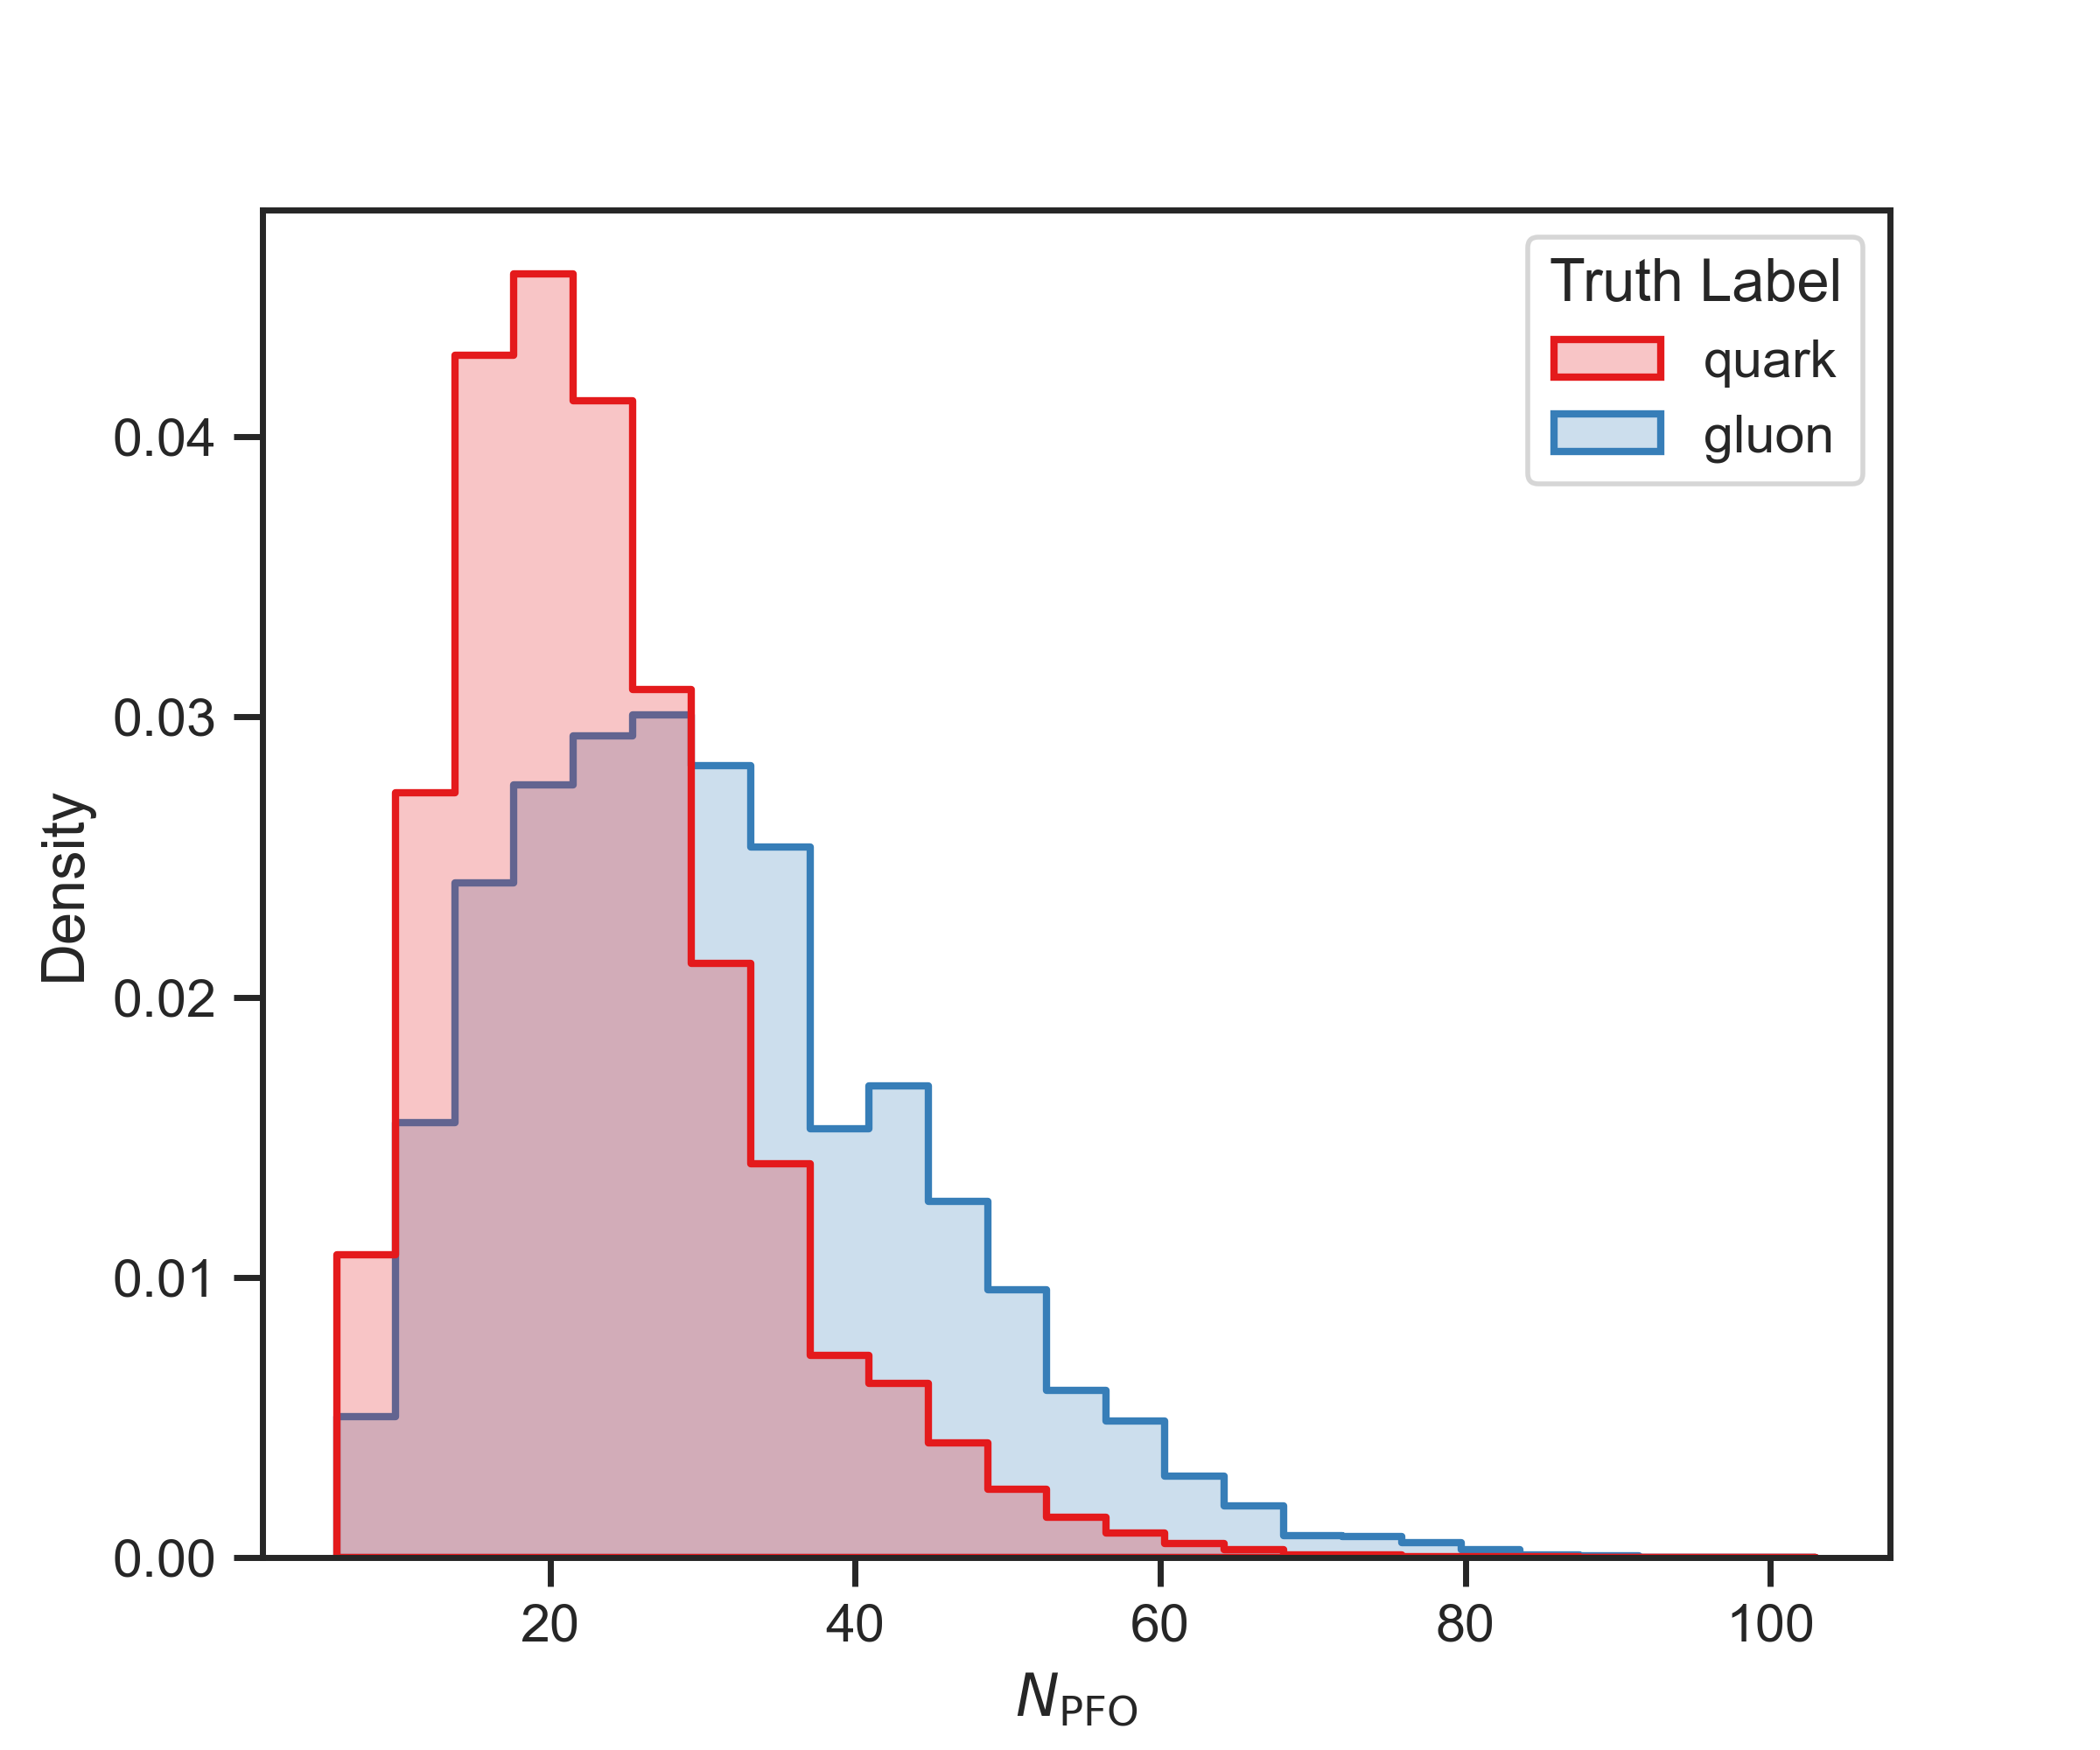
\includegraphics[width=\linewidth]{src/plots/distributions/BDT/N_PFO.png}
        \caption{BDT $N_{\mathrm{PFO}}$}
        \label{fig:app_bdt_N_PFO}
    \end{subfigure}
\caption{Distributions of BDT variables.}
\label{fig:app_bdt_variables}
\end{figure}

\FloatBarrier
\newpage

\section{High-level Jet Variables}
\label{sec:app_high_level_variables}

\begin{figure}[!htb]
	\centering
	\begin{subfigure}[t]{0.48\textwidth}
		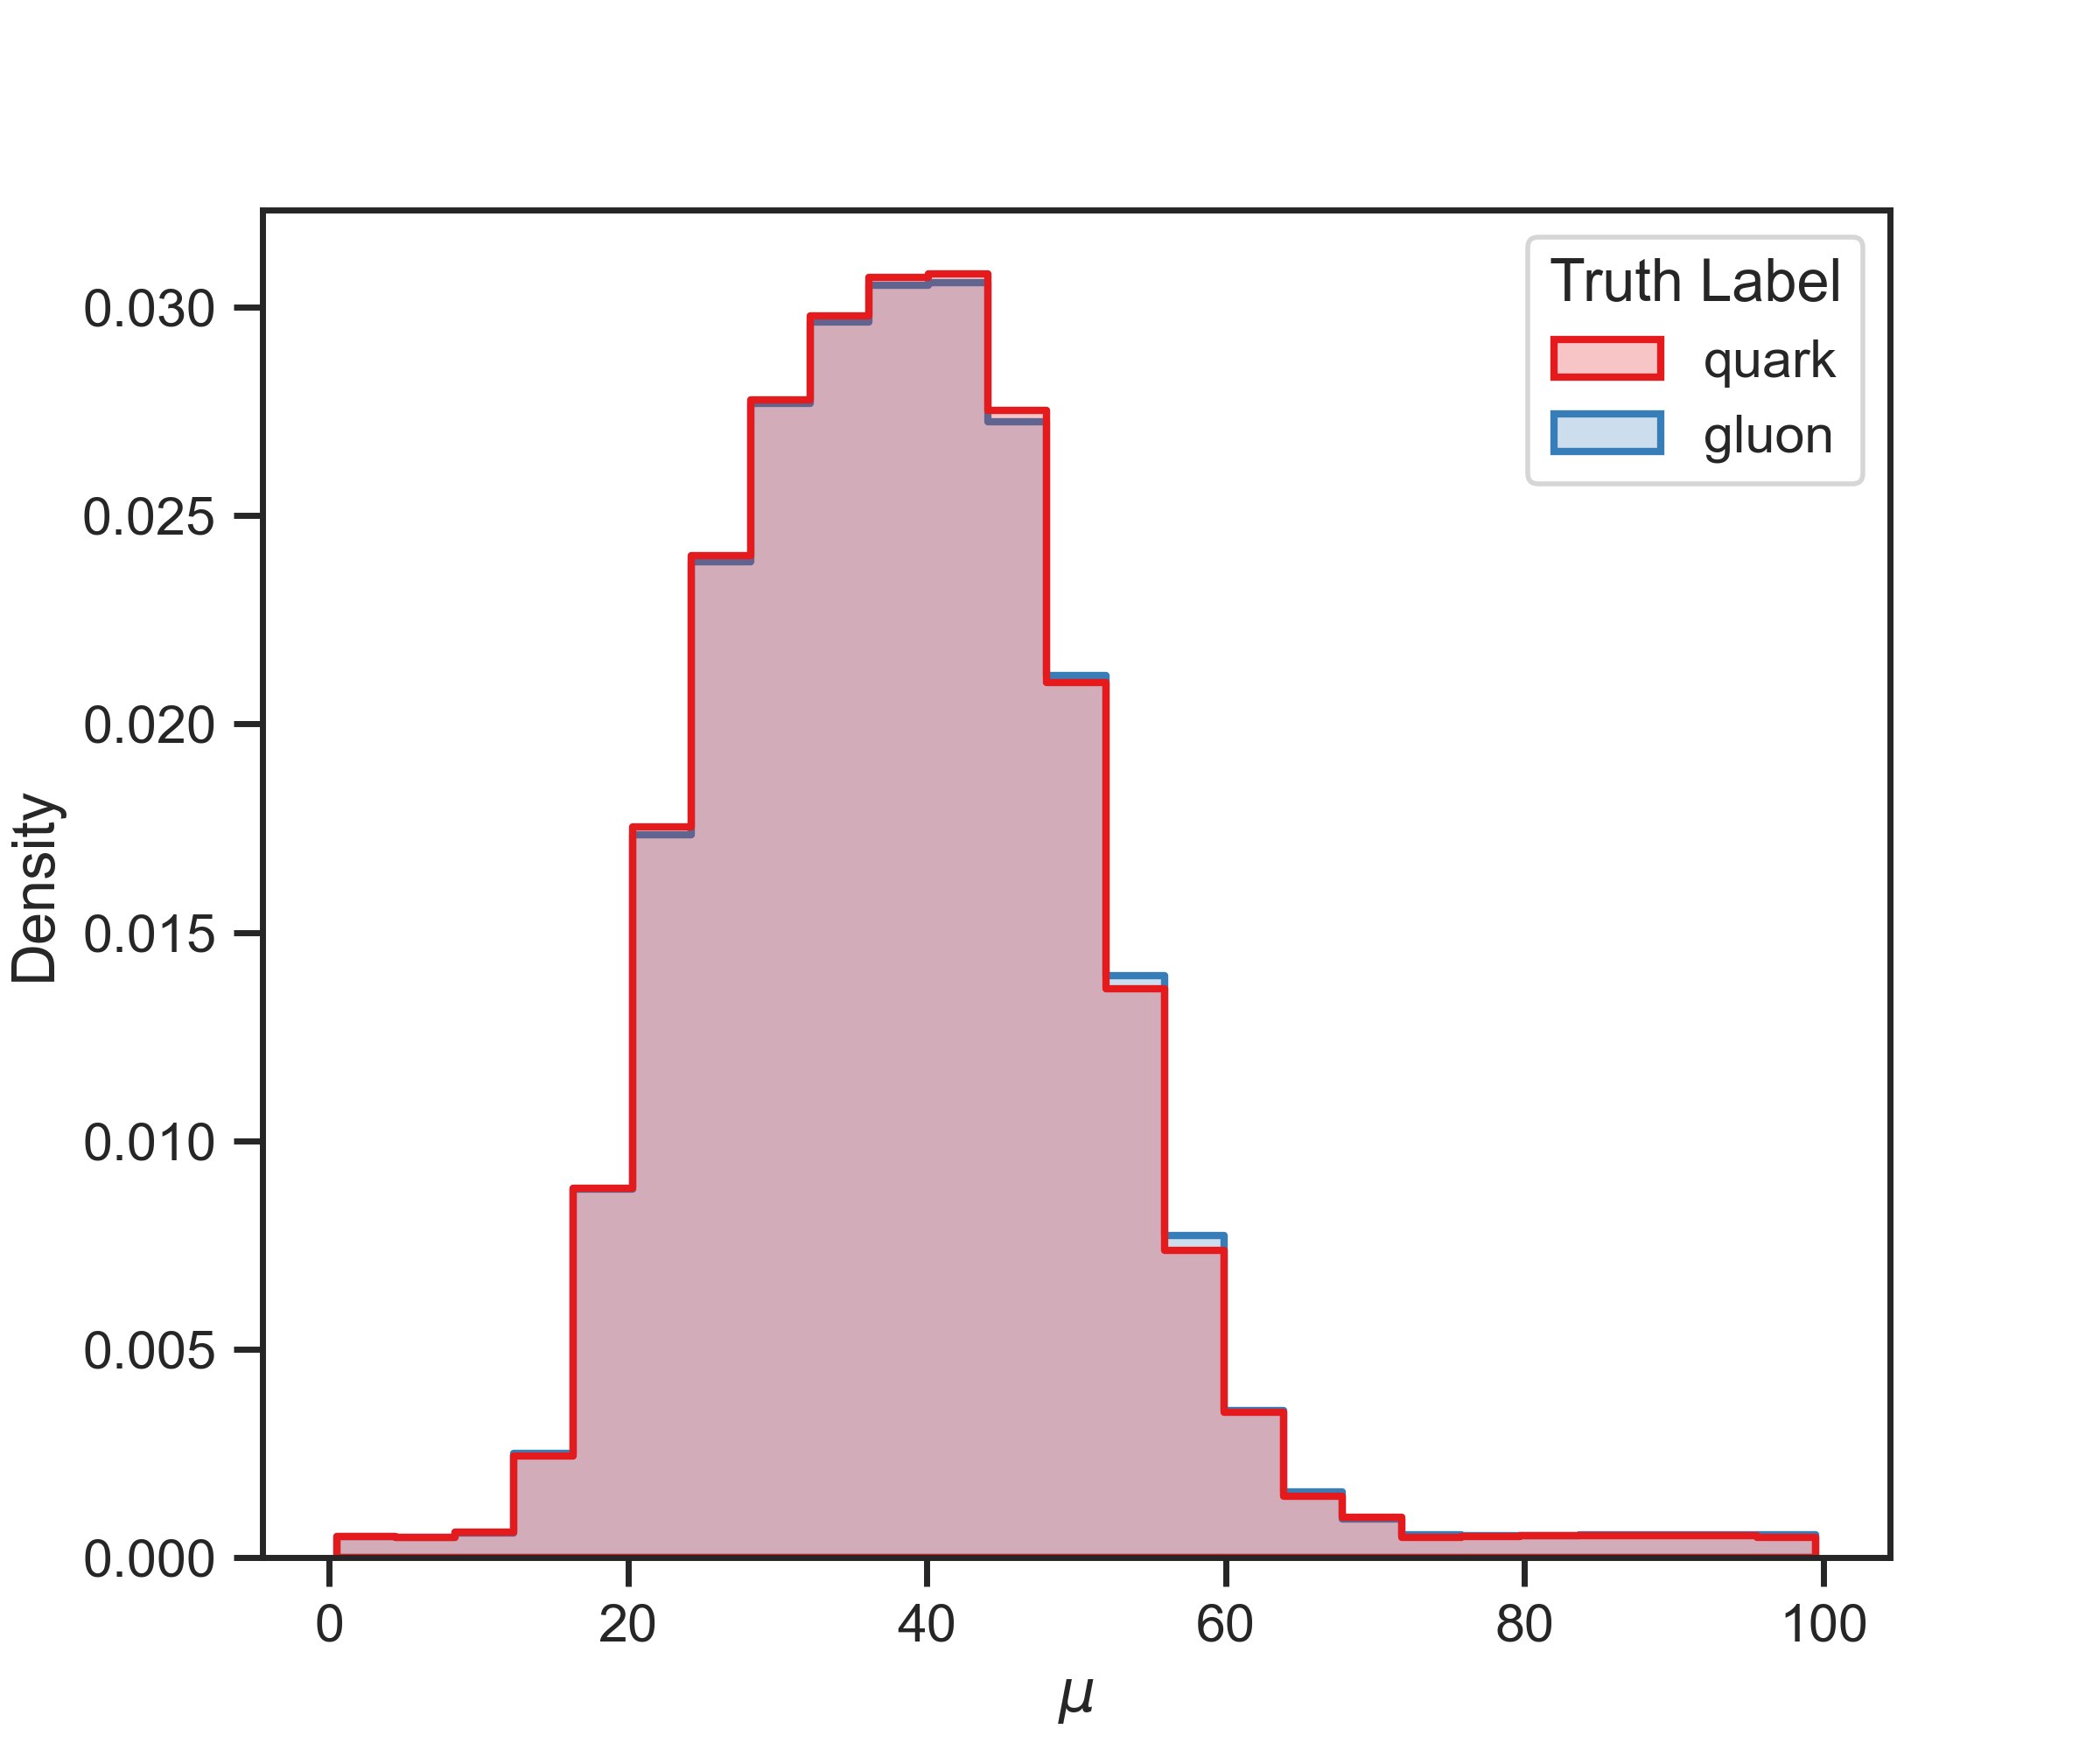
\includegraphics[width=1\textwidth]{src/plots/distributions/highlevel/corrected_averageInteractionsPerCrossing[0].png}
		\caption{\texttt{averageInteractionsPerCrossing[0]}}
		\label{fig:highlevel_0}
	\end{subfigure}
	\begin{subfigure}[t]{0.48\textwidth}
		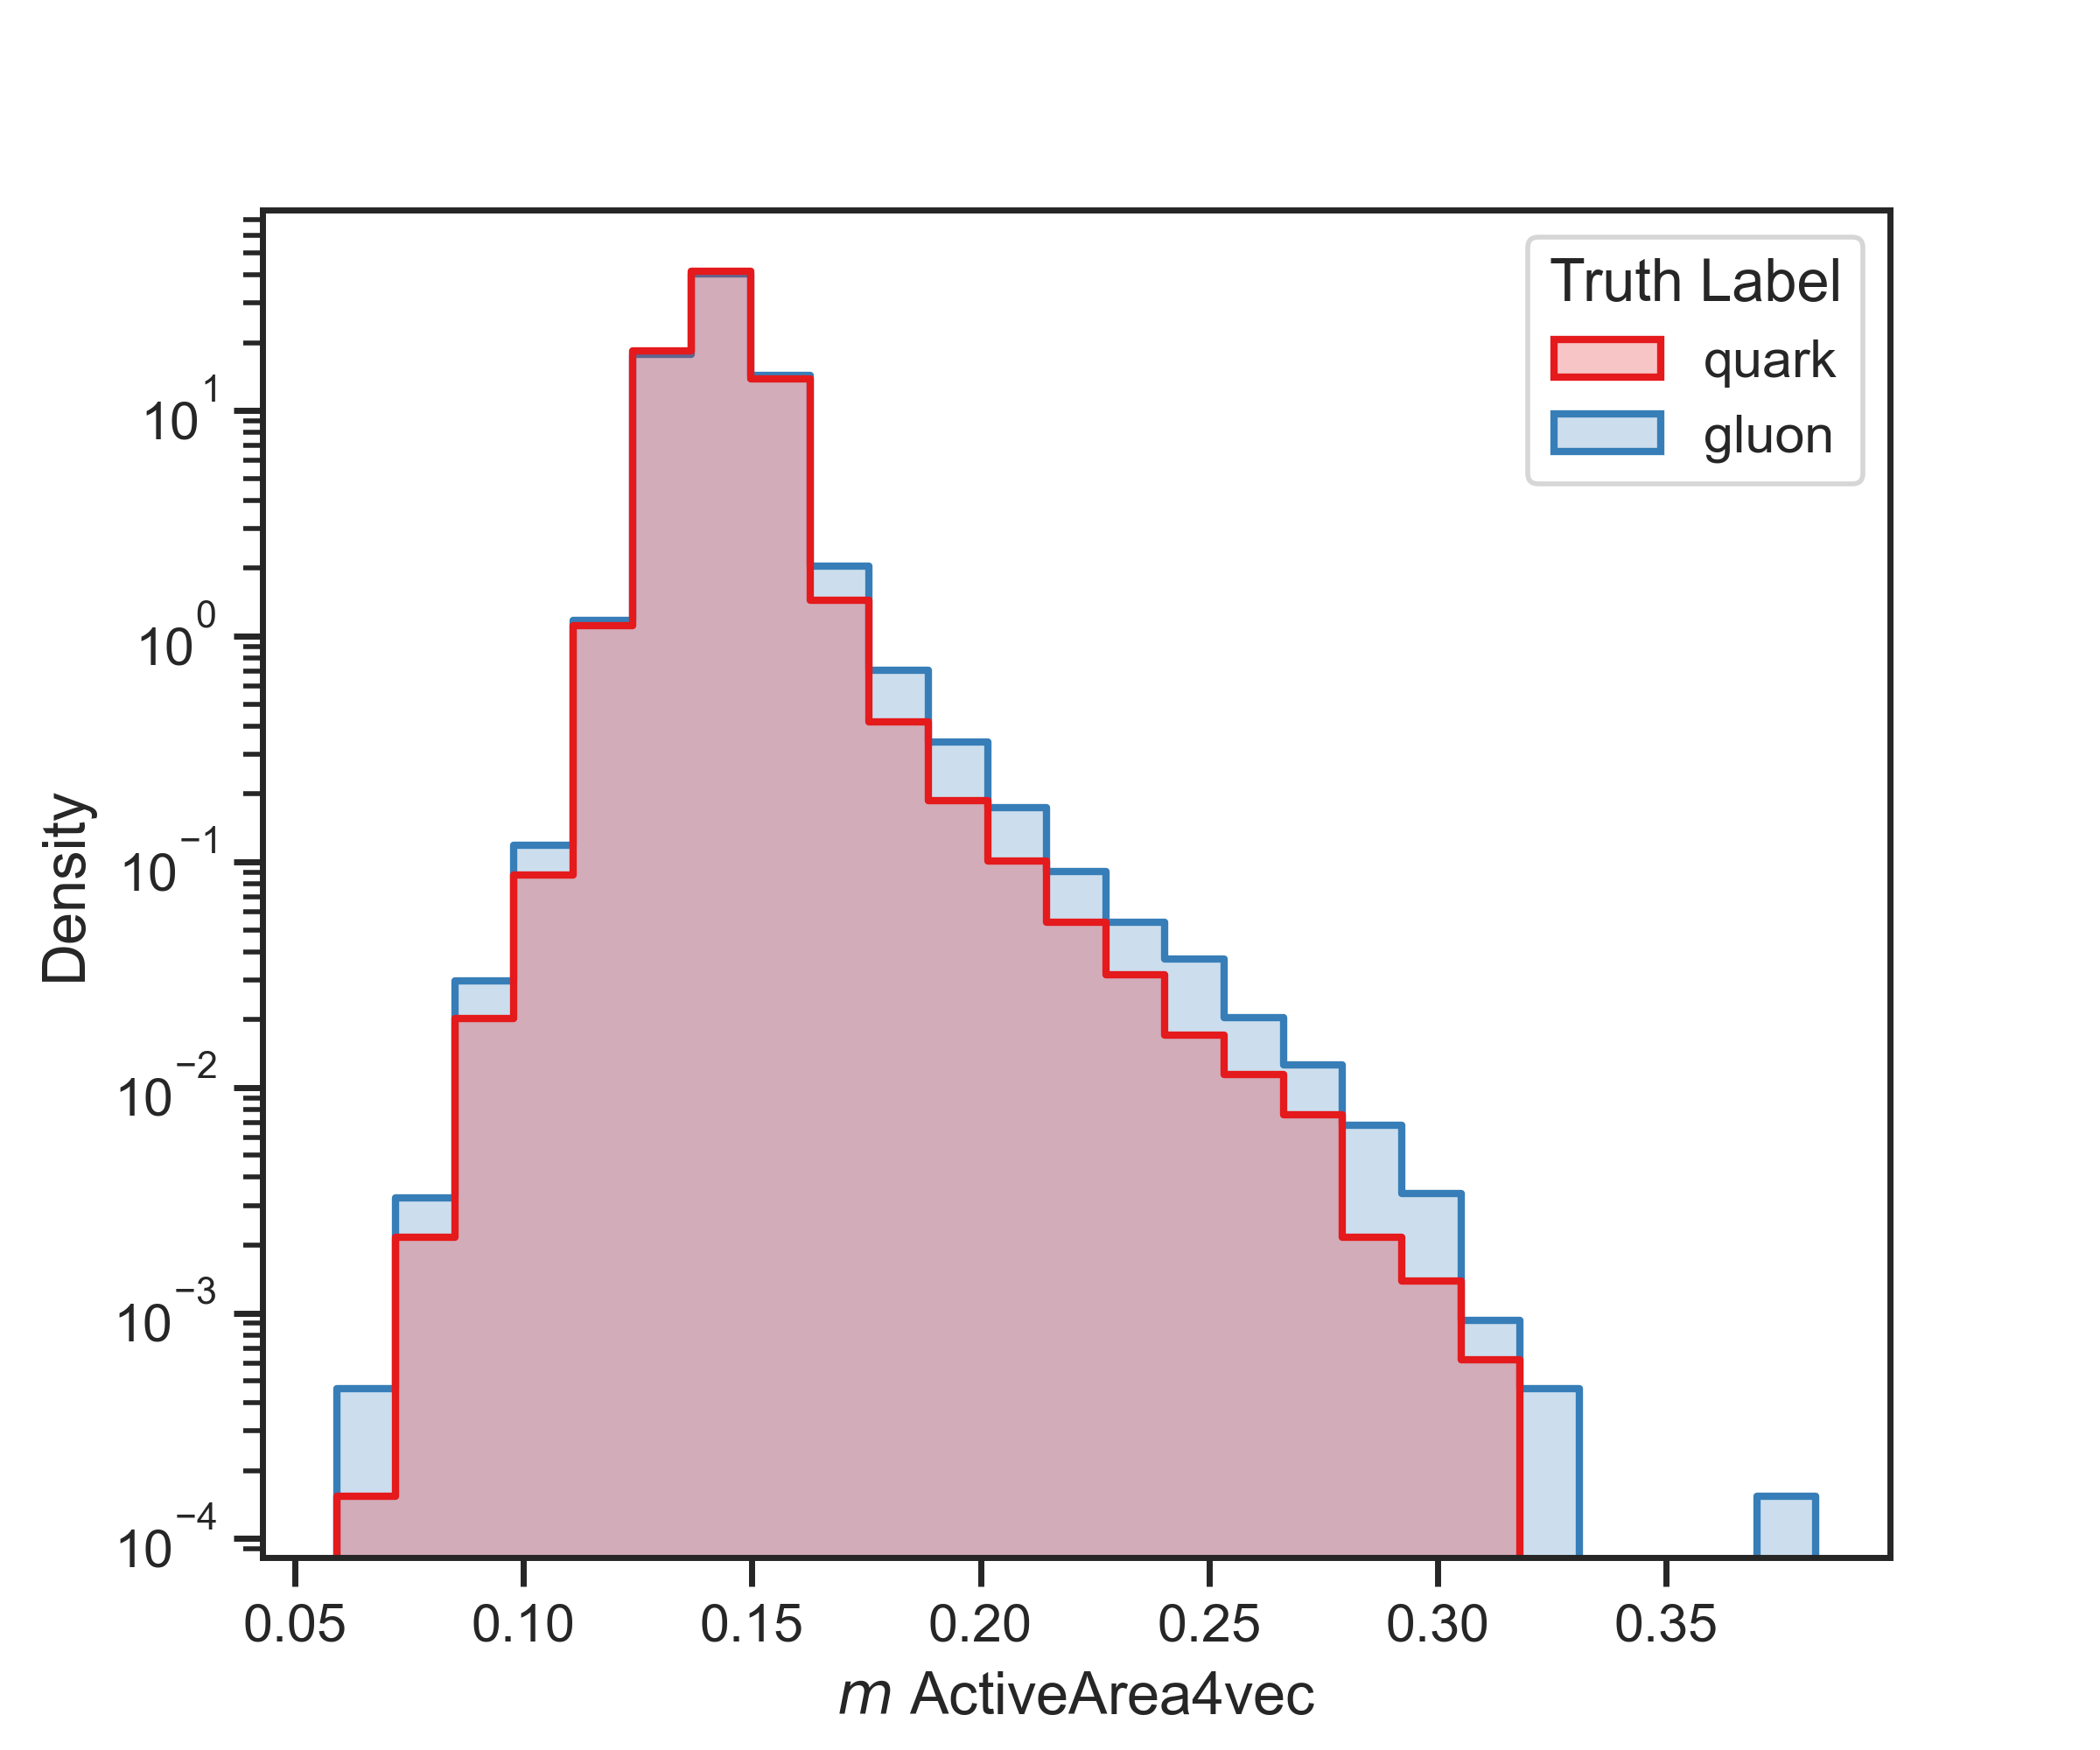
\includegraphics[width=1\textwidth]{src/plots/distributions/highlevel/jets_ActiveArea4vec_m.png}
		\caption{\texttt{jets\_ActiveArea4vec\_m}}
		\label{fig:highlevel_1}
	\end{subfigure}
	\begin{subfigure}[t]{0.48\textwidth}
		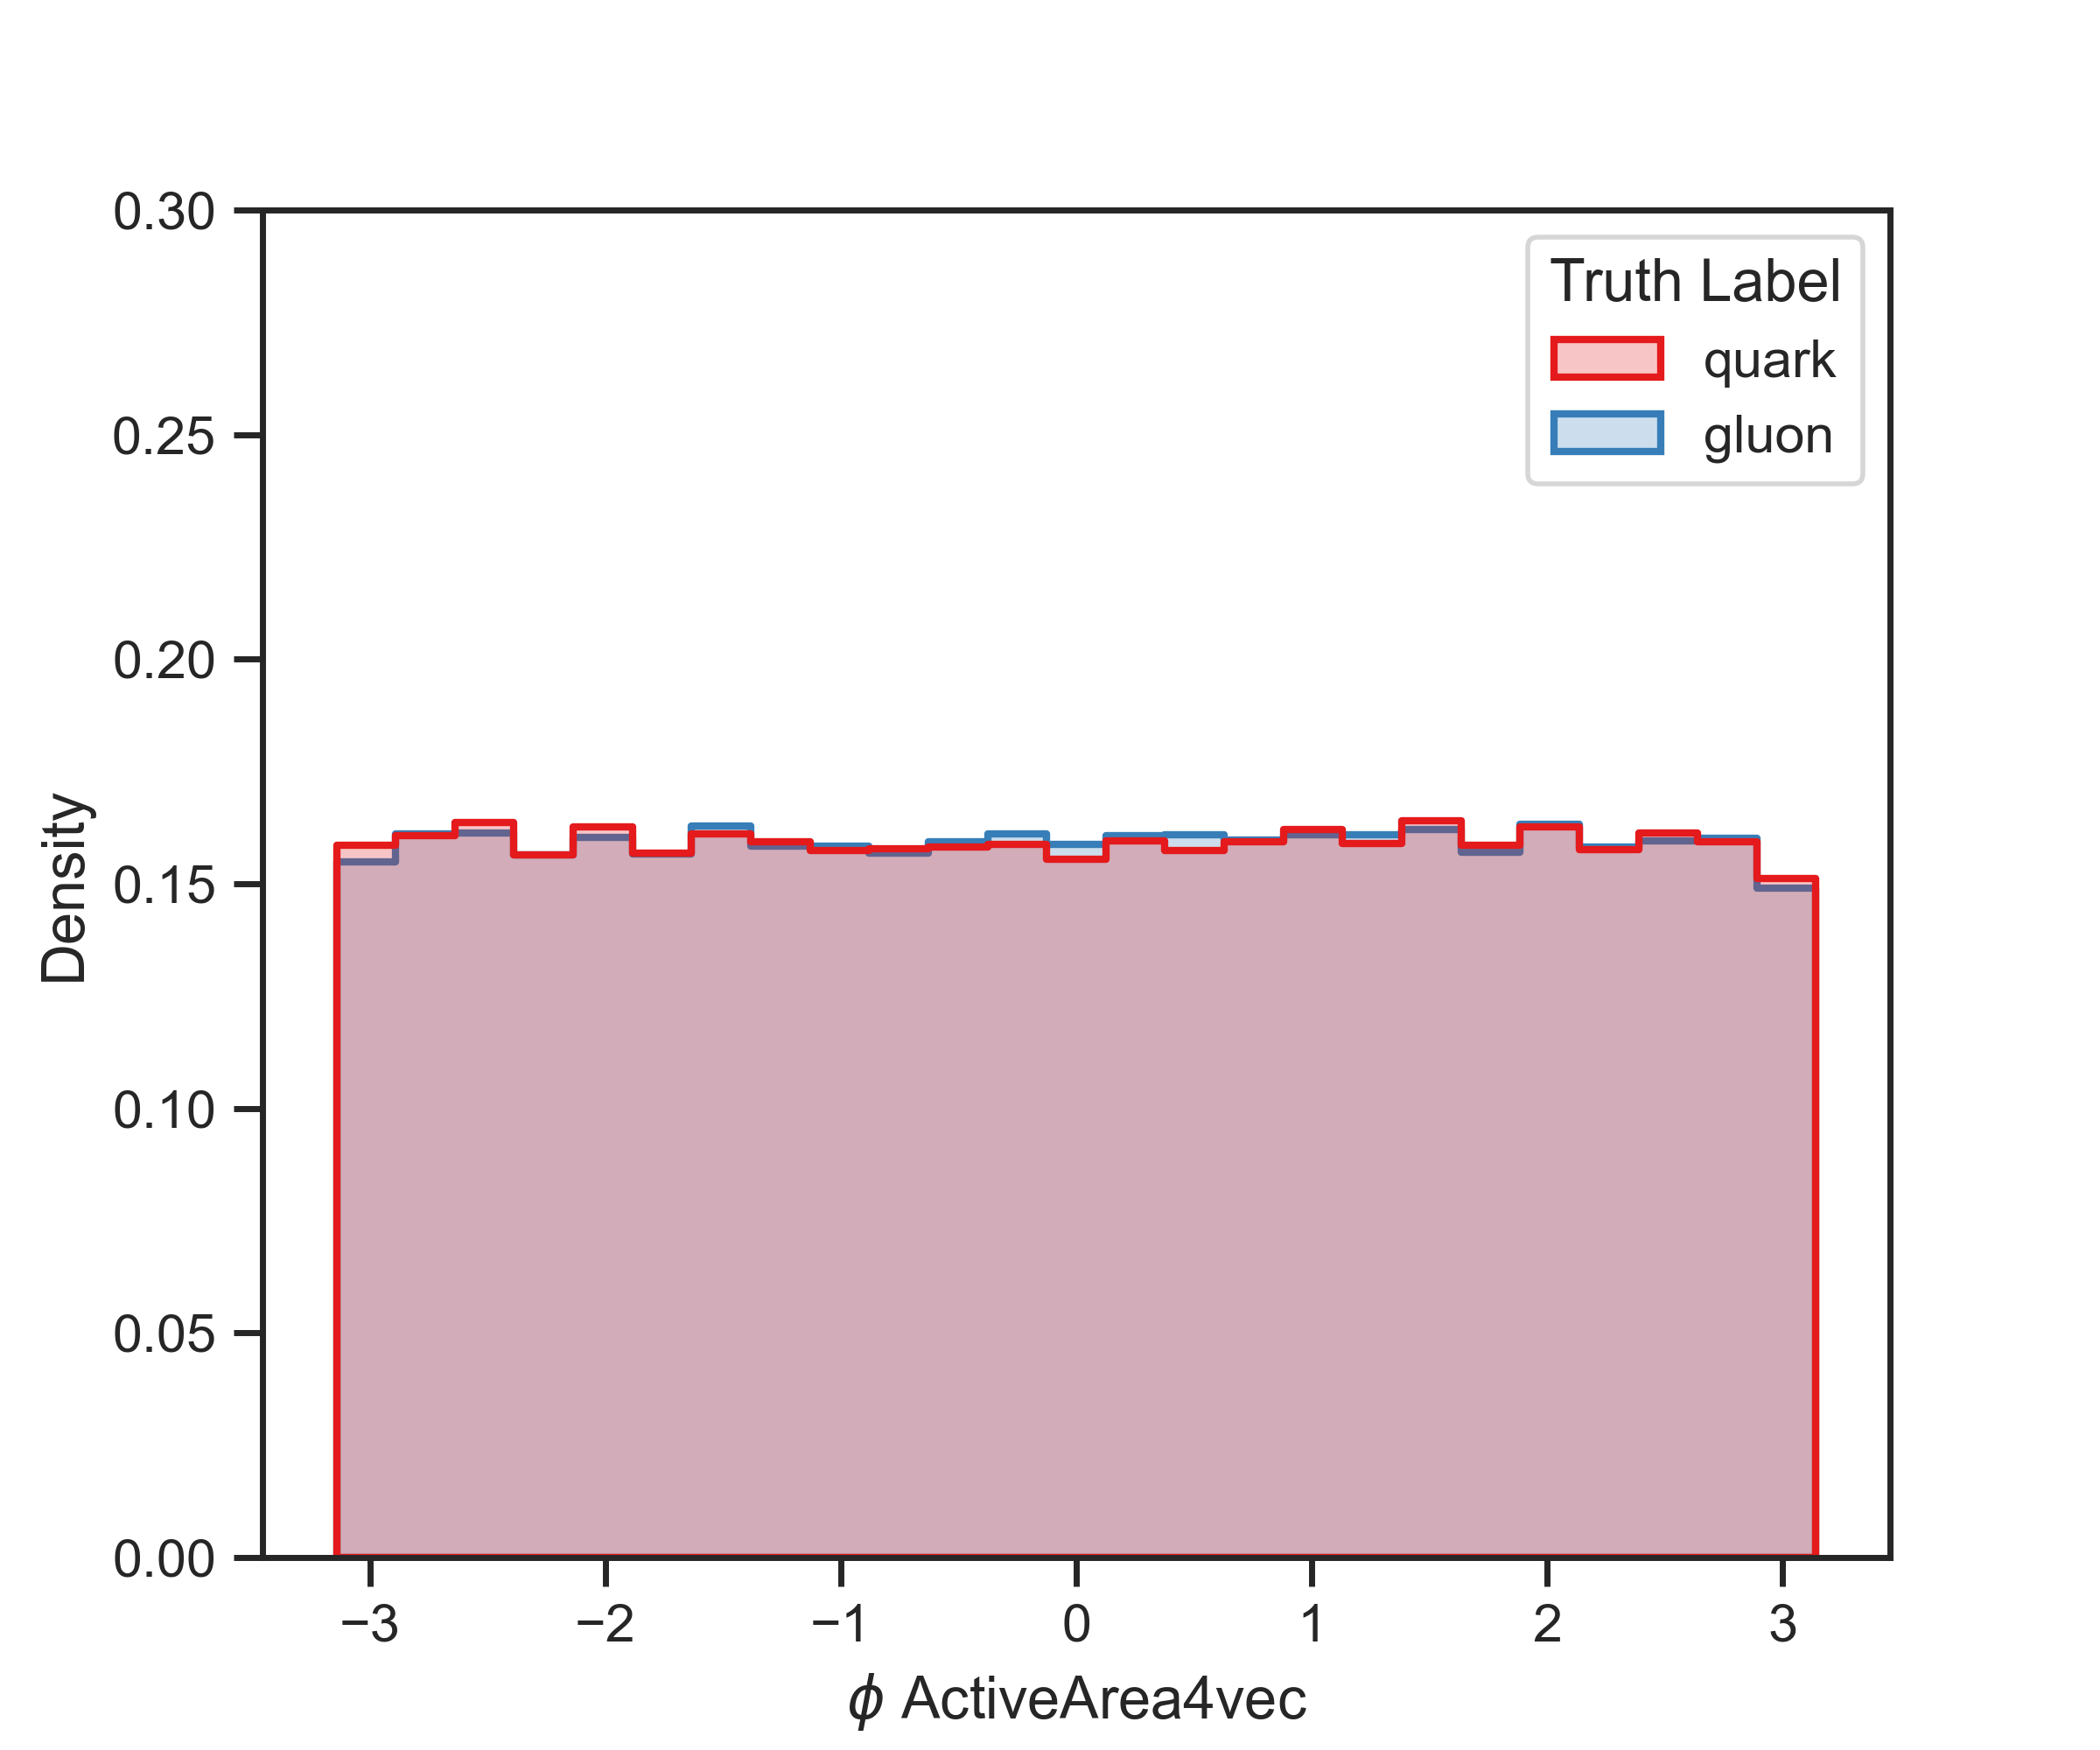
\includegraphics[width=1\textwidth]{src/plots/distributions/highlevel/jets_ActiveArea4vec_phi.png}
		\caption{\texttt{jets\_ActiveArea4vec\_phi}}
		\label{fig:highlevel_2}
	\end{subfigure}
	\begin{subfigure}[t]{0.48\textwidth}
		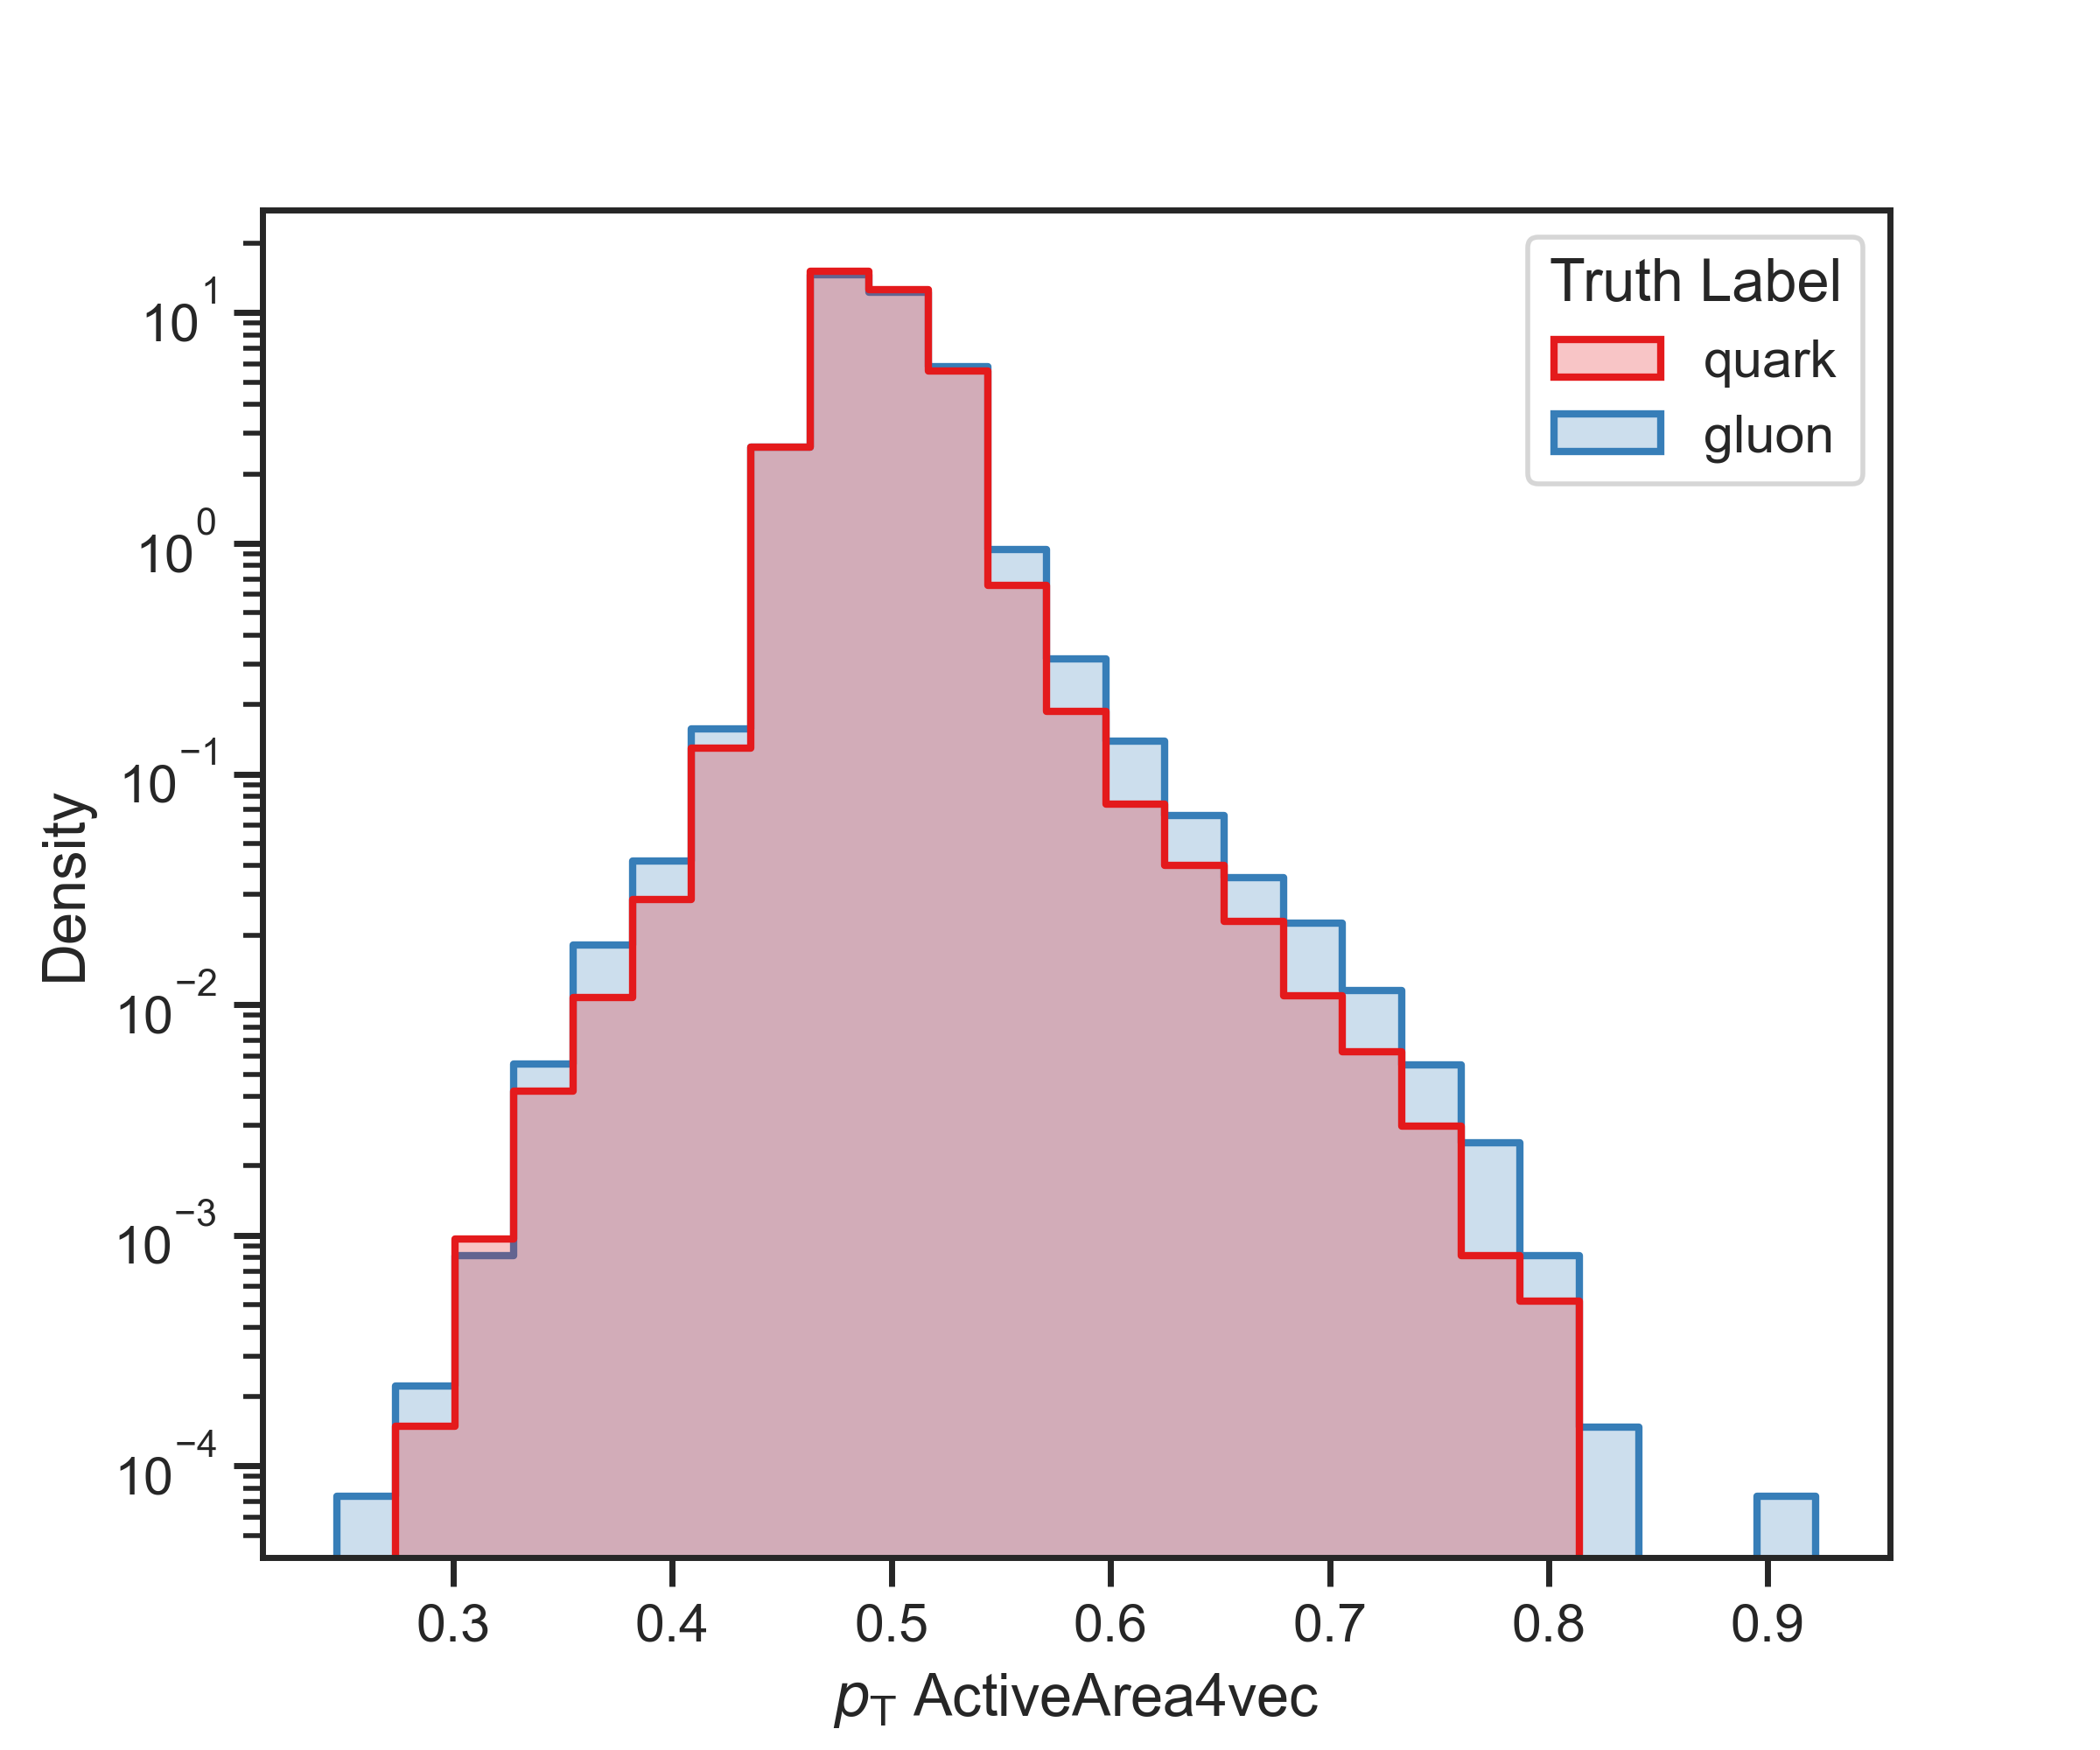
\includegraphics[width=1\textwidth]{src/plots/distributions/highlevel/jets_ActiveArea4vec_pt.png}
		\caption{\texttt{jets\_ActiveArea4vec\_pt}}
		\label{fig:highlevel_3}
	\end{subfigure}
	\begin{subfigure}[t]{0.48\textwidth}
		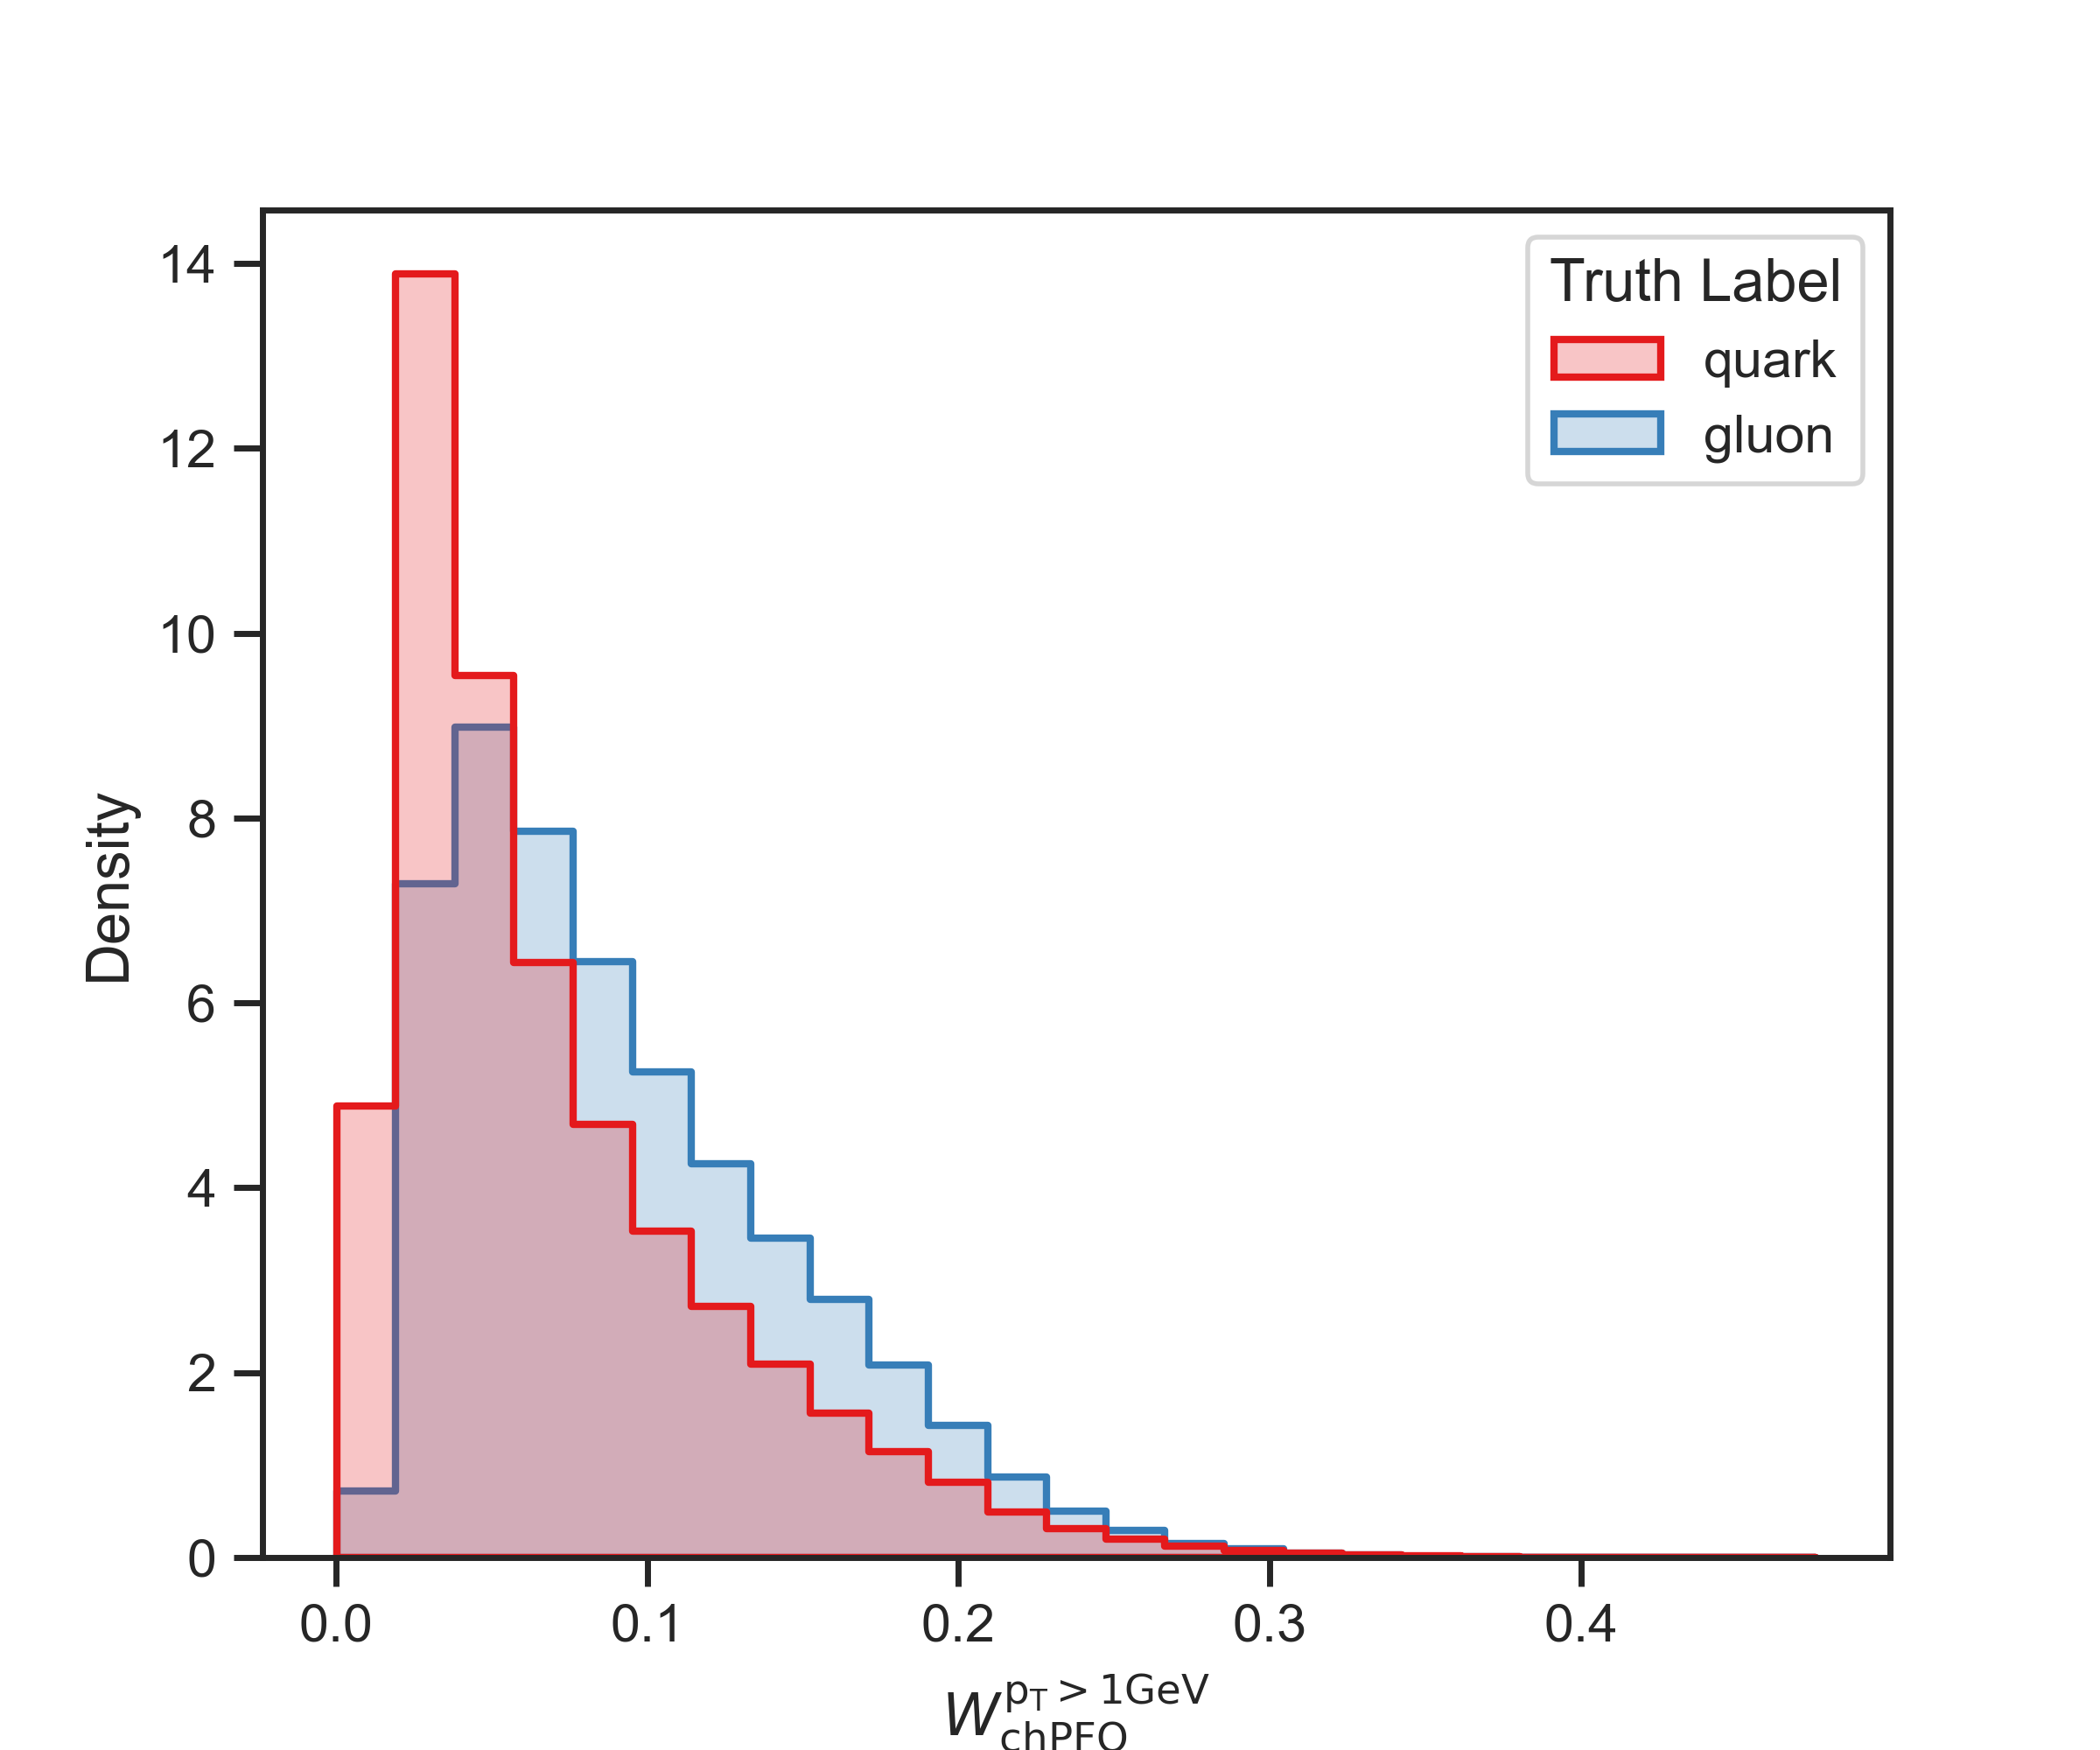
\includegraphics[width=1\textwidth]{src/plots/distributions/highlevel/jets_ChargedPFOWidthPt1000[0].png}
		\caption{\texttt{jets\_ChargedPFOWidthPt1000[0]}}
		\label{fig:highlevel_4}
	\end{subfigure}
	\begin{subfigure}[t]{0.48\textwidth}
		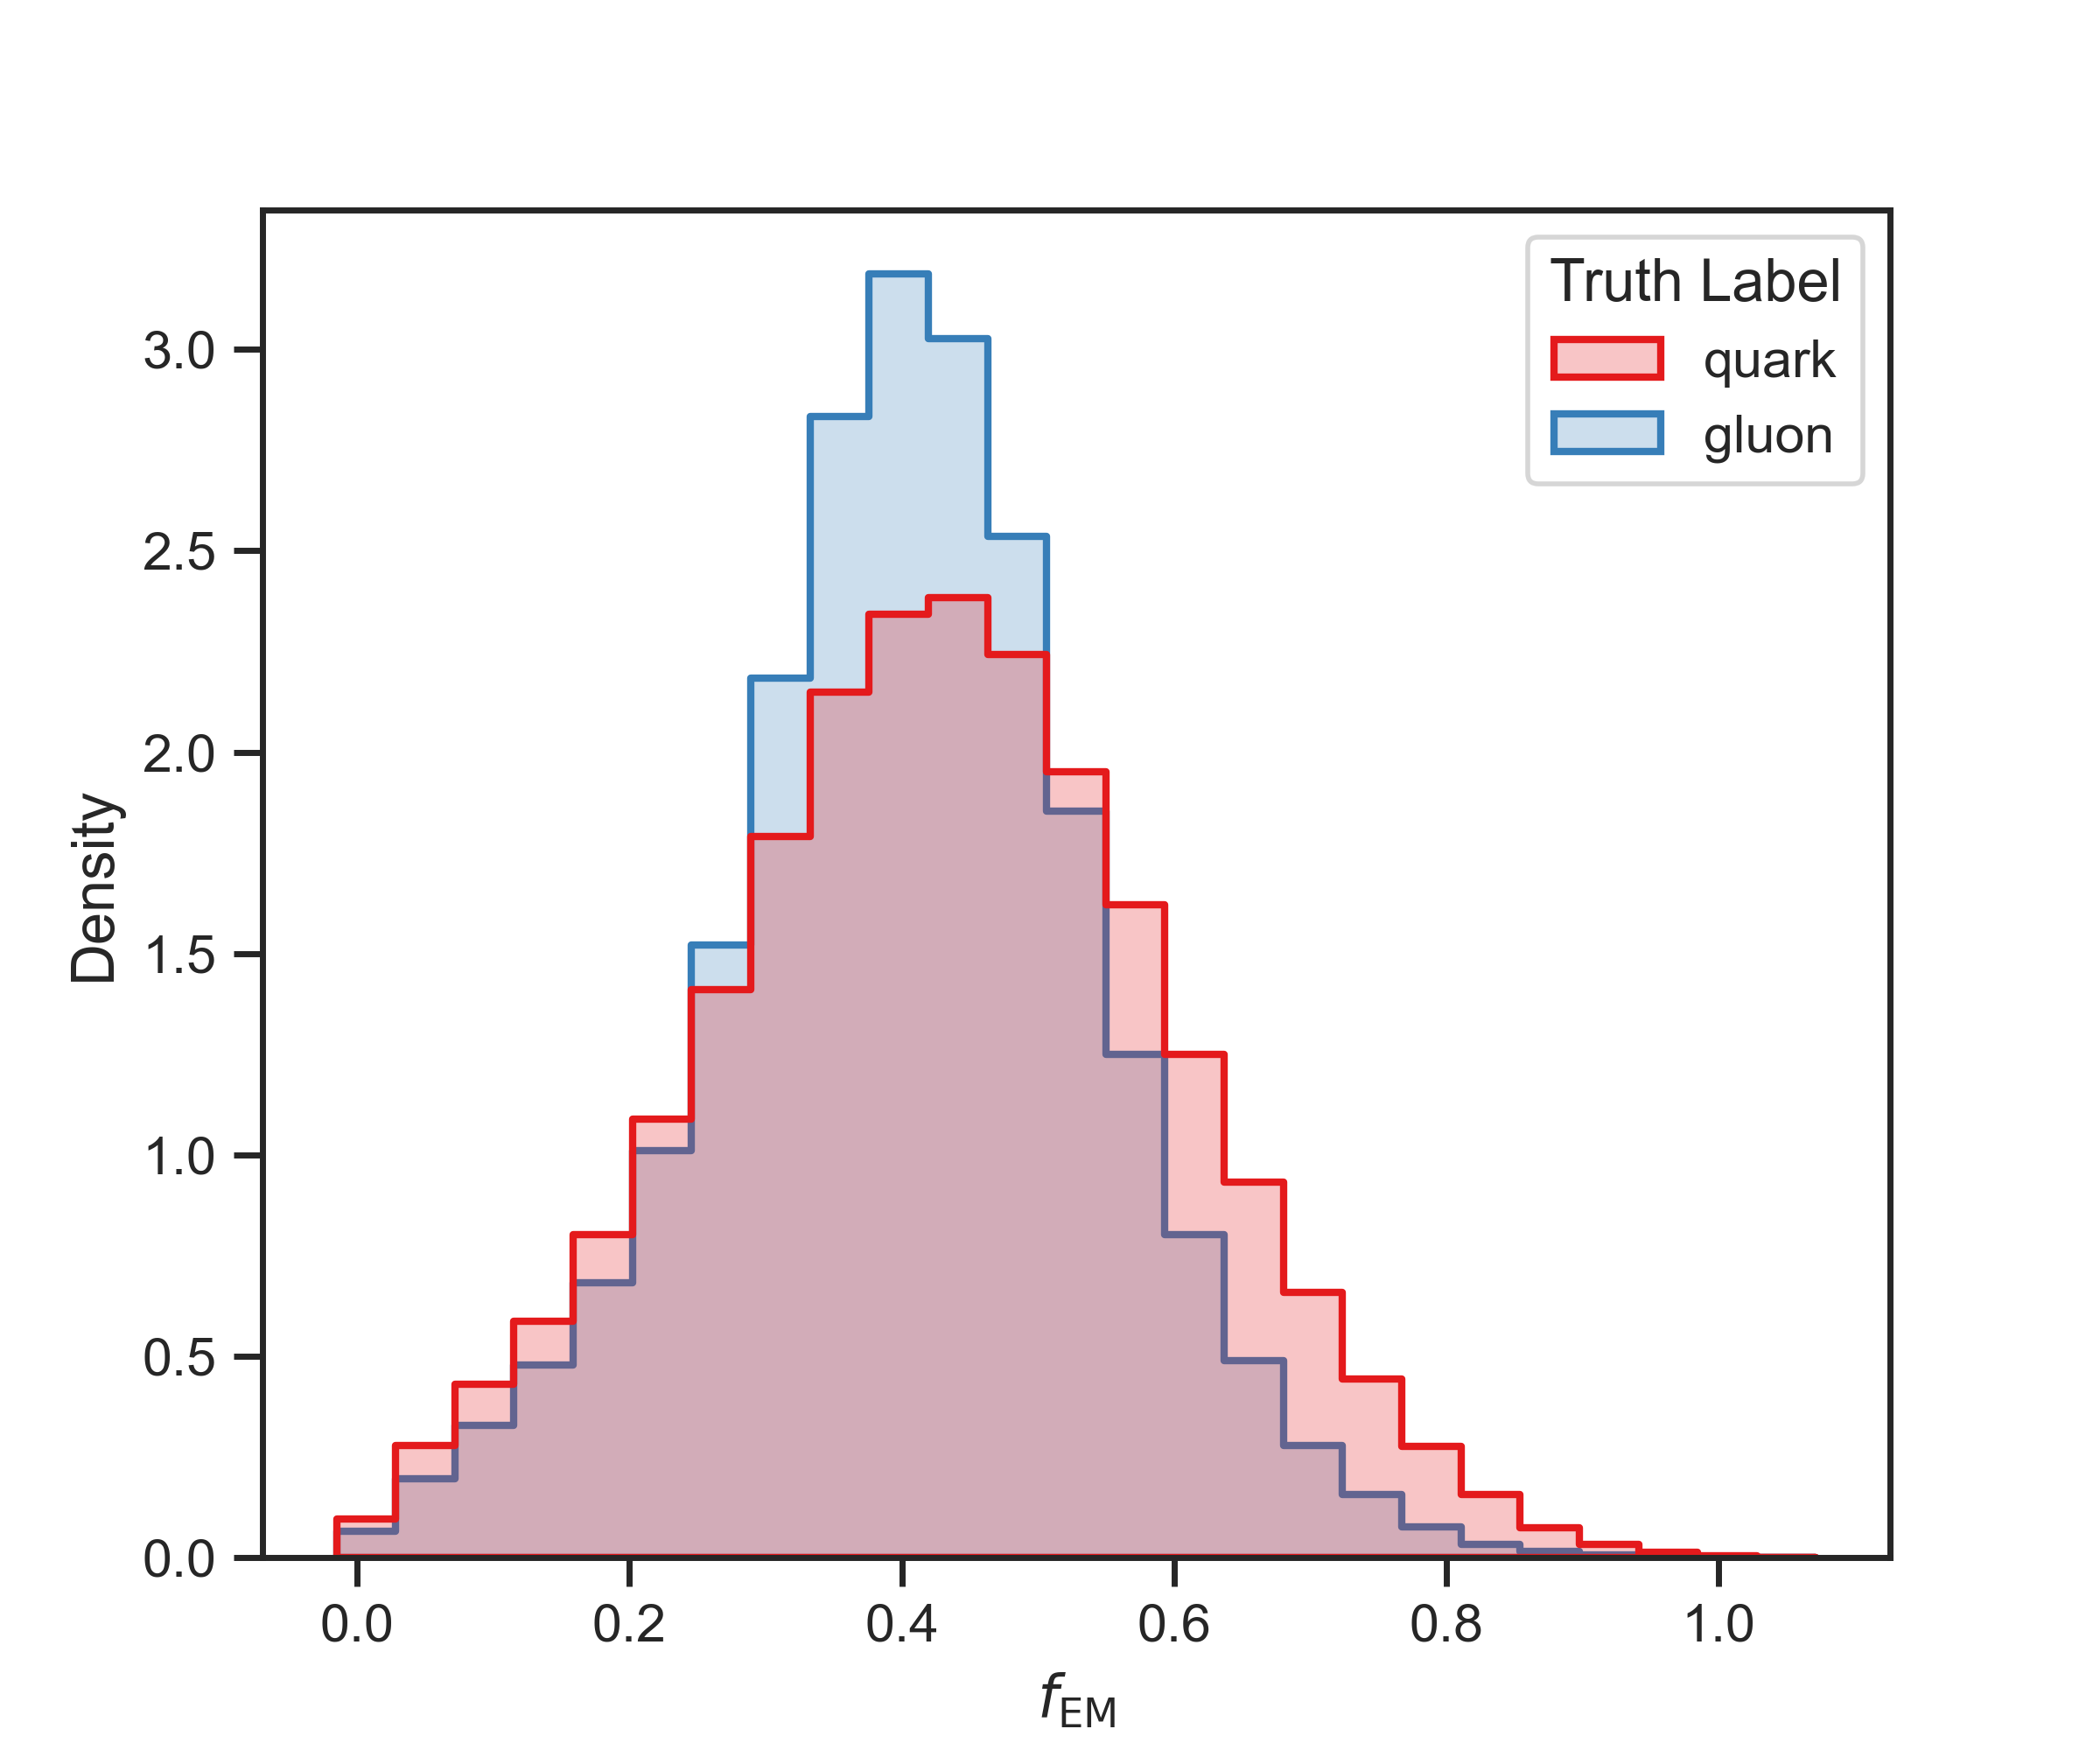
\includegraphics[width=1\textwidth]{src/plots/distributions/highlevel/jets_EMFrac.png}
		\caption{\texttt{jets\_EMFrac}}
		\label{fig:highlevel_5}
	\end{subfigure}
\caption{High-level Jet Variables, part 1}
\label{fig:highlevel_0-5}
\end{figure}

\begin{figure}[!htb]
	\centering
	\begin{subfigure}[t]{0.48\textwidth}
		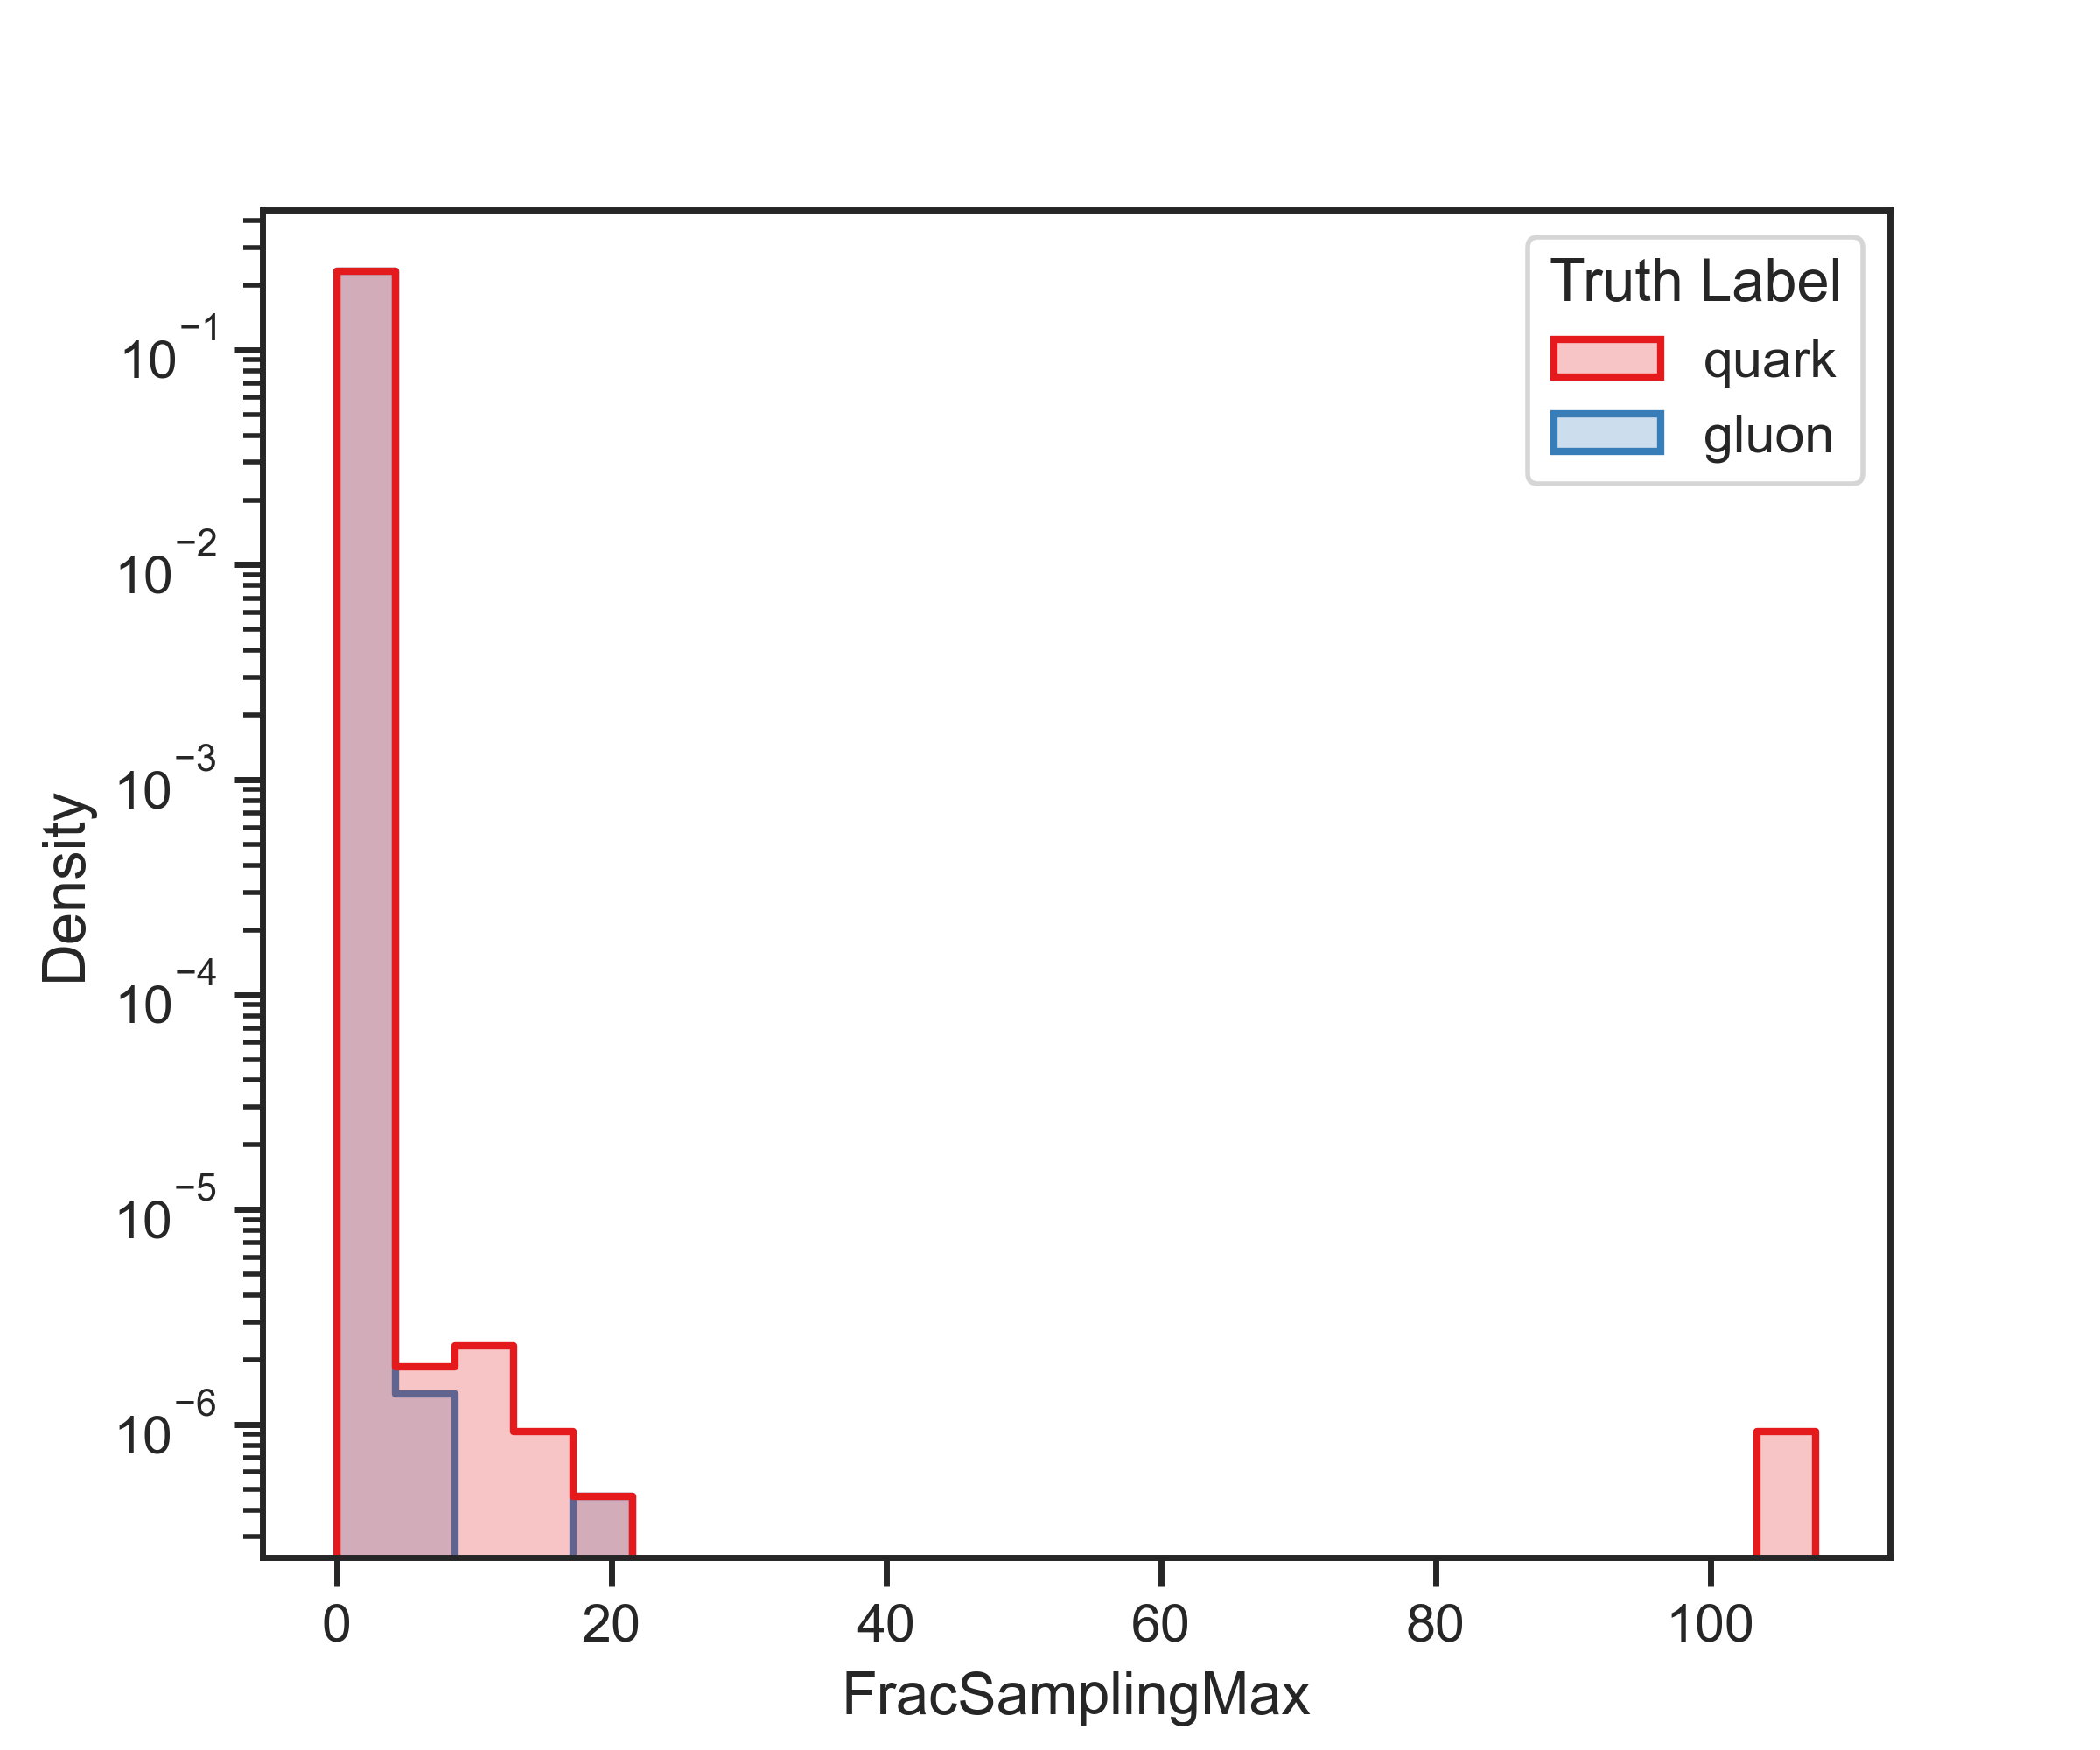
\includegraphics[width=1\textwidth]{src/plots/distributions/highlevel/jets_FracSamplingMax.png}
		\caption{\texttt{jets\_FracSamplingMax}}
		\label{fig:highlevel_6}
	\end{subfigure}
	\begin{subfigure}[t]{0.48\textwidth}
		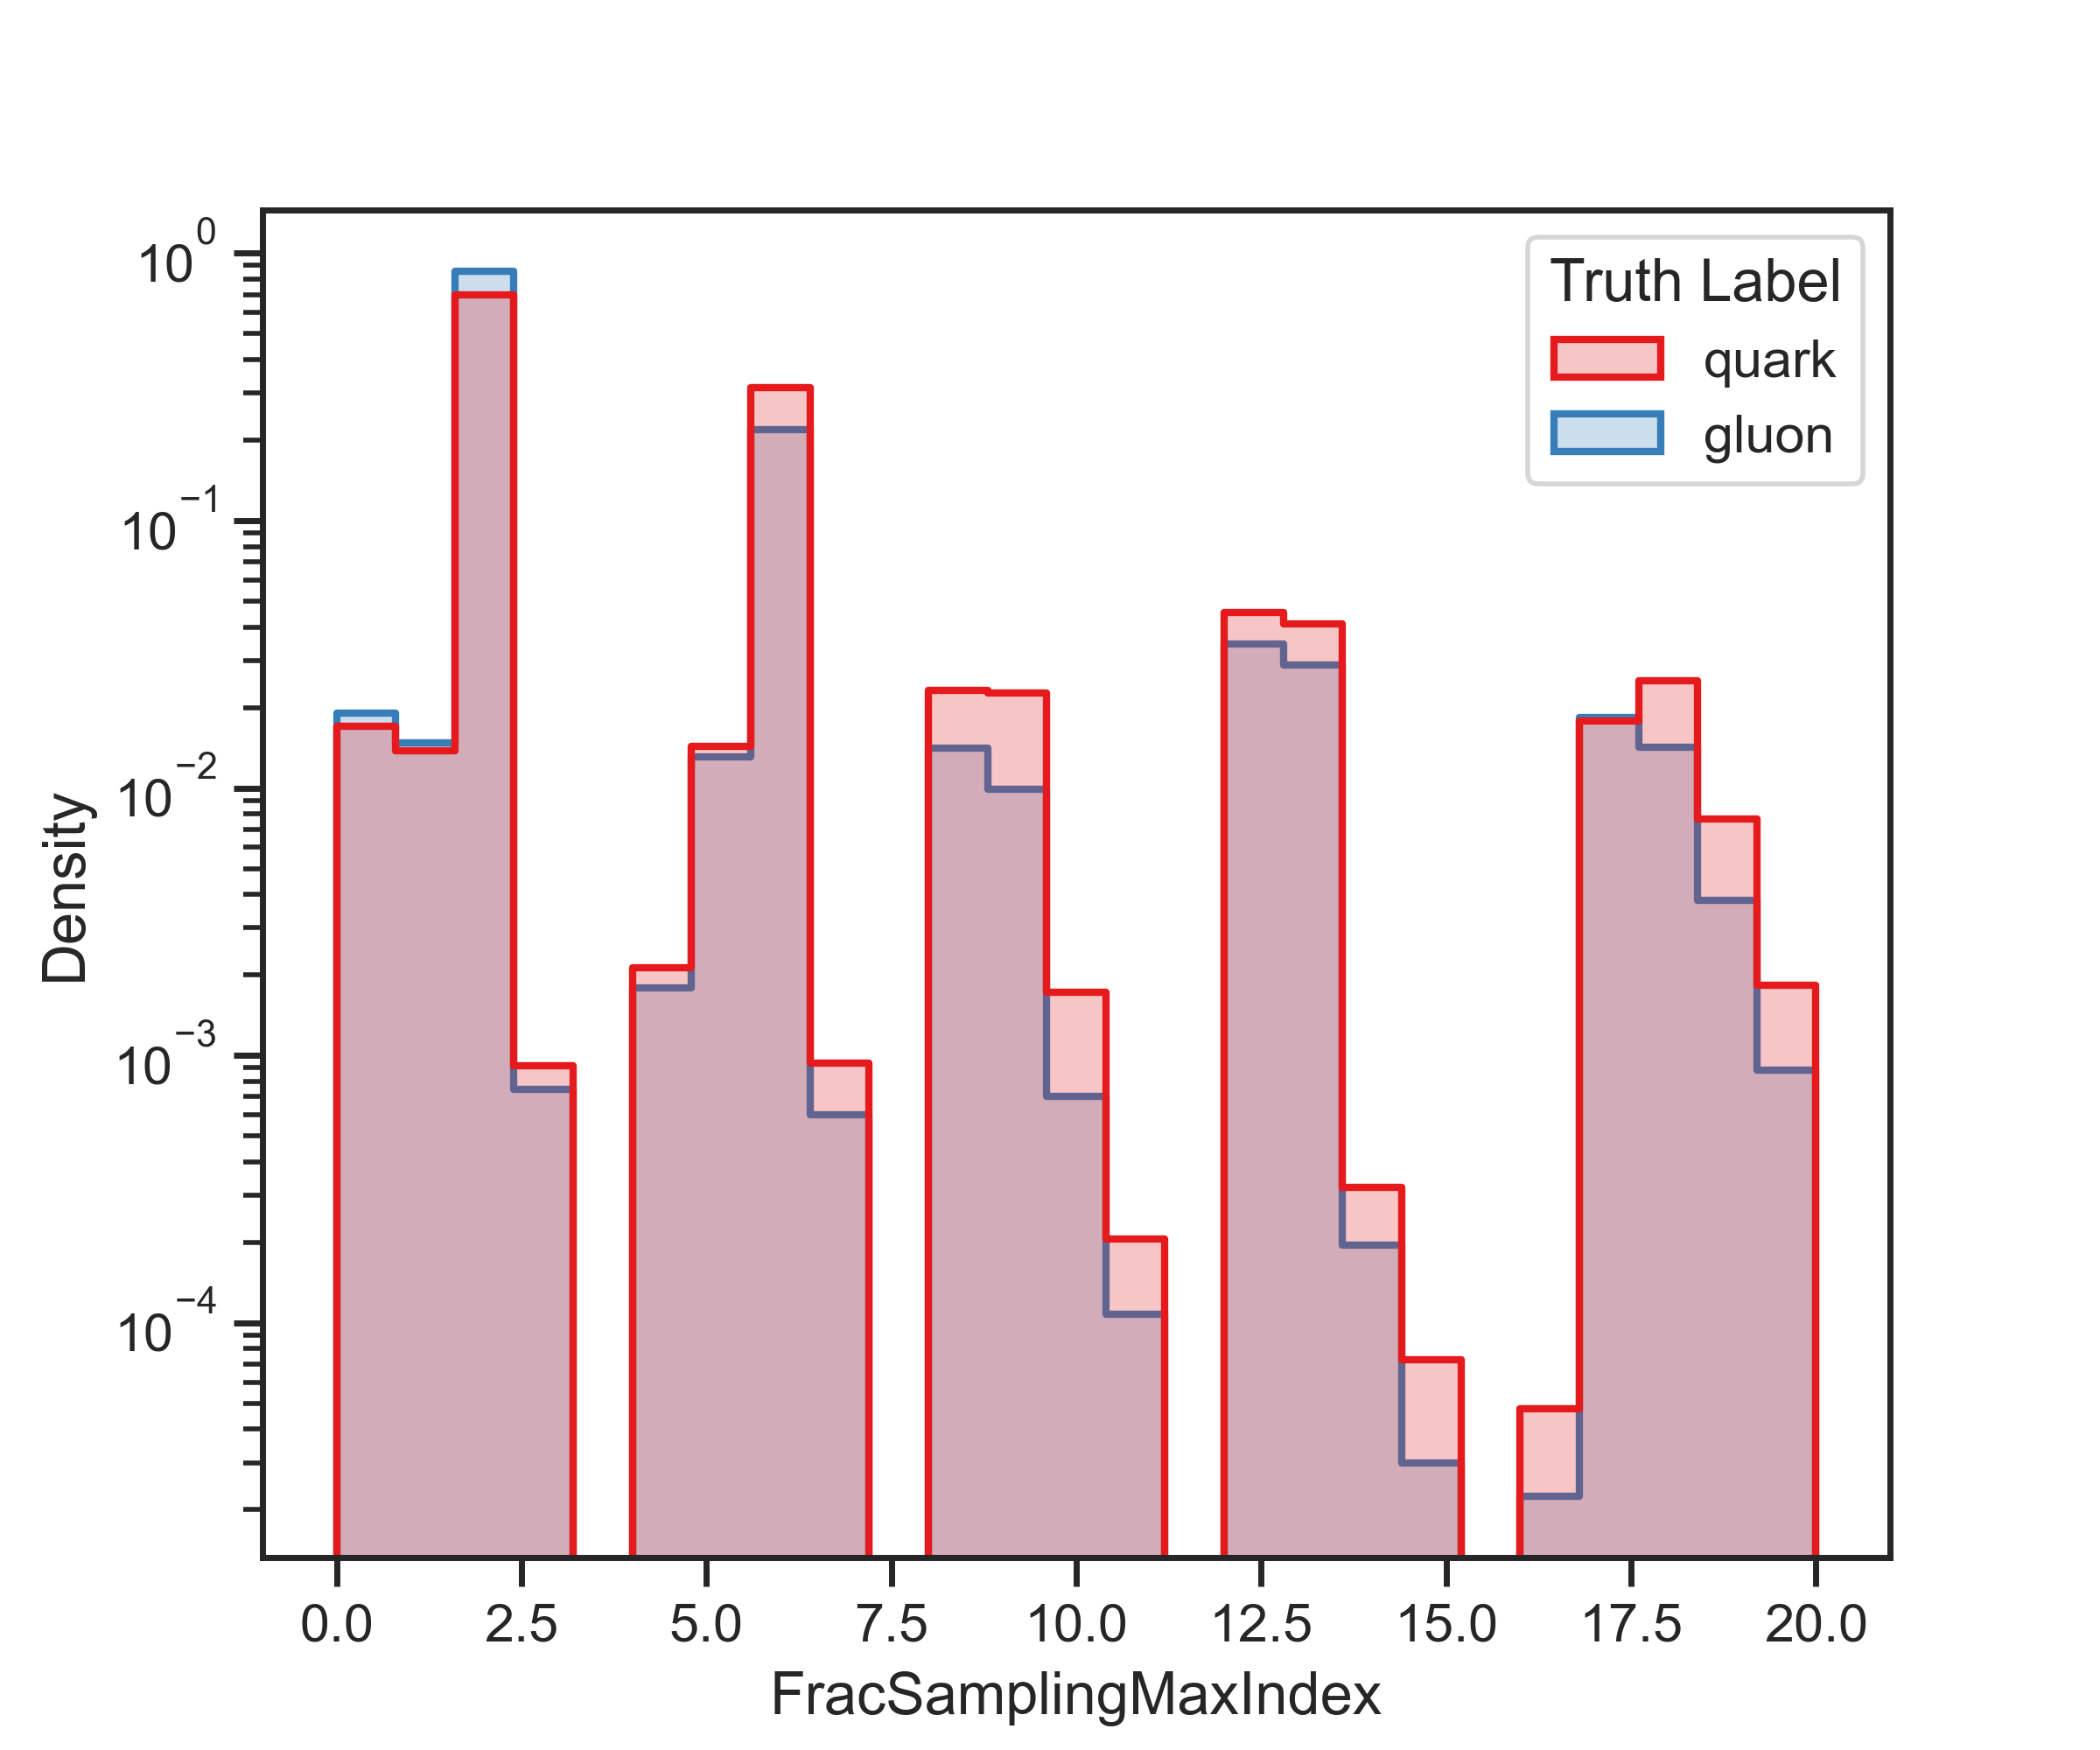
\includegraphics[width=1\textwidth]{src/plots/distributions/highlevel/jets_FracSamplingMaxIndex.png}
		\caption{\texttt{jets\_FracSamplingMaxIndex}}
		\label{fig:highlevel_7}
	\end{subfigure}
	\begin{subfigure}[t]{0.48\textwidth}
		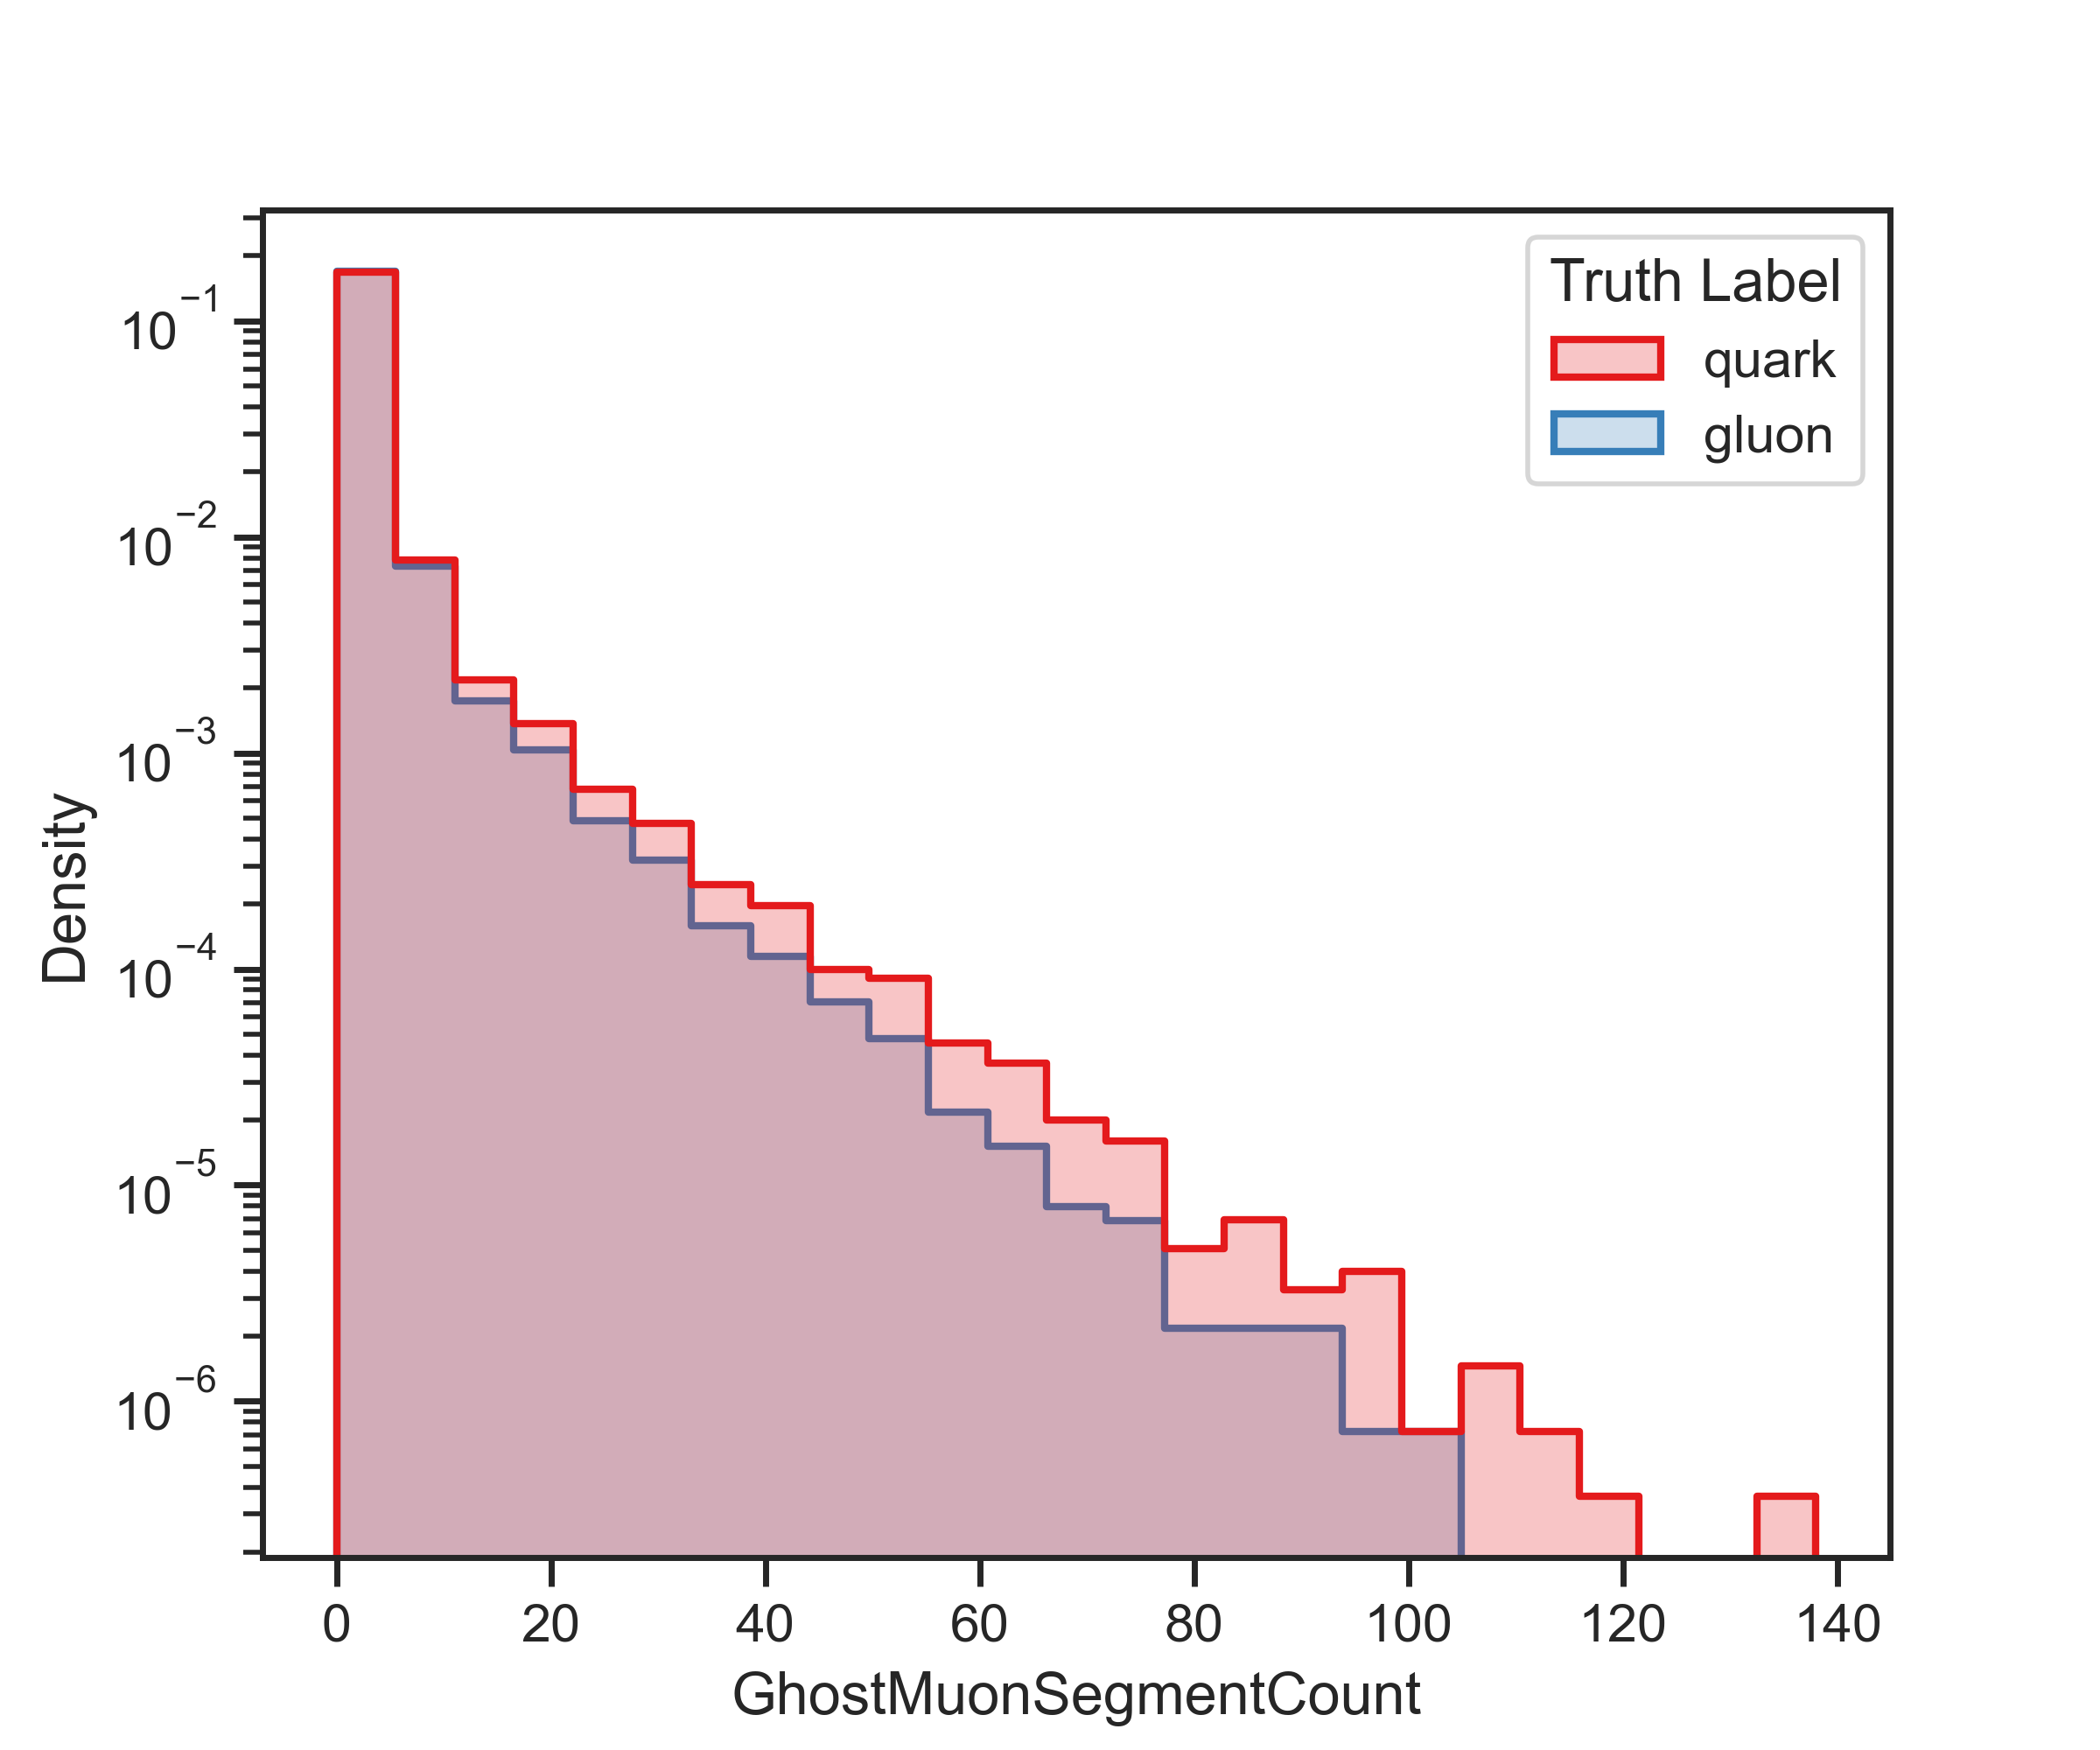
\includegraphics[width=1\textwidth]{src/plots/distributions/highlevel/jets_GhostMuonSegmentCount.png}
		\caption{\texttt{jets\_GhostMuonSegmentCount}}
		\label{fig:highlevel_8}
	\end{subfigure}
	\begin{subfigure}[t]{0.48\textwidth}
		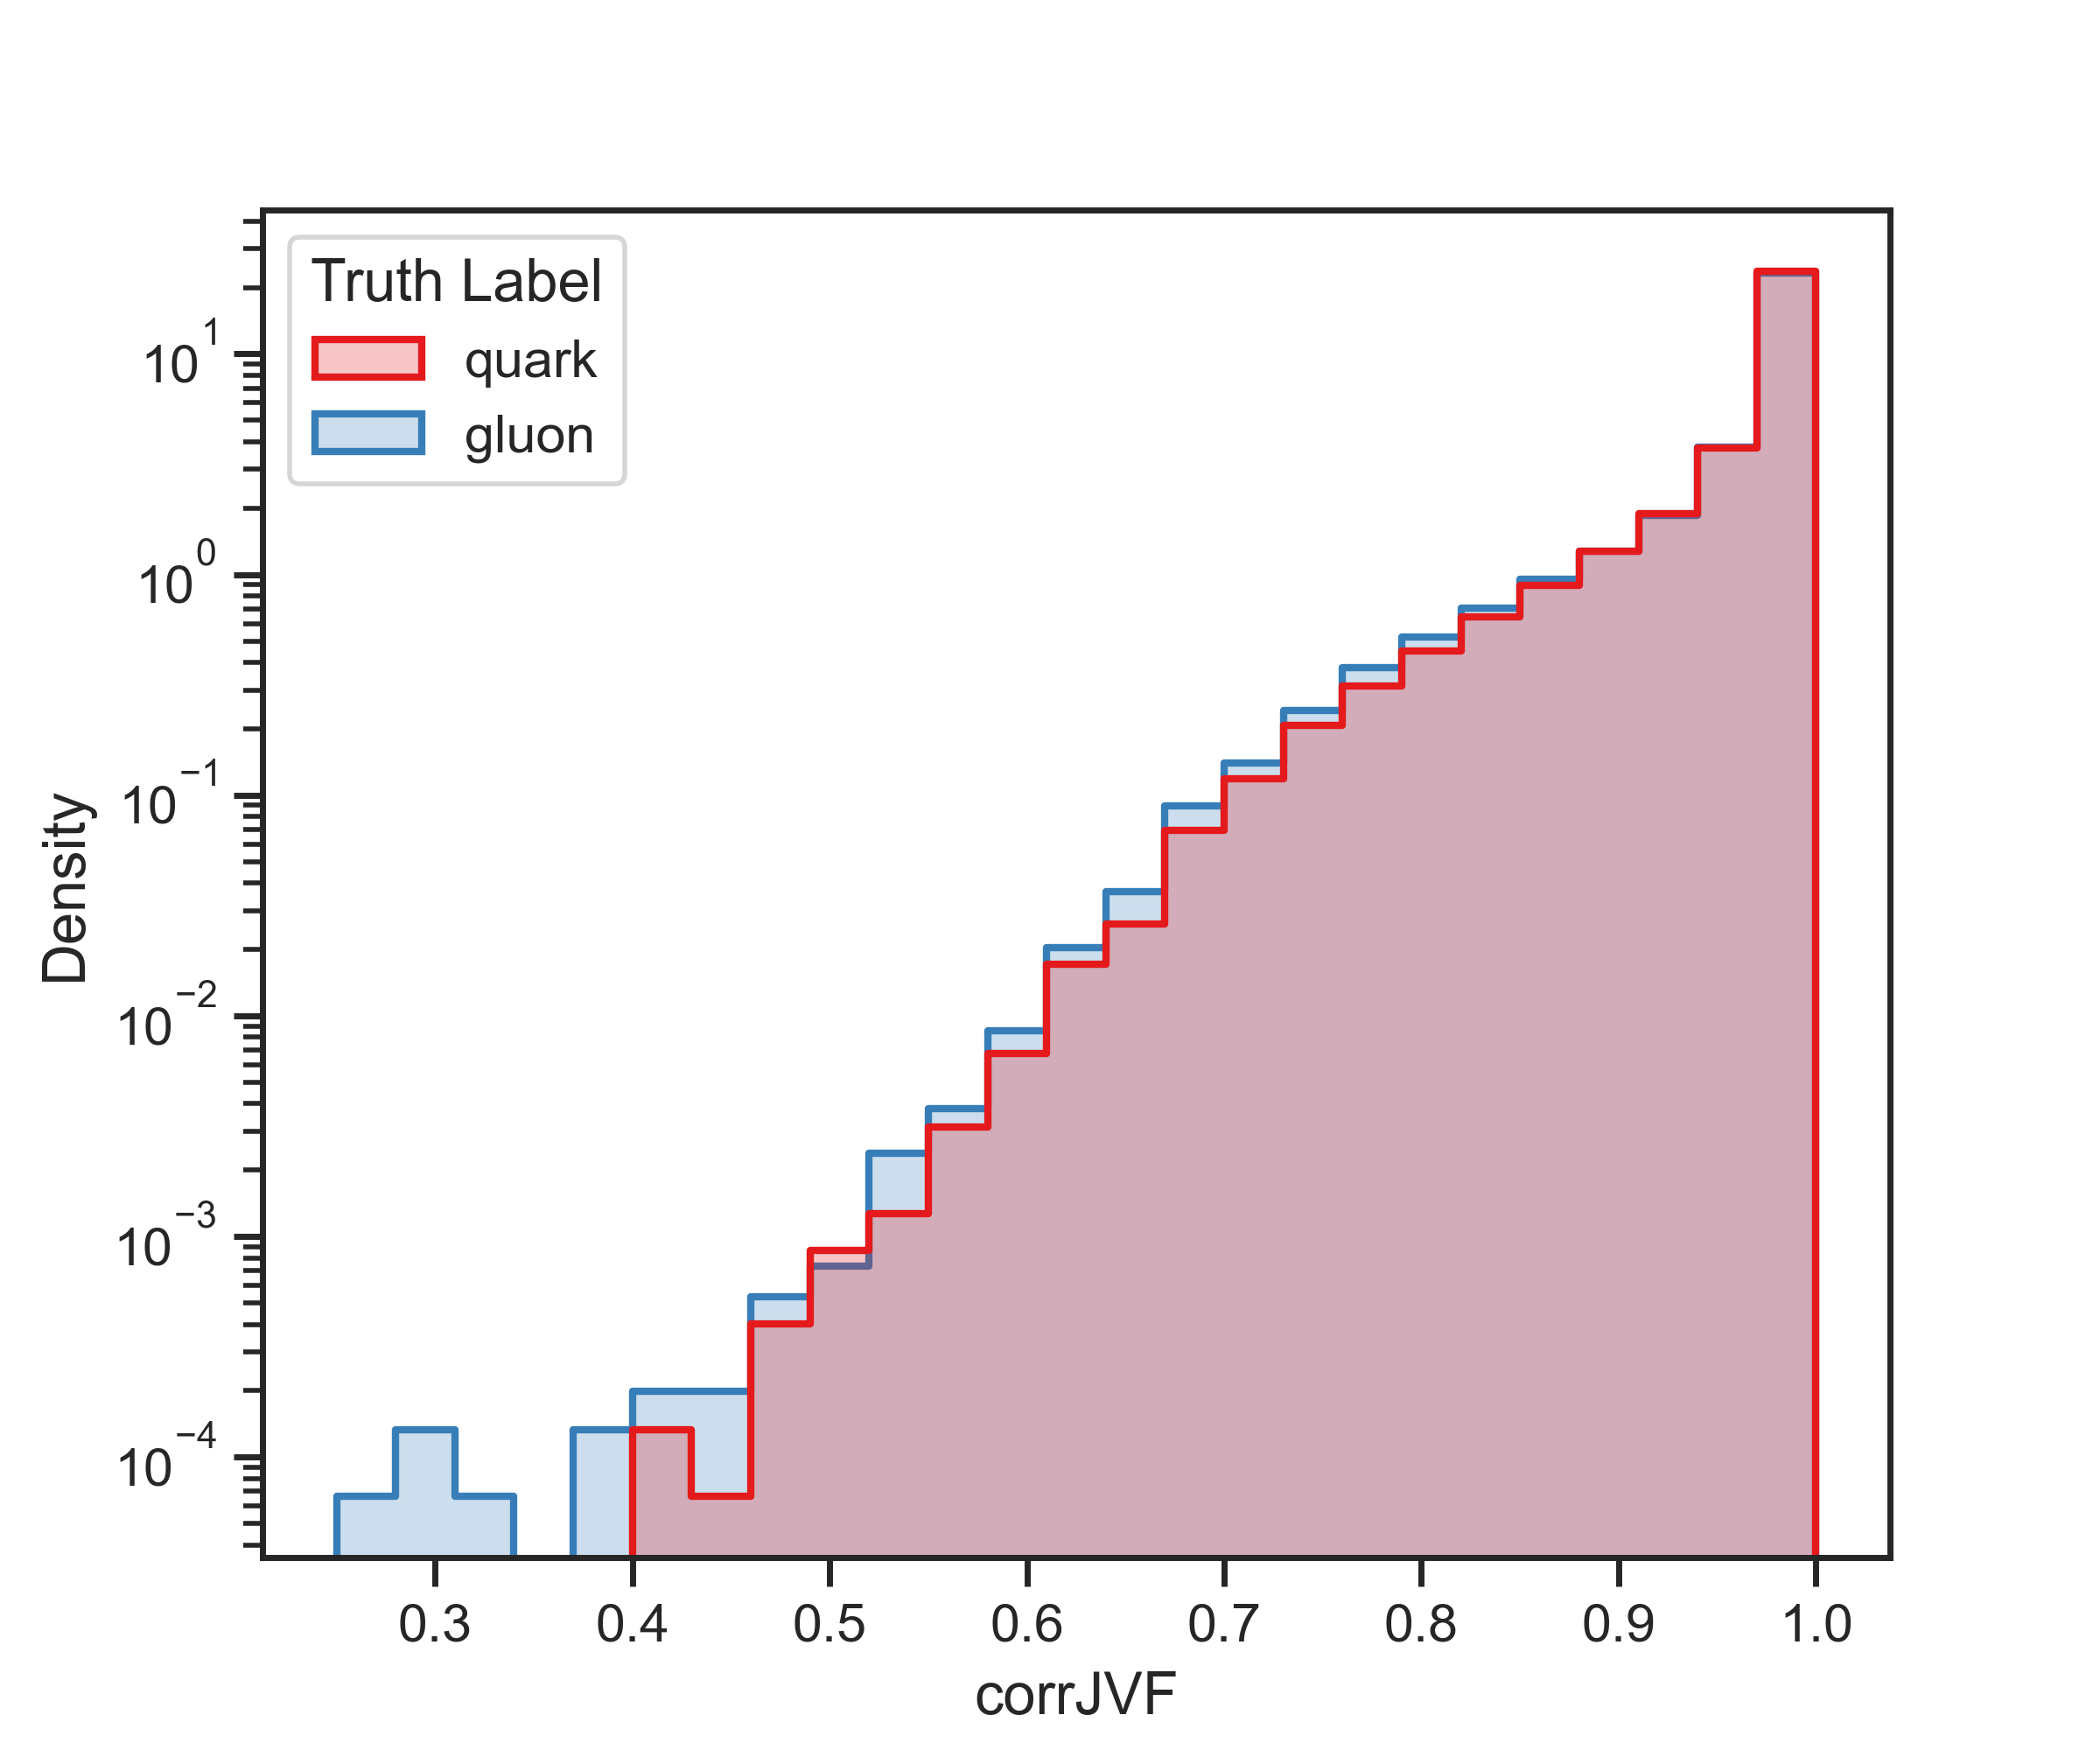
\includegraphics[width=1\textwidth]{src/plots/distributions/highlevel/jets_JVFCorr.png}
		\caption{\texttt{jets\_JVFCorr}}
		\label{fig:highlevel_9}
	\end{subfigure}
	\begin{subfigure}[t]{0.48\textwidth}
		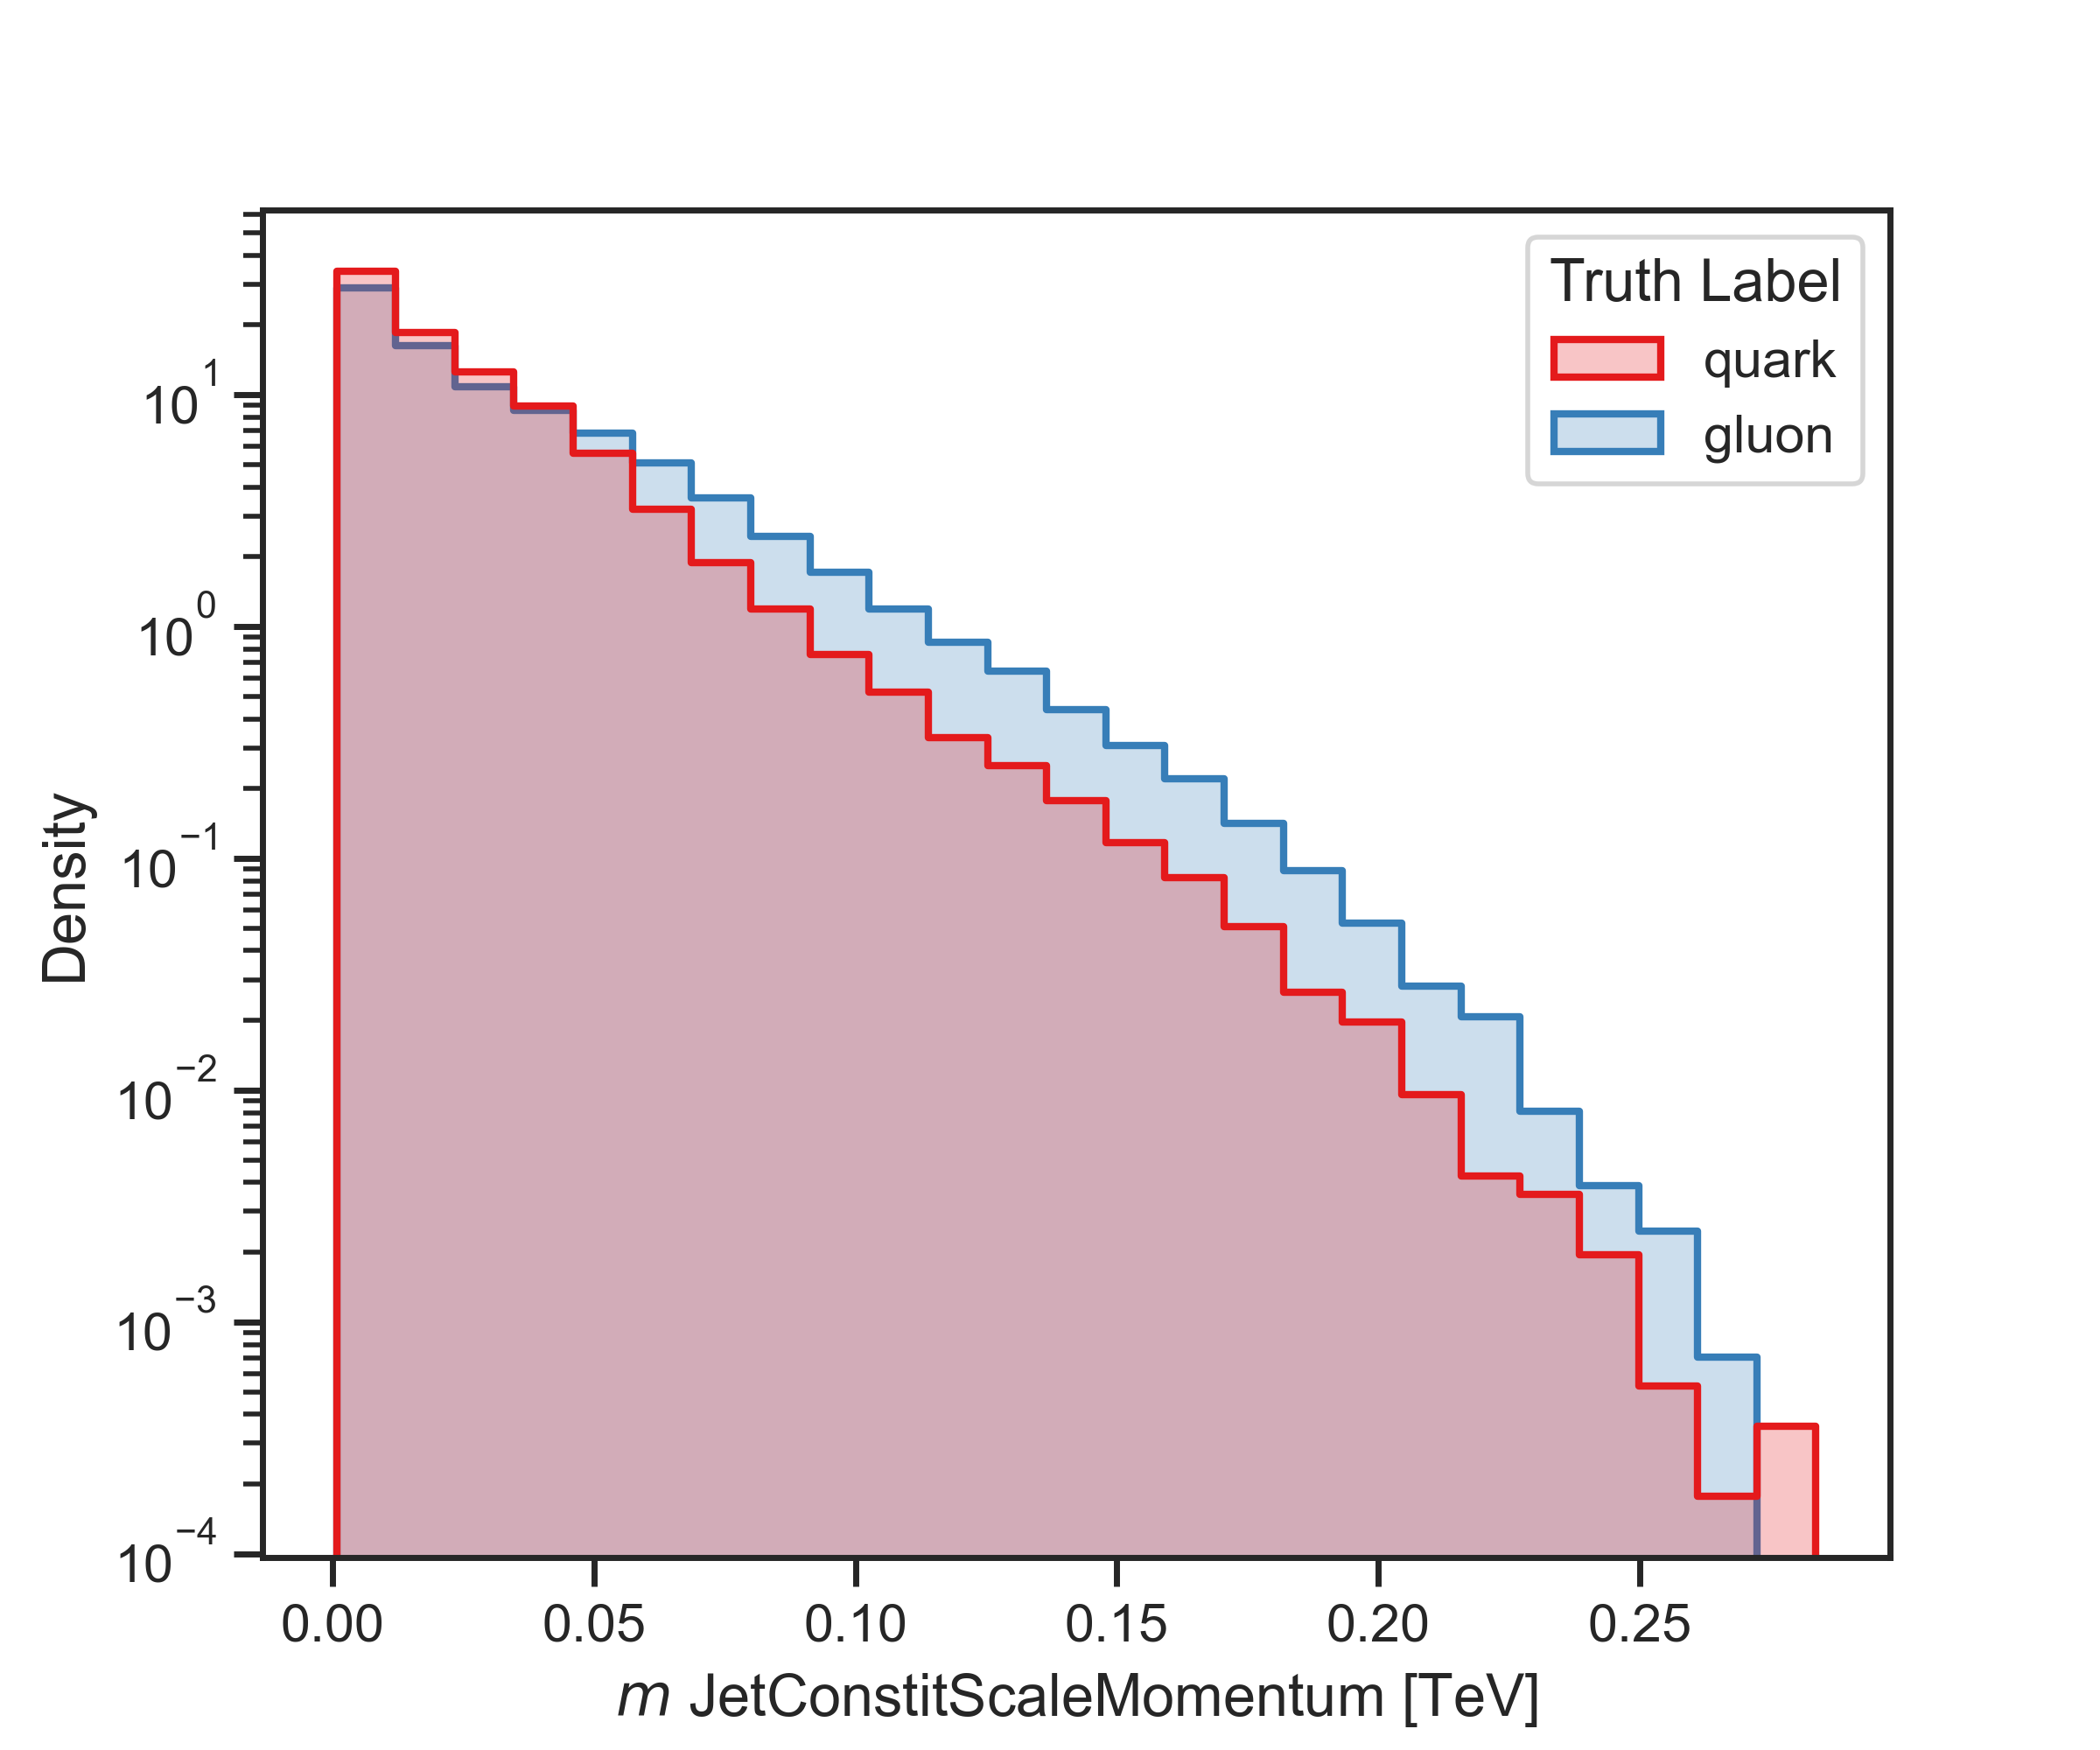
\includegraphics[width=1\textwidth]{src/plots/distributions/highlevel/jets_JetConstitScaleMomentum_m.png}
		\caption{\texttt{jets\_JetConstitScaleMomentum\_m}}
		\label{fig:highlevel_10}
	\end{subfigure}
	\begin{subfigure}[t]{0.48\textwidth}
		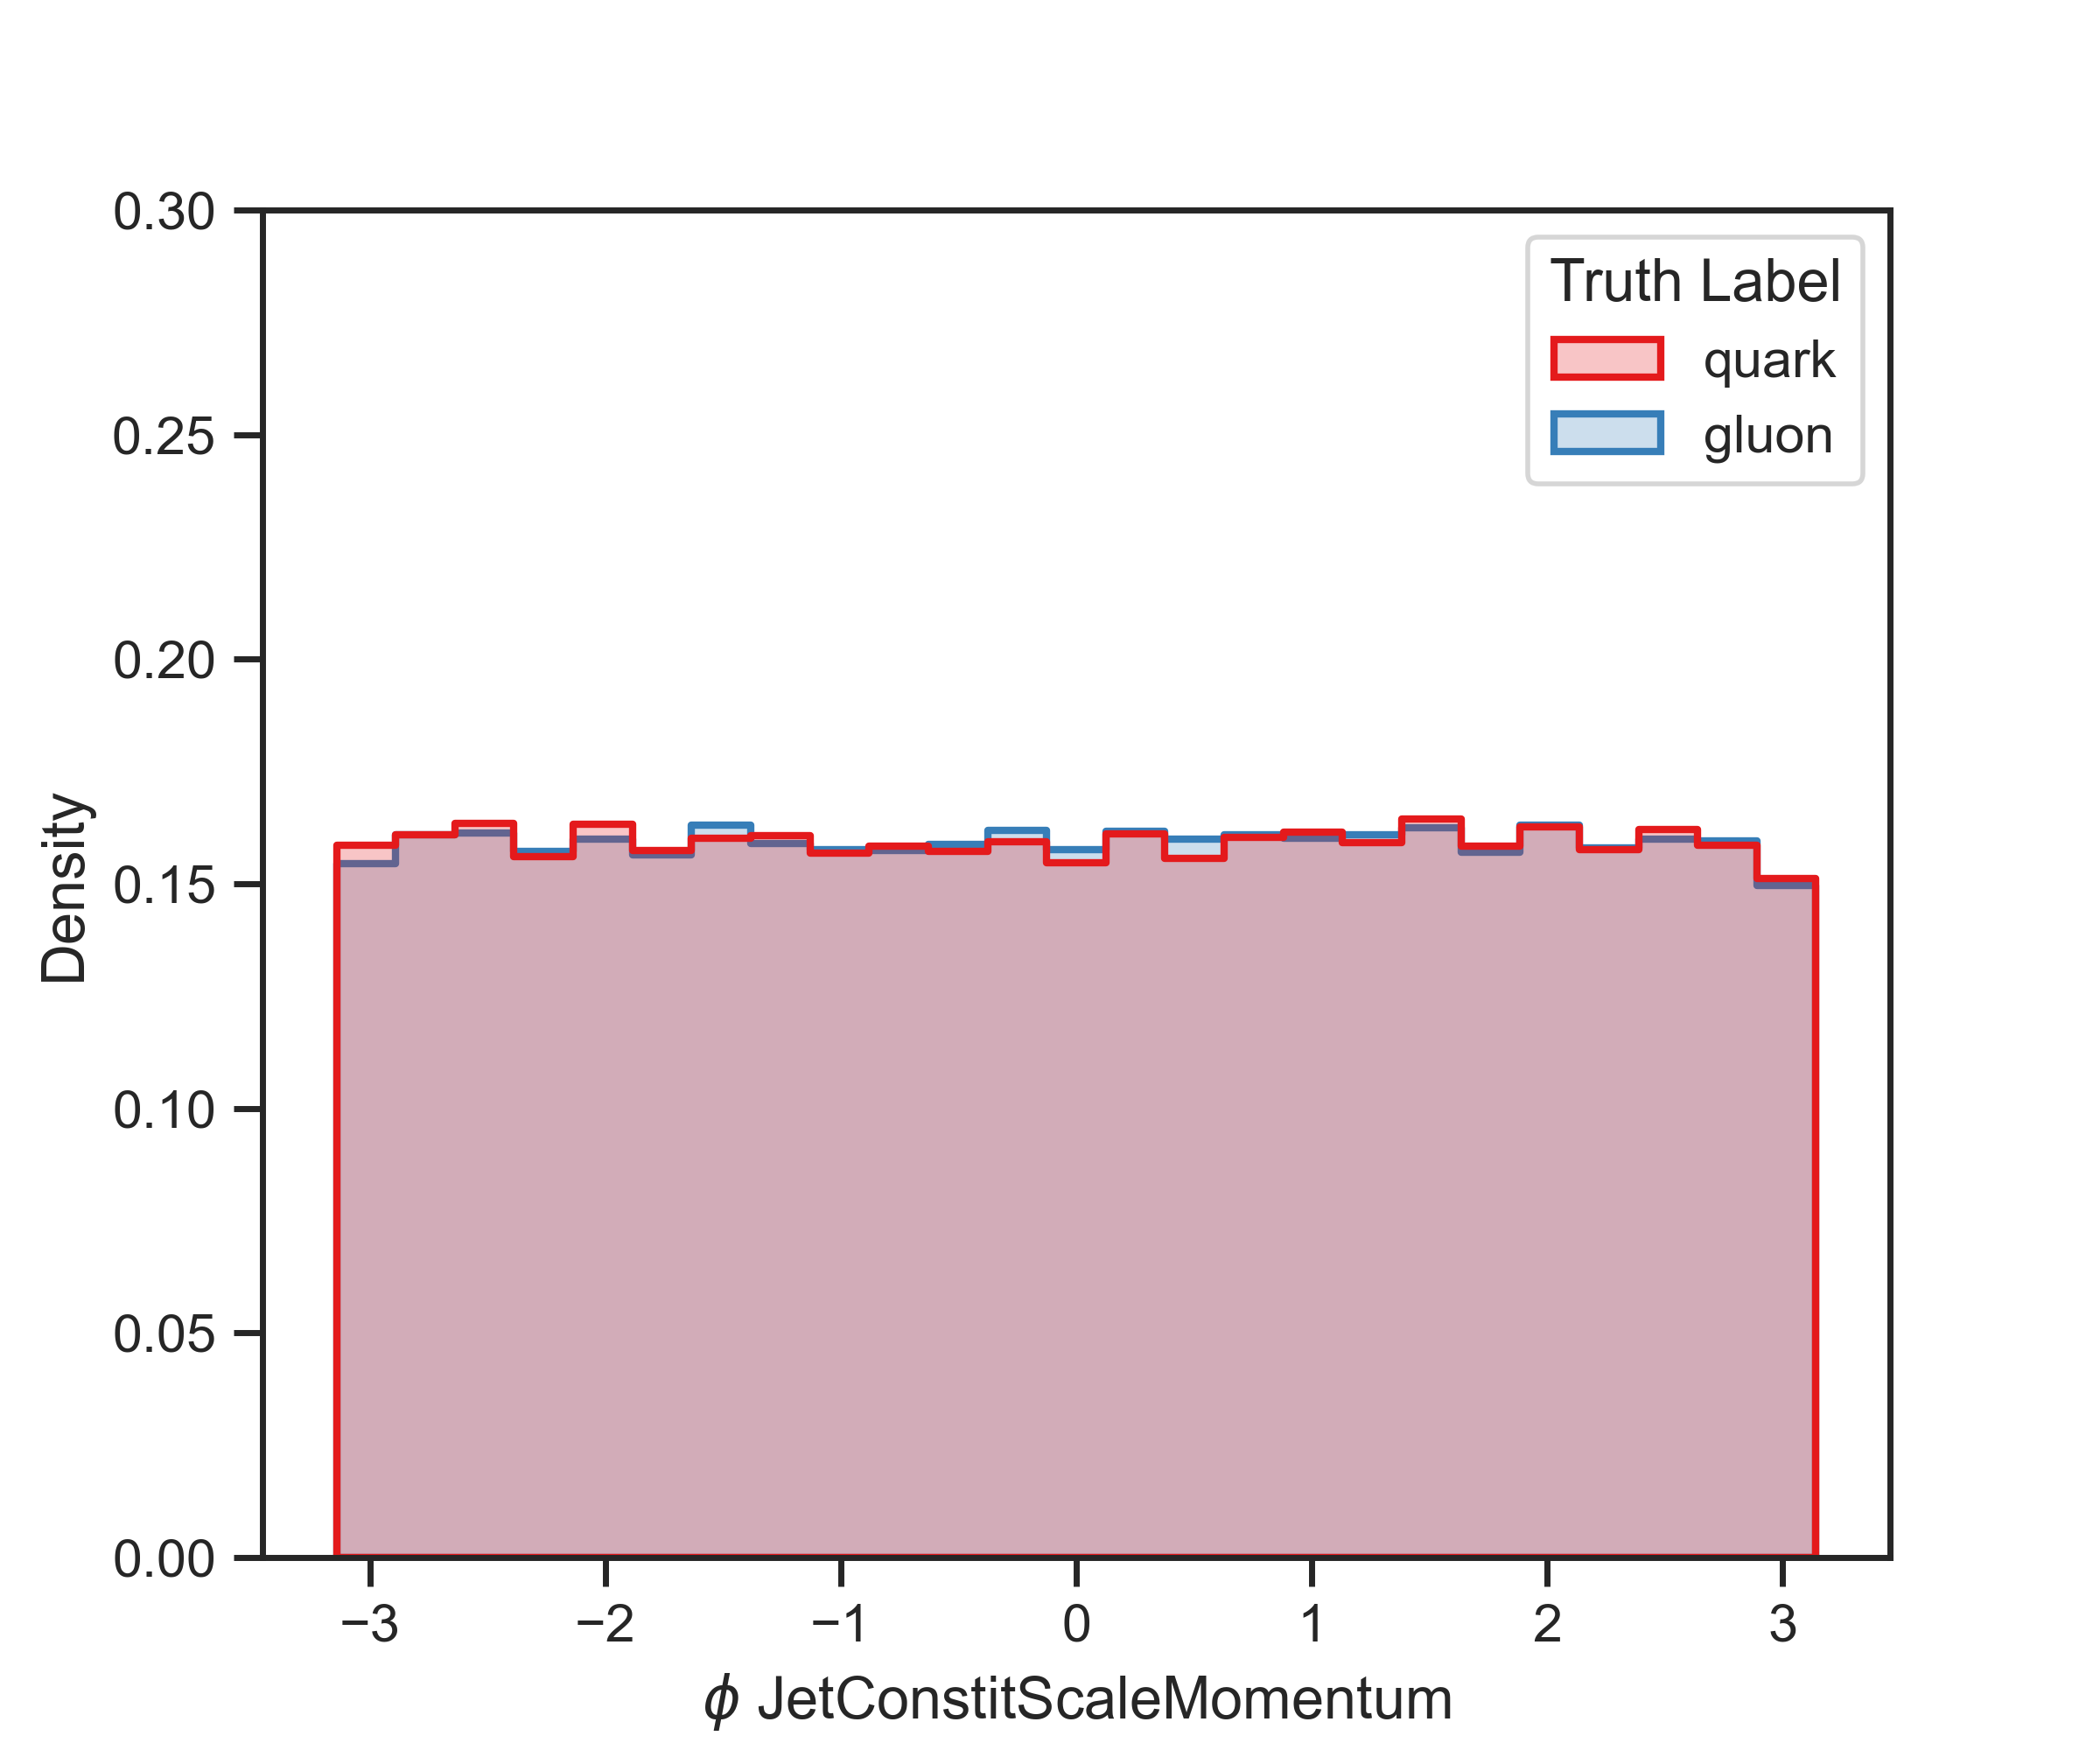
\includegraphics[width=1\textwidth]{src/plots/distributions/highlevel/jets_JetConstitScaleMomentum_phi.png}
		\caption{\texttt{jets\_JetConstitScaleMomentum\_phi}}
		\label{fig:highlevel_11}
	\end{subfigure}
\caption{High-level Jet Variables, part 2}
\label{fig:highlevel_6-11}
\end{figure}

\begin{figure}[!htb]
	\centering
	\begin{subfigure}[t]{0.48\textwidth}
		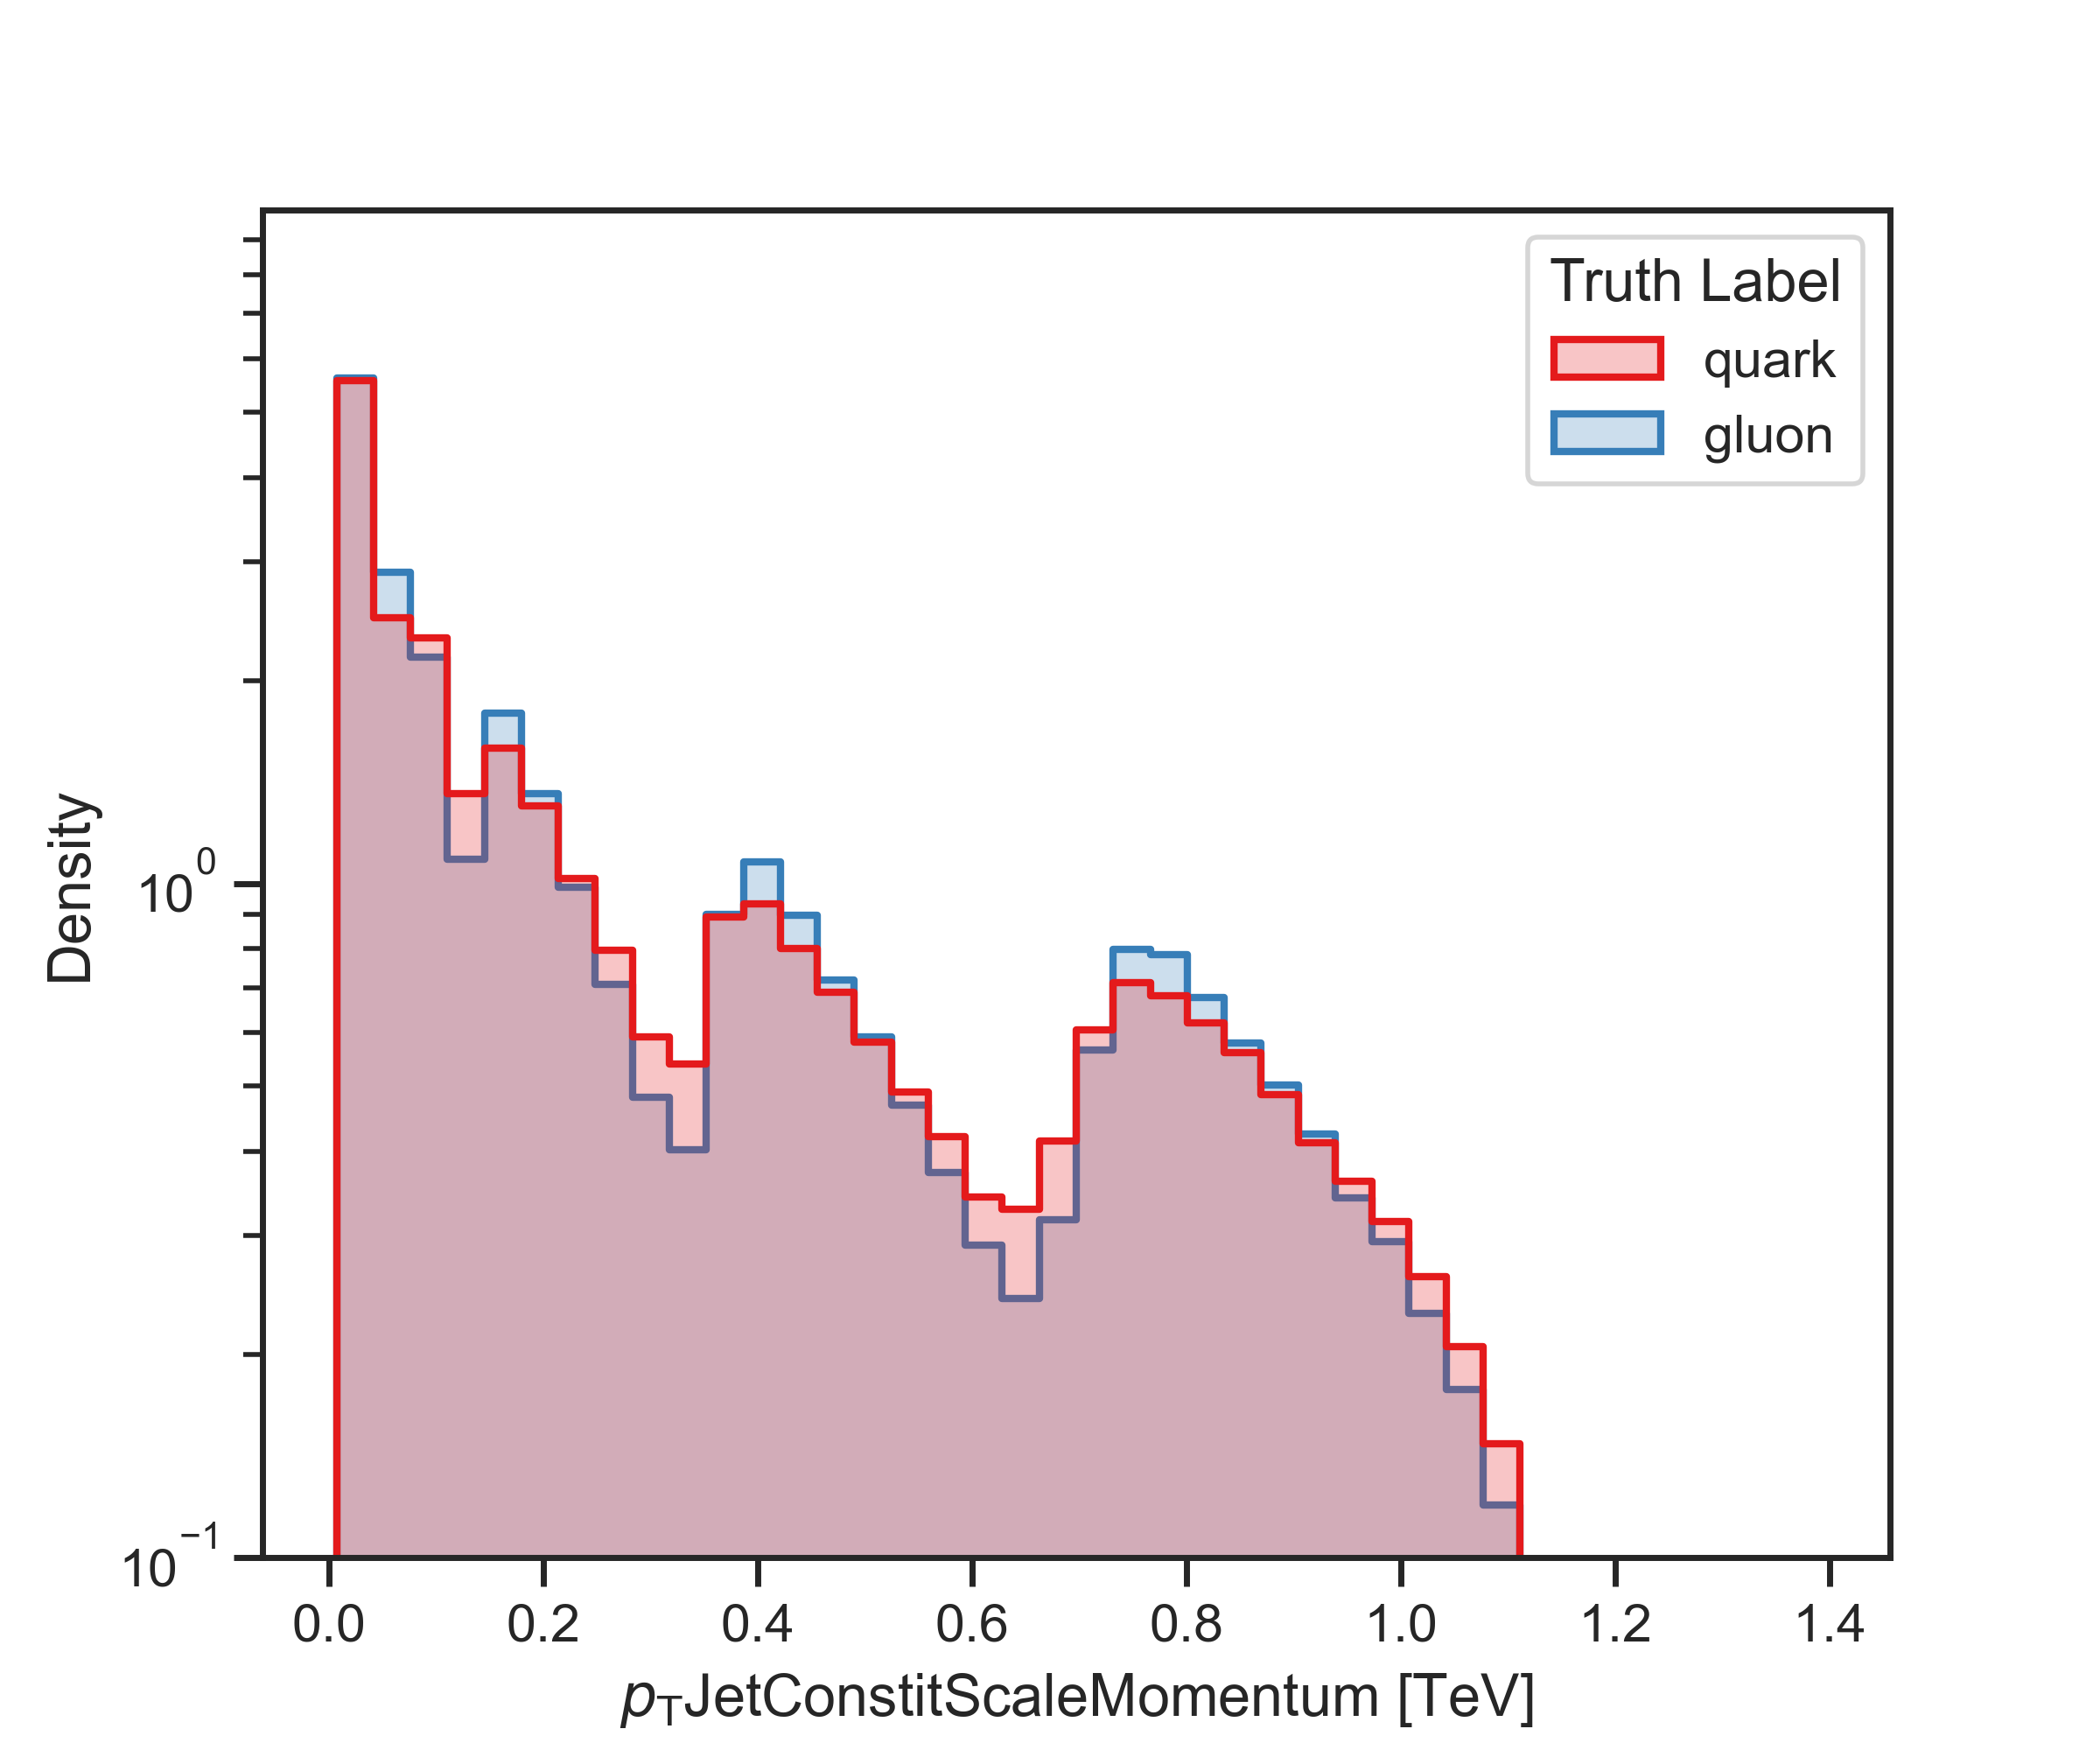
\includegraphics[width=1\textwidth]{src/plots/distributions/highlevel/jets_JetConstitScaleMomentum_pt.png}
		\caption{\texttt{jets\_JetConstitScaleMomentum\_pt}}
		\label{fig:highlevel_12}
	\end{subfigure}
	\begin{subfigure}[t]{0.48\textwidth}
		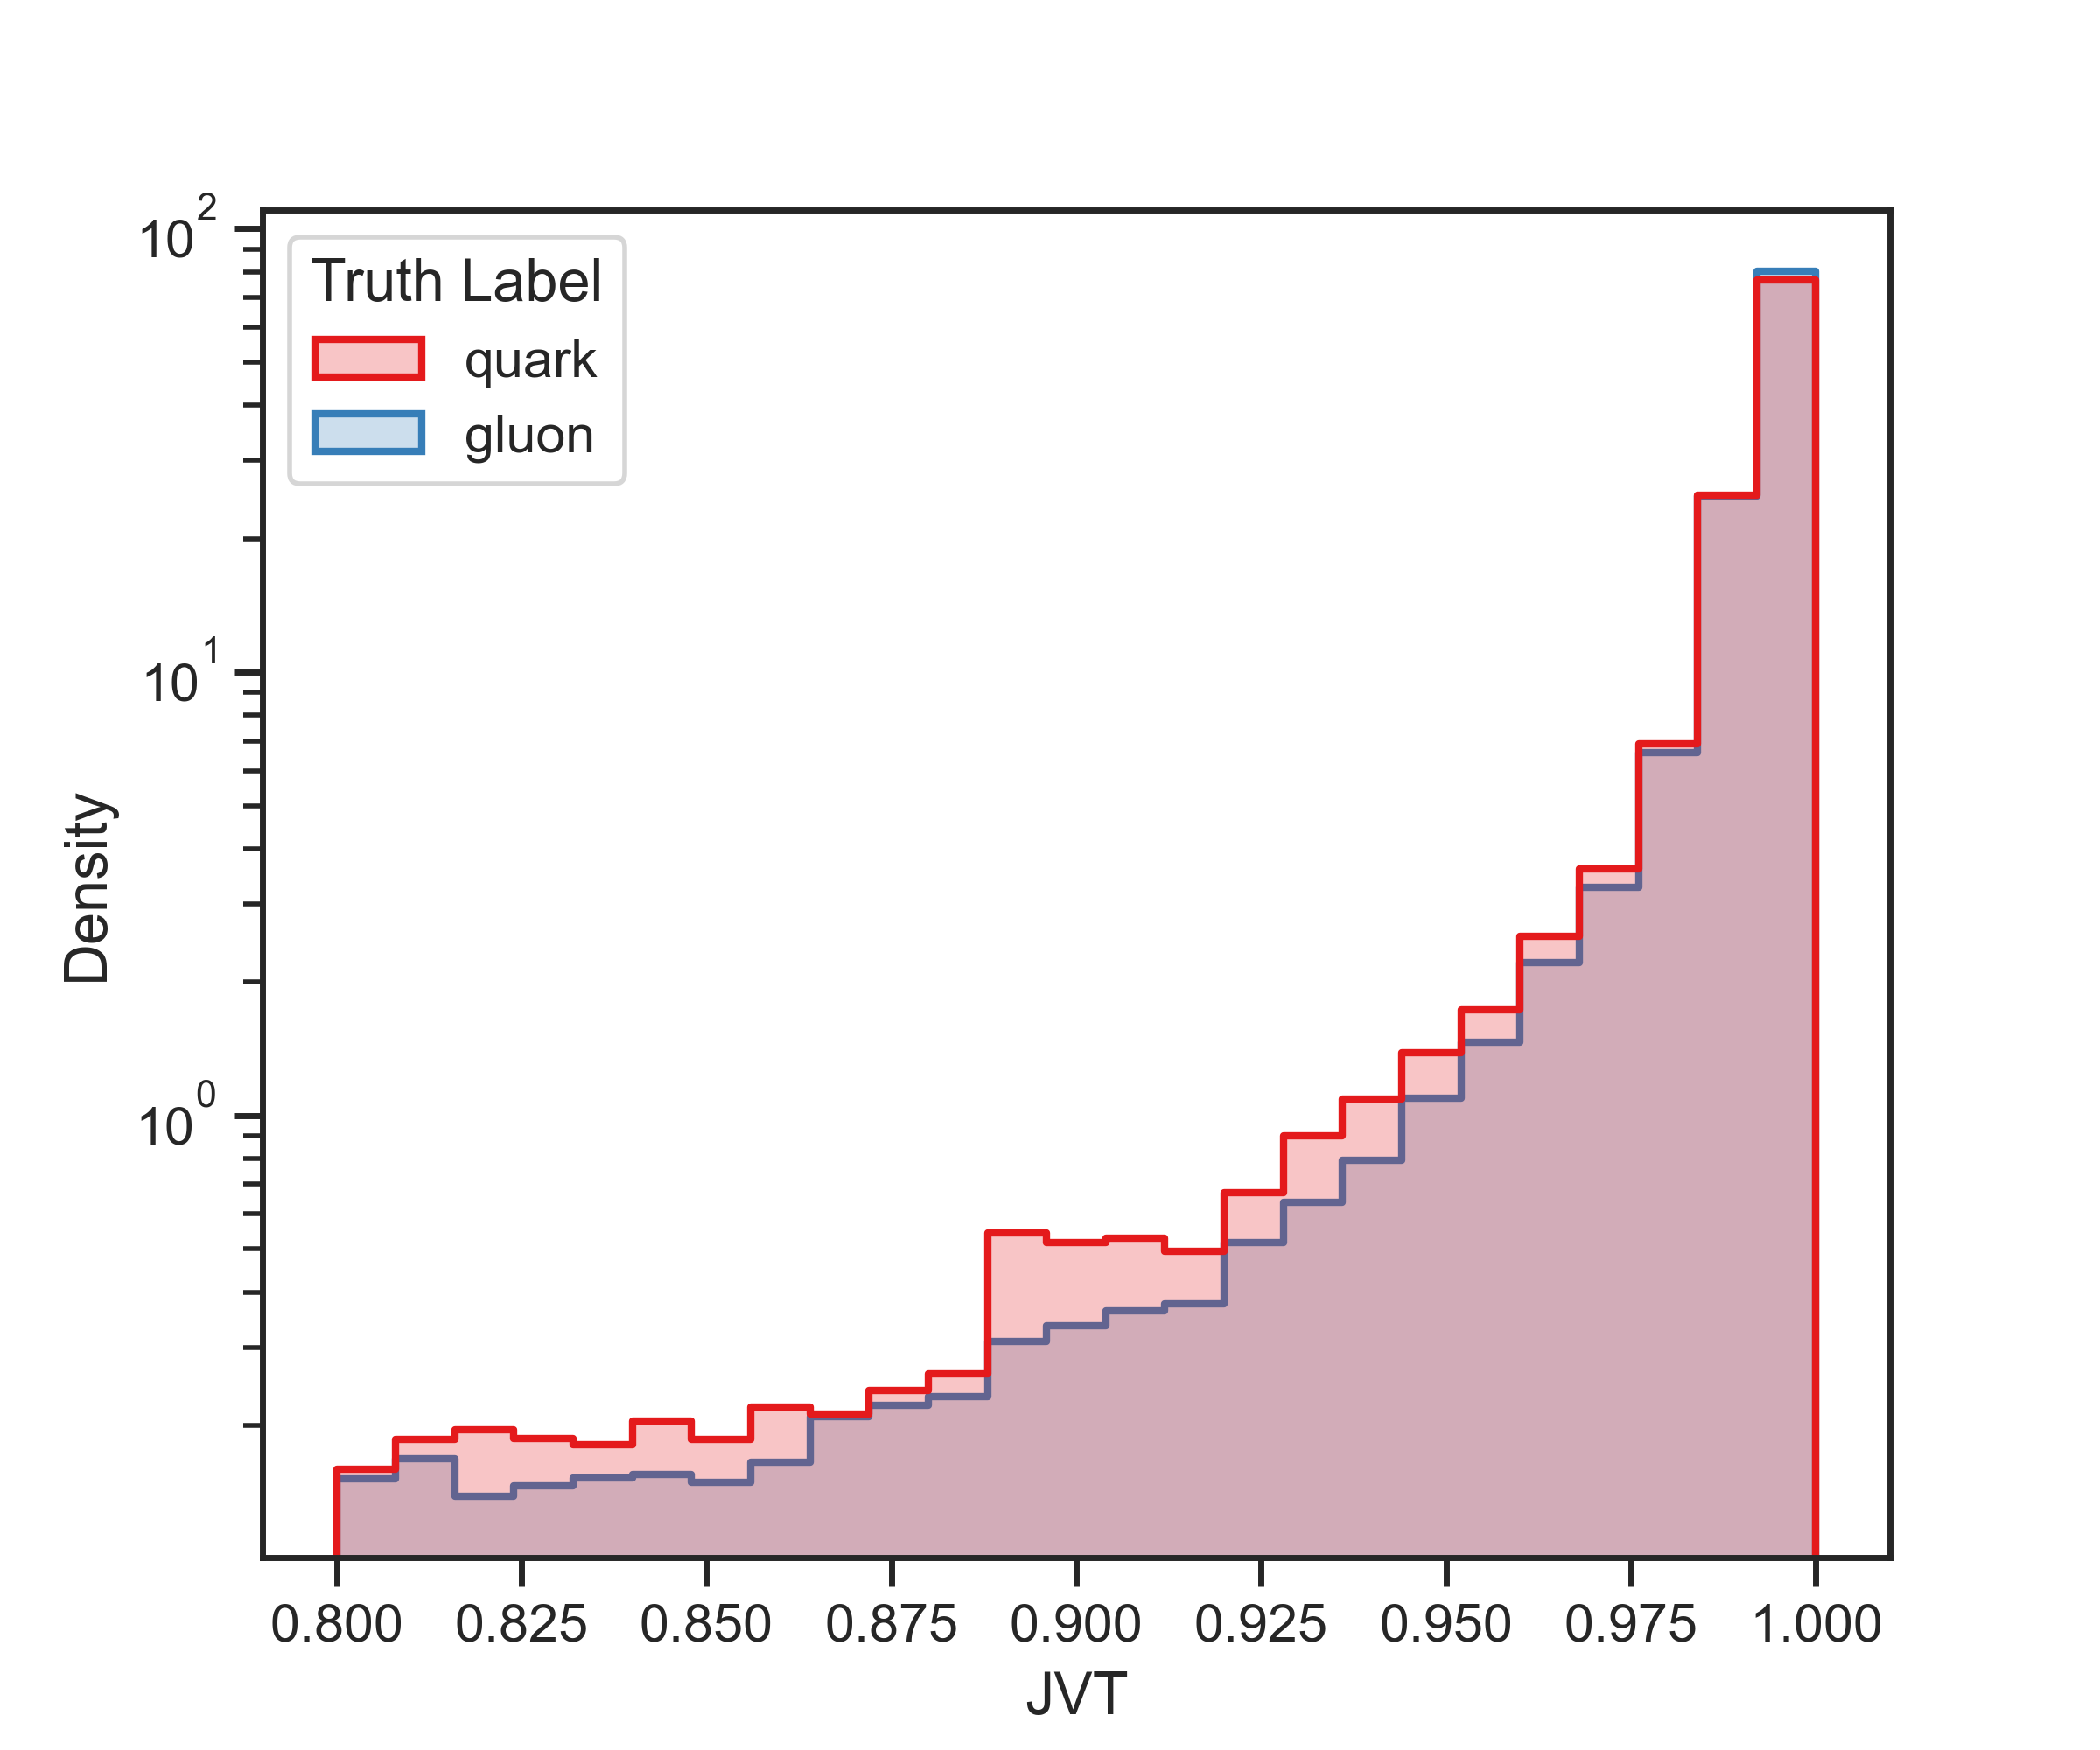
\includegraphics[width=1\textwidth]{src/plots/distributions/highlevel/jets_Jvt.png}
		\caption{\texttt{jets\_Jvt}}
		\label{fig:highlevel_13}
	\end{subfigure}
	\begin{subfigure}[t]{0.48\textwidth}
		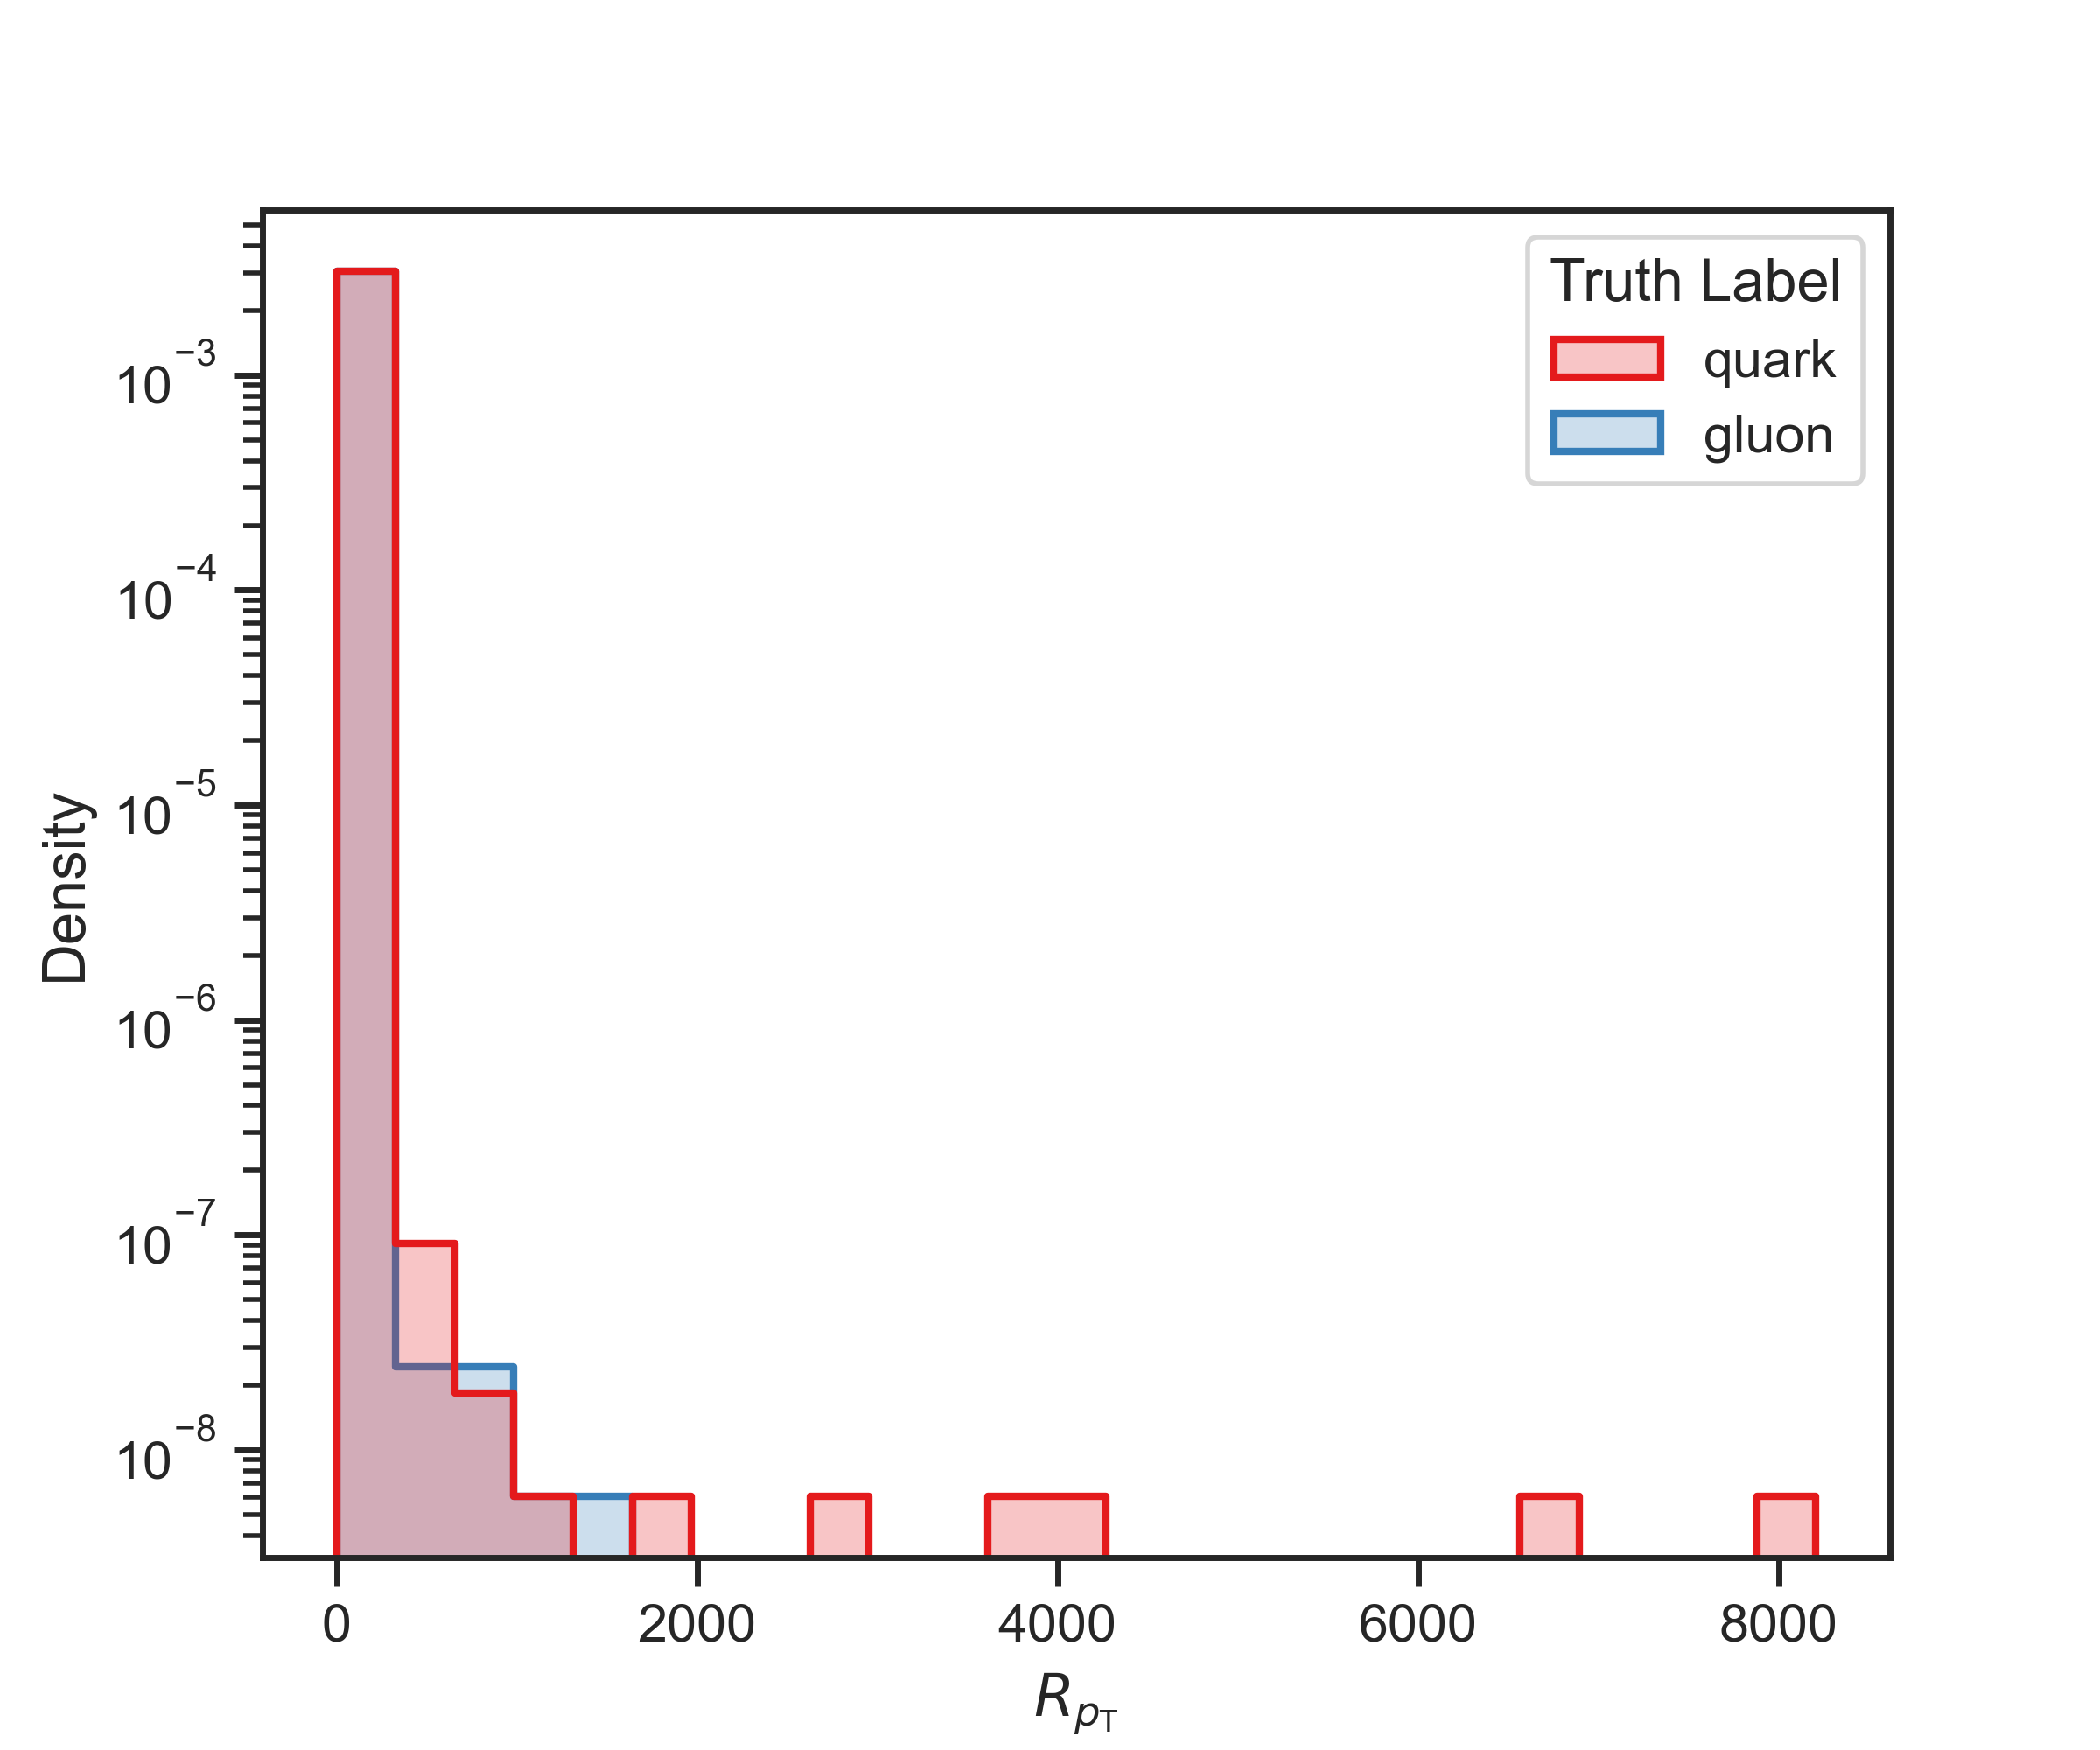
\includegraphics[width=1\textwidth]{src/plots/distributions/highlevel/jets_JvtRpt.png}
		\caption{\texttt{jets\_JvtRpt}}
		\label{fig:highlevel_14}
	\end{subfigure}
	\begin{subfigure}[t]{0.48\textwidth}
		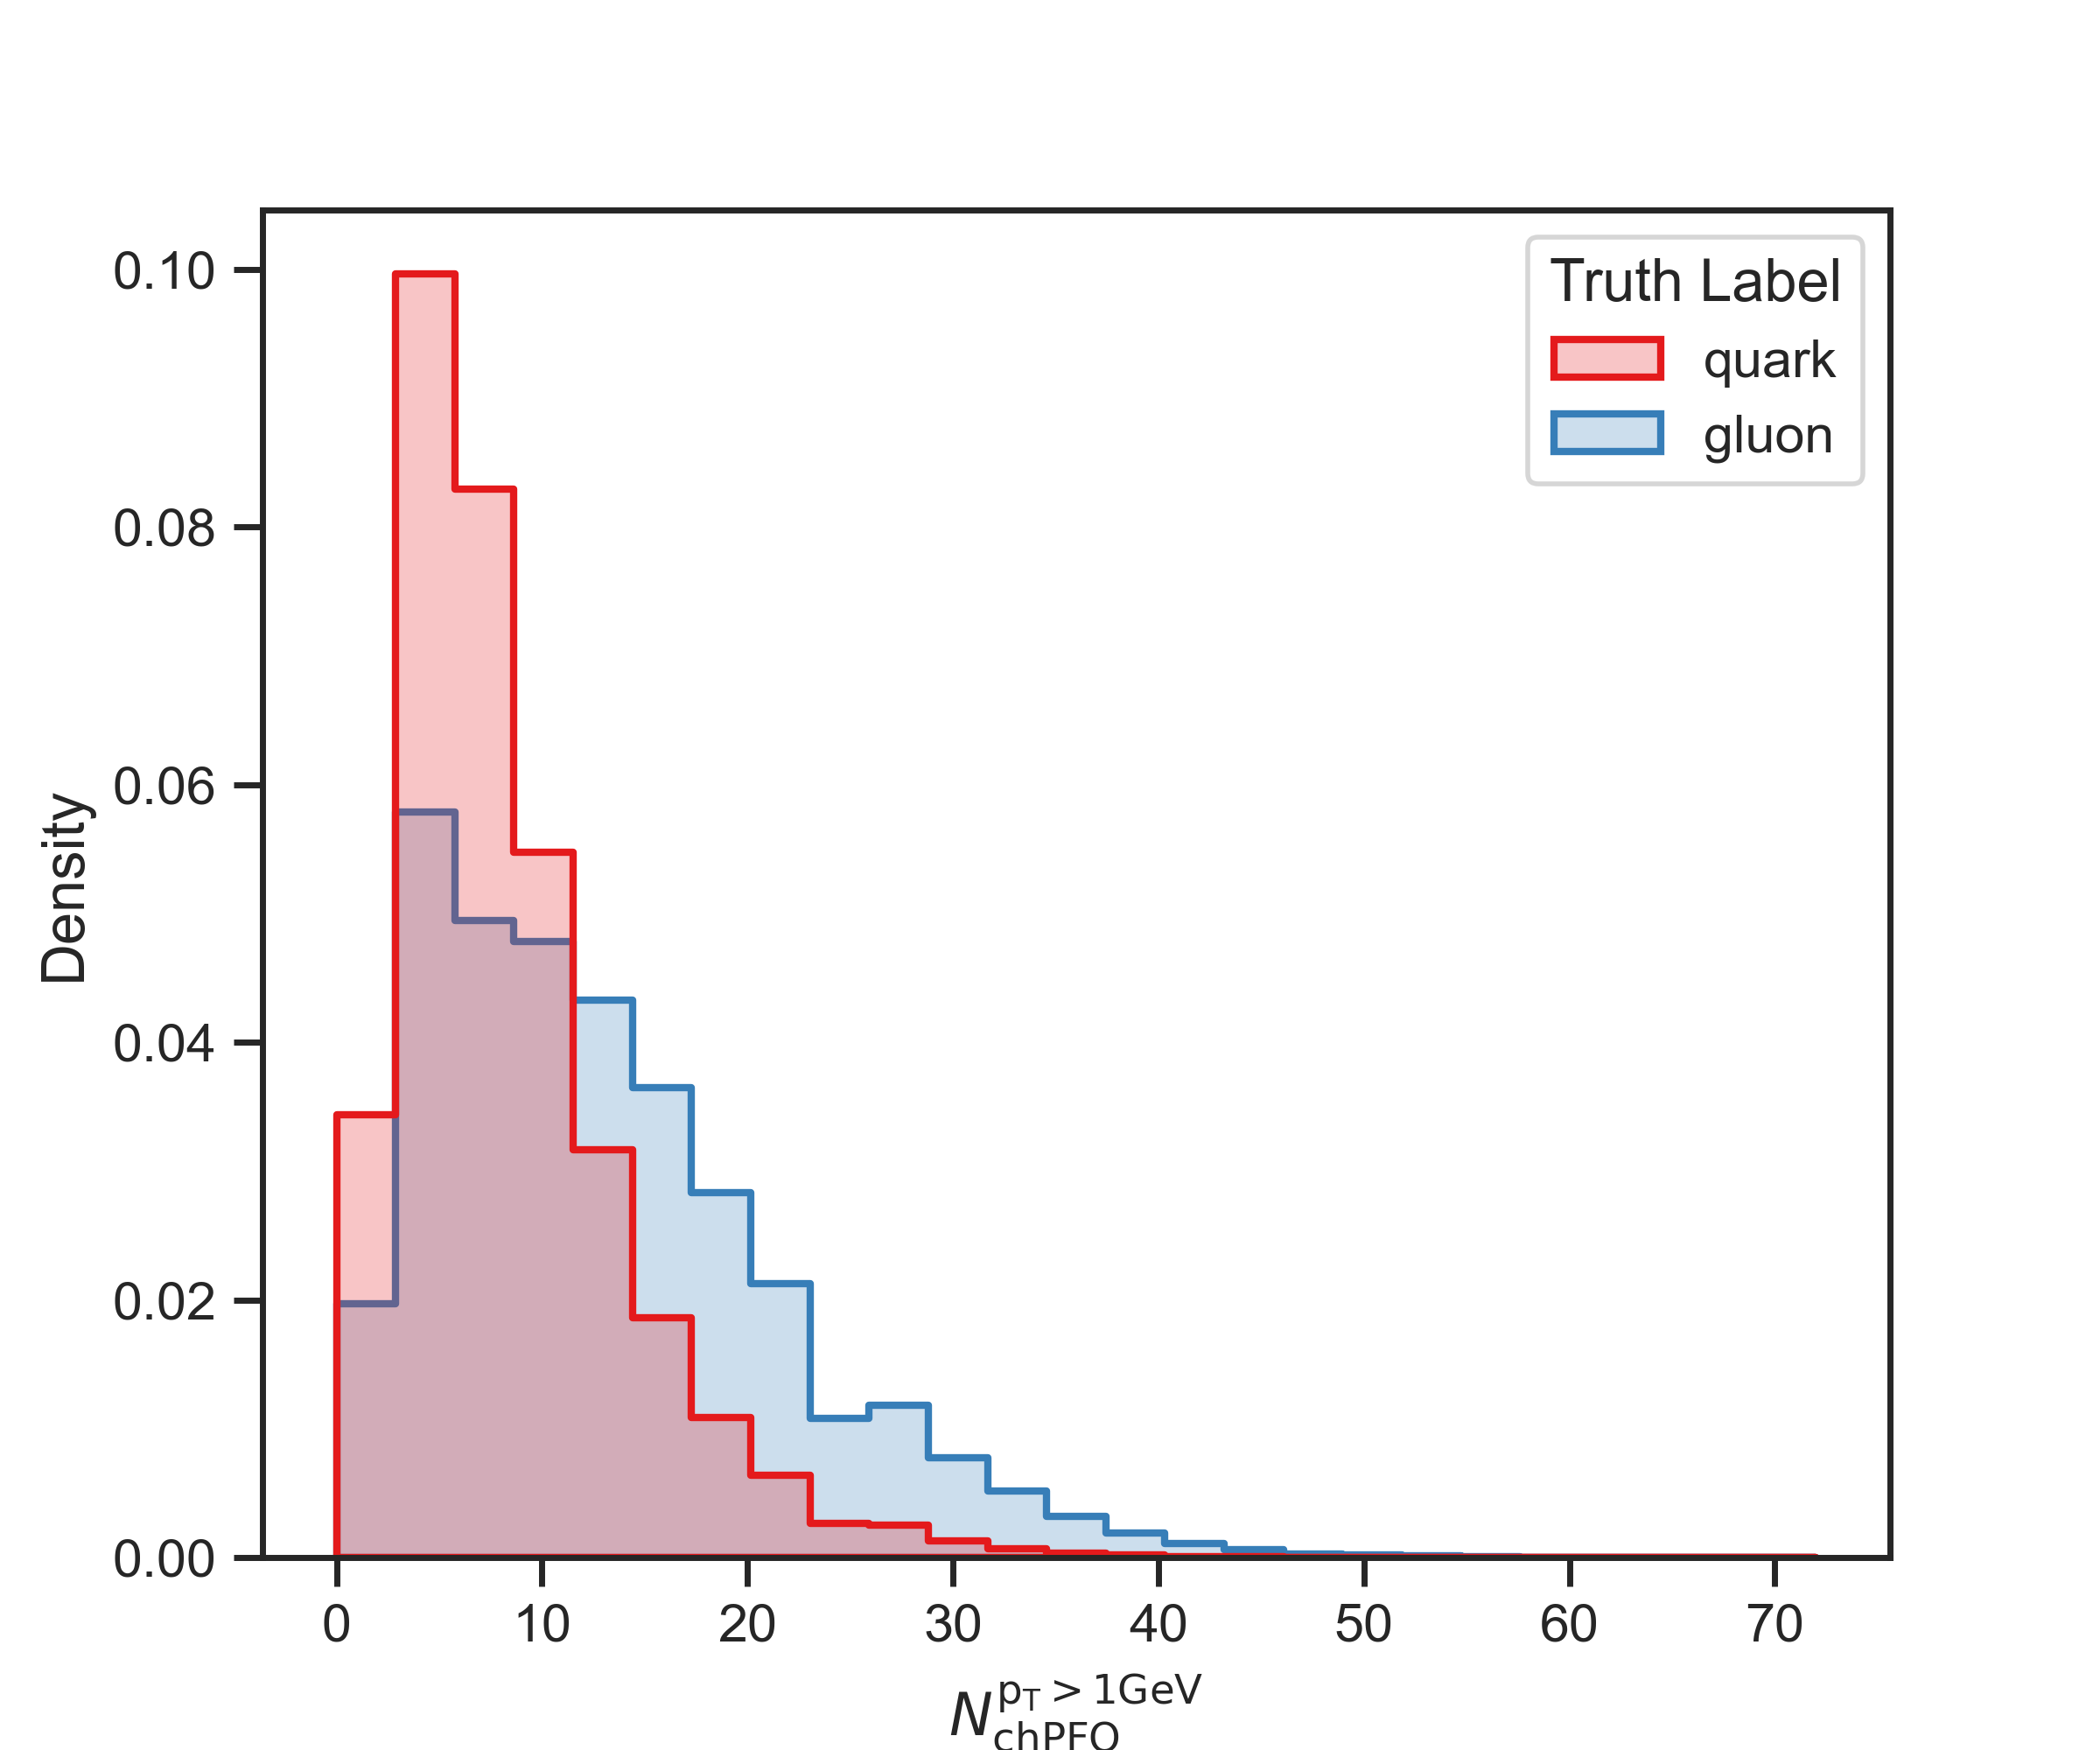
\includegraphics[width=1\textwidth]{src/plots/distributions/highlevel/jets_NumChargedPFOPt1000[0].png}
		\caption{\texttt{jets\_NumChargedPFOPt1000[0]}}
		\label{fig:highlevel_15}
	\end{subfigure}
	\begin{subfigure}[t]{0.48\textwidth}
		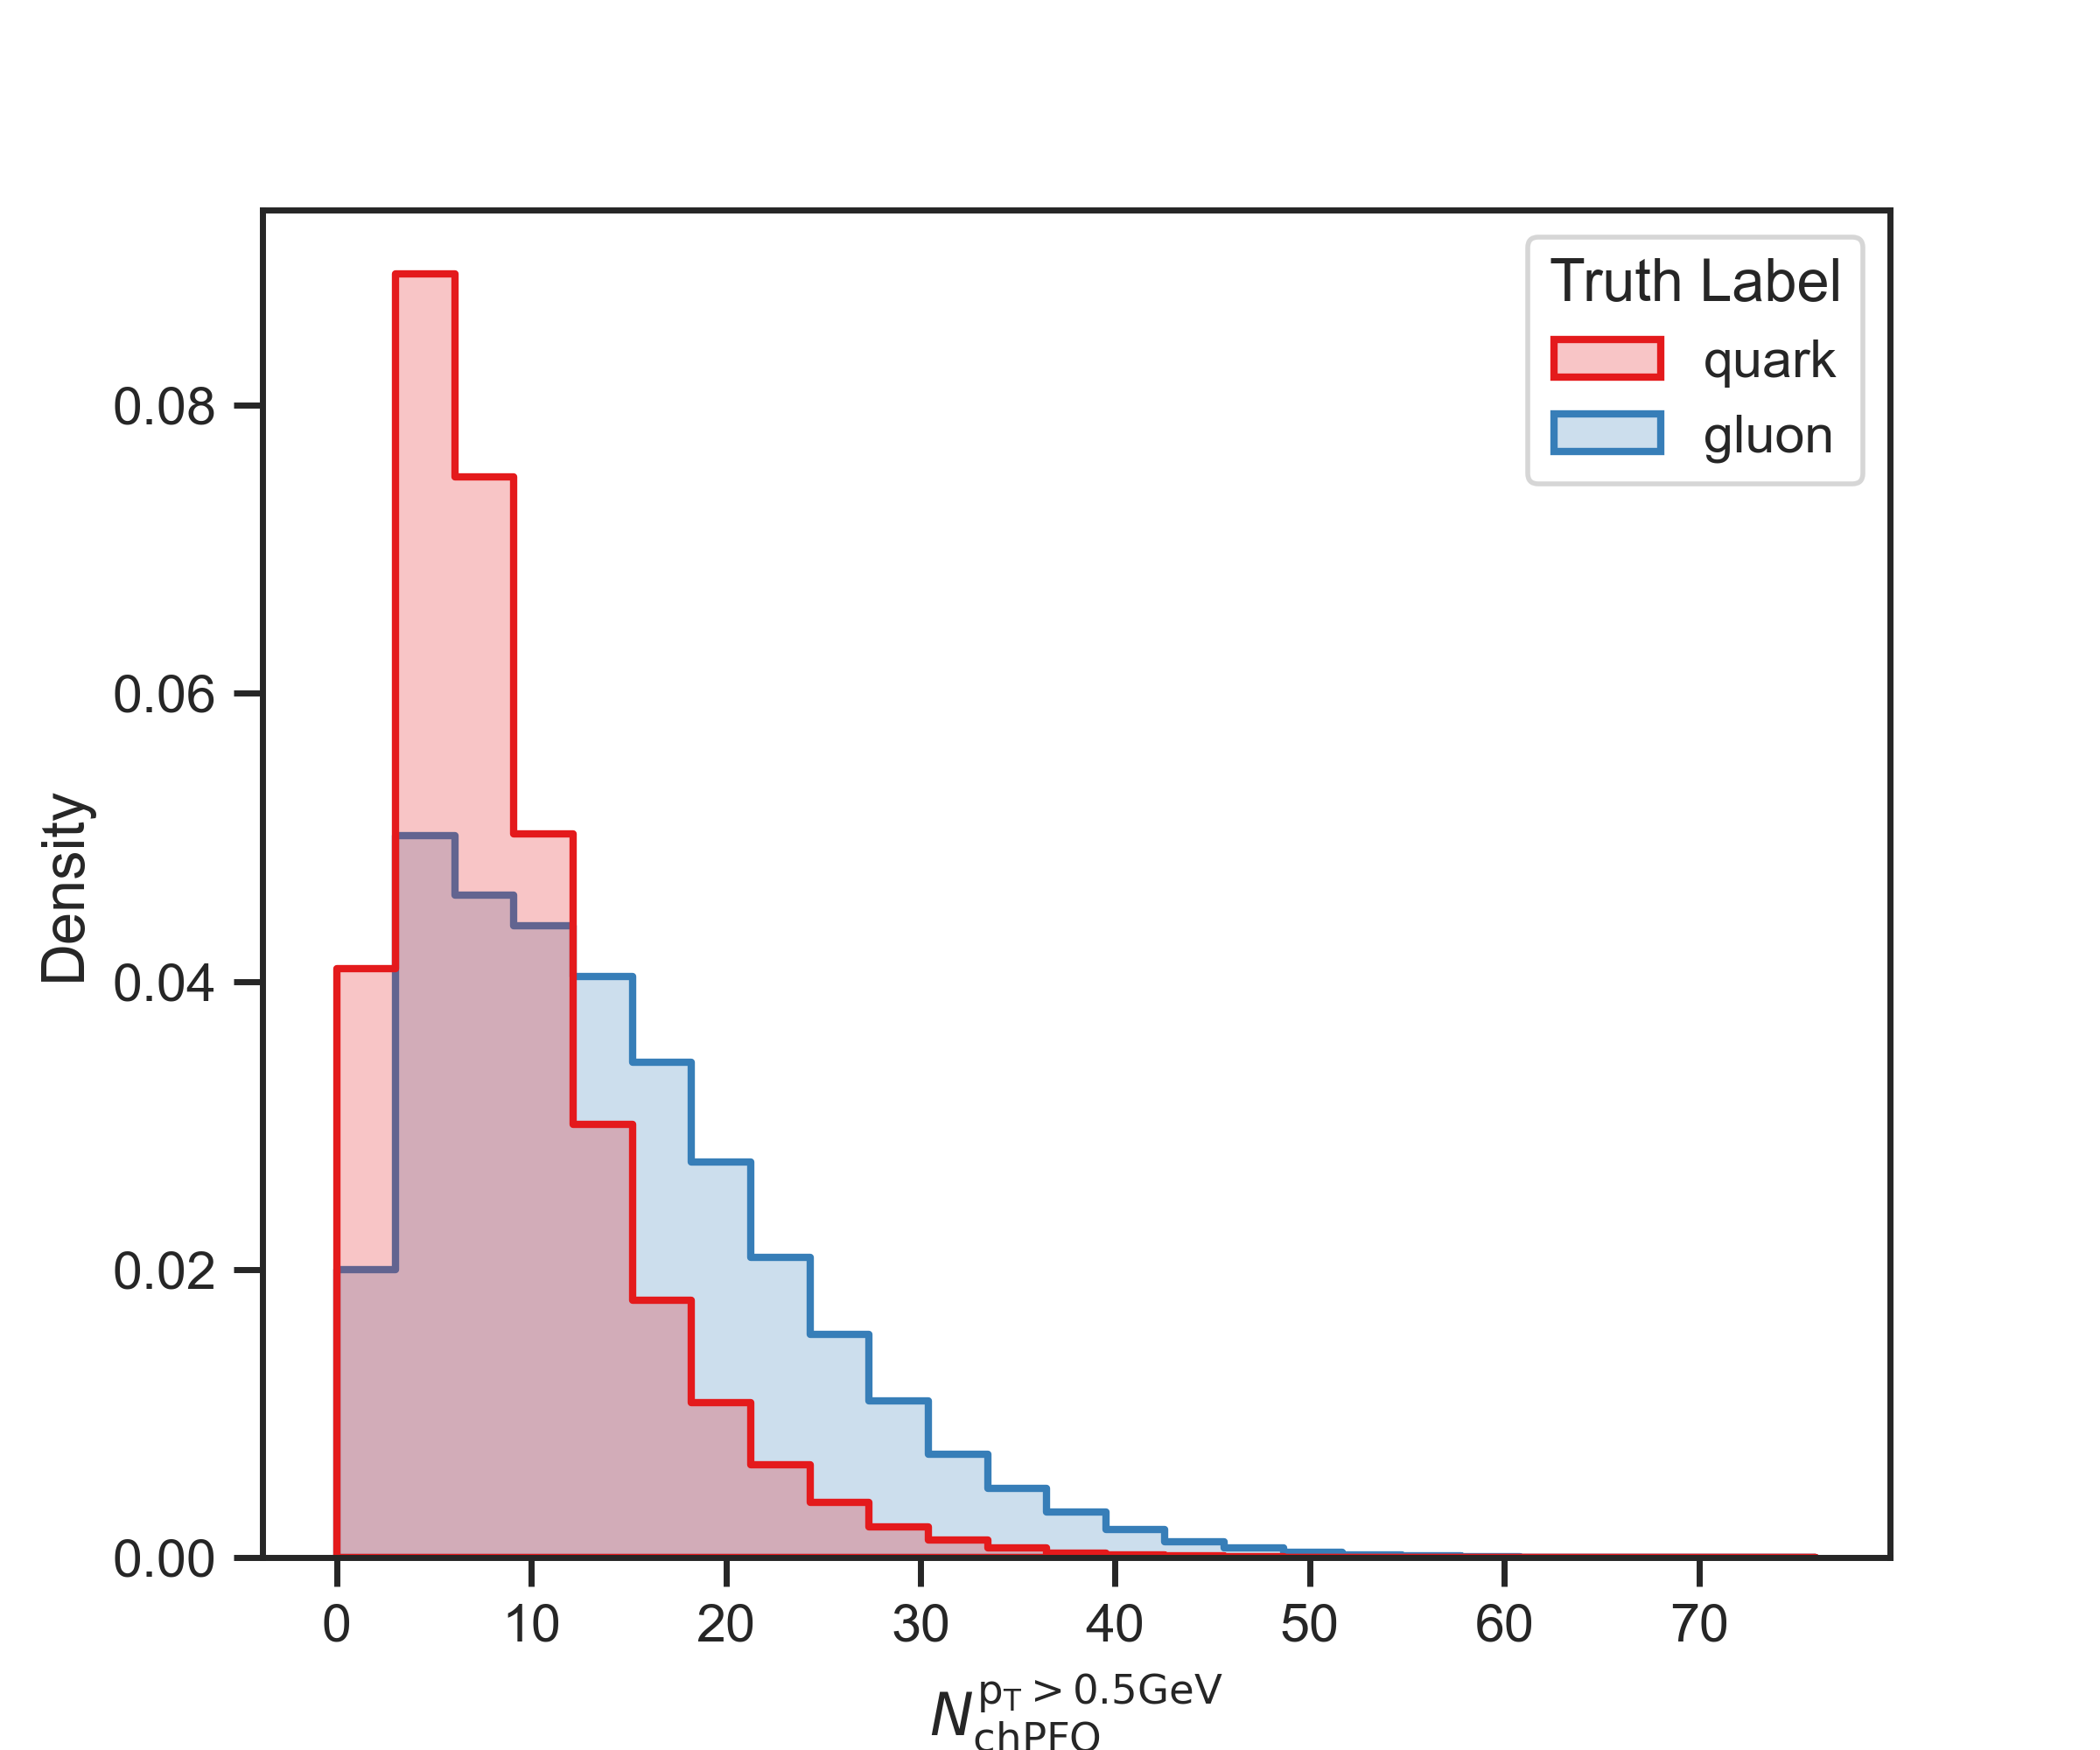
\includegraphics[width=1\textwidth]{src/plots/distributions/highlevel/jets_NumChargedPFOPt500[0].png}
		\caption{\texttt{jets\_NumChargedPFOPt500[0]}}
		\label{fig:highlevel_16}
	\end{subfigure}
	\begin{subfigure}[t]{0.48\textwidth}
		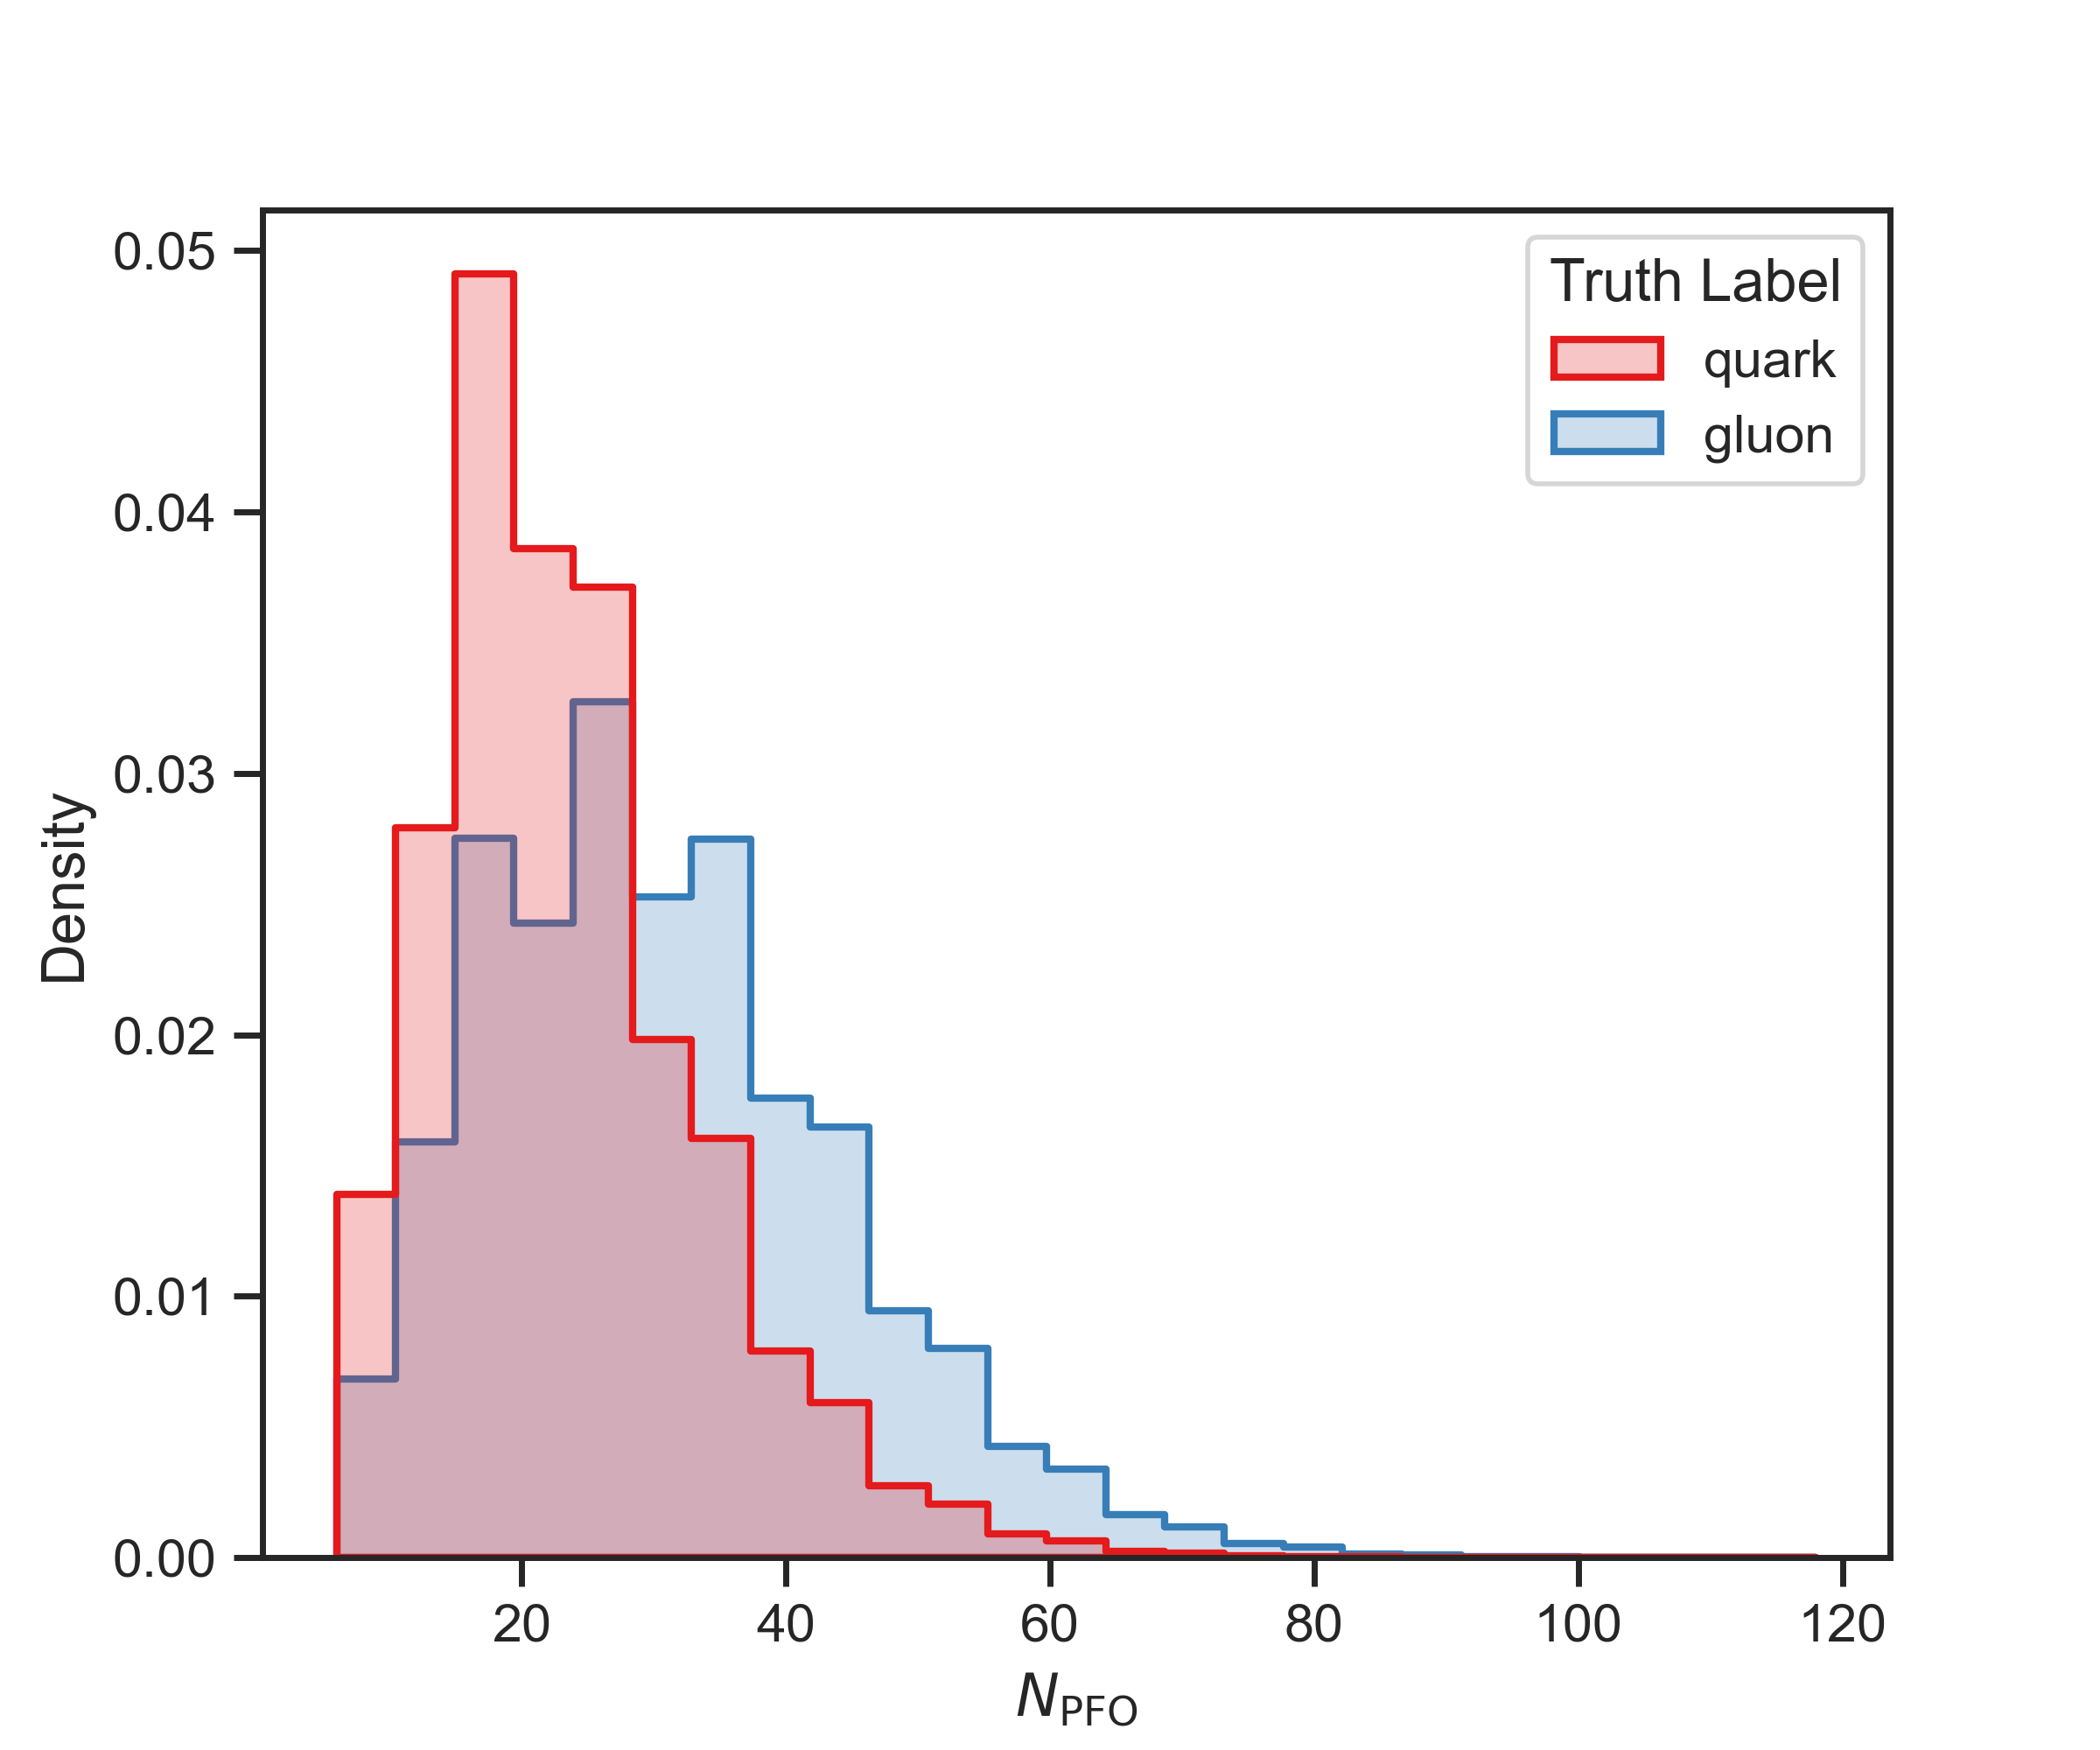
\includegraphics[width=1\textwidth]{src/plots/distributions/highlevel/jets_PFO_n.png}
		\caption{\texttt{jets\_PFO\_n}}
		\label{fig:highlevel_17}
	\end{subfigure}
\caption{High-level Jet Variables, part 3}
\label{fig:highlevel_12-17}
\end{figure}

\begin{figure}[!htb]
	\centering
	\begin{subfigure}[t]{0.48\textwidth}
		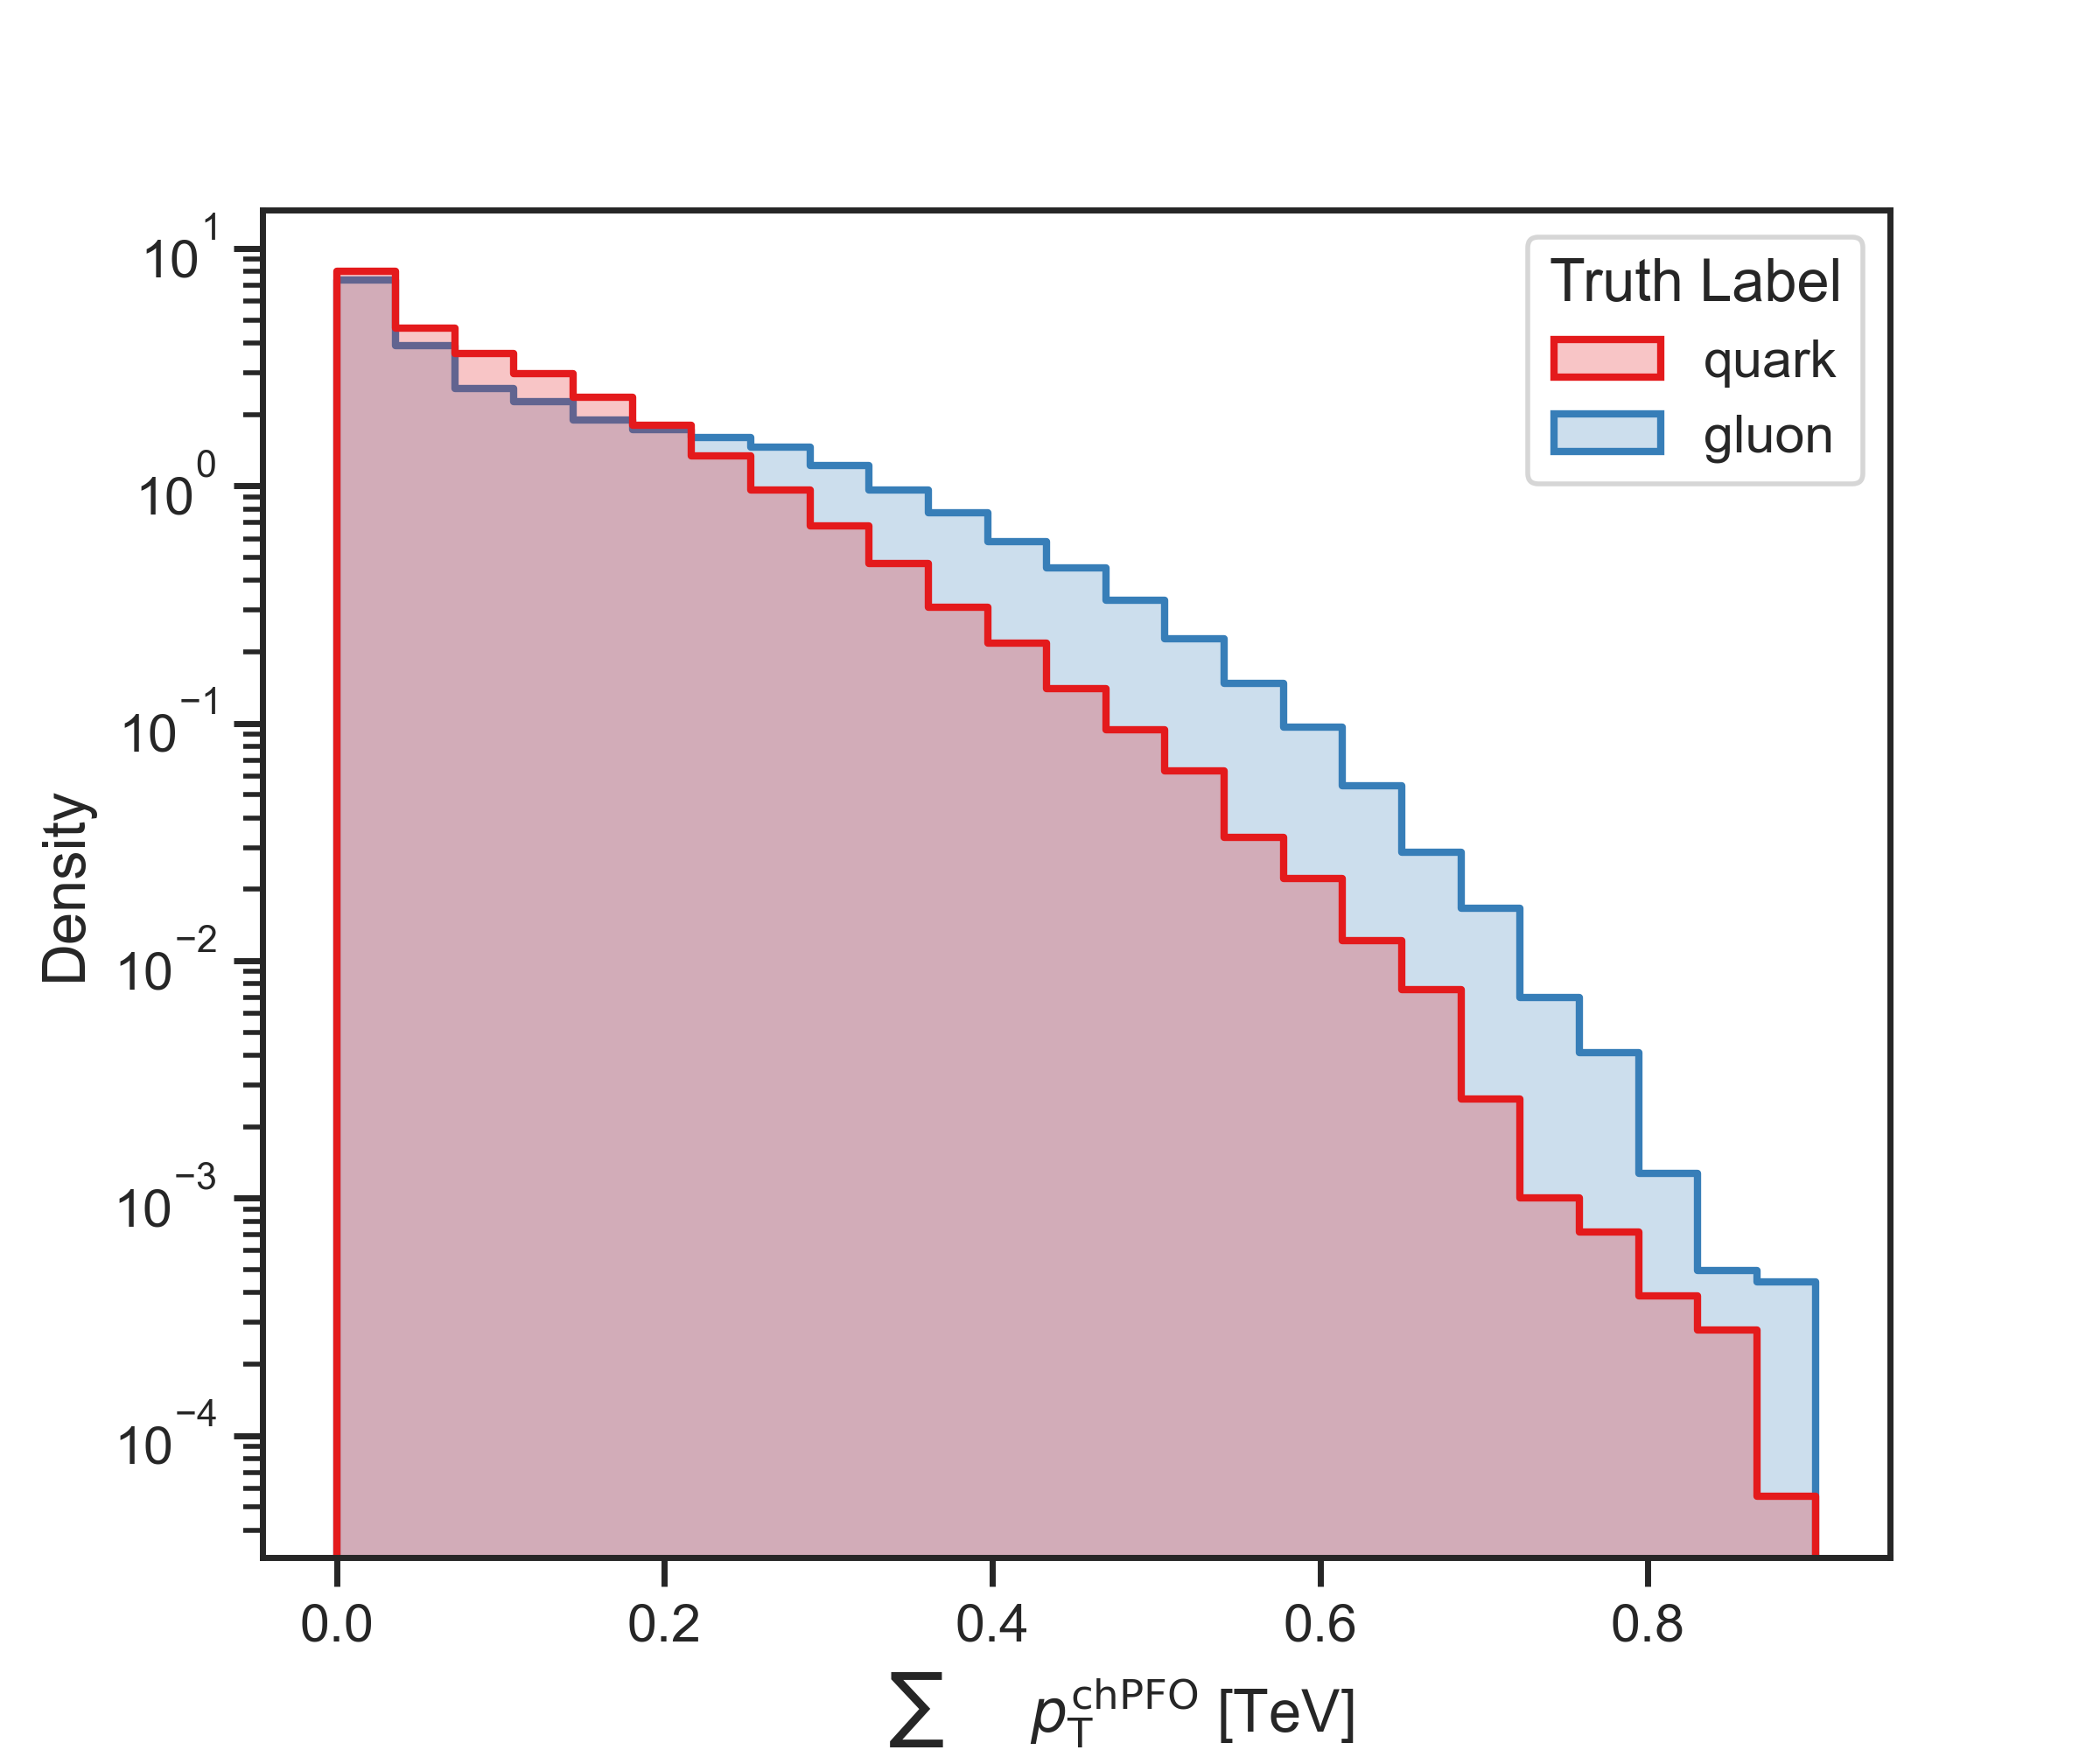
\includegraphics[width=1\textwidth]{src/plots/distributions/highlevel/jets_SumPtChargedPFOPt500[0].png}
		\caption{\texttt{jets\_SumPtChargedPFOPt500[0]}}
		\label{fig:highlevel_18}
	\end{subfigure}
	\begin{subfigure}[t]{0.48\textwidth}
		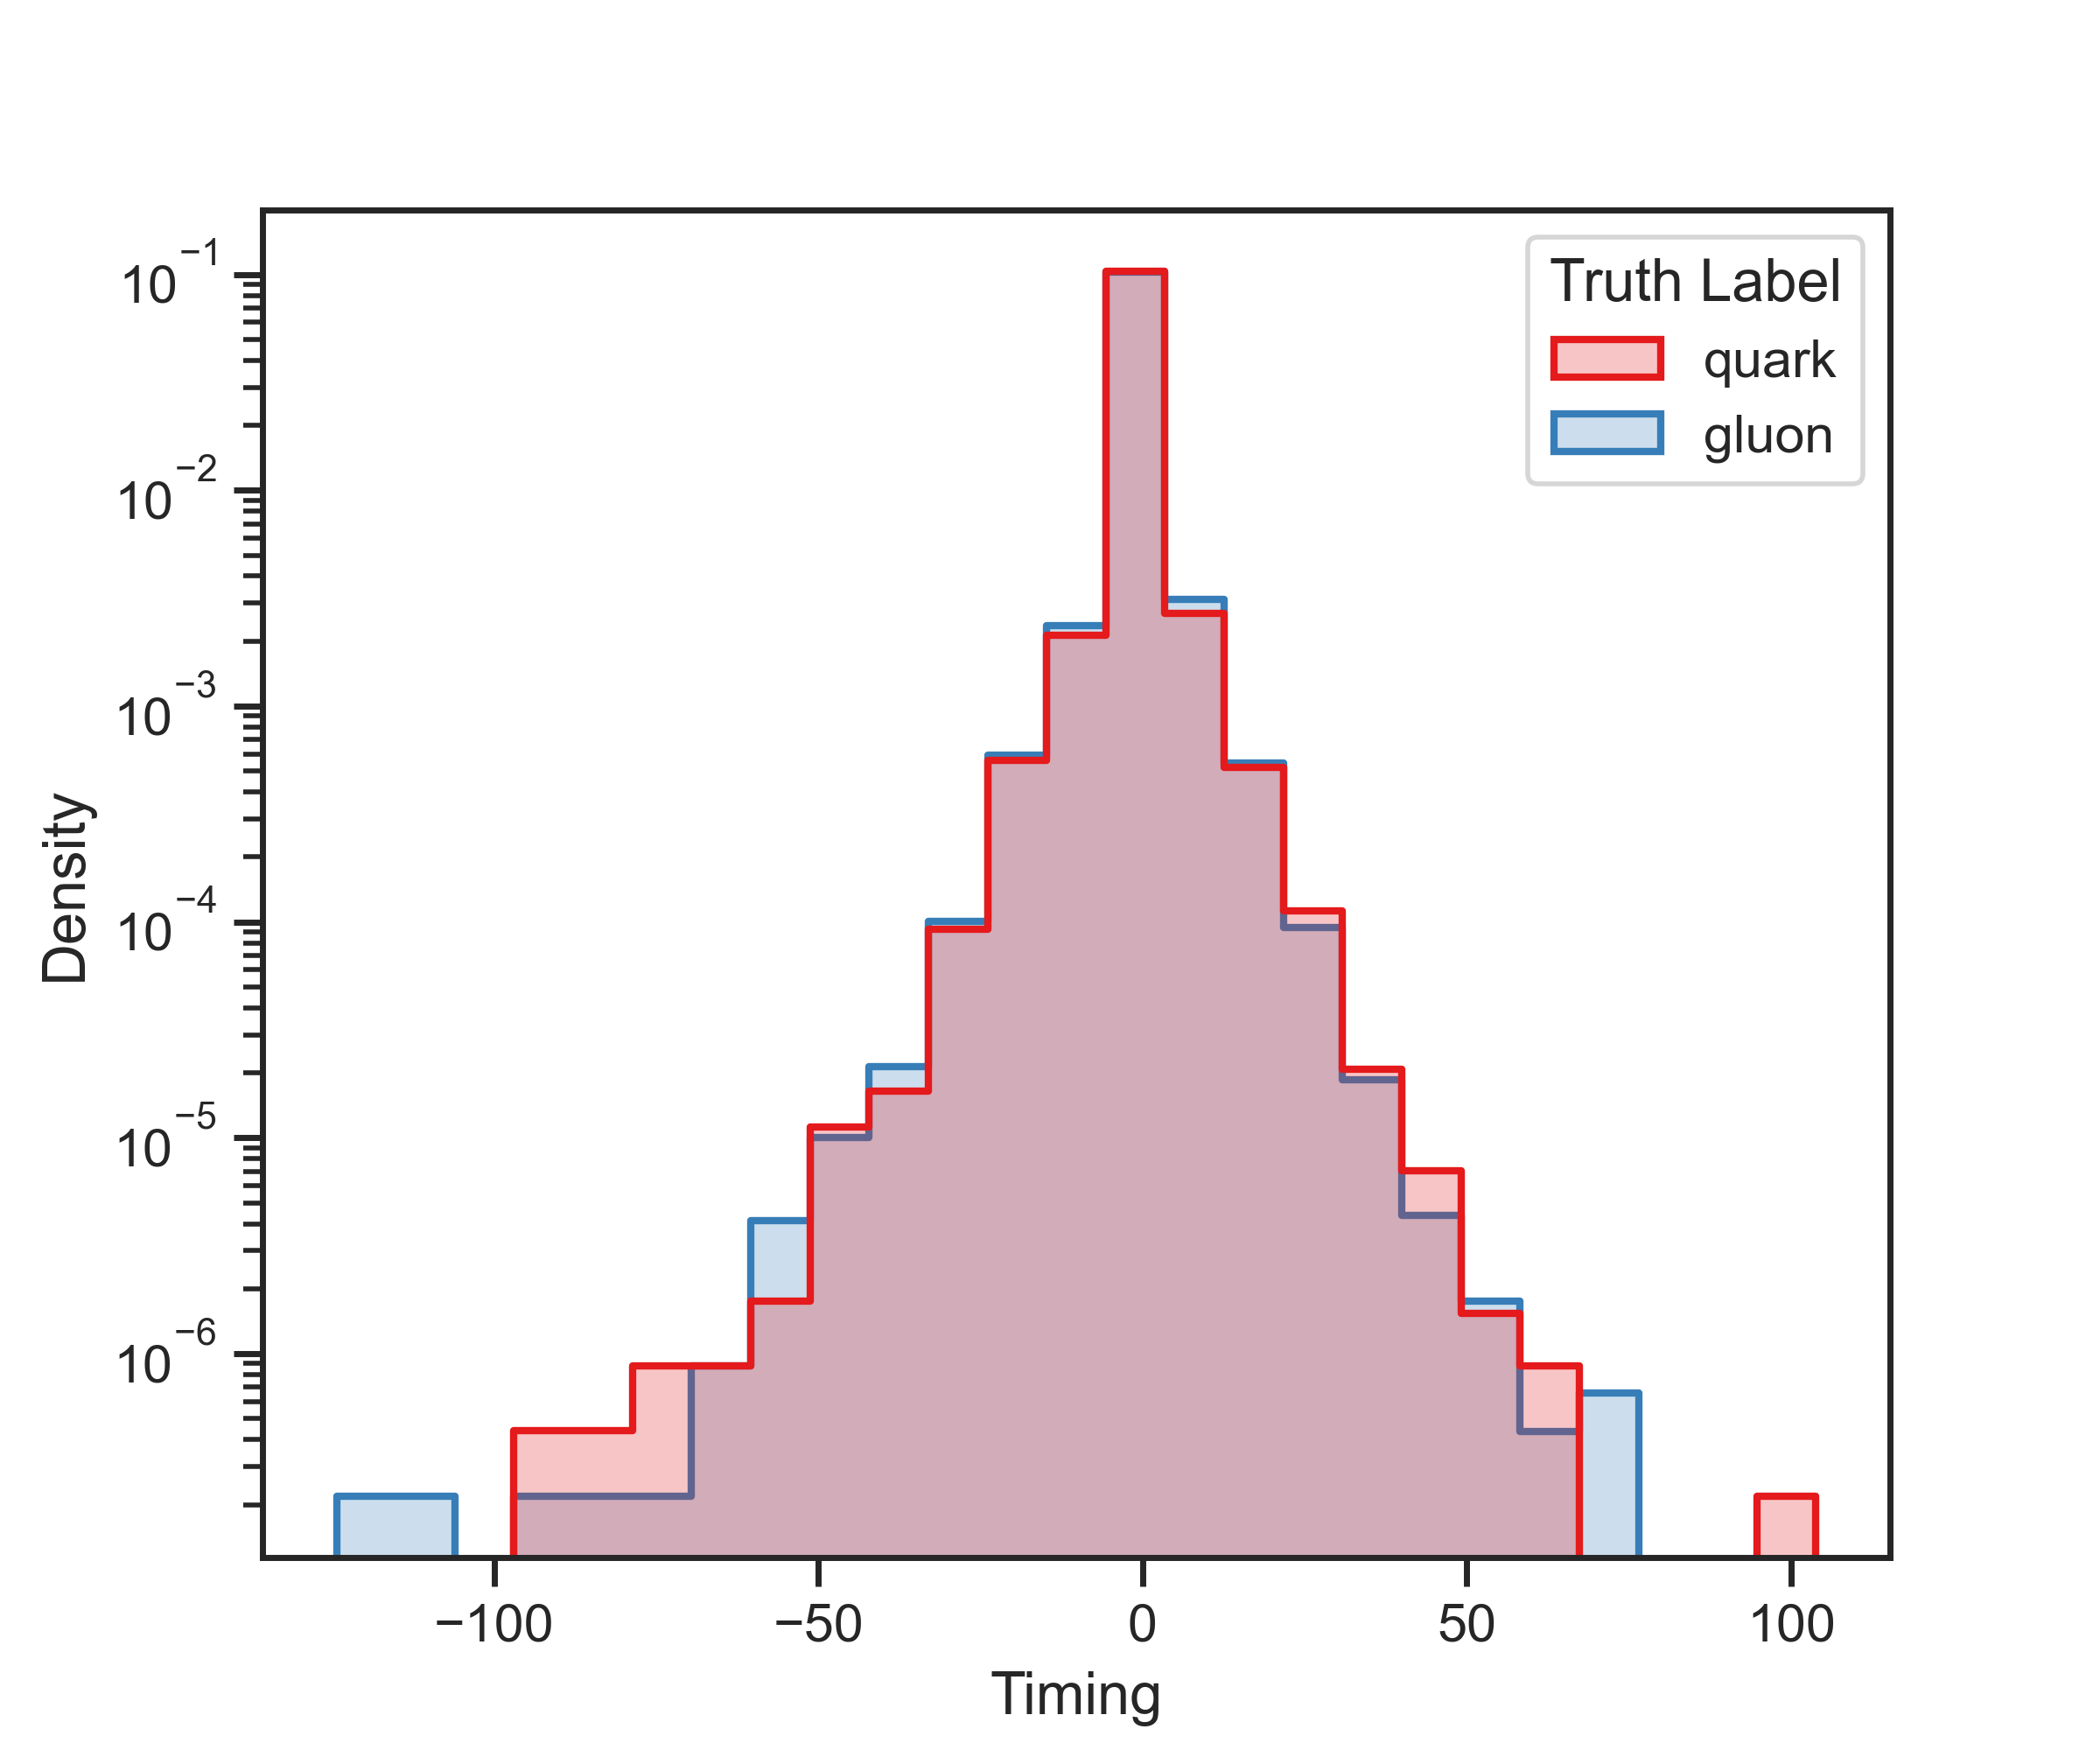
\includegraphics[width=1\textwidth]{src/plots/distributions/highlevel/jets_Timing.png}
		\caption{\texttt{jets\_Timing}}
		\label{fig:highlevel_19}
	\end{subfigure}
	\begin{subfigure}[t]{0.48\textwidth}
		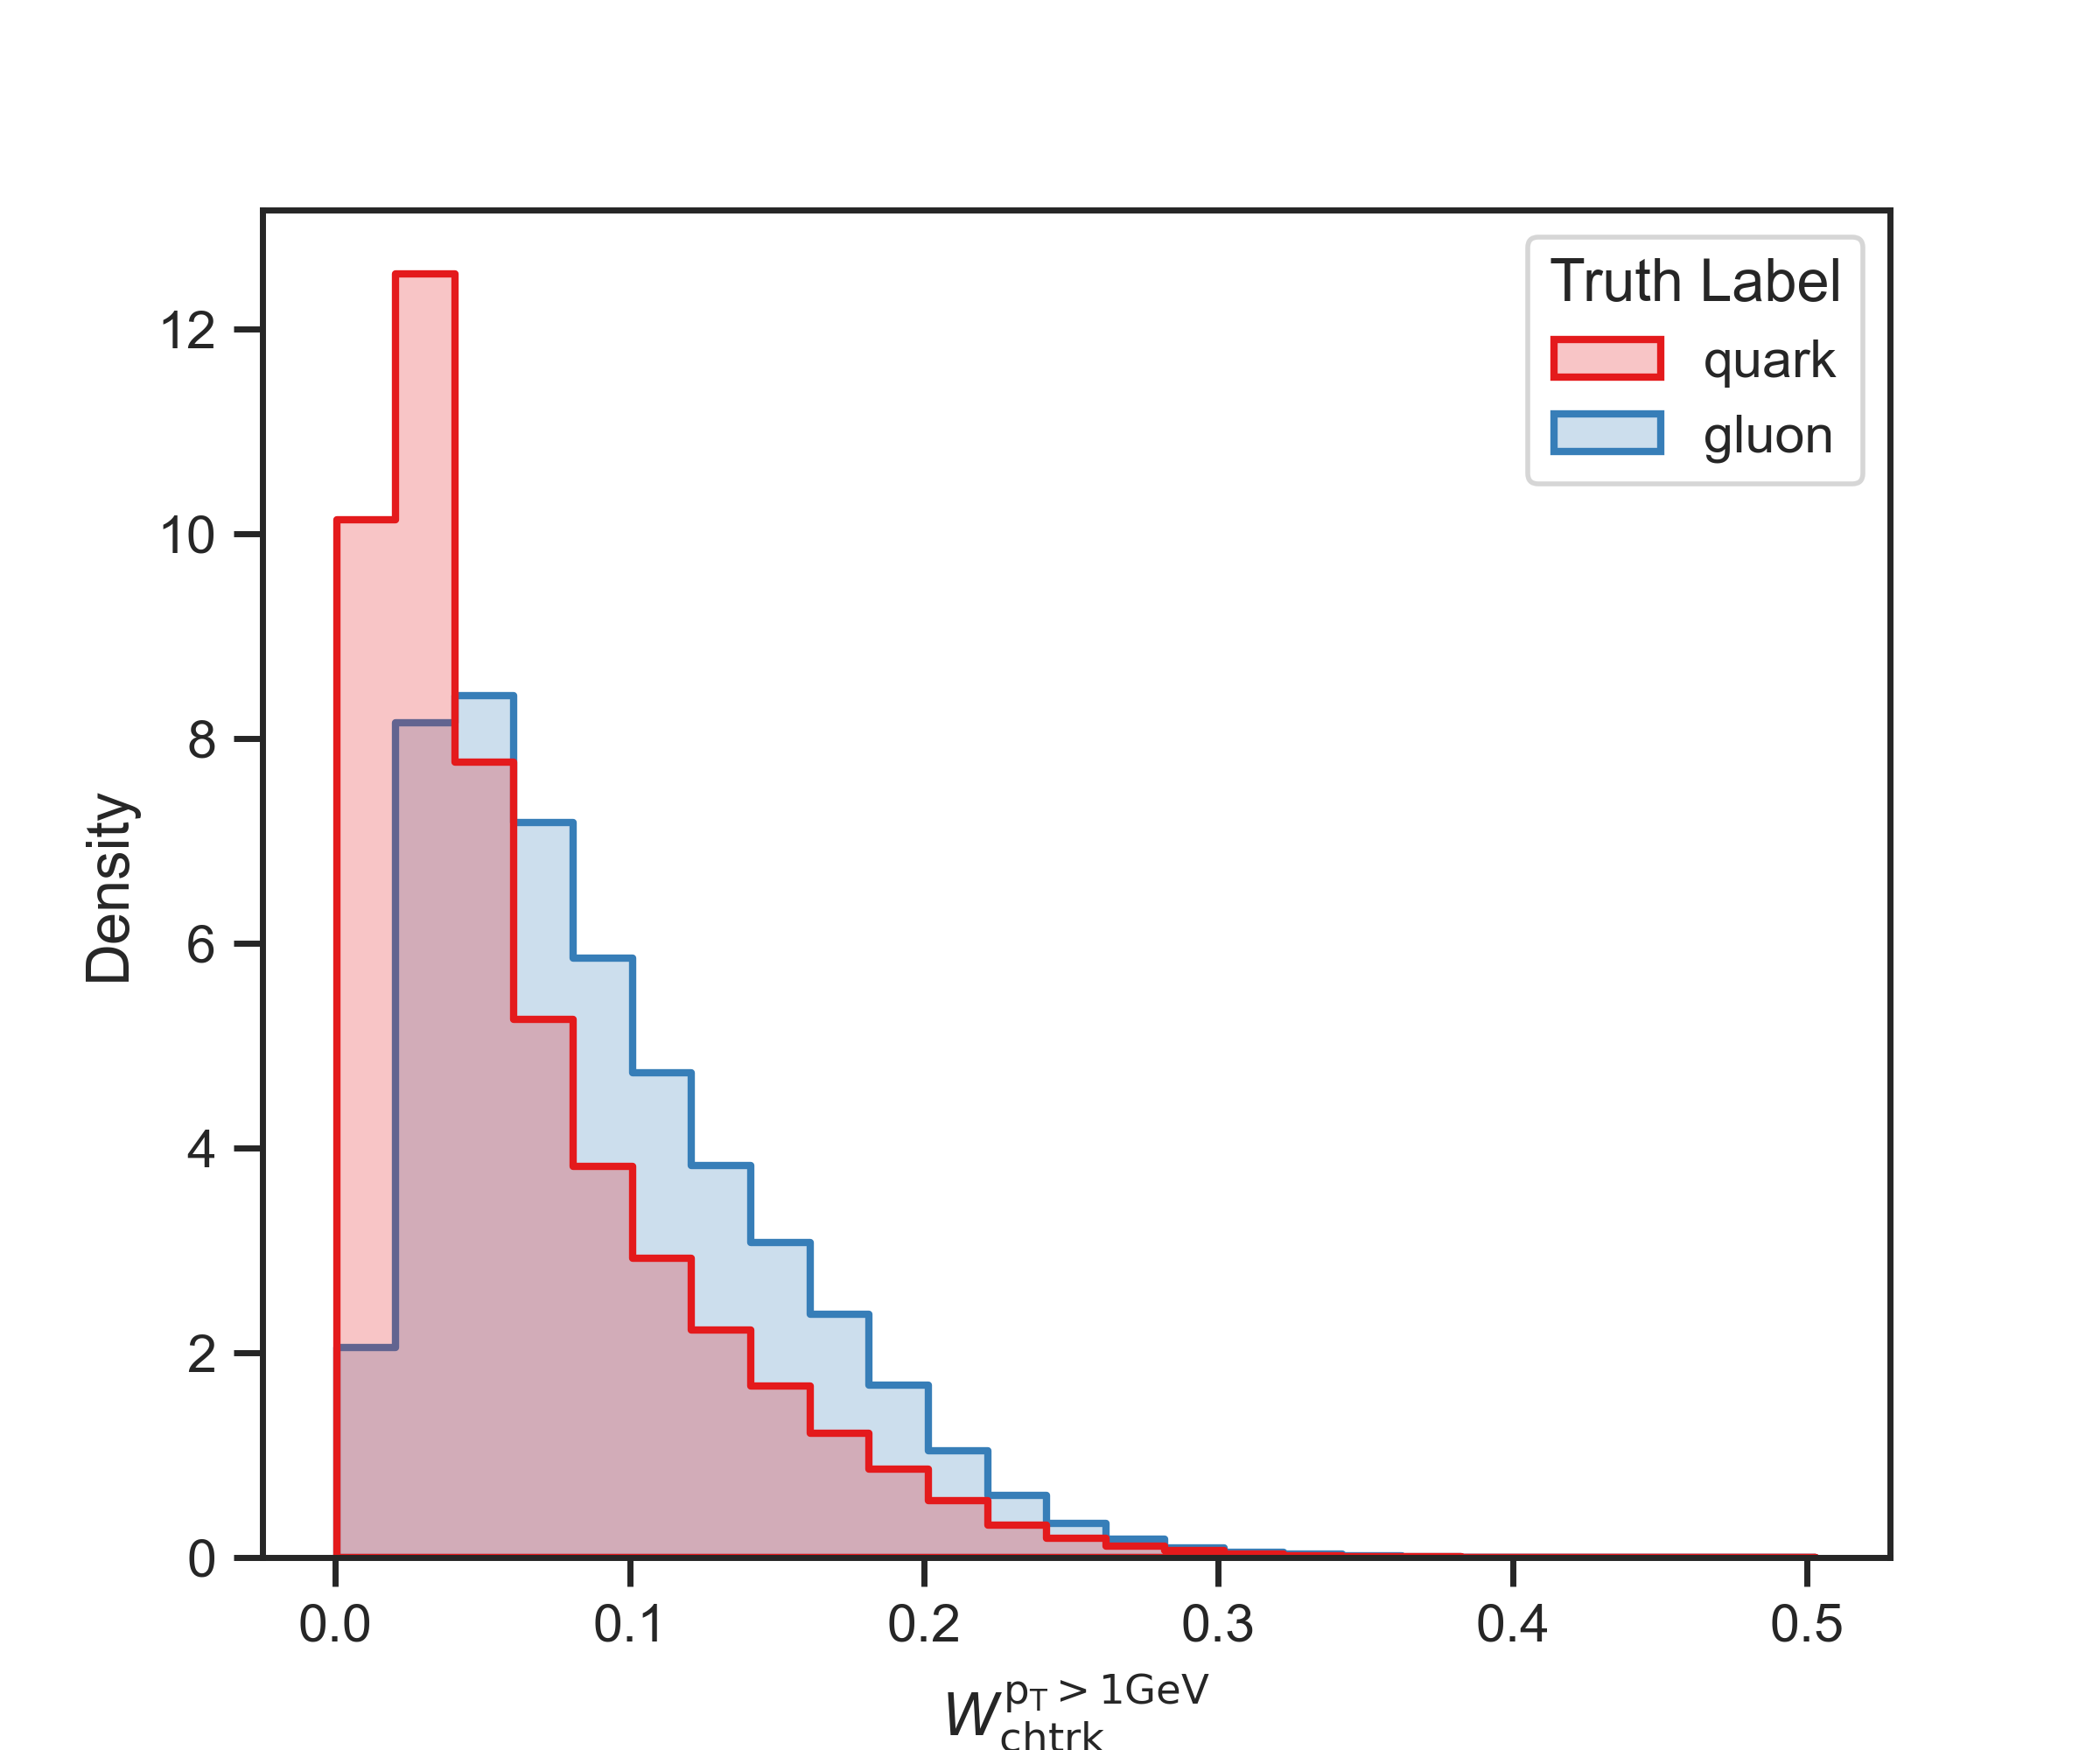
\includegraphics[width=1\textwidth]{src/plots/distributions/highlevel/jets_TrackWidthPt1000[0].png}
		\caption{\texttt{jets\_TrackWidthPt1000[0]}}
		\label{fig:highlevel_20}
	\end{subfigure}
	\begin{subfigure}[t]{0.48\textwidth}
		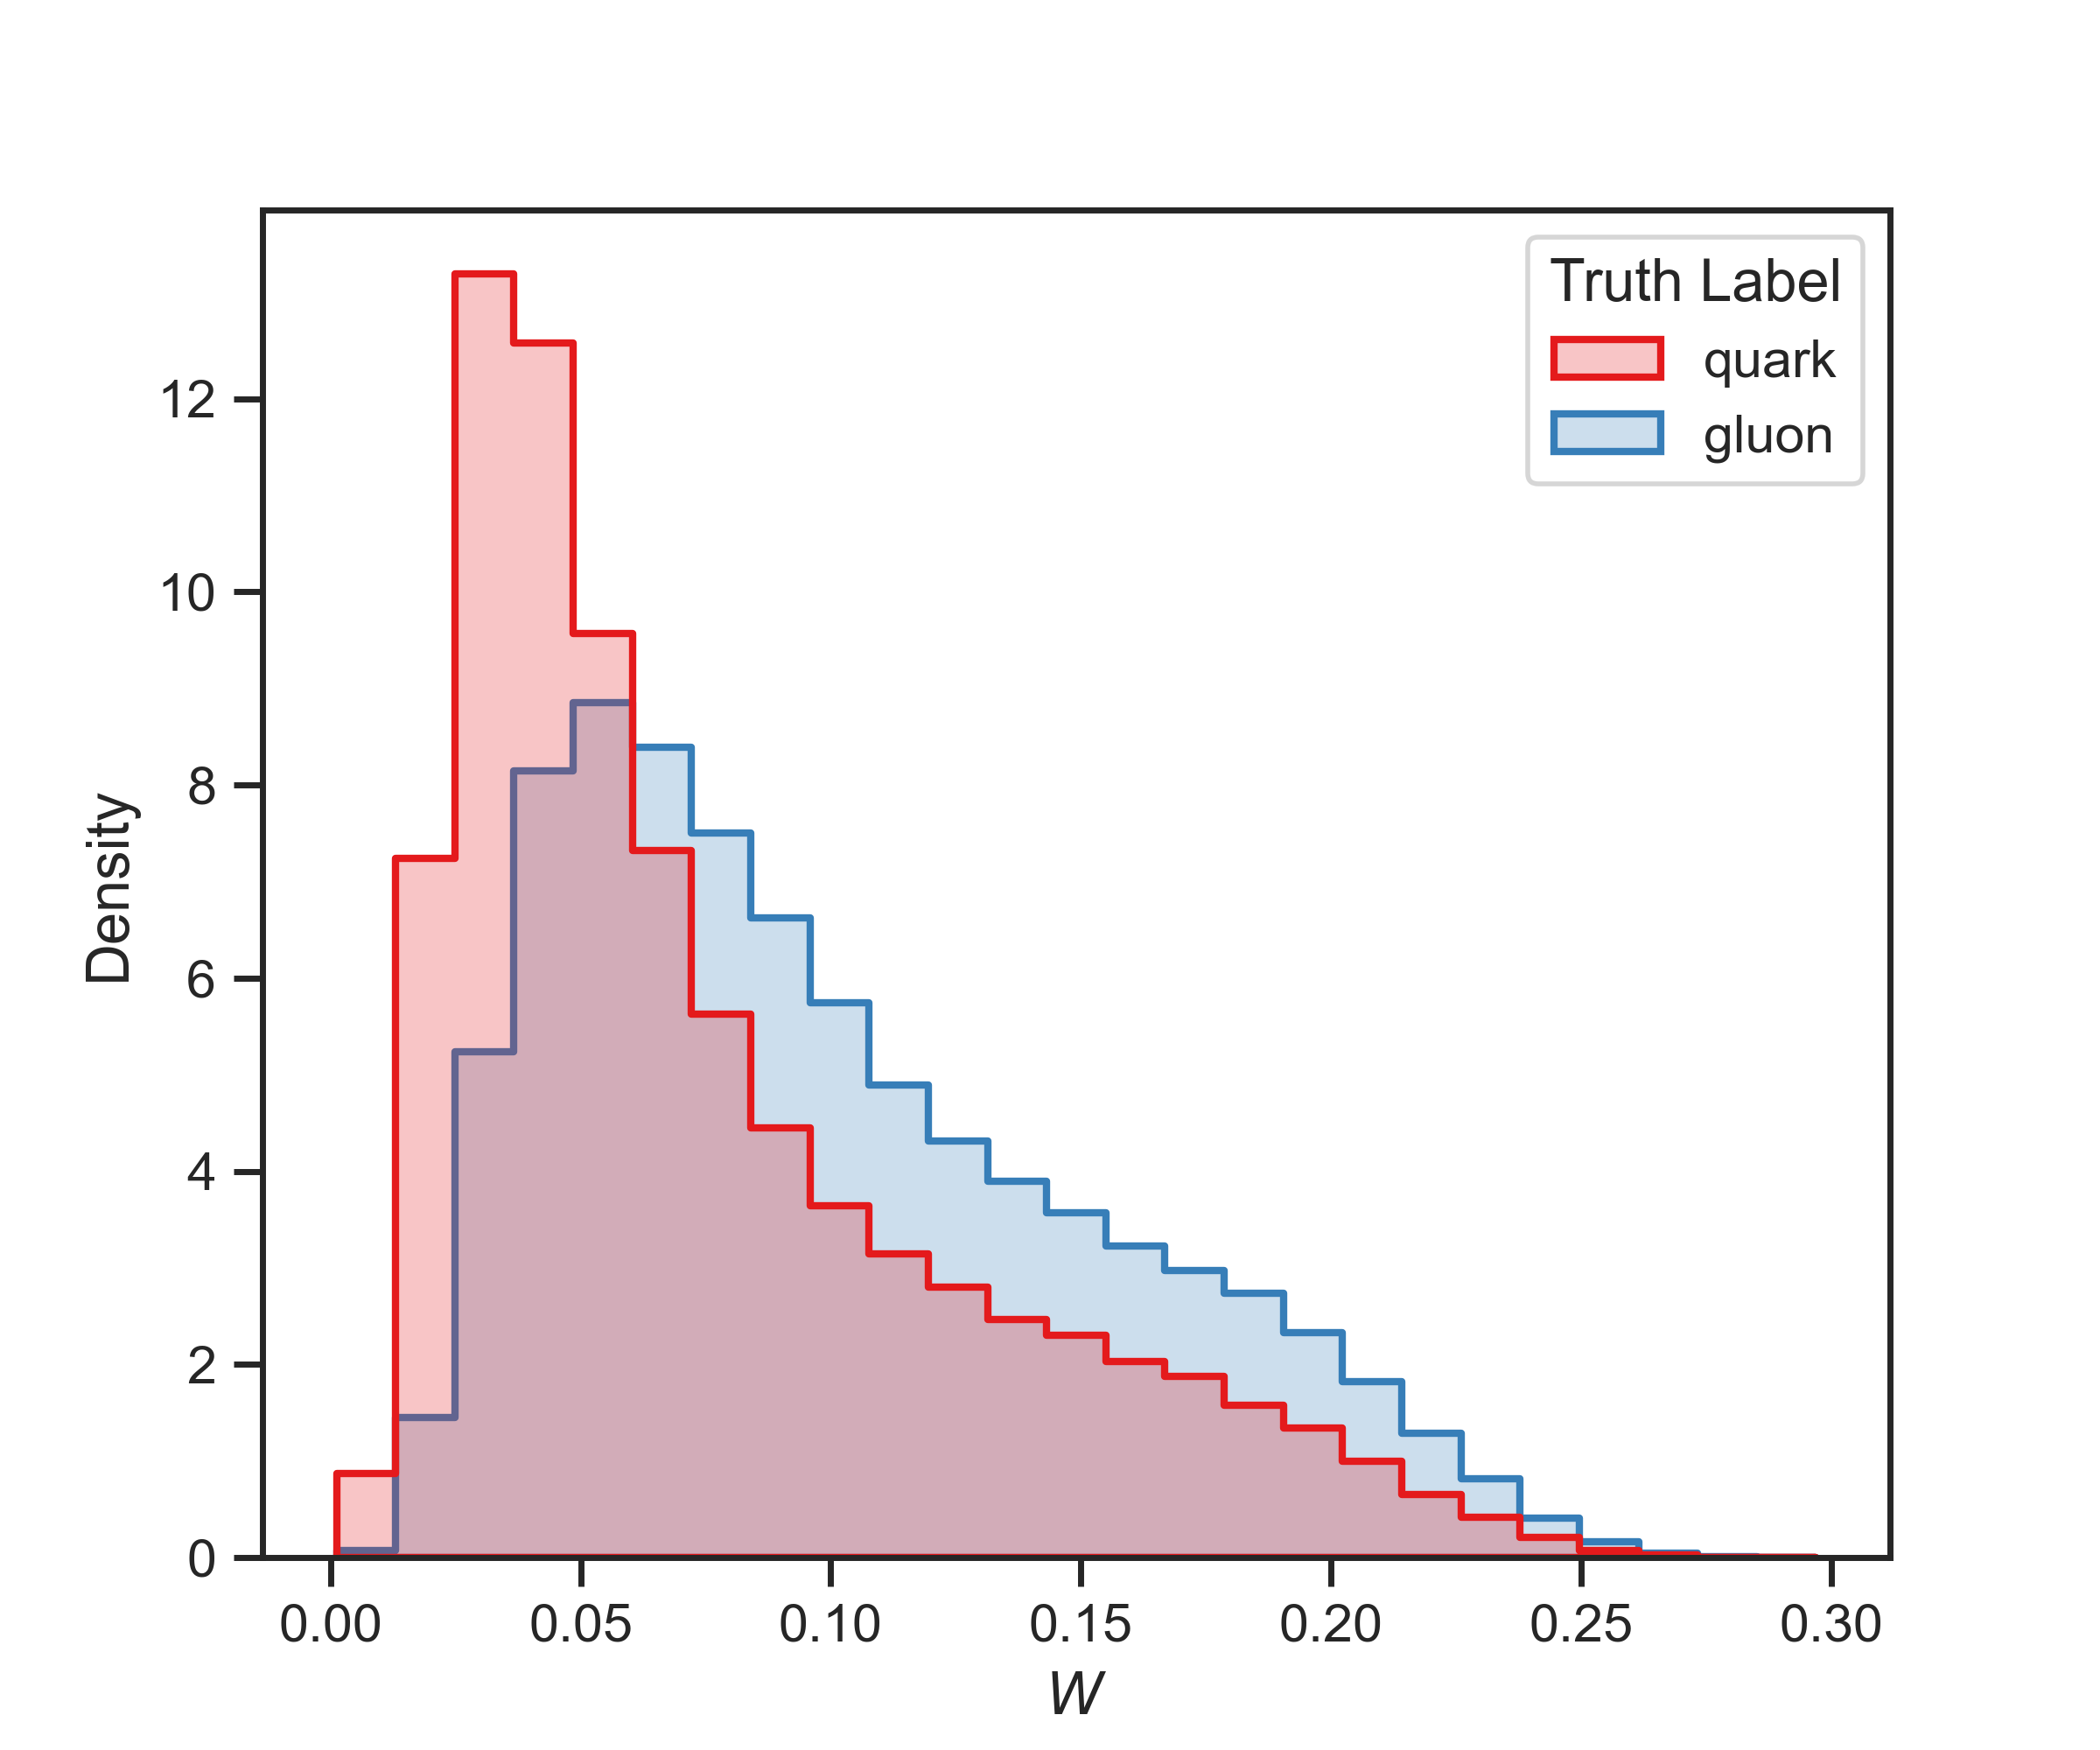
\includegraphics[width=1\textwidth]{src/plots/distributions/highlevel/jets_Width.png}
		\caption{\texttt{jets\_Width}}
		\label{fig:highlevel_21}
	\end{subfigure}
	\begin{subfigure}[t]{0.48\textwidth}
		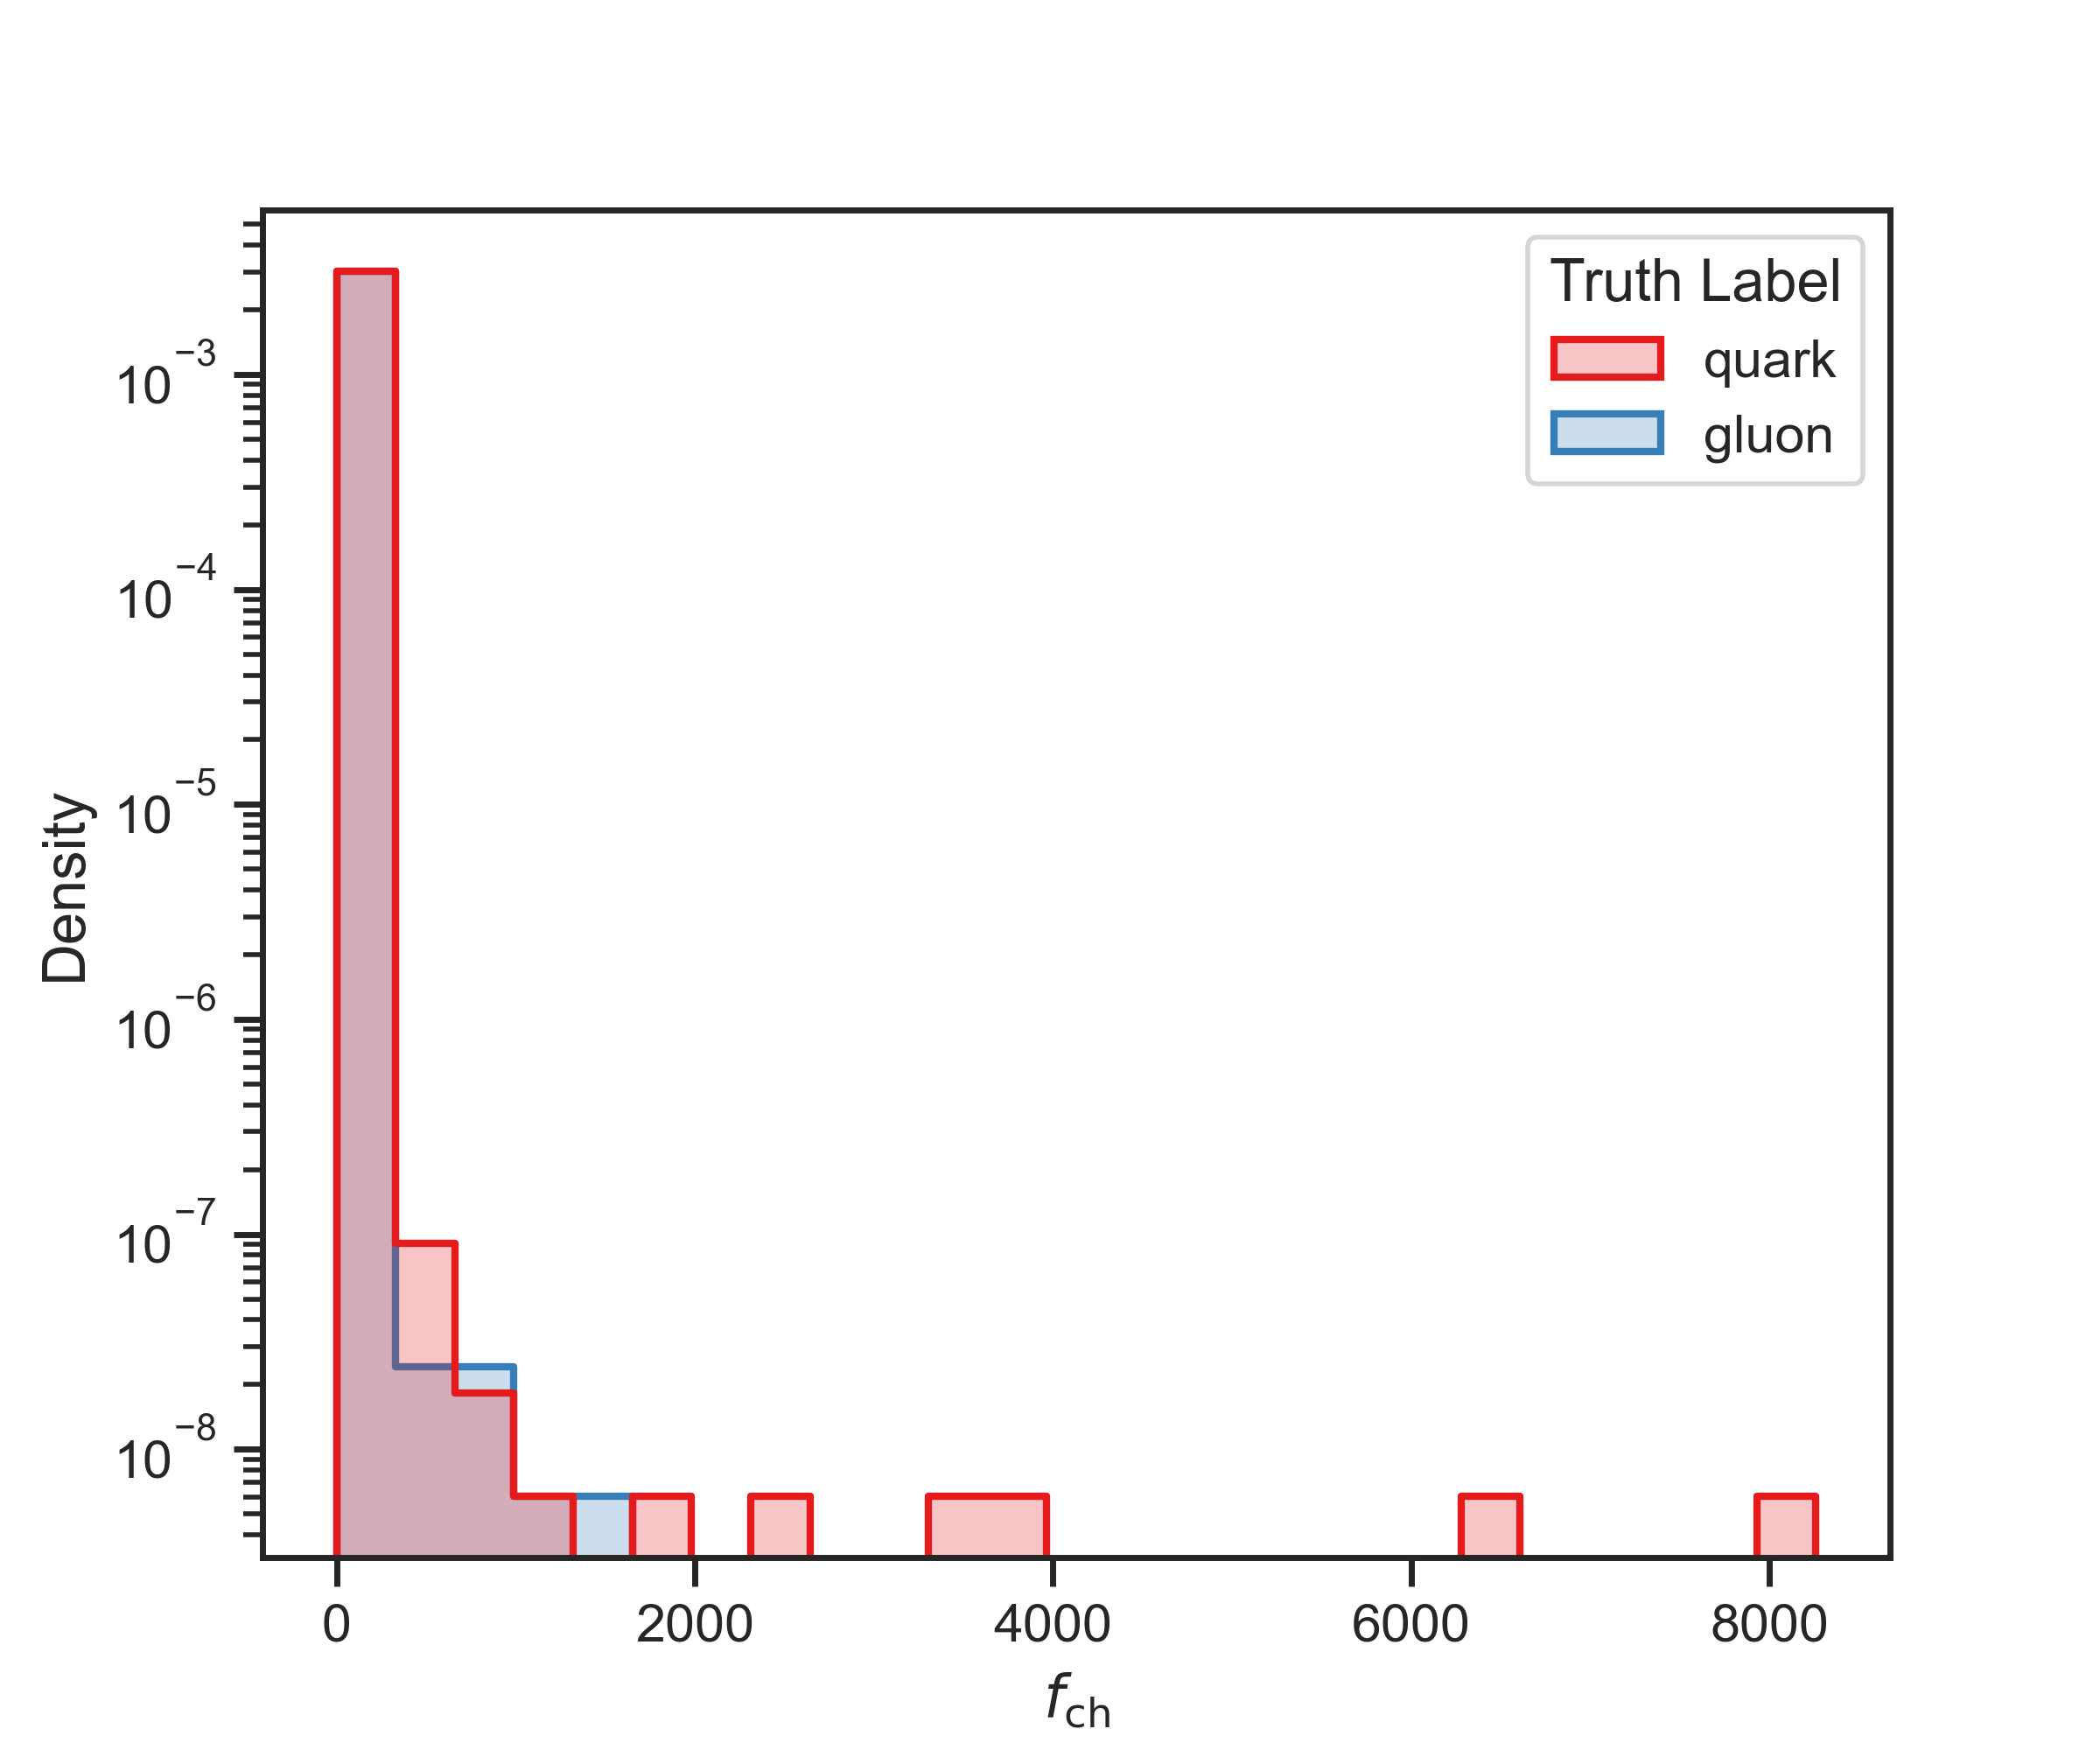
\includegraphics[width=1\textwidth]{src/plots/distributions/highlevel/jets_chf.png}
		\caption{\texttt{jets\_chf}}
		\label{fig:highlevel_22}
	\end{subfigure}
	\begin{subfigure}[t]{0.48\textwidth}
		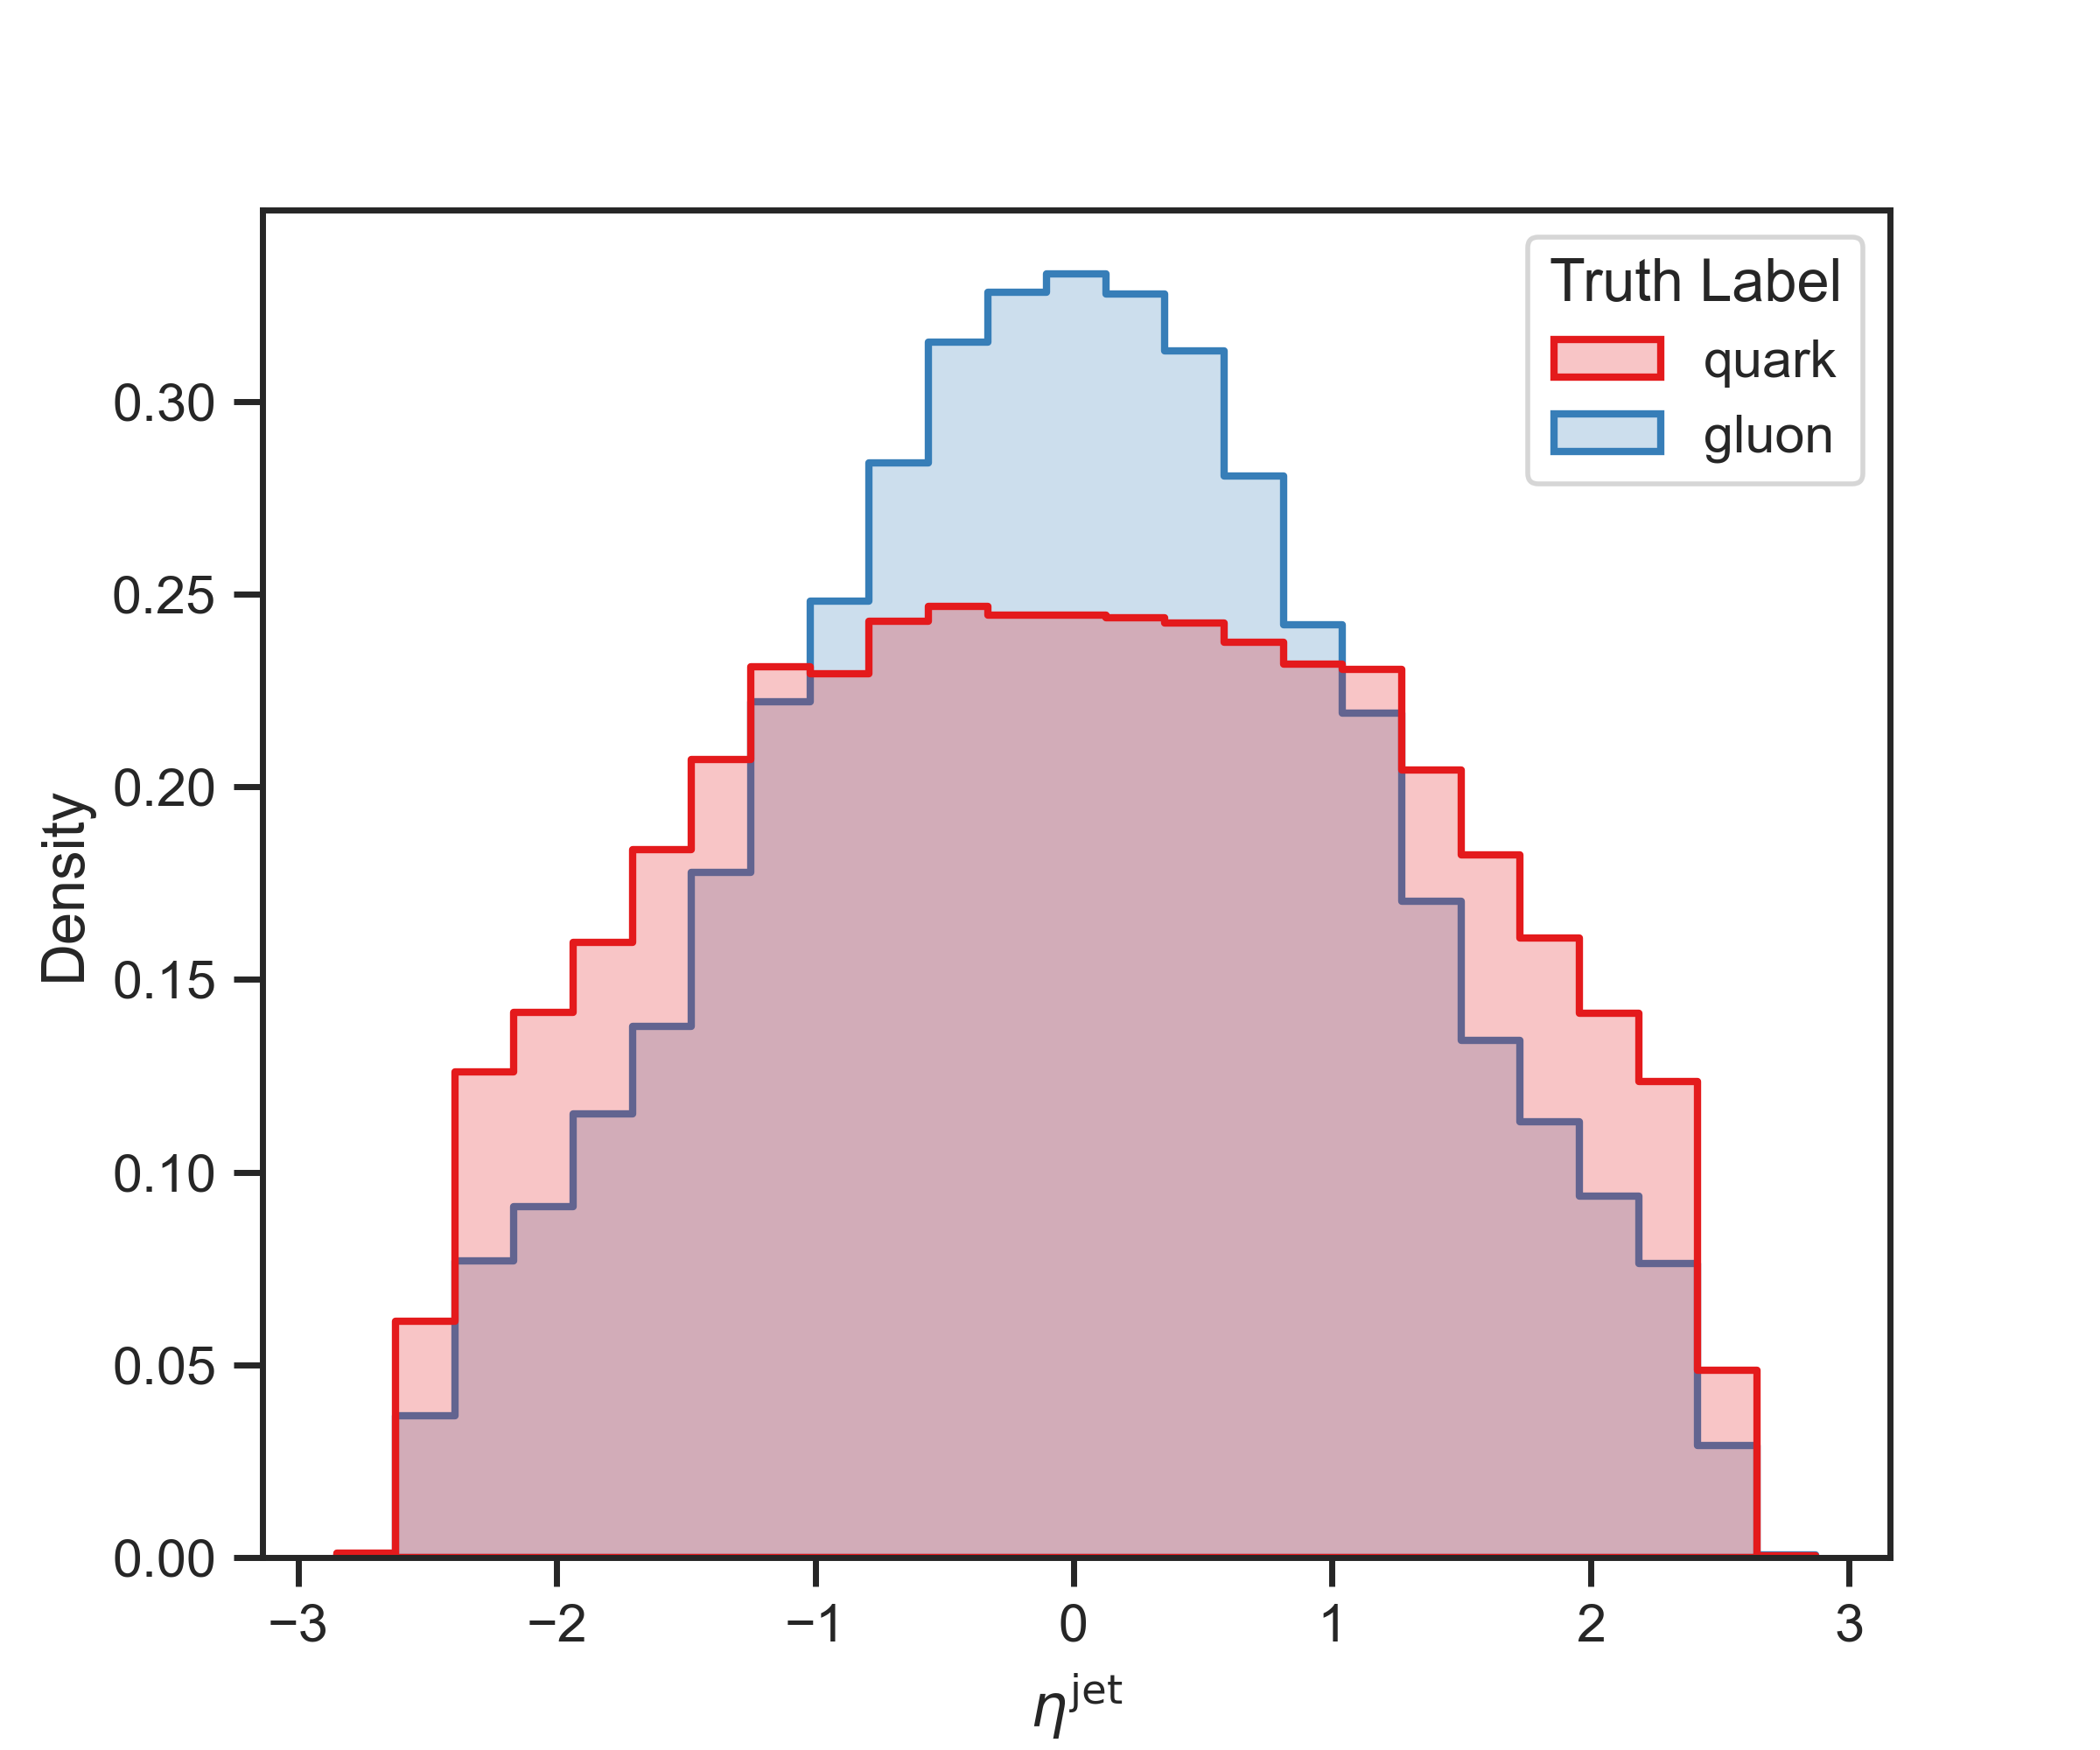
\includegraphics[width=1\textwidth]{src/plots/distributions/highlevel/jets_eta.png}
		\caption{\texttt{jets\_eta}}
		\label{fig:highlevel_23}
	\end{subfigure}
\caption{High-level Jet Variables, part 4}
\label{fig:highlevel_18-23}
\end{figure}

\begin{figure}[!htb]
	\centering
	\begin{subfigure}[t]{0.48\textwidth}
		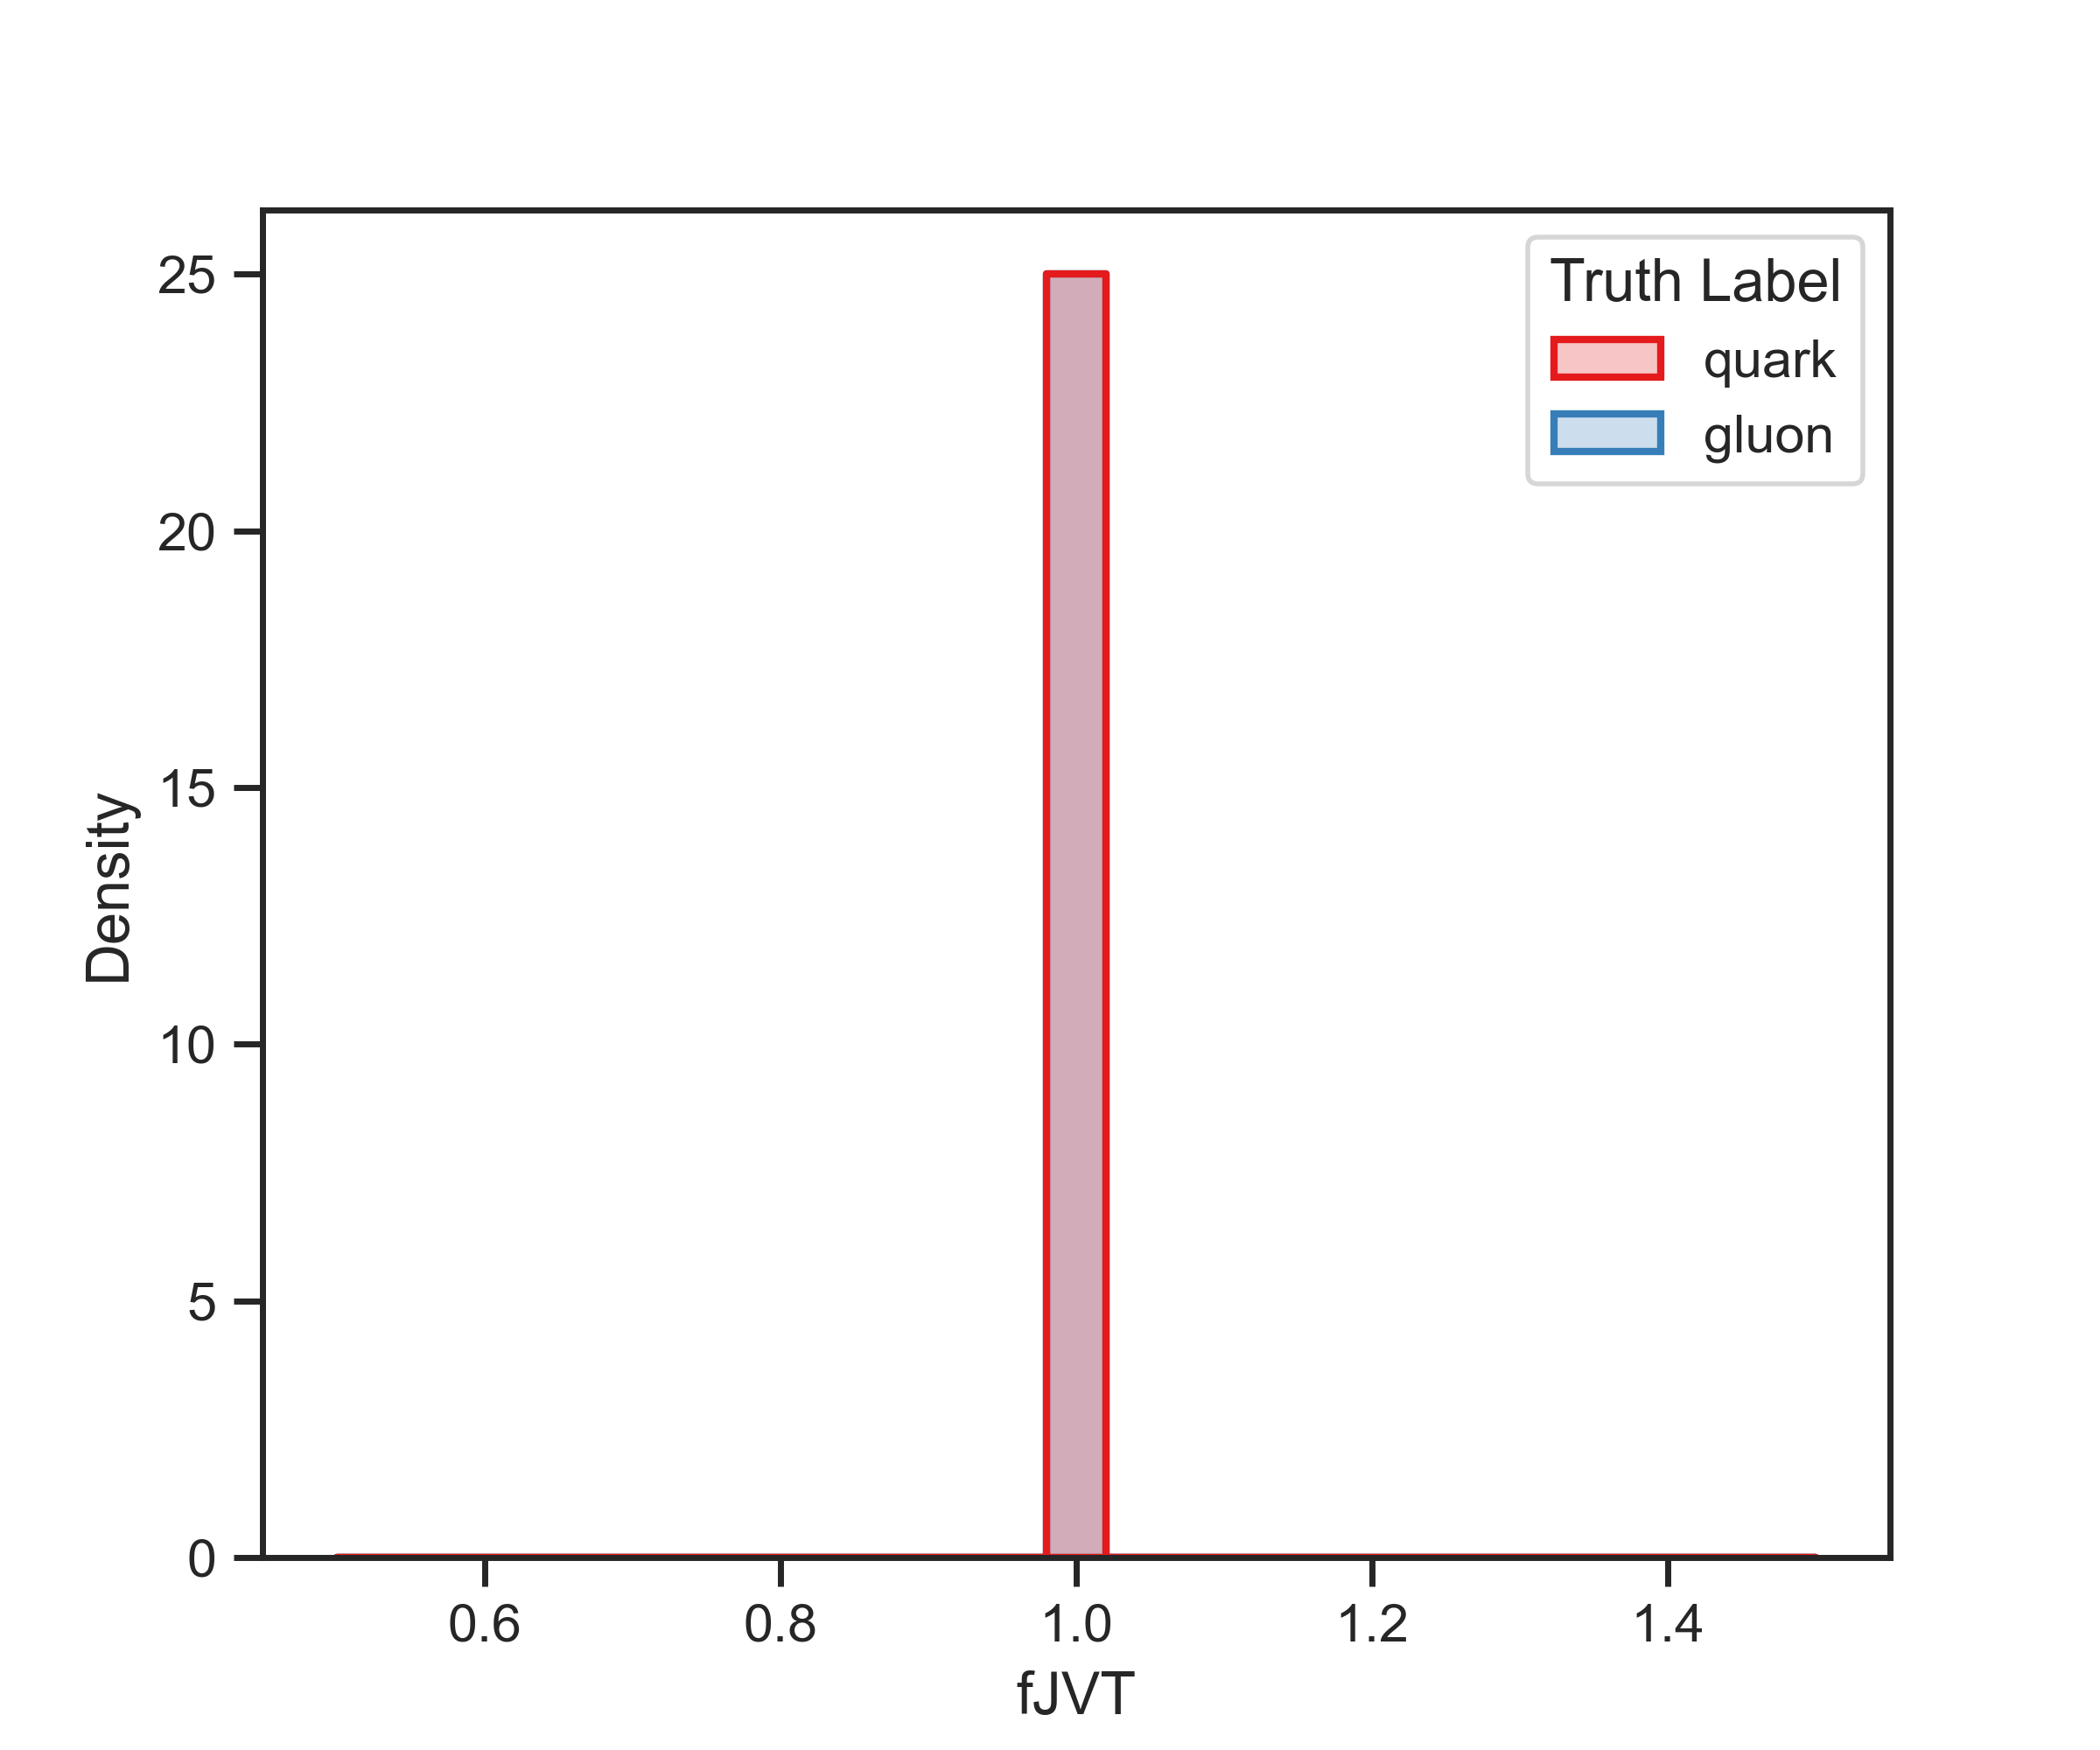
\includegraphics[width=1\textwidth]{src/plots/distributions/highlevel/jets_fJVT.png}
		\caption{\texttt{jets\_fJVT}}
		\label{fig:highlevel_24}
	\end{subfigure}
	\begin{subfigure}[t]{0.48\textwidth}
		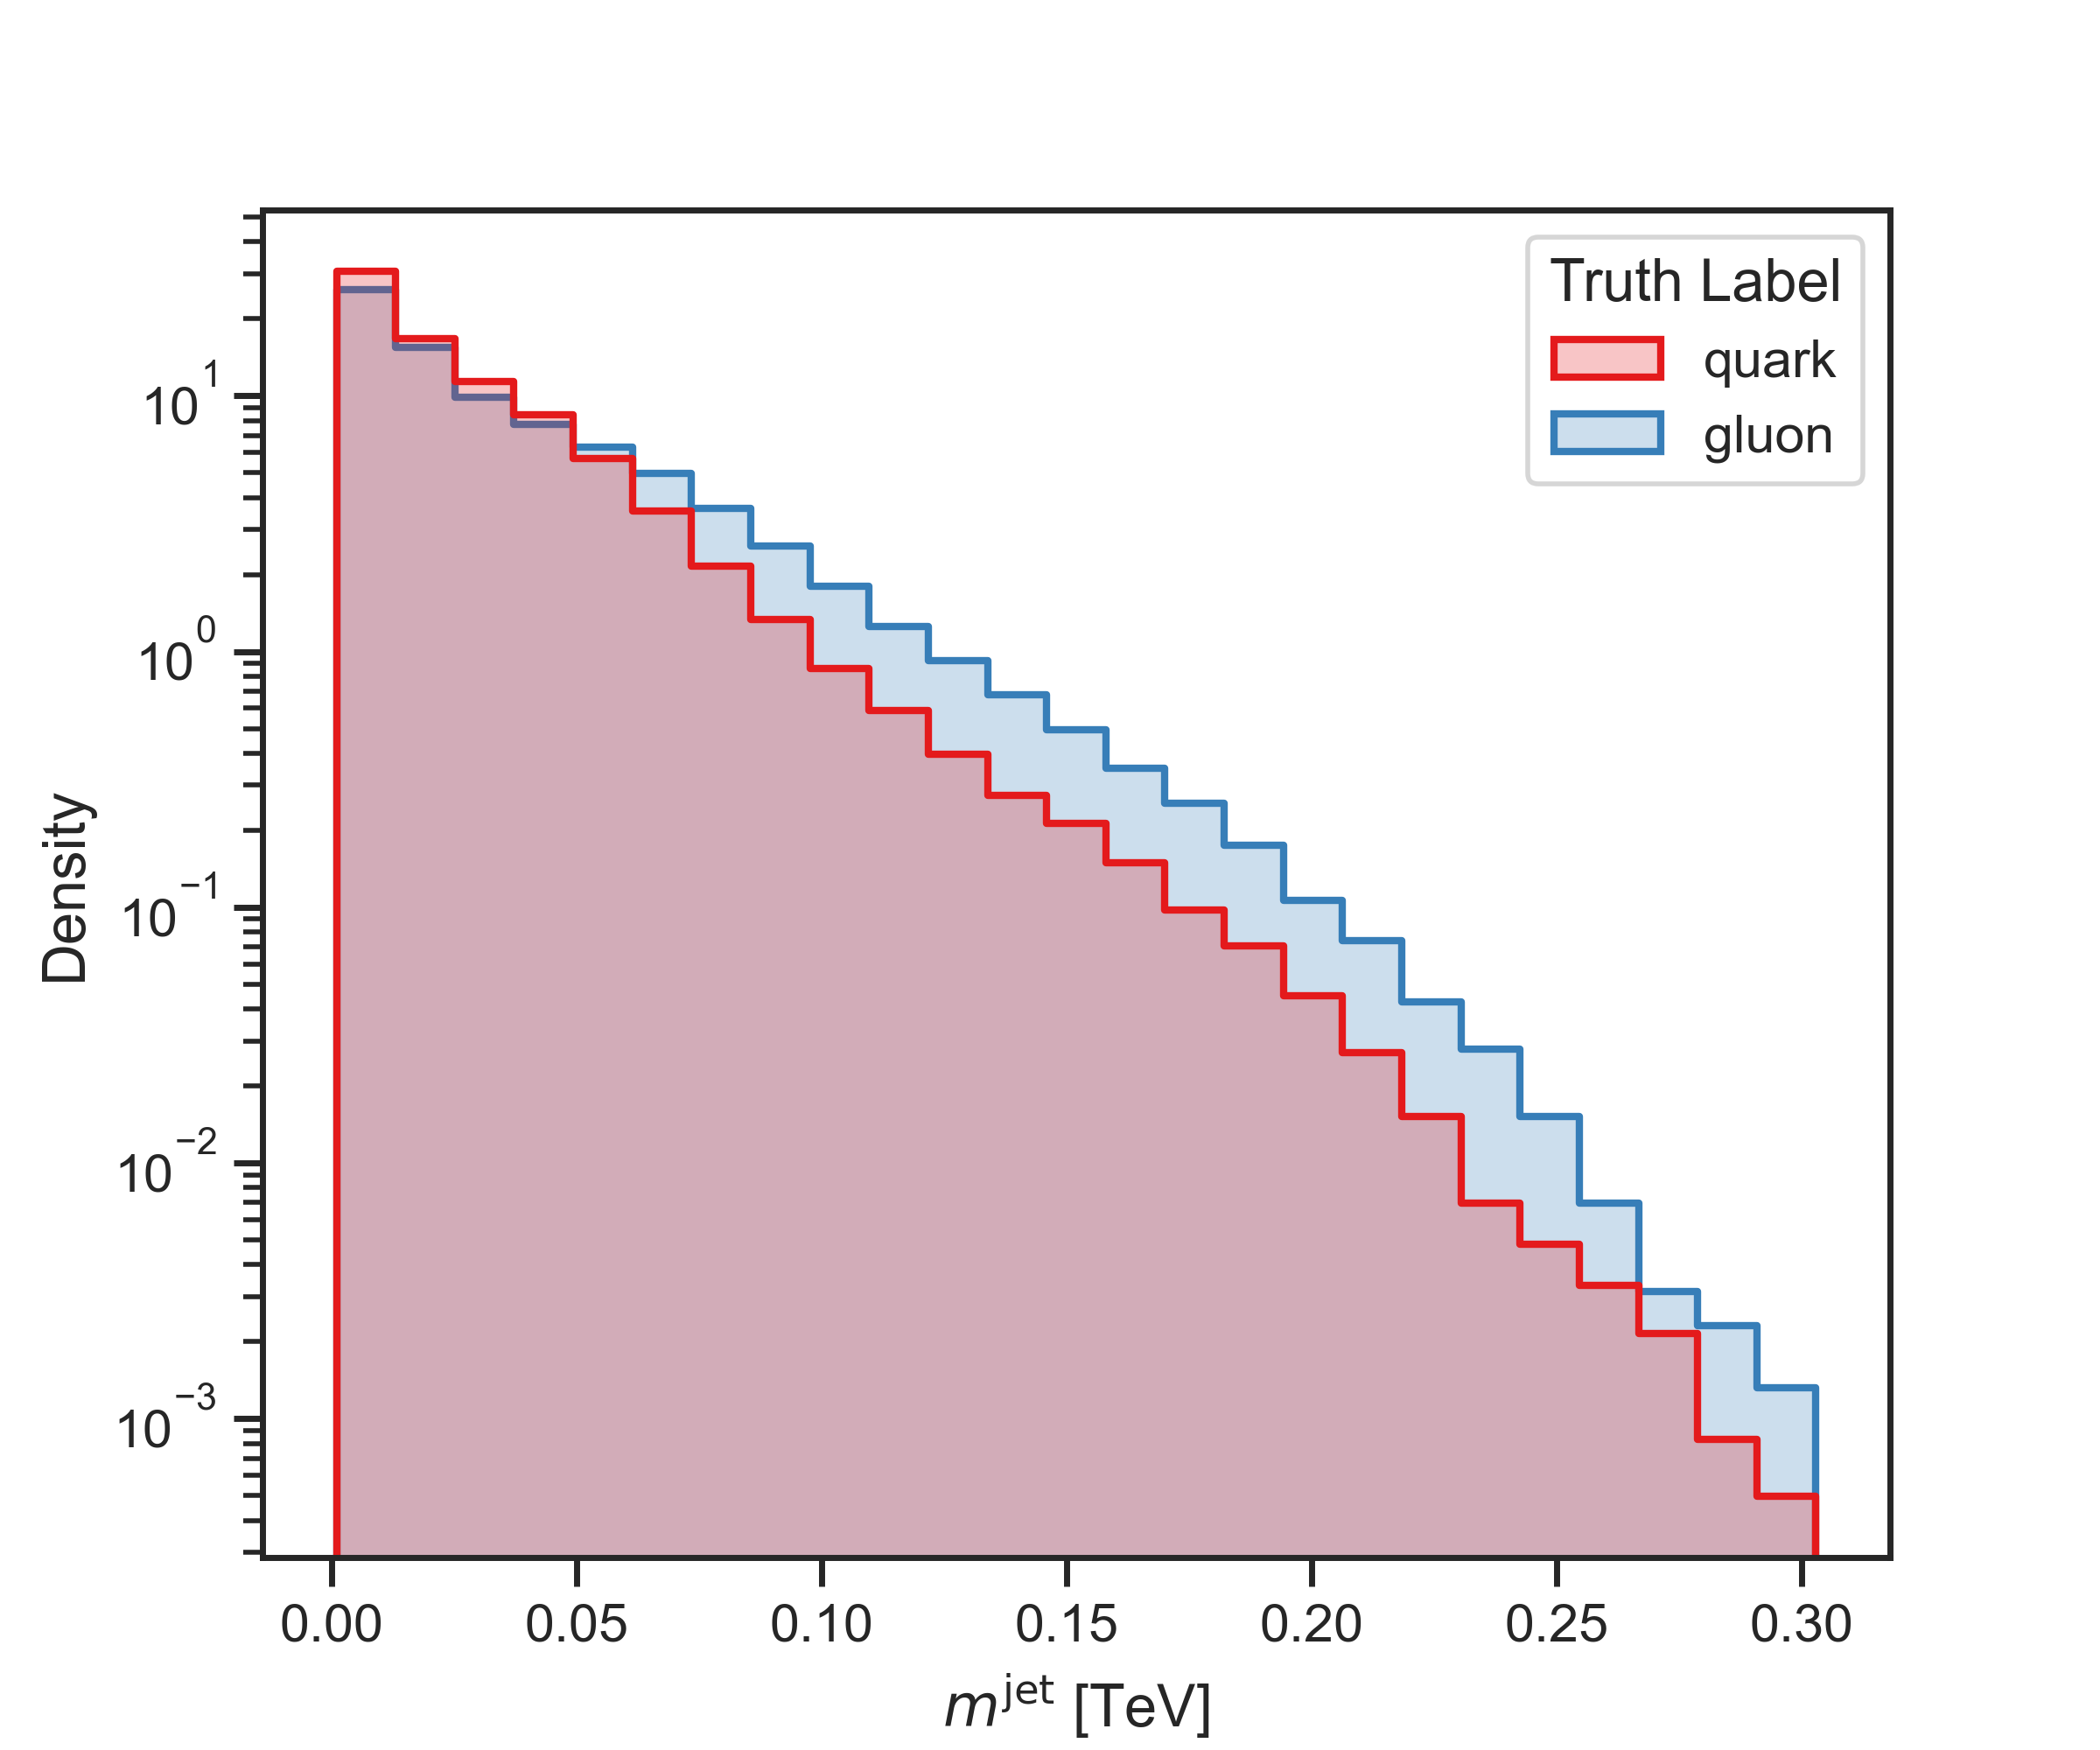
\includegraphics[width=1\textwidth]{src/plots/distributions/highlevel/jets_m.png}
		\caption{\texttt{jets\_m}}
		\label{fig:highlevel_25}
	\end{subfigure}
	\begin{subfigure}[t]{0.48\textwidth}
		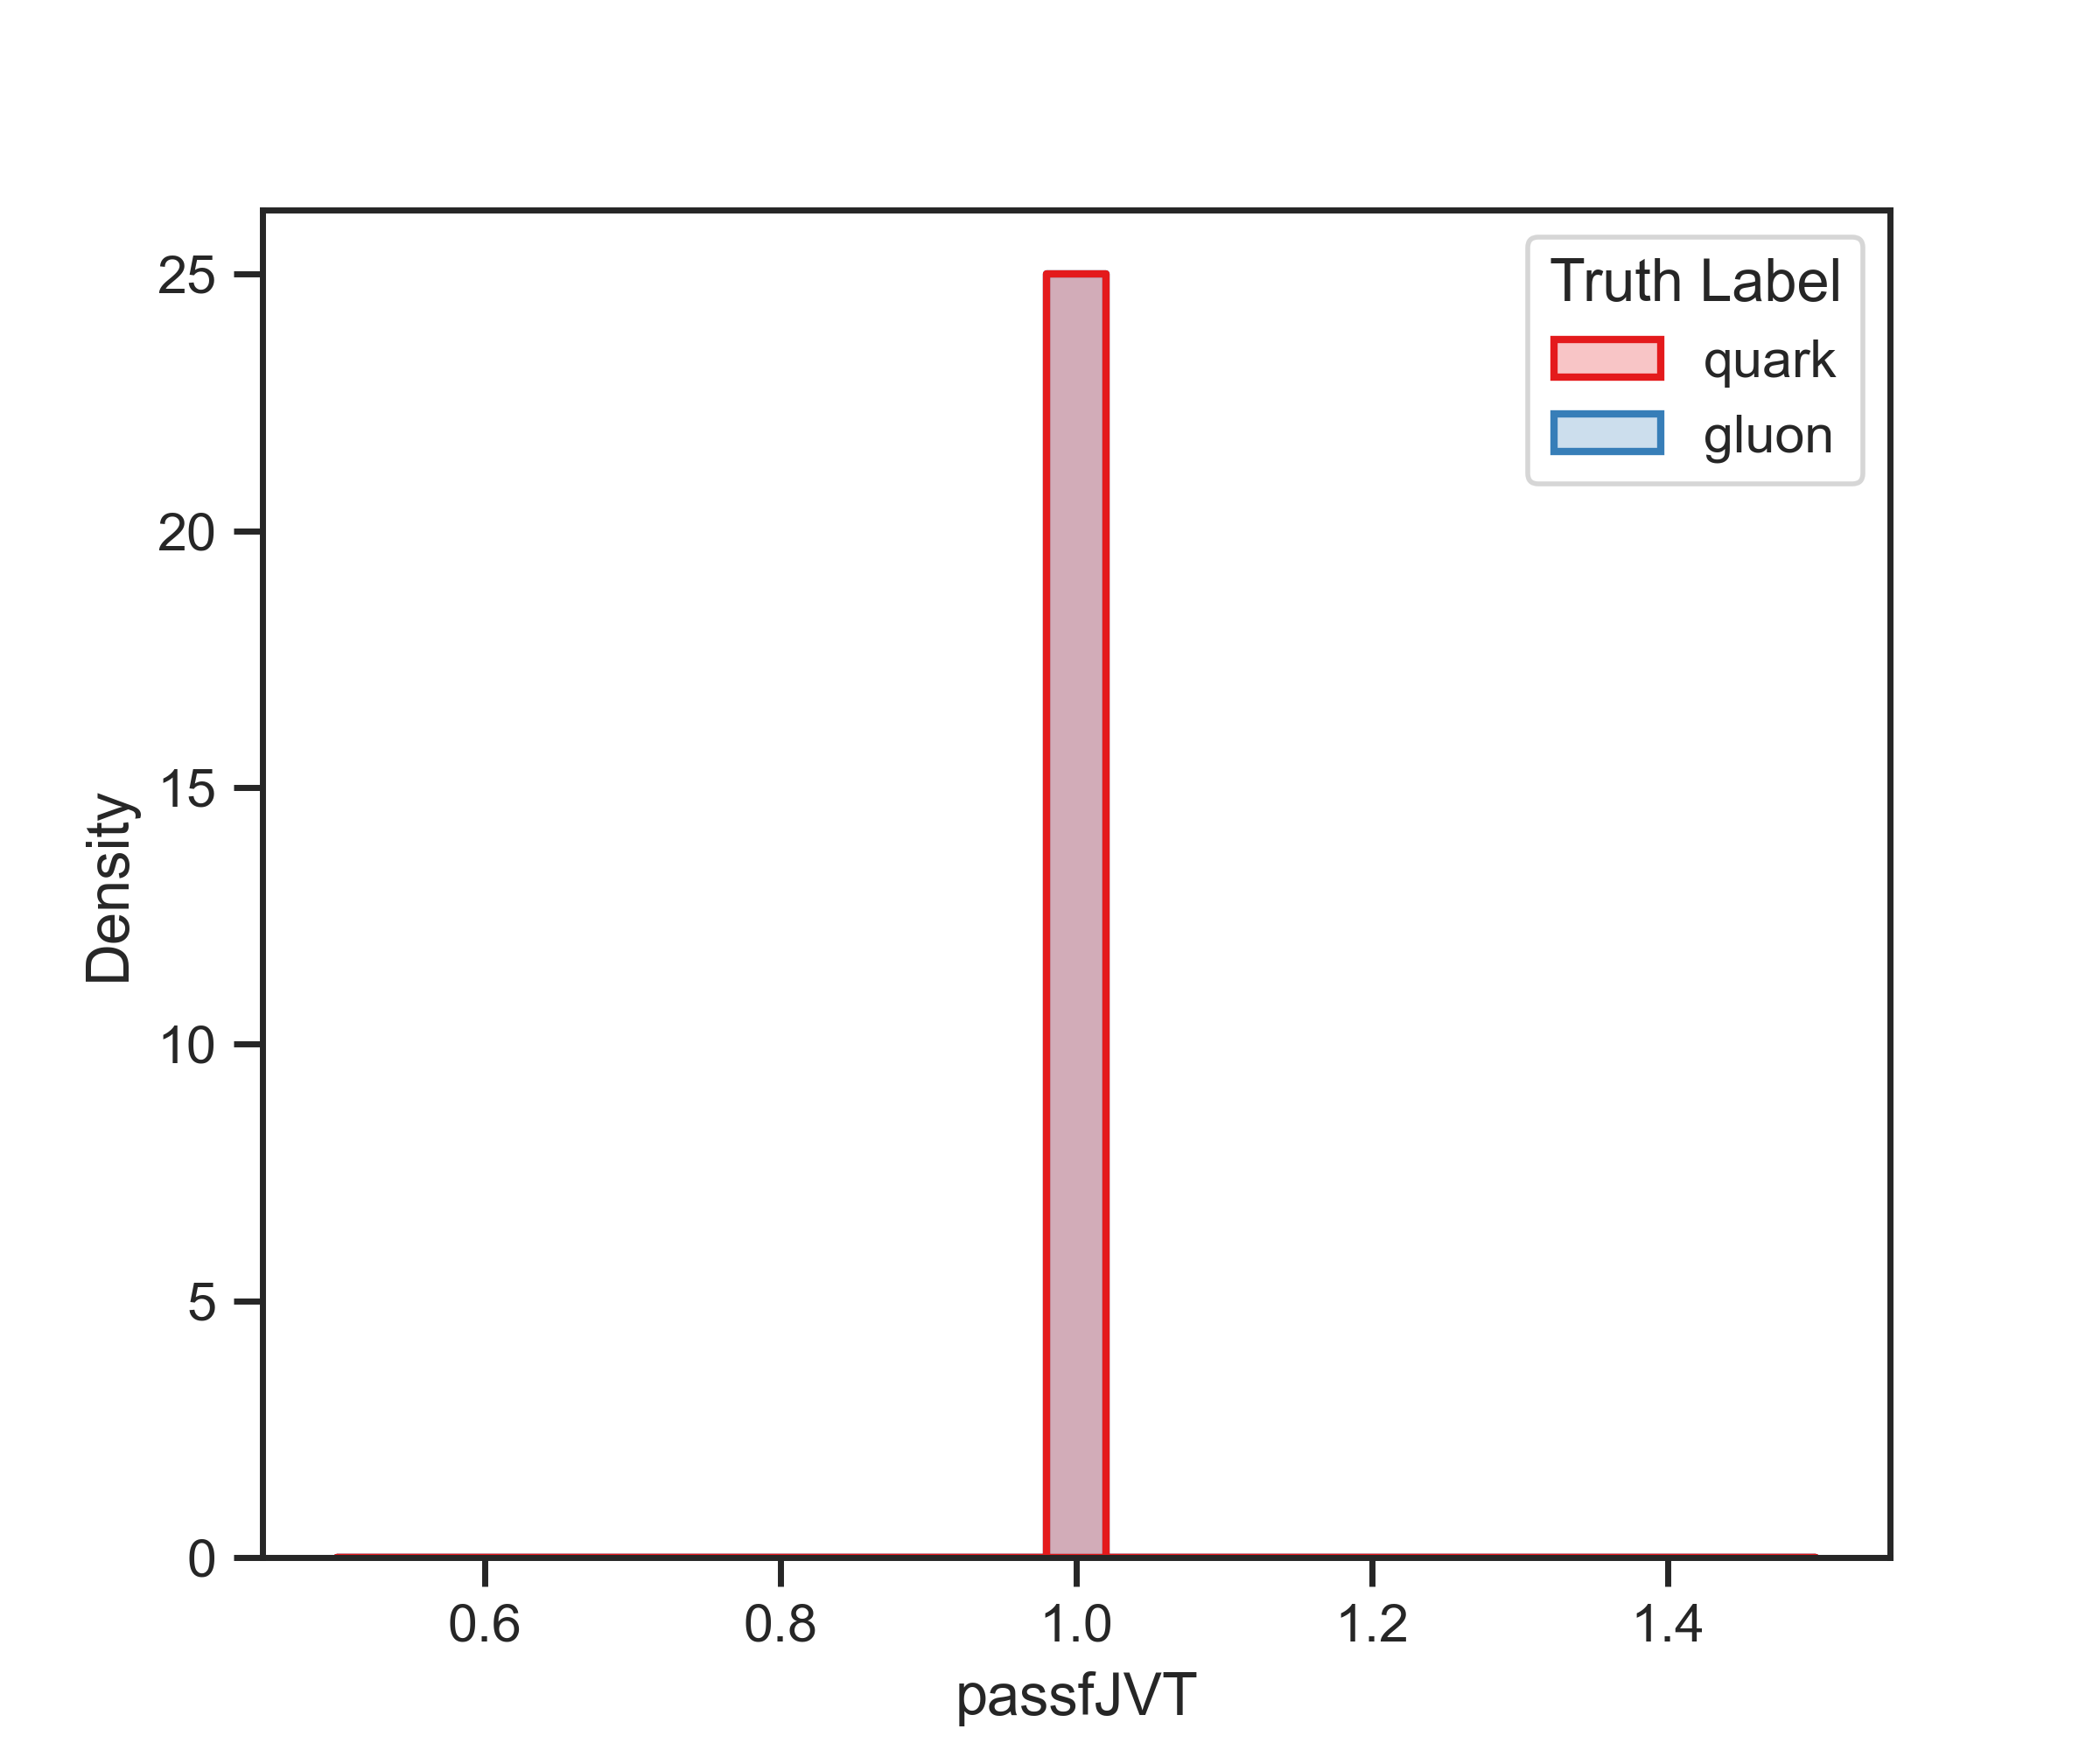
\includegraphics[width=1\textwidth]{src/plots/distributions/highlevel/jets_passFJVT.png}
		\caption{\texttt{jets\_passFJVT}}
		\label{fig:highlevel_26}
	\end{subfigure}
	\begin{subfigure}[t]{0.48\textwidth}
		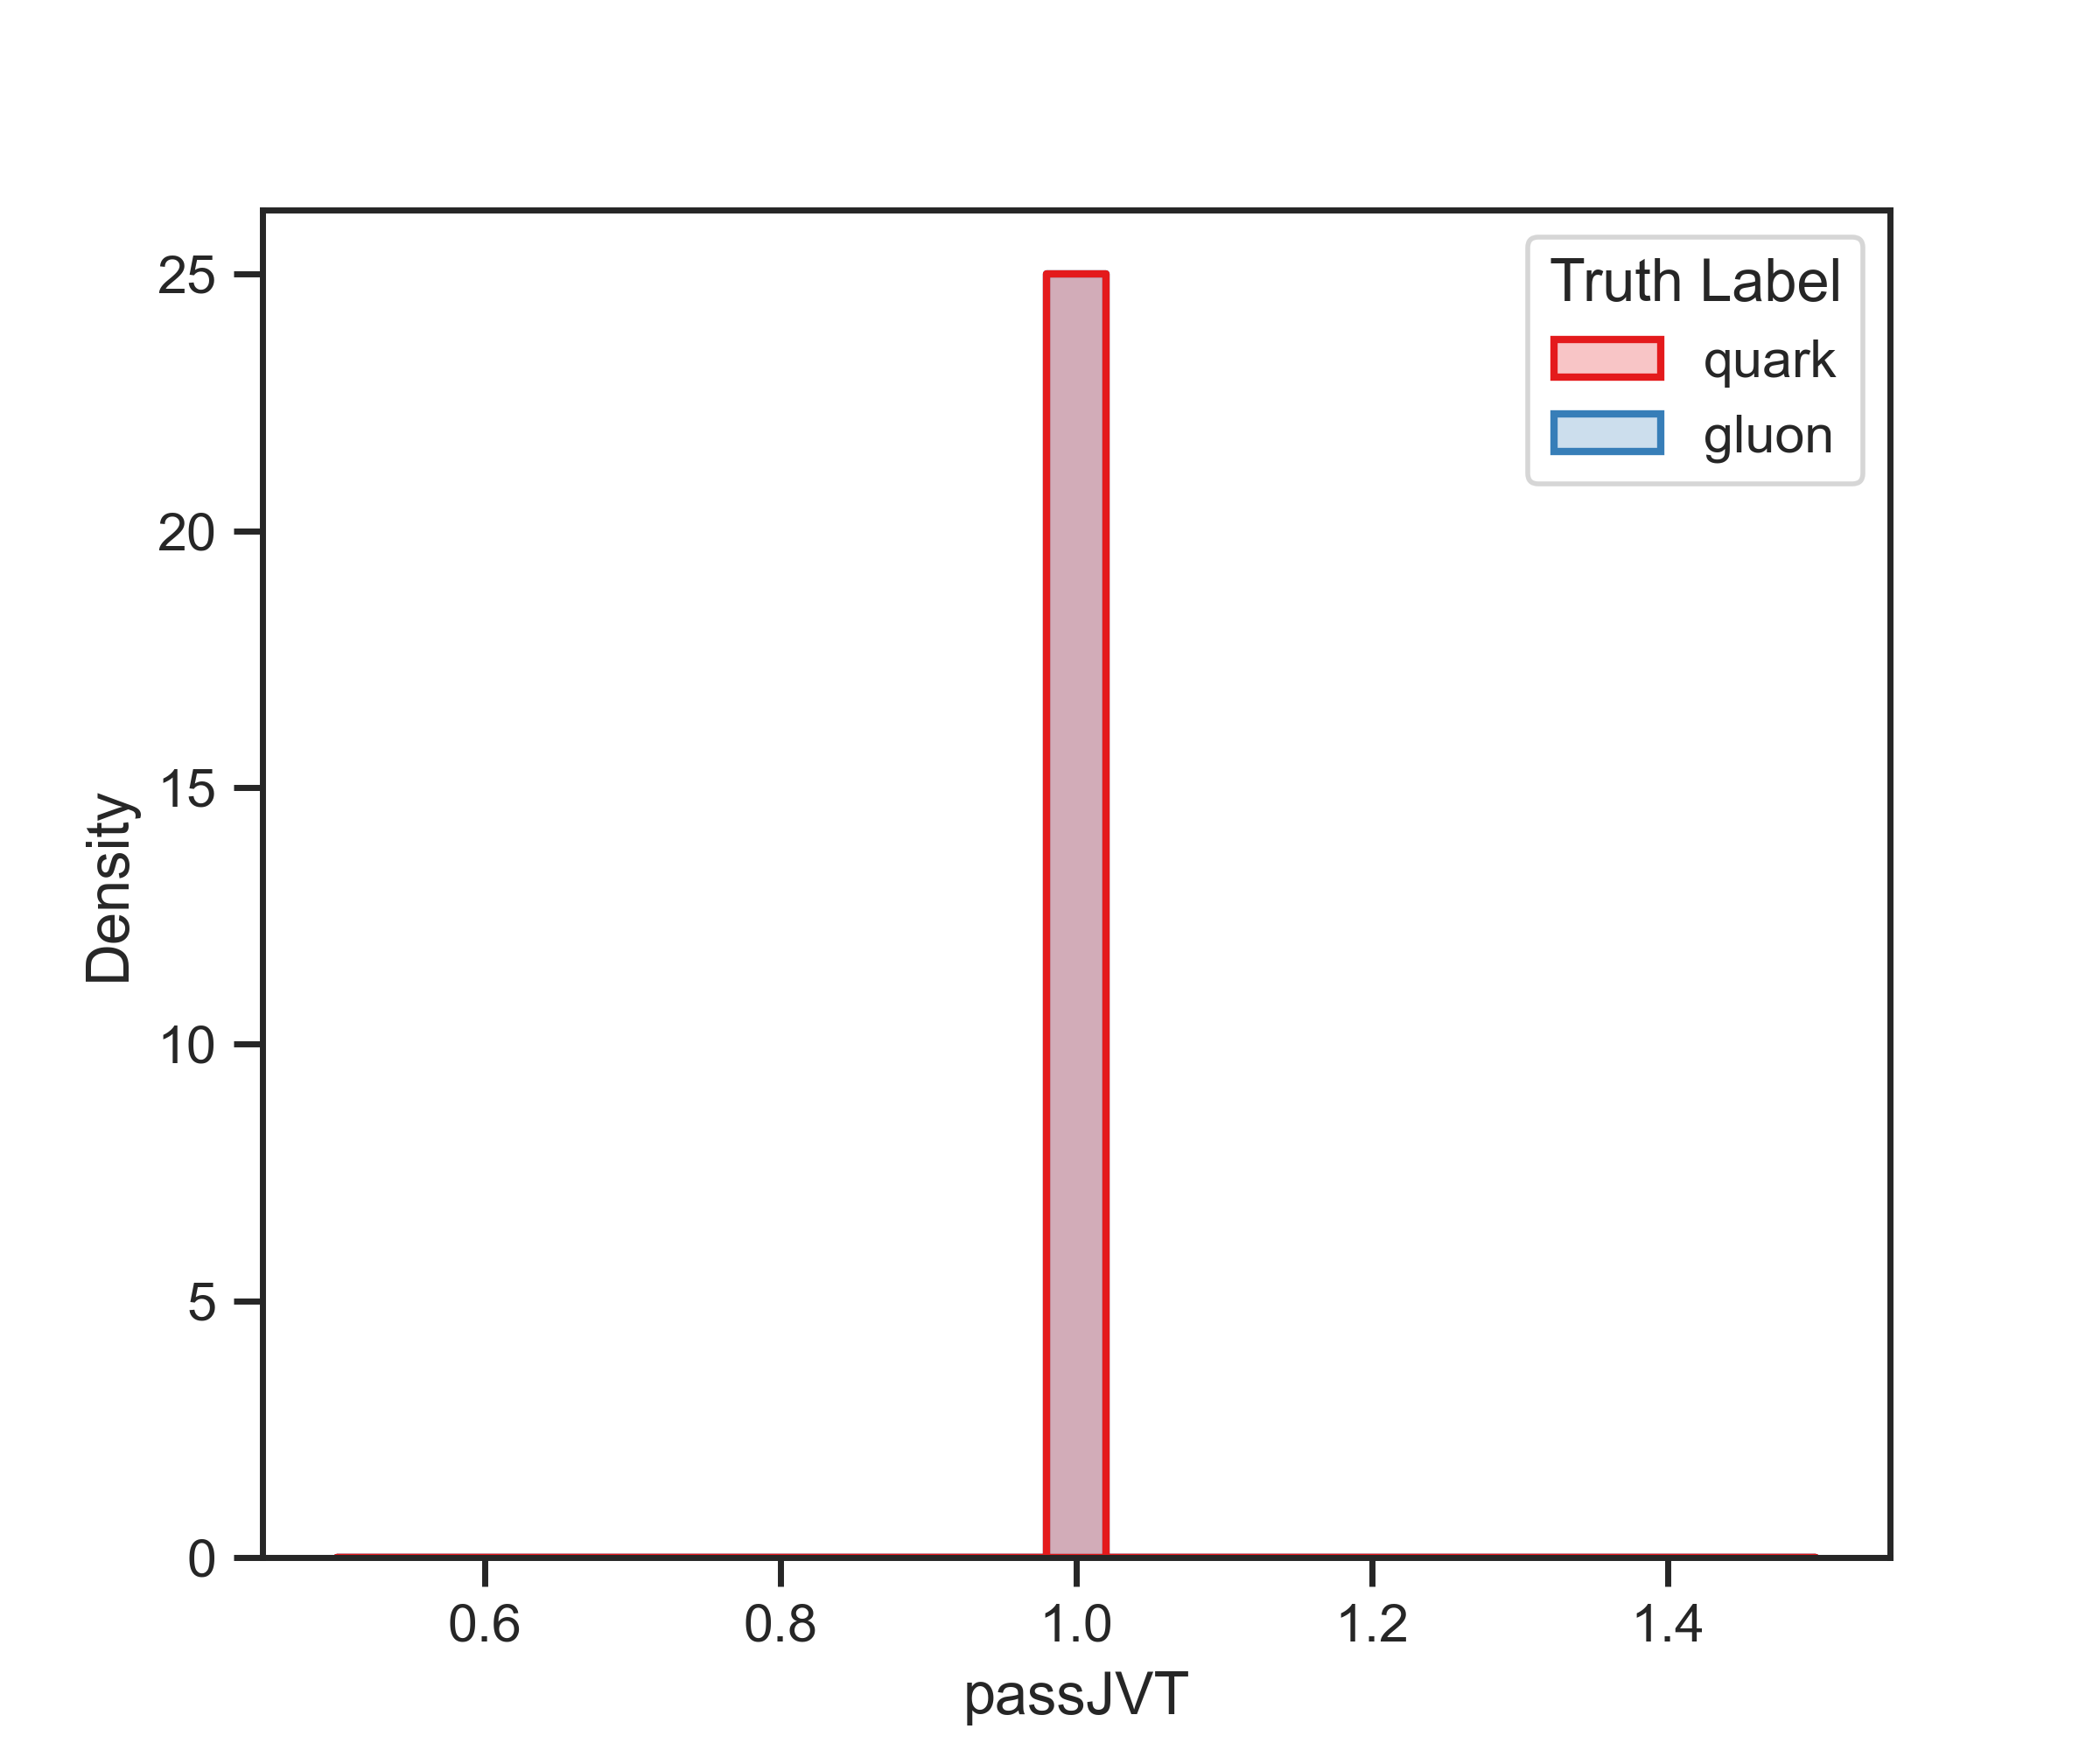
\includegraphics[width=1\textwidth]{src/plots/distributions/highlevel/jets_passJVT.png}
		\caption{\texttt{jets\_passJVT}}
		\label{fig:highlevel_27}
	\end{subfigure}
	\begin{subfigure}[t]{0.48\textwidth}
		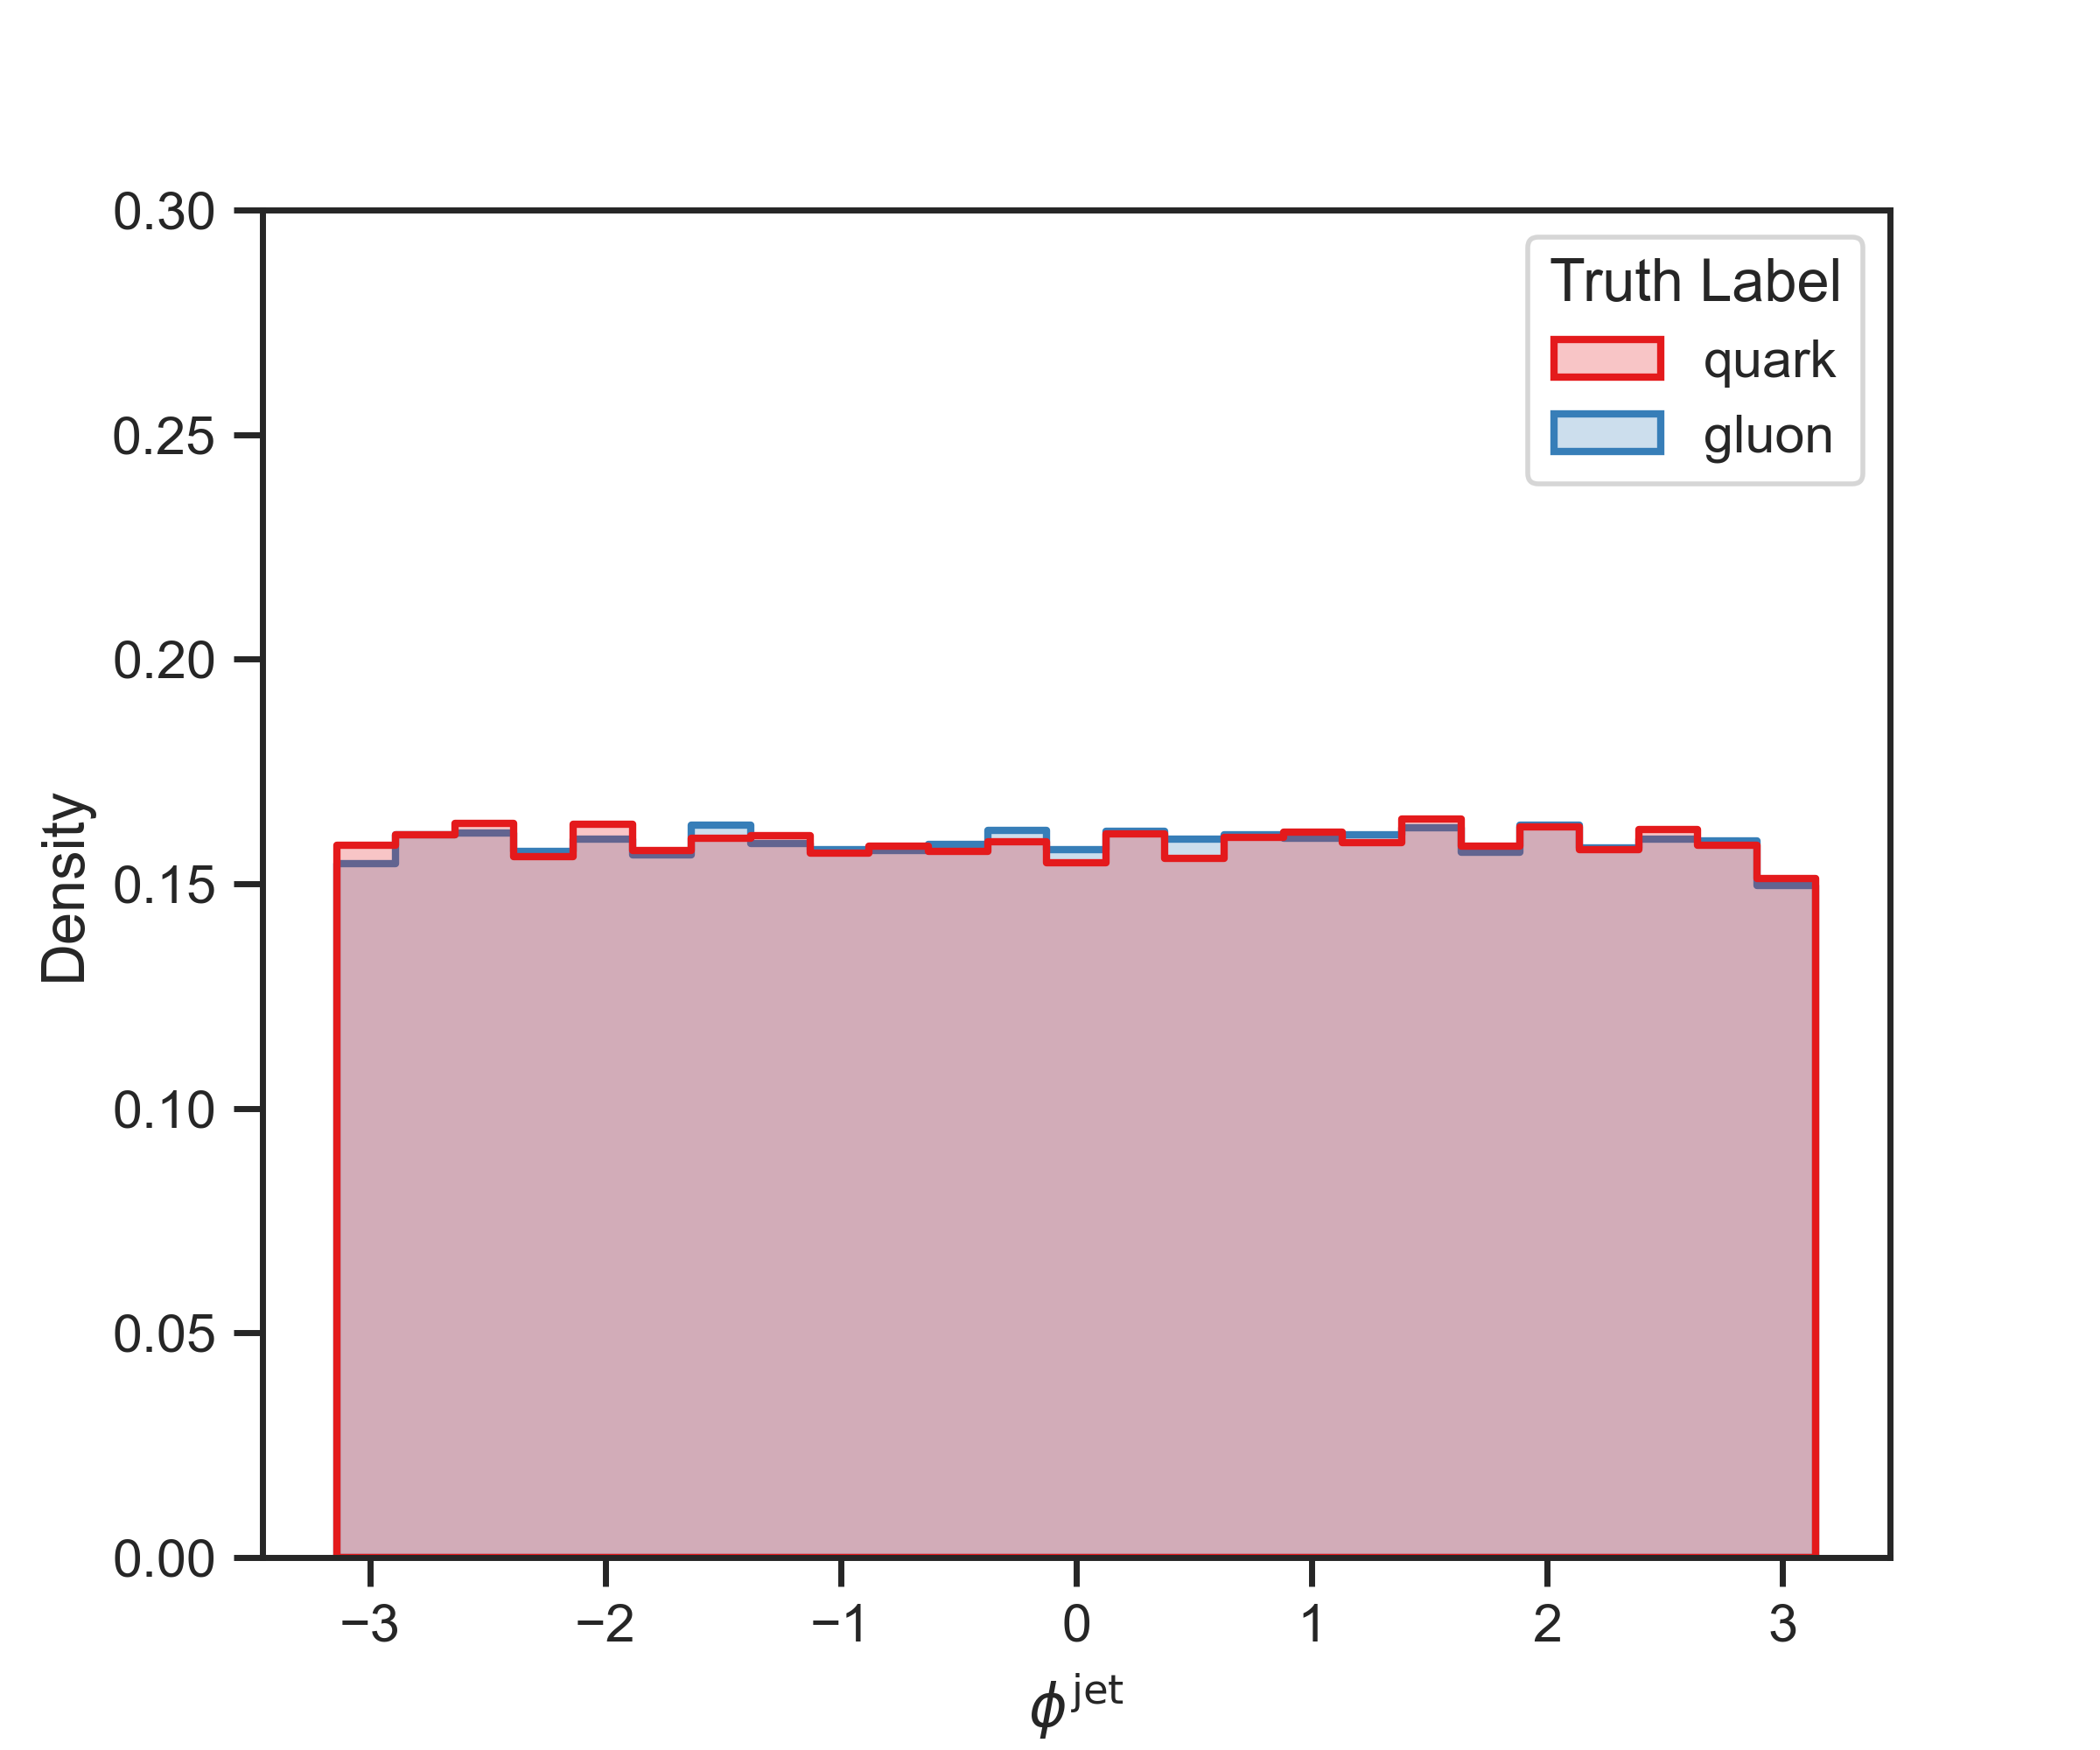
\includegraphics[width=1\textwidth]{src/plots/distributions/highlevel/jets_phi.png}
		\caption{\texttt{jets\_phi}}
		\label{fig:highlevel_28}
	\end{subfigure}
	\begin{subfigure}[t]{0.48\textwidth}
		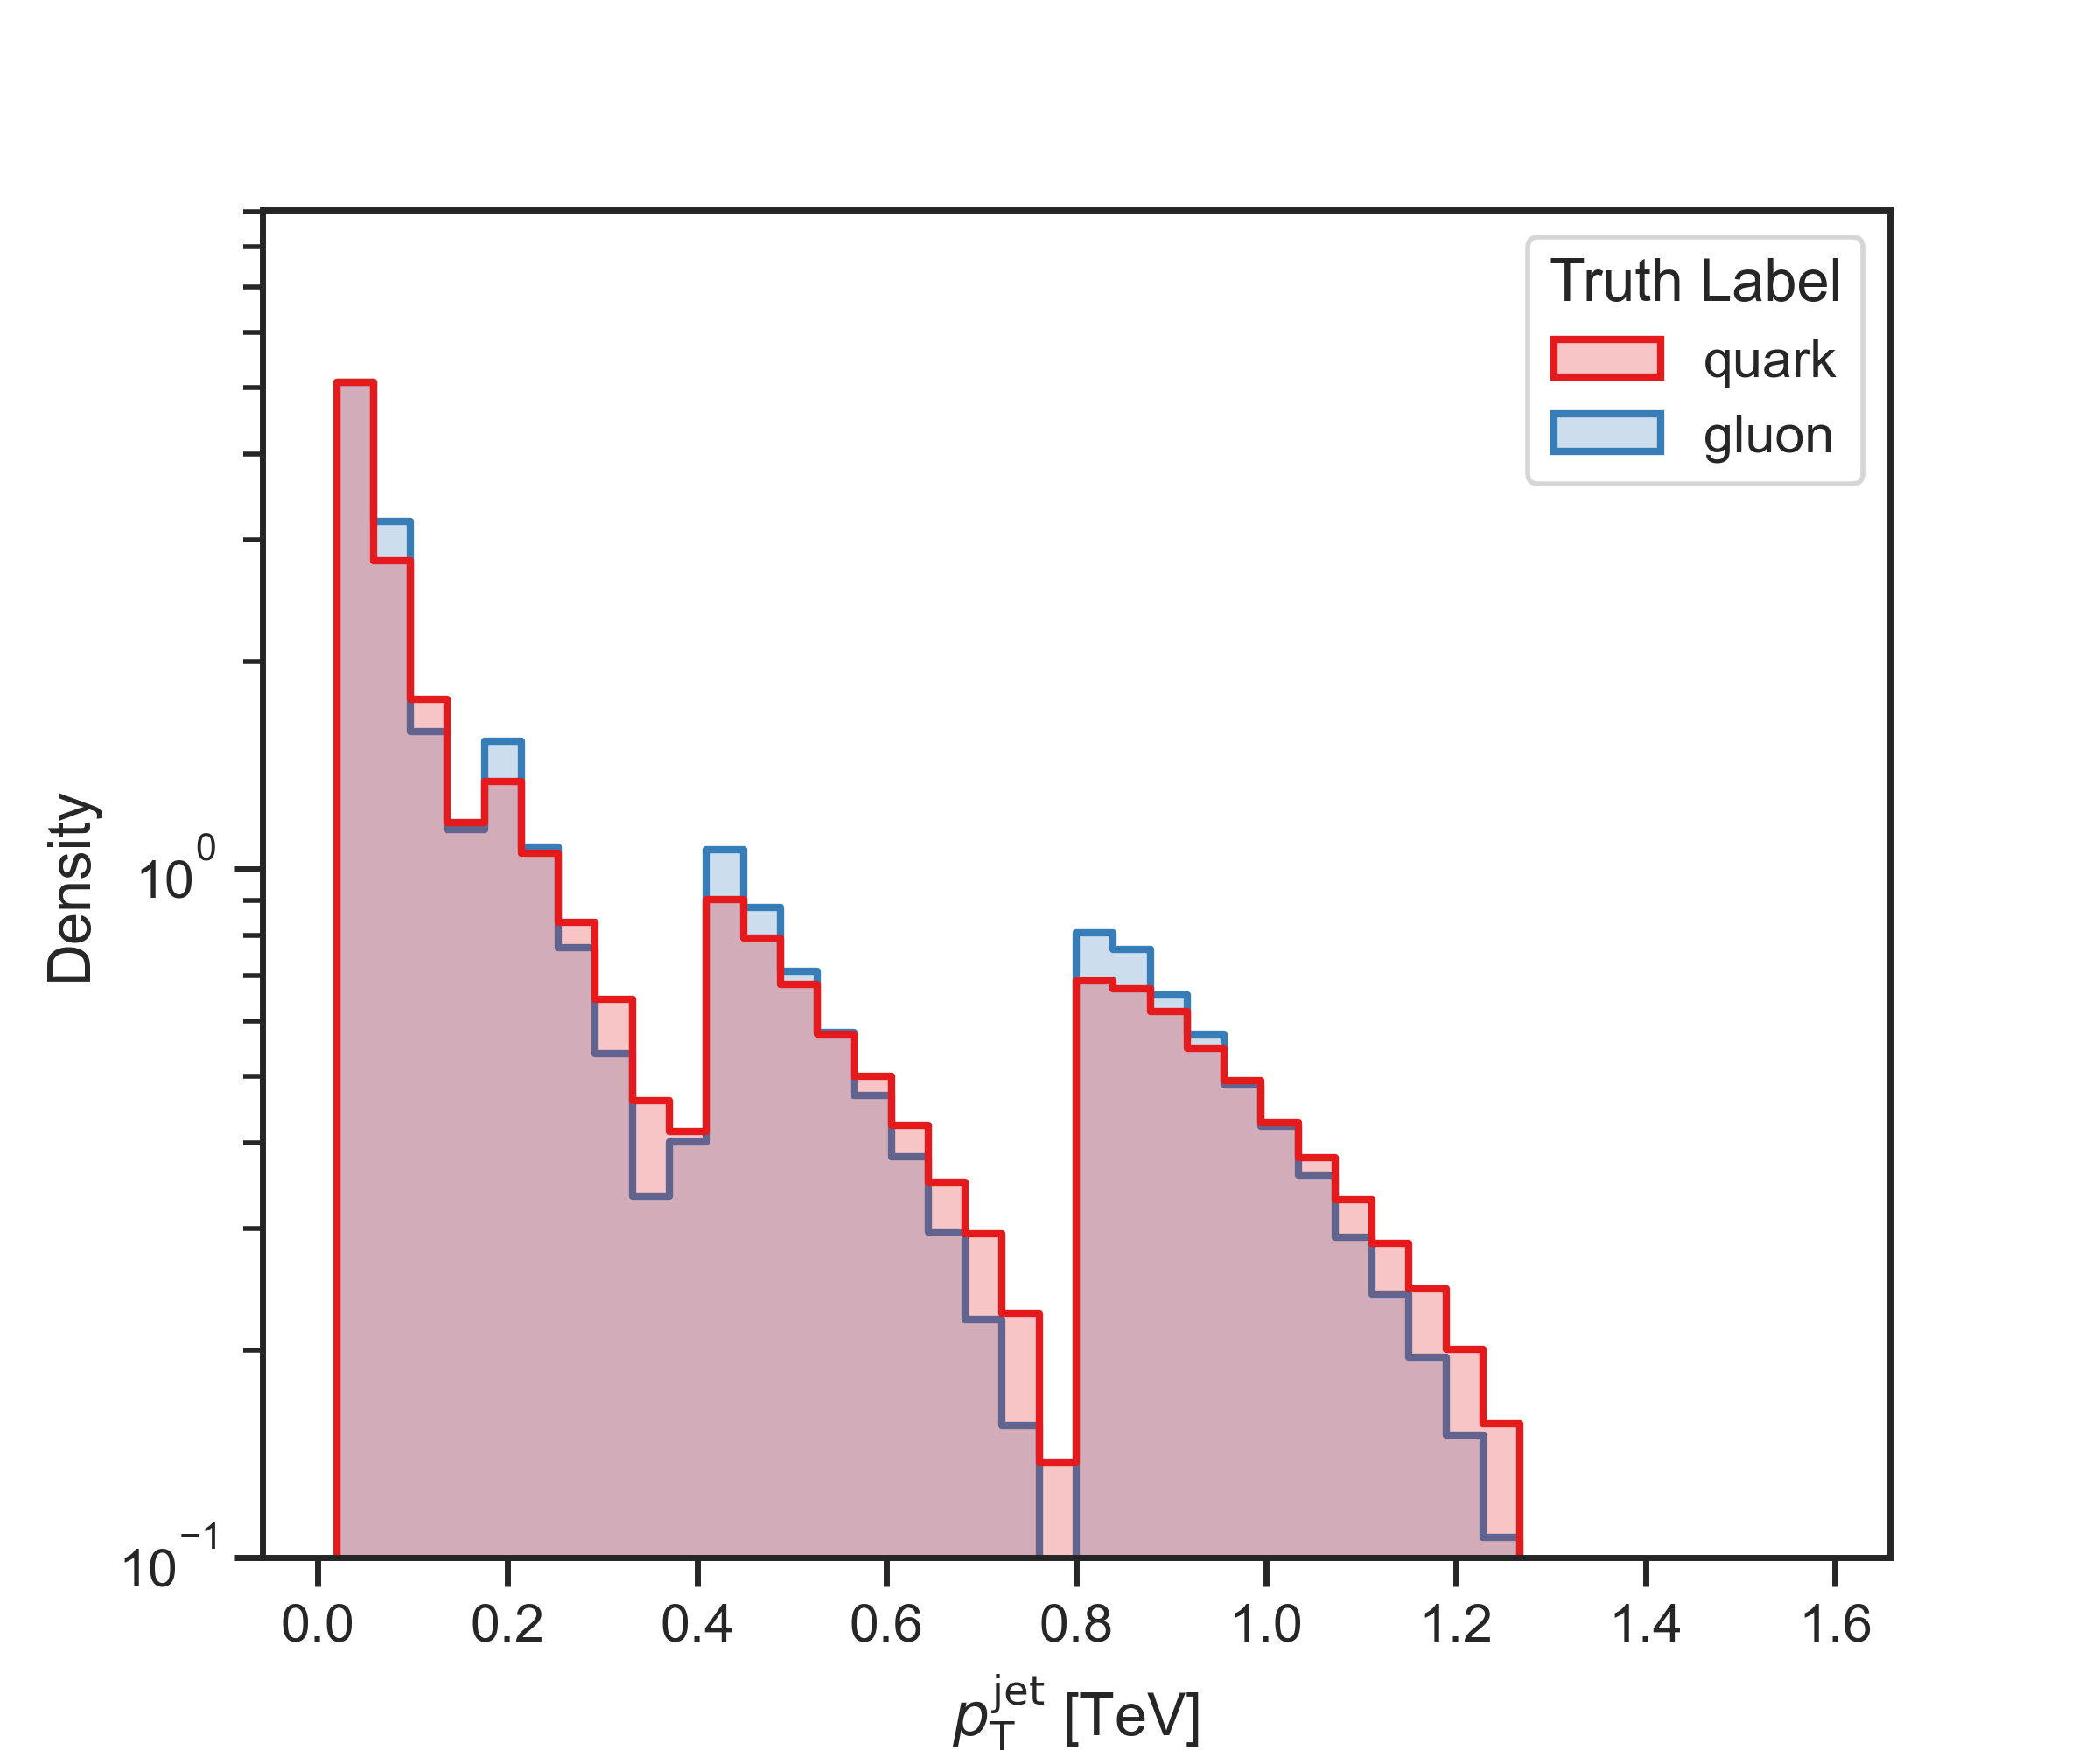
\includegraphics[width=1\textwidth]{src/plots/distributions/highlevel/jets_pt.png}
		\caption{\texttt{jets\_pt}}
		\label{fig:highlevel_29}
	\end{subfigure}
\caption{High-level Jet Variables, part 5}
\label{fig:highlevel_24-29}
\end{figure}




\chapter{Additional Evaluation Plots}
\label{ch:eval}

\section{Confusion Matrix}
\label{sec:app_confusion}

\begin{figure}[!htb]
	\centering
	\begin{subfigure}[t]{0.38\textwidth}
		\includegraphics[width=1\textwidth]{src/plots/results/cm/depart.png}
		\caption{DeParT}
		\label{fig:app_cm_depart}
	\end{subfigure}
	\begin{subfigure}[t]{0.38\textwidth}
		\includegraphics[width=1\textwidth]{src/plots/results/cm/bdt.png}
		\caption{BDT}
		\label{fig:app_cm_bdt}
	\end{subfigure}
	\begin{subfigure}[t]{0.38\textwidth}
		\includegraphics[width=1\textwidth]{src/plots/results/cm/interacting_part.png}
		\caption{Interacting ParT}
		\label{fig:app_cm_interacting_part}
	\end{subfigure}
	\begin{subfigure}[t]{0.38\textwidth}
		\includegraphics[width=1\textwidth]{src/plots/results/cm/highway.png}
		\caption{Highway}
		\label{fig:app_cm_highway}
	\end{subfigure}
\caption{Confusion Matricies}
\label{fig:app_cm_-1-3}
\end{figure}

\begin{figure}[!htb]
	\centering
	\begin{subfigure}[t]{0.38\textwidth}
		\includegraphics[width=1\textwidth]{src/plots/results/cm/fc.png}
		\caption{Fully Connected}
		\label{fig:app_cm_fc}
	\end{subfigure}
	\begin{subfigure}[t]{0.38\textwidth}
		\includegraphics[width=1\textwidth]{src/plots/results/cm/transformer.png}
		\caption{Transformer}
		\label{fig:app_cm_transformer}
	\end{subfigure}
	\begin{subfigure}[t]{0.38\textwidth}
		\includegraphics[width=1\textwidth]{src/plots/results/cm/pfn.png}
		\caption{PFN}
		\label{fig:app_cm_pfn}
	\end{subfigure}
	\begin{subfigure}[t]{0.38\textwidth}
		\includegraphics[width=1\textwidth]{src/plots/results/cm/interacting_depart.png}
		\caption{Interacting DeParT}
		\label{fig:app_cm_interacting_depart}
	\end{subfigure}
	\begin{subfigure}[t]{0.38\textwidth}
		\includegraphics[width=1\textwidth]{src/plots/results/cm/part.png}
		\caption{ParT}
		\label{fig:app_cm_part}
	\end{subfigure}
	\begin{subfigure}[t]{0.38\textwidth}
		\includegraphics[width=1\textwidth]{src/plots/results/cm/efn.png}
		\caption{EFN}
		\label{fig:app_cm_efn}
	\end{subfigure}
\caption{Confusion Matricies}
\label{fig:app_cm_5-9}
\end{figure}



\FloatBarrier
\newpage

\section{Score Histograms}
\label{sec:app_scorehist}

\begin{figure}[!htb]
	\centering
	\begin{subfigure}[t]{0.49\textwidth}
		\includegraphics[width=1\textwidth]{src/plots/results/score/depart.png}
		\caption{DeParT}
		\label{fig:app_score_depart}
	\end{subfigure}
	\begin{subfigure}[t]{0.49\textwidth}
		\includegraphics[width=1\textwidth]{src/plots/results/score/bdt.png}
		\caption{BDT}
		\label{fig:app_score_bdt}
	\end{subfigure}
	\begin{subfigure}[t]{0.49\textwidth}
		\includegraphics[width=1\textwidth]{src/plots/results/score/interacting_part.png}
		\caption{Interacting ParT}
		\label{fig:app_score_interacting_part}
	\end{subfigure}
	\begin{subfigure}[t]{0.49\textwidth}
		\includegraphics[width=1\textwidth]{src/plots/results/score/highway.png}
		\caption{Highway}
		\label{fig:app_score_highway}
	\end{subfigure}
\caption{Confusion Matricies}
\label{fig:app_score_-1-3}
\end{figure}

\begin{figure}[!htb]
	\centering
	\begin{subfigure}[t]{0.49\textwidth}
		\includegraphics[width=1\textwidth]{src/plots/results/score/fc.png}
		\caption{Fully Connected}
		\label{fig:app_score_fc}
	\end{subfigure}
	\begin{subfigure}[t]{0.49\textwidth}
		\includegraphics[width=1\textwidth]{src/plots/results/score/transformer.png}
		\caption{Transformer}
		\label{fig:app_score_transformer}
	\end{subfigure}
	\begin{subfigure}[t]{0.49\textwidth}
		\includegraphics[width=1\textwidth]{src/plots/results/score/pfn.png}
		\caption{PFN}
		\label{fig:app_score_pfn}
	\end{subfigure}
	\begin{subfigure}[t]{0.49\textwidth}
		\includegraphics[width=1\textwidth]{src/plots/results/score/interacting_depart.png}
		\caption{Interacting DeParT}
		\label{fig:app_score_interacting_depart}
	\end{subfigure}
	\begin{subfigure}[t]{0.49\textwidth}
		\includegraphics[width=1\textwidth]{src/plots/results/score/part.png}
		\caption{ParT}
		\label{fig:app_score_part}
	\end{subfigure}
	\begin{subfigure}[t]{0.49\textwidth}
		\includegraphics[width=1\textwidth]{src/plots/results/score/efn.png}
		\caption{EFN}
		\label{fig:app_score_efn}
	\end{subfigure}
\caption{Confusion Matricies}
\label{fig:app_score_5-9}
\end{figure}



\FloatBarrier

\section{Transverse Momentum Dependence}
\label{sec:app_pt_dep}


\begin{figure}[htb]
    \centering
    \includegraphics[width=0.95\linewidth]{src/plots/results/pT_dep/auc.jpg}
    \caption{AUC as a function of transverse momentum.}
    \label{fig:auc_pt}
\end{figure}

\begin{figure}[htb]
    \centering
    \includegraphics[width=0.95\linewidth]{src/plots/results/pT_dep/gluon_efficiency.jpg}
    \caption{Gluon efficiency as a function of transverse momentum.}
    \label{fig:gluon_eff_pt}
\end{figure}

\begin{figure}[htb]
    \centering
    \includegraphics[width=0.95\linewidth]{src/plots/results/pT_dep/quark_efficiency.jpg}
    \caption{Quark efficiency as a function of transverse momentum.}
    \label{fig:quark_eff_pt}
\end{figure}

\begin{figure}[htb]
    \centering
    \includegraphics[width=0.95\linewidth]{src/plots/results/pT_dep/gluon_rejection.jpg}
    \caption{Gluon rejection as a function of transverse momentum.}
    \label{fig:gluon_rej_pt}
\end{figure}

\begin{figure}[htb]
    \centering
    \includegraphics[width=0.95\linewidth]{src/plots/results/pT_dep/quark_rejection.jpg}
    \caption{Quark rejection as a function of transverse momentum.}
    \label{fig:quark_rej_pt}
\end{figure}

\begin{figure}[htb]
    \centering
    \includegraphics[width=0.95\linewidth]{src/plots/results/pT_dep/quark_rej_at_gluon_eff_0.9.jpg}
    \caption{Quark rejection at gluon efficiency of 0.9 as a function of transverse momentum.}
    \label{fig:quark_rej_at_gluon_eff_0.9_pt}
\end{figure}

\begin{figure}[htb]
    \centering
    \includegraphics[width=0.95\linewidth]{src/plots/results/pT_dep/gluon_rej_at_quark_eff_0.9.jpg}
    \caption{Gluon rejection at quark efficiency of 0.9 as a function of transverse momentum.}
    \label{fig:gluon_rej_at_quark_eff_0.9_pt}
\end{figure}

\begin{figure}[htb]
    \centering
    \includegraphics[width=0.95\linewidth]{src/plots/results/pT_dep/loss.jpg}
    \caption{Loss as a function of transverse momentum.}
    \label{fig:loss_pt}
\end{figure}

\FloatBarrier

\section{Pseudo-rapidity Dependence}
\label{sec:app_eta_dep}

\begin{figure}[htb]
    \centering
    \includegraphics[width=0.95\linewidth]{src/plots/results/eta_dep/auc.jpg}
    \caption{AUC as a function of pseudo-rapidity.}
    \label{fig:auc_eta}
\end{figure}

\begin{figure}[htb]
    \centering
    \includegraphics[width=0.95\linewidth]{src/plots/results/eta_dep/gluon_efficiency.jpg}
    \caption{Gluon efficiency as a function of pseudo-rapidity.}
    \label{fig:gluon_eff_eta}
\end{figure}

\begin{figure}[htb]
    \centering
    \includegraphics[width=0.95\linewidth]{src/plots/results/eta_dep/quark_efficiency.jpg}
    \caption{Quark efficiency as a function of pseudo-rapidity.}
    \label{fig:quark_eff_eta}
\end{figure}

\begin{figure}[htb]
    \centering
    \includegraphics[width=0.95\linewidth]{src/plots/results/eta_dep/gluon_rejection.jpg}
    \caption{Gluon rejection as a function of pseudo-rapidity.}
    \label{fig:gluon_rej_eta}
\end{figure}

\begin{figure}[htb]
    \centering
    \includegraphics[width=0.95\linewidth]{src/plots/results/eta_dep/quark_rejection.jpg}
    \caption{Quark rejection as a function of pseudo-rapidity.}
    \label{fig:quark_rej_eta}
\end{figure}

\begin{figure}[htb]
    \centering
    \includegraphics[width=0.95\linewidth]{src/plots/results/eta_dep/quark_rej_at_gluon_eff_0.9.jpg}
    \caption{Quark rejection at gluon efficiency of 0.9 as a function of pseudo-rapidity.}
    \label{fig:quark_rej_at_gluon_eff_0.9_eta}
\end{figure}

\begin{figure}[htb]
    \centering
    \includegraphics[width=0.95\linewidth]{src/plots/results/eta_dep/gluon_rej_at_quark_eff_0.9.jpg}
    \caption{Gluon rejection at quark efficiency of 0.9 as a function of pseudo-rapidity.}
    \label{fig:gluon_rej_at_quark_eff_0.9_eta}
\end{figure}

\begin{figure}[htb]
    \centering
    \includegraphics[width=0.95\linewidth]{src/plots/results/eta_dep/loss.jpg}
    \caption{Loss as a function of pseudo-rapidity.}
    \label{fig:loss_eta}
\end{figure}

\FloatBarrier

\section{Pileup Dependence}
\label{sec:app_pileup_dep}

\begin{figure}[htb]
    \centering
    \includegraphics[width=0.95\linewidth]{src/plots/results/mu_dep/auc.jpg}
    \caption{AUC as a function of pileup.}
    \label{fig:auc_pileup}
\end{figure}

\begin{figure}[htb]
    \centering
    \includegraphics[width=0.95\linewidth]{src/plots/results/mu_dep/gluon_efficiency.jpg}
    \caption{Gluon efficiency as a function of pileup.}
    \label{fig:gluon_eff_pileup}
\end{figure}

\begin{figure}[htb]
    \centering
    \includegraphics[width=0.95\linewidth]{src/plots/results/mu_dep/quark_efficiency.jpg}
    \caption{Quark efficiency as a function of pileup.}
    \label{fig:quark_eff_pileup}
\end{figure}

\begin{figure}[htb]
    \centering
    \includegraphics[width=0.95\linewidth]{src/plots/results/mu_dep/gluon_rejection.jpg}
    \caption{Gluon rejection as a function of pileup.}
    \label{fig:gluon_rej_pileup}
\end{figure}

\begin{figure}[htb]
    \centering
    \includegraphics[width=0.95\linewidth]{src/plots/results/mu_dep/quark_rejection.jpg}
    \caption{Quark rejection as a function of pileup.}
    \label{fig:quark_rej_pileup}
\end{figure}

\begin{figure}[htb]
    \centering
    \includegraphics[width=0.95\linewidth]{src/plots/results/mu_dep/quark_rej_at_gluon_eff_0.9.jpg}
    \caption{Quark rejection at gluon efficiency of 0.9 as a function of pileup.}
    \label{fig:quark_rej_at_gluon_eff_0.9_pileup}
\end{figure}

\begin{figure}[htb]
    \centering
    \includegraphics[width=0.95\linewidth]{src/plots/results/mu_dep/gluon_rej_at_quark_eff_0.9.jpg}
    \caption{Gluon rejection at quark efficiency of 0.9 as a function of pileup.}
    \label{fig:gluon_rej_at_quark_eff_0.9_pileup}
\end{figure}

\begin{figure}[htb]
    \centering
    \includegraphics[width=0.95\linewidth]{src/plots/results/mu_dep/loss.jpg}
    \caption{Loss as a function of pileup.}
    \label{fig:loss_pileup}
\end{figure}


  

% if your attachments are complicated, describe them in a separate appendix
%\include{attachments}

\openright
\end{document}
